\documentclass[10pt,a4paper]{article}
\usepackage{graphicx}
\usepackage{subfig}
\usepackage{svg}

%%%%%%%%%%%%%%%%%%%%%%%%%%%
% MODIFY:

\newcommand{\authorA}{Jia Long Ji Qiu}
\newcommand{\authorB}{Jiabo Wang}
\newcommand{\authorC}{Yilun Liu}
\newcommand{\groupNumber}{J} % - YOUR GROUP NUMBER
\newcommand{\exerciseNumber}{2} % - THE NUMBER OF THE EXERCISE
\newcommand{\sourceCodeLink}{https://github.com/jialongjq/mlcms}

\newcommand{\workPerAuthor}{
\authorA&Task 1&1/3\%\\
      &Task 2&1/3\%\\
      &Task 3&1/3\%\\
      &Task 4&1/3\%\\
      &Task 5&1/3\%\\
      \hline
\authorB&Task 1&1/3\%\\
      &Task 2&1/3\%\\
      &Task 3&1/3\%\\
      &Task 4&1/3\%\\
      &Task 5&1/3\%\\
      \hline
\authorC&Task 1&1/3\%\\
      &Task 2&1/3\%\\
      &Task 3&1/3\%\\
      &Task 4&1/3\%\\
      &Task 5&1/3\%
}

%%%%%%%%%%%%%%%%%%%%%%%%%%%

%%
% imports for the exercise sheets
%

\usepackage[utf8]{inputenc}
\usepackage{amsmath}
\usepackage{amsfonts}
\usepackage{amssymb}

\usepackage[yyyymmdd]{datetime}
\renewcommand{\dateseparator}{--}

\usepackage[left=2cm,right=2cm,top=3cm,bottom=3cm]{geometry}
\usepackage{listings, xcolor}

\definecolor{codegreen}{rgb}{0,0.6,0}
\definecolor{codegray}{rgb}{0.5,0.5,0.5}
\definecolor{codepurple}{rgb}{0.58,0,0.82}
\definecolor{backcolour}{rgb}{0.95,0.95,0.92}

\lstdefinestyle{mystyle}{
    backgroundcolor=\color{backcolour},   
    commentstyle=\color{codegreen},
    keywordstyle=\color{magenta},
    numberstyle=\tiny\color{codegray},
    stringstyle=\color{codepurple},
    basicstyle=\ttfamily\footnotesize,
    breakatwhitespace=false,         
    breaklines=true,                 
    captionpos=b,                    
    keepspaces=true,               
    showspaces=false,                
    showstringspaces=false,
    showtabs=false,                  
    tabsize=2
}

\lstset{style=mystyle}

\usepackage{hyperref}

\usepackage{amsthm}
\newtheorem{lem}{Lemma}
\newtheorem{thm}{Theorem}
\newtheorem{cor}{Corollary}
\newtheorem{rem}{Remark}
\newtheorem{definition}{Definition}
\newtheorem{ter}{Terminology}

\usepackage{graphicx}

\newcommand{\M}{\mathcal{M}}
\newcommand{\N}{\mathcal{N}}
\newcommand{\K}{\mathcal{K}}
\newcommand{\SPDk}{\mathbb{P}^k}
\newcommand{\vol}{\text{vol}}

\newcommand{\Figref}[1]{Figure~\ref{#1}}
\newcommand{\figref}[1]{figure~\ref{#1}}
\newcommand{\Eqnref}[1]{Equation~(\eqref{#1})}
\newcommand{\eqnref}[1]{equation~(\eqref{#1})}

\usepackage{float}
\usepackage{tabularx}

\usepackage{fancyhdr}
\pagestyle{fancy}

\usepackage{totcount}
\newtotcounter{taskCounter}
\newtotcounter{pointCounter}
\newenvironment{task}[1]{\noindent\stepcounter{taskCounter}\textbf{Report on task #1}\smallbreak\hrule\smallbreak}{\smallbreak\hrule\bigbreak}

\usepackage{array}

\usepackage{caption}
\usepackage{subcaption}

\title{Report for exercise \exerciseNumber~from group~\groupNumber}

\makeatletter
\let\thetitle\@title
\let\theauthor\@author
\let\thedate\@date
\makeatother

\providecommand{\versiondate}{\today}

\lhead{Exercise sheet \exerciseNumber}
\chead{Master Praktikum: Modelling and Simulation of Crowds WS2022/23}
\rhead{TUM}
\lfoot{Report of Group \groupNumber}
\cfoot{\thepage}
\rfoot{Last compiled: \versiondate}
\renewcommand{\headrulewidth}{0.4pt}
\renewcommand{\footrulewidth}{0.4pt}

\newcommand{\frontpage}{
\begin{center}
\textbf{\thetitle}\\~\\
\end{center}
\begin{table}[H]
\begin{tabular}{ll}
Tasks addressed:&\total{taskCounter}\\
Authors:&\authorA\\
&\authorB\\
&\authorC\\
Last compiled:&\versiondate\\
Source code:&\sourceCodeLink
\end{tabular}
\end{table}
\vfill
The work on tasks was divided in the following way:
\begin{table}[H]
\begin{tabularx}{\textwidth}{X|p{2cm}|p{2cm}}
\workPerAuthor
\end{tabularx}
\end{table}
\newpage
}

\begin{document}

\frontpage

\begin{task}{1, Setting up the Vadere environment}

\noindent{\textbf{General overview of Vadere}}

Making first a general comparison between Vadere and the cellular automaton of the first exercise, there are various aspects that should be highlighted.

First of all, the interface of Vadere offers a wide variety of options that are very intuitive and makes the set up of any scenario much easier. The visualisation is similar to the one of the cellular automaton, since it consists of cells as well, with the plus of the elements being able to occupy larger sizes.

Moreover, when it comes to the visualisation of a simulation, it is really convenient that the results are saved as an output, so the user can check them again at any time. The same goes for the progress bar, which allows the visualisation frame by frame of the results.

One last feature to highlight would be the file system. Vadere allows both loading and saving files for different purposes, which can be for example loading or saving a whole project, add predefined scenarios, changing parameters of a simulation such as the model, the psychology, the topology...

\bigskip

\noindent{\textbf{RiMEA scenario 1 (straight line)}}

It should be recalled that the RiMEA scenario 1 defined a 2 m wide and 40
m long corridor, with a pedestrian in one side and its target in the other one, with the purpose of proving that a pedestrian with a defined walking speed will cover the distance in the corresponding time period.

This scenario has been set up with the Vadere environment as shown in Figure \ref{scenario_1a}. For proper visualisation purposes, both width and height have been set to 40 m, and two obstacles of dimensions 40x19 have been placed to leave a 2 m wide space in the middle. The pedestrian was defined with a free flow speed of 1.33 m/s, so the travel time should lie in the range of 26 to 34 seconds. The pre-movement time is ignored since the pedestrian has its target assigned manually before running the simulation. The standard template Optimal Steps Model has been set for this execution, as well as for the rest of the scenarios of this task (RiMEA scenario 6 and chicken test).

As expected, by looking at the results of the simulation (Figure \ref{scenario_1c}), the travel time was around 30 seconds. Compared with the results of the cellular automaton created in exercise 1, the behaviour of the pedestrian is roughly the same (as it should be), since the only thing the pedestrian has to do is to walk in a straight line.
\begin{figure} [H]
 \centering
  \subfloat[At the beginning of the simulation]{
   \label{scenario_1a}
    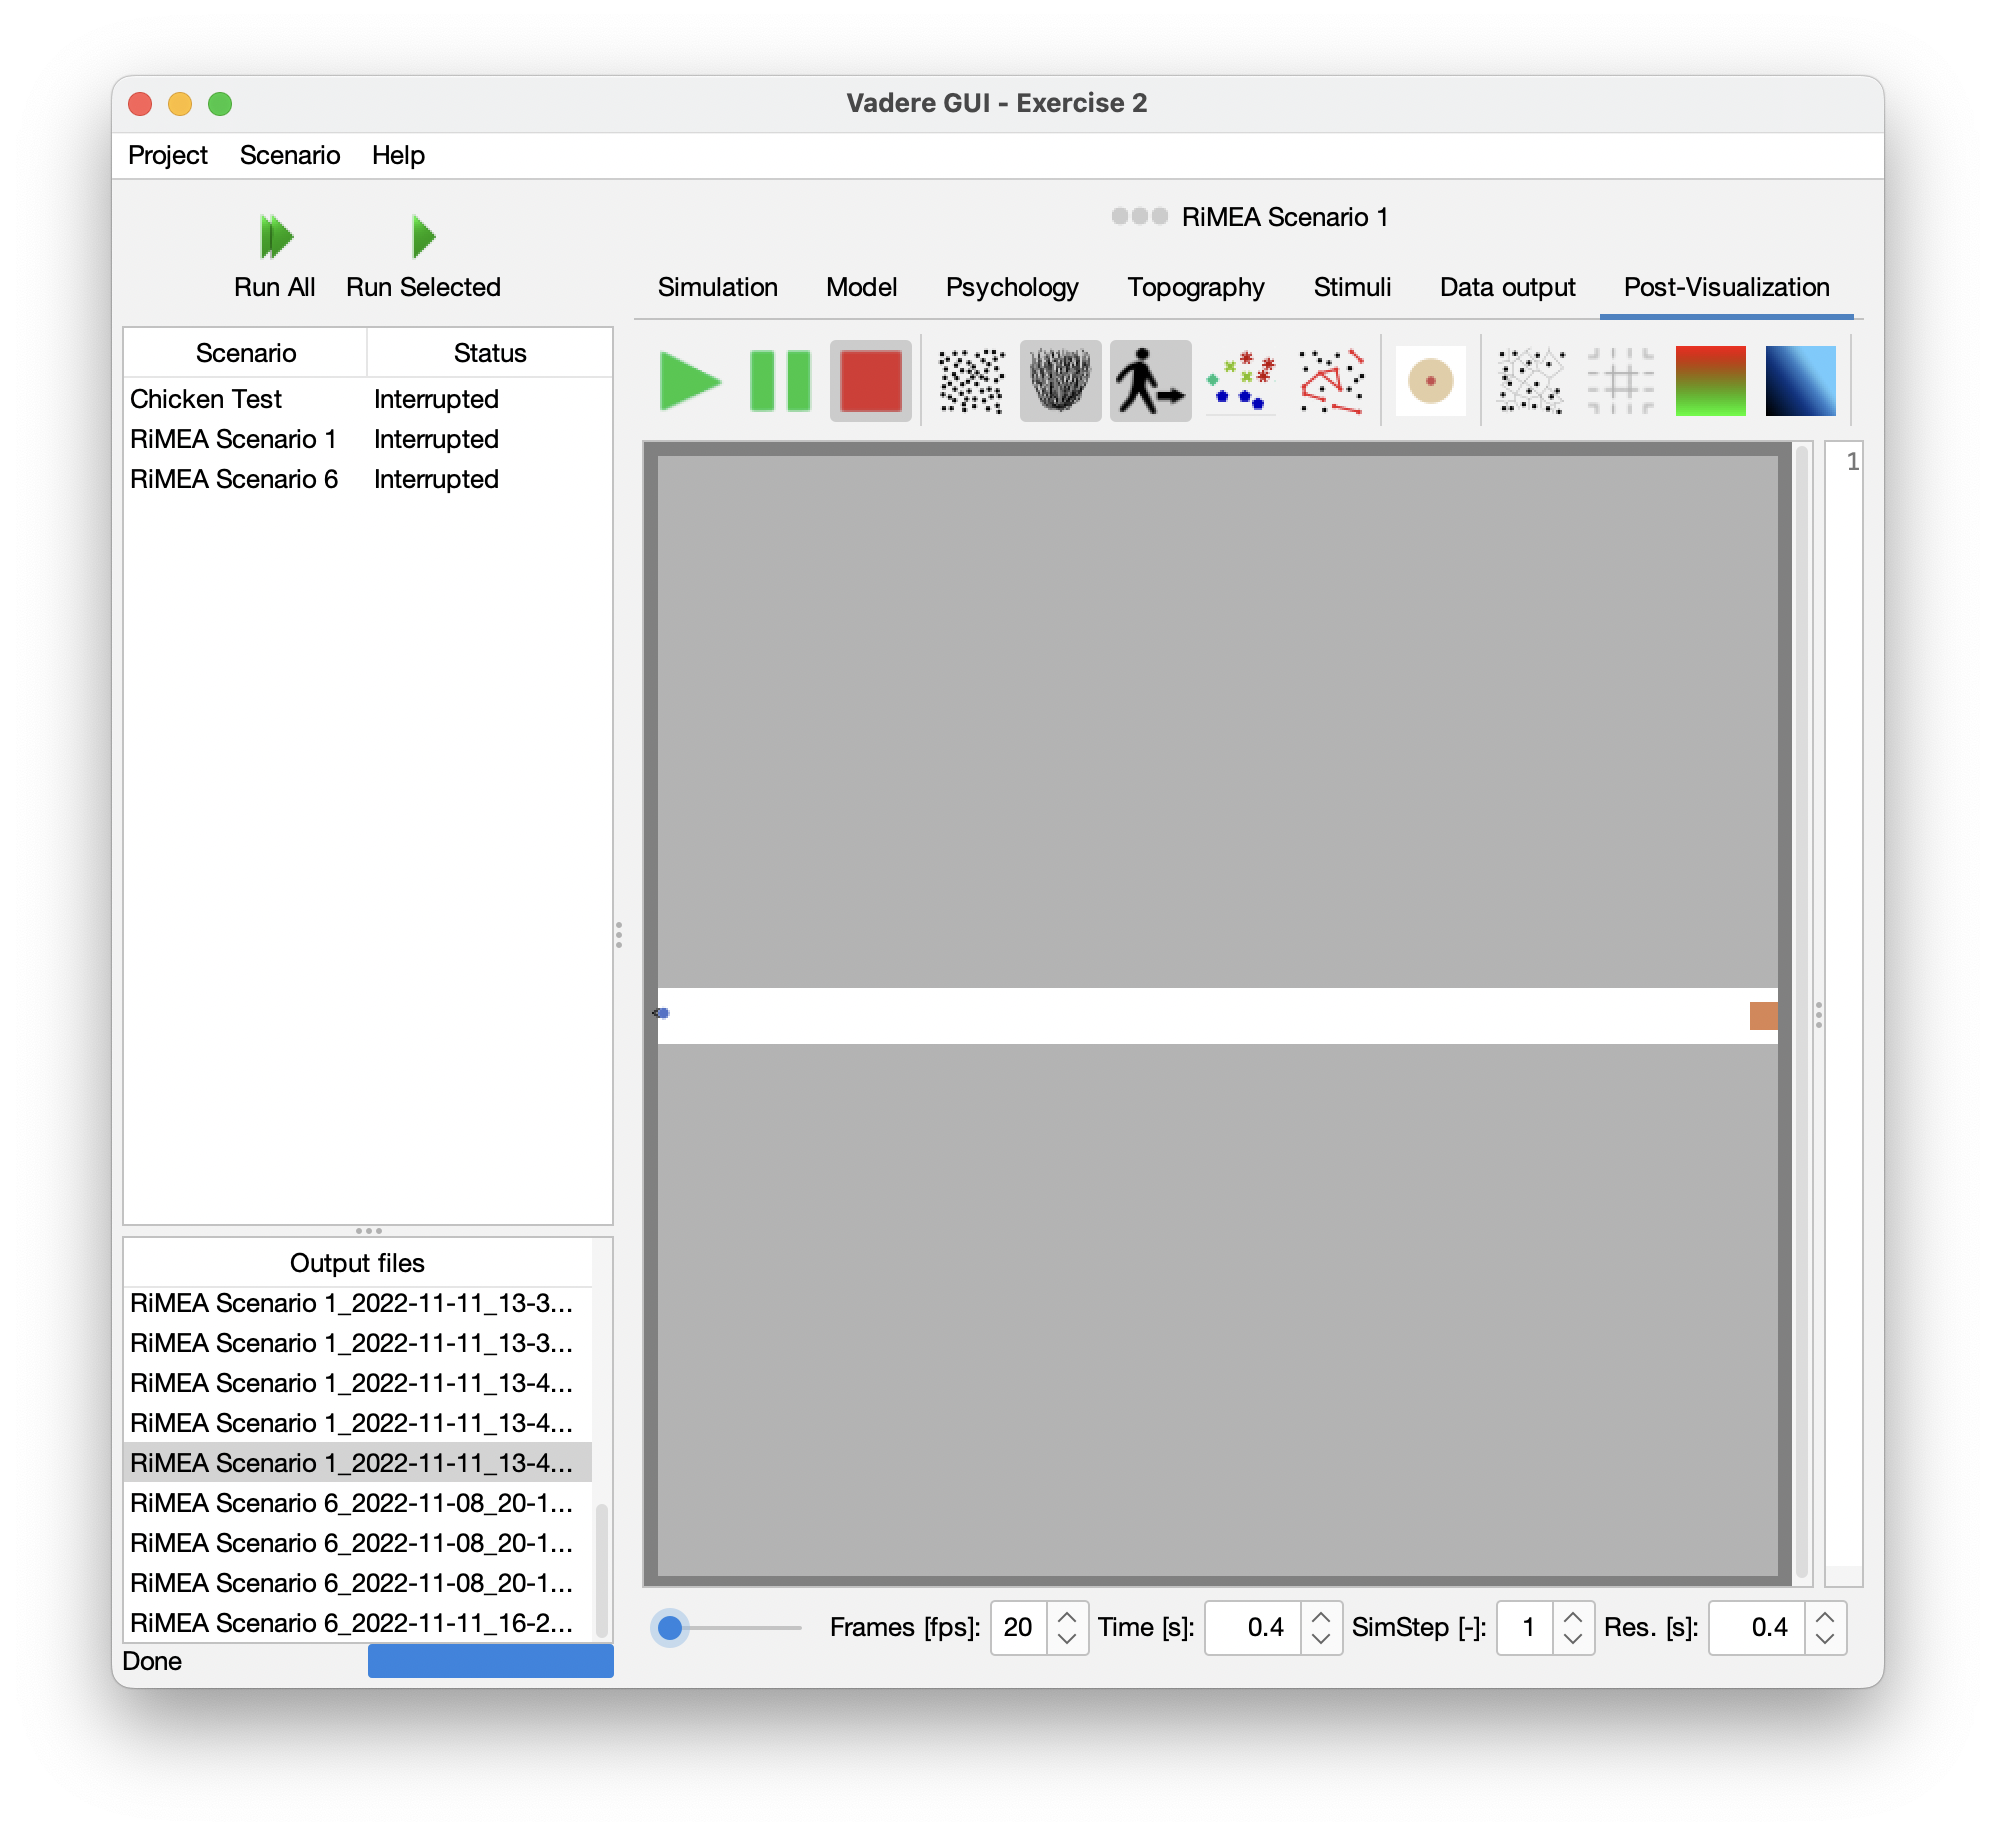
\includegraphics[width=0.33\textwidth]{images/scenario_1a.png}}
  \subfloat[In the middle of the simulation]{
   \label{scenario_1b}
    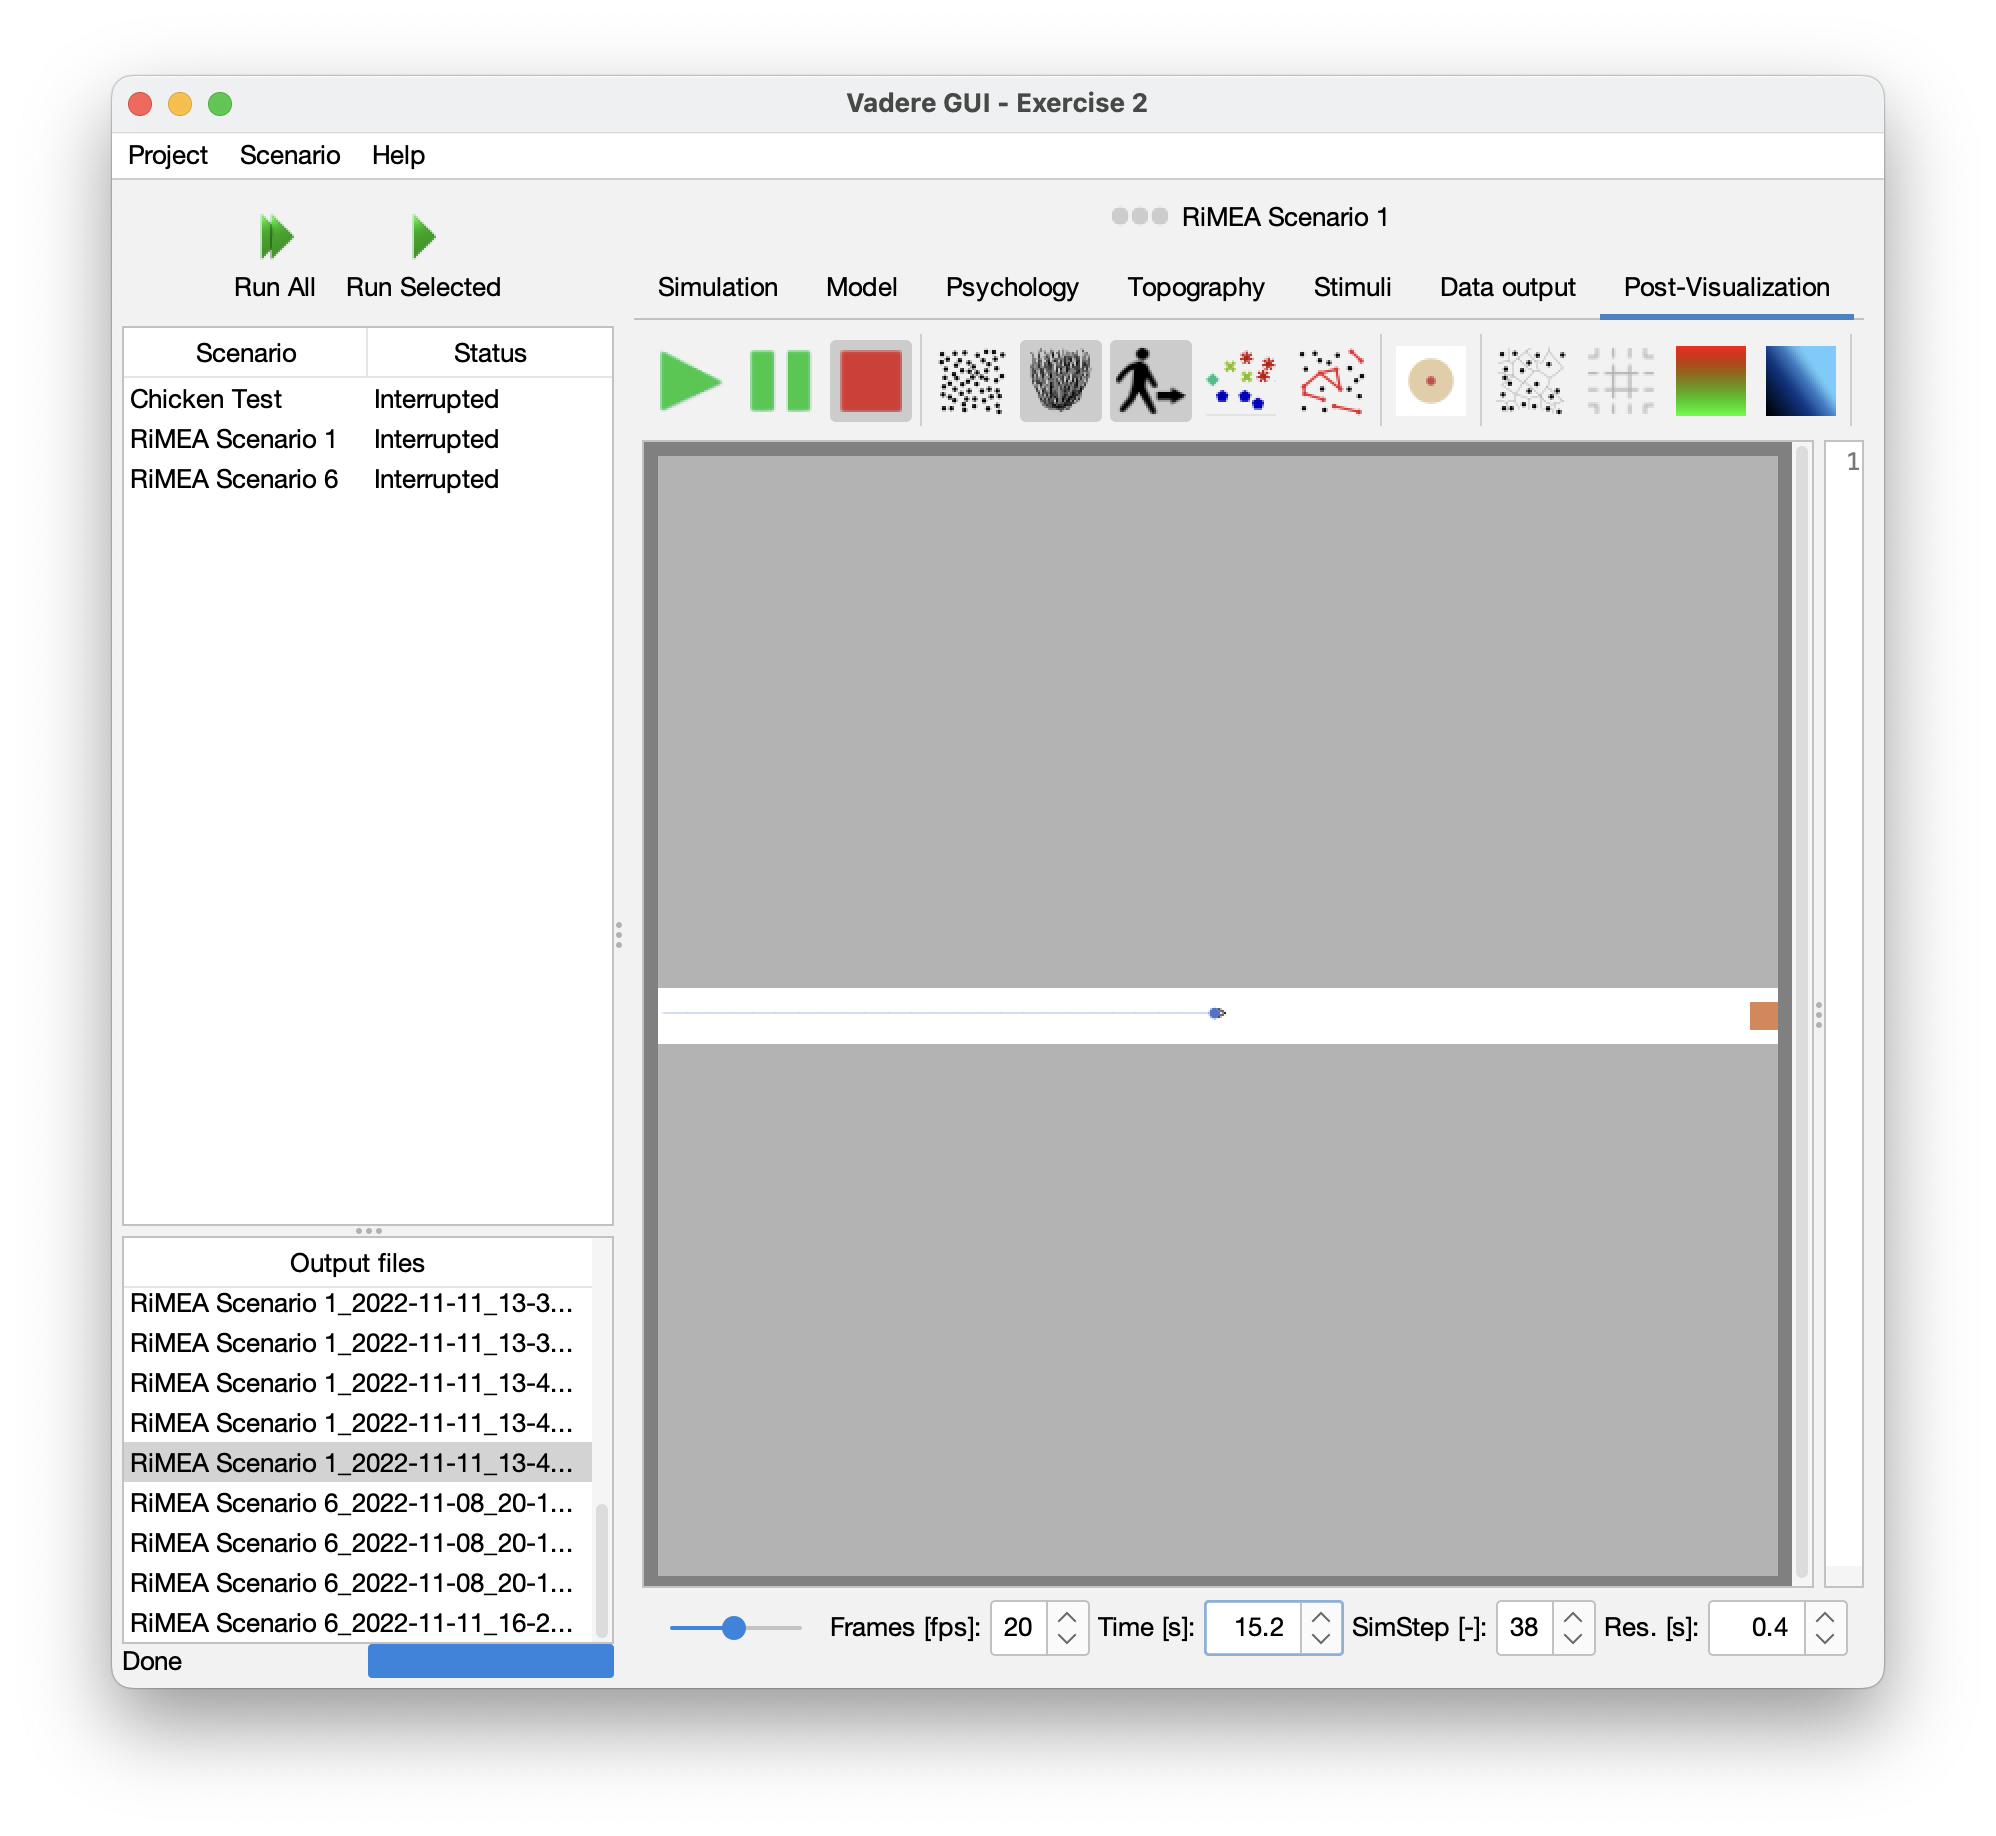
\includegraphics[width=0.33\textwidth]{images/scenario_1b.png}}
  \subfloat[At the end of the simulation]{
   \label{scenario_1c}
    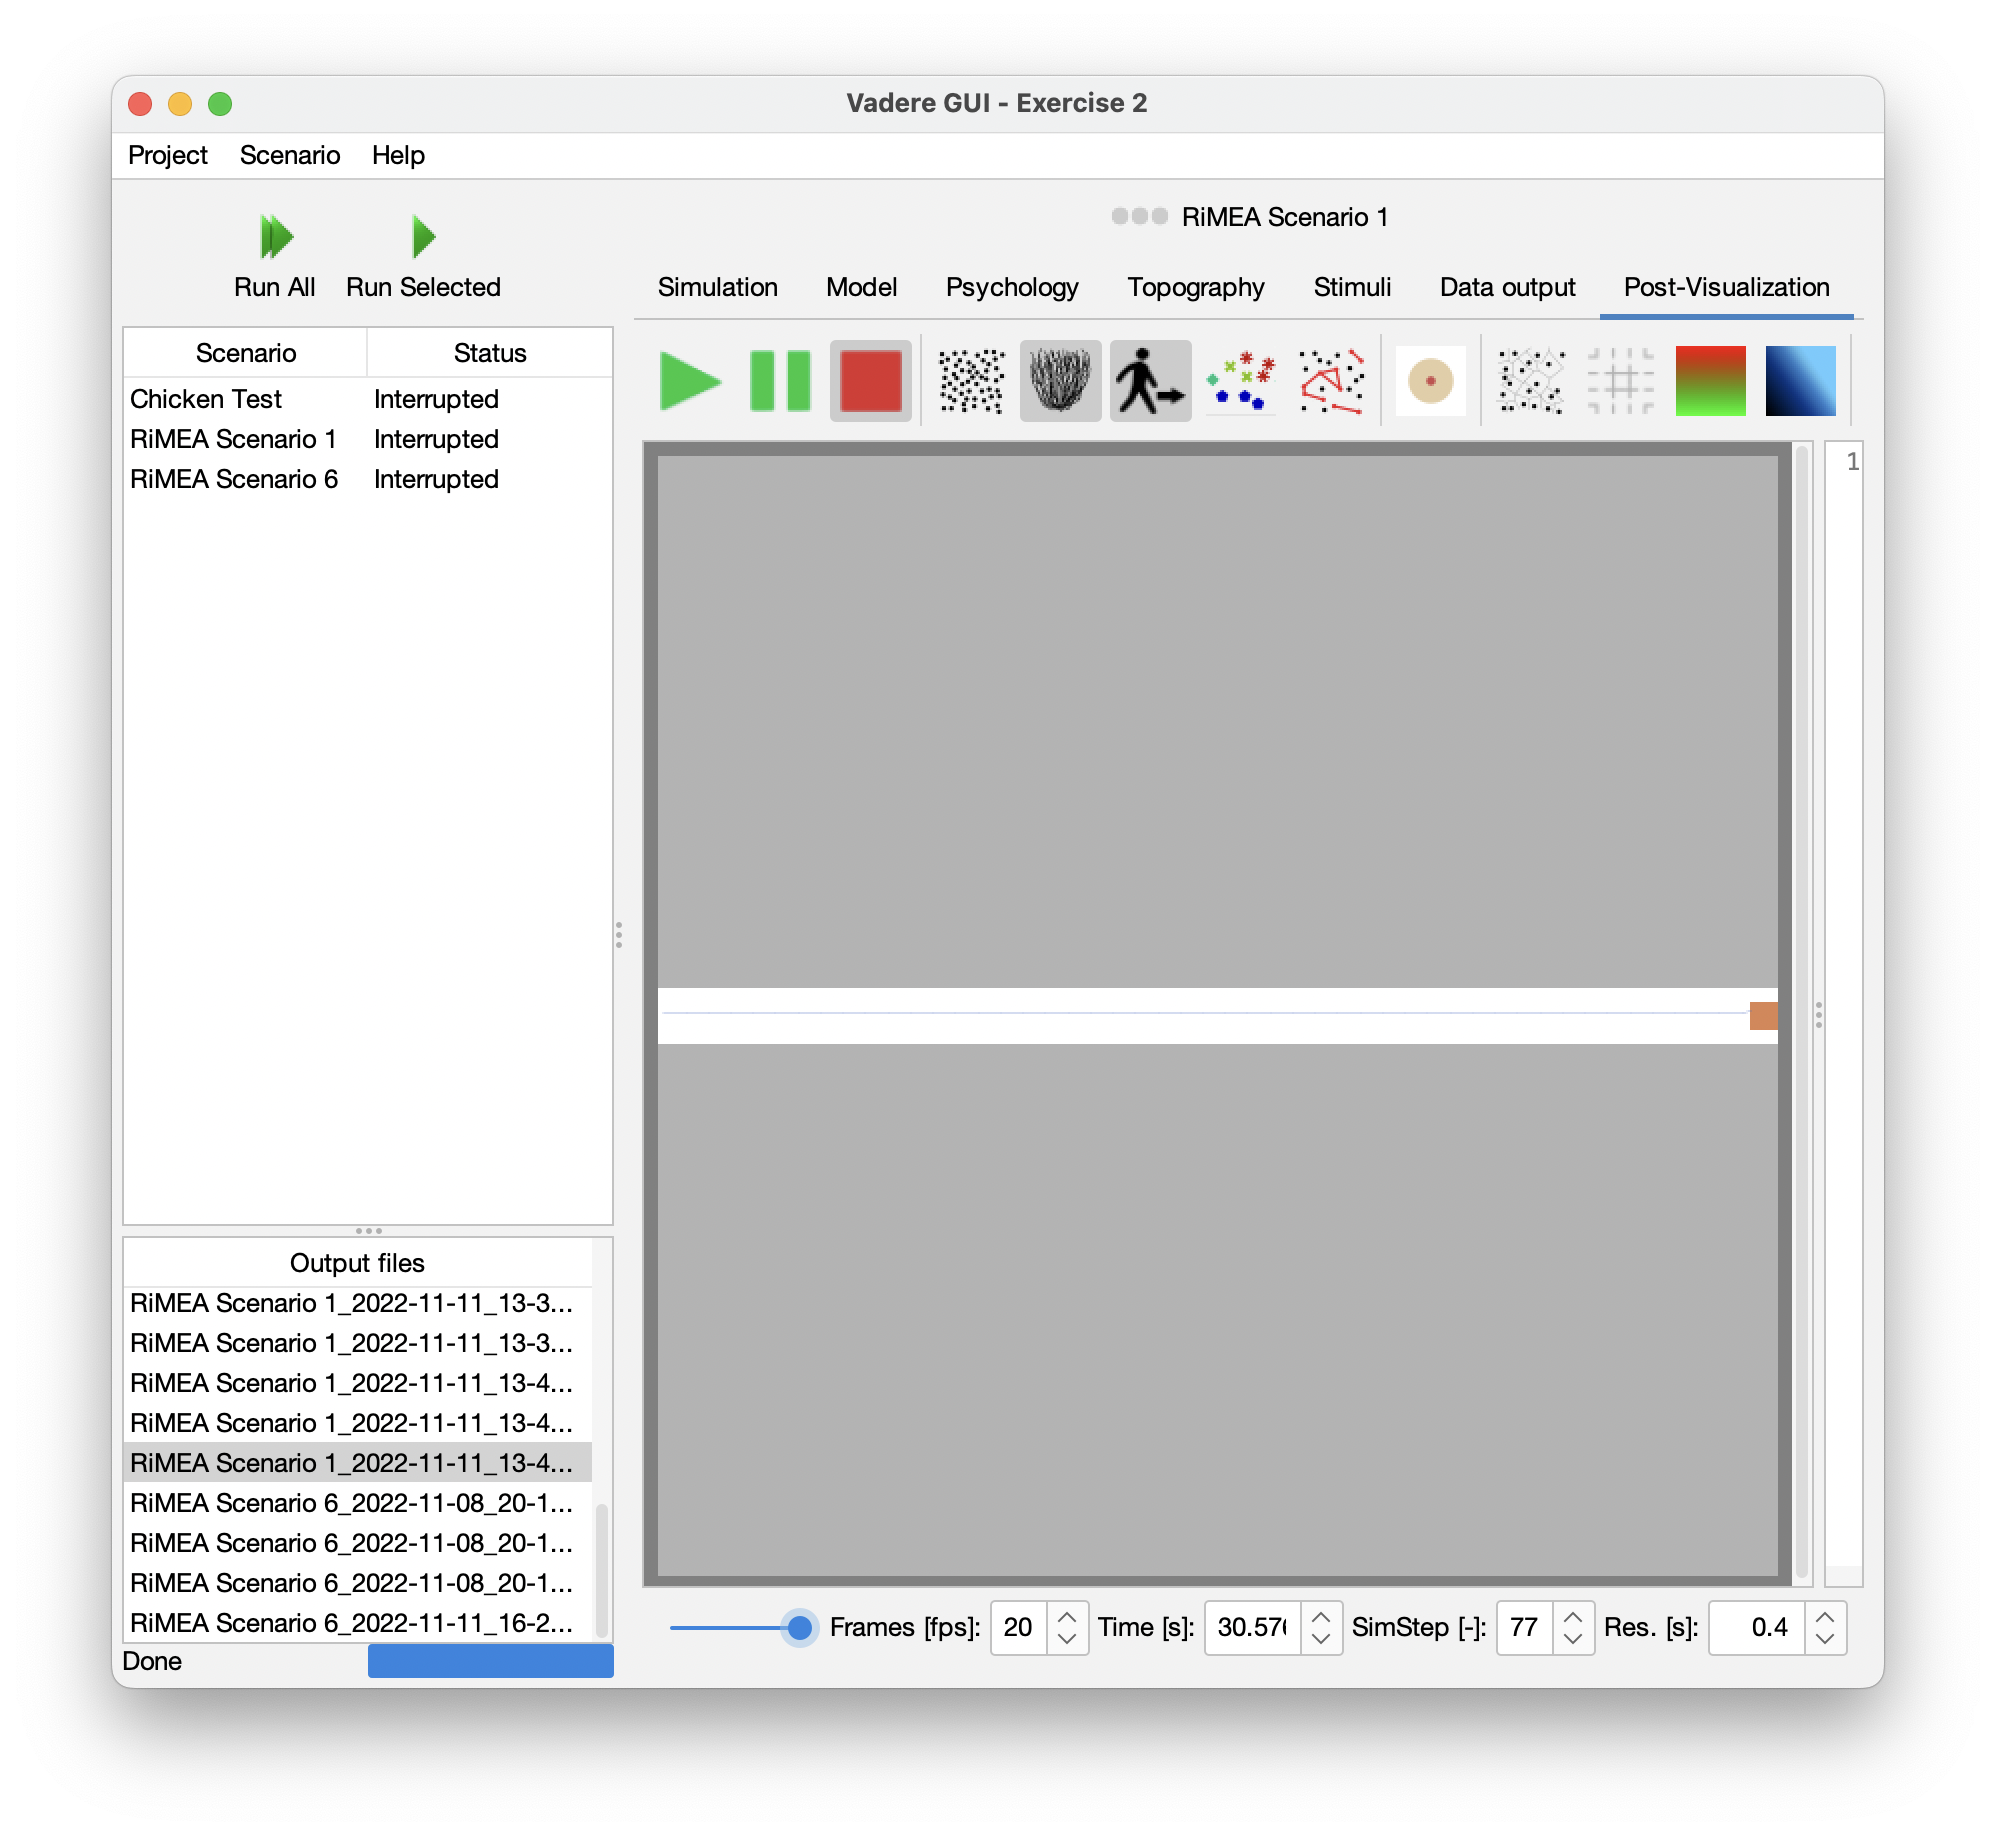
\includegraphics[width=0.33\textwidth]{images/scenario_1c.png}}
 \caption{Different stages of the simulation of the scenario 1}
 \label{scenario1_sim}
\end{figure}

\clearpage

\noindent{\textbf{RiMEA scenario 6 (corner)}}

The RiMEA scenario 6 describes a group of 20 pedestrians moving towards a corner which turns to the left, in order to show that they can go around it without passing through walls.

This scenario has been created with the Vadere environment as shown in Figure \ref{scenario_6a}. As required in the statement, both height and width of the scenario have been set to 12 m. On the one hand, the obstacle has been placed in the top left part of the scenario and has dimensions of 10x10 m. On the other hand, the corridor has a width of 2 m and both horizontal and vertical part has 12 m of length. Finally, the 20 pedestrians are uniformly distributed in the first 6 m of the horizontal part of the corridor (in the green part) as demanded in the statement.   

As expected, by looking the scenario at the end of the simulation (Figure \ref{scenario_6c}), all the 20 pedestrians reached the target without passing through walls.

Finally, comparing the results with those obtained in the cellular automaton of exercise 1, the pedestrians have roughly the same behaviour, since the model that has been set in this execution is the Optimal Steps Model (OSM), the pedestrians will always choose the optimal step that brings them to the target taking into account the obstacles.  

\begin{figure} [H]
 \centering
  \subfloat[At the beginning of the simulation]{
   \label{scenario_6a}
    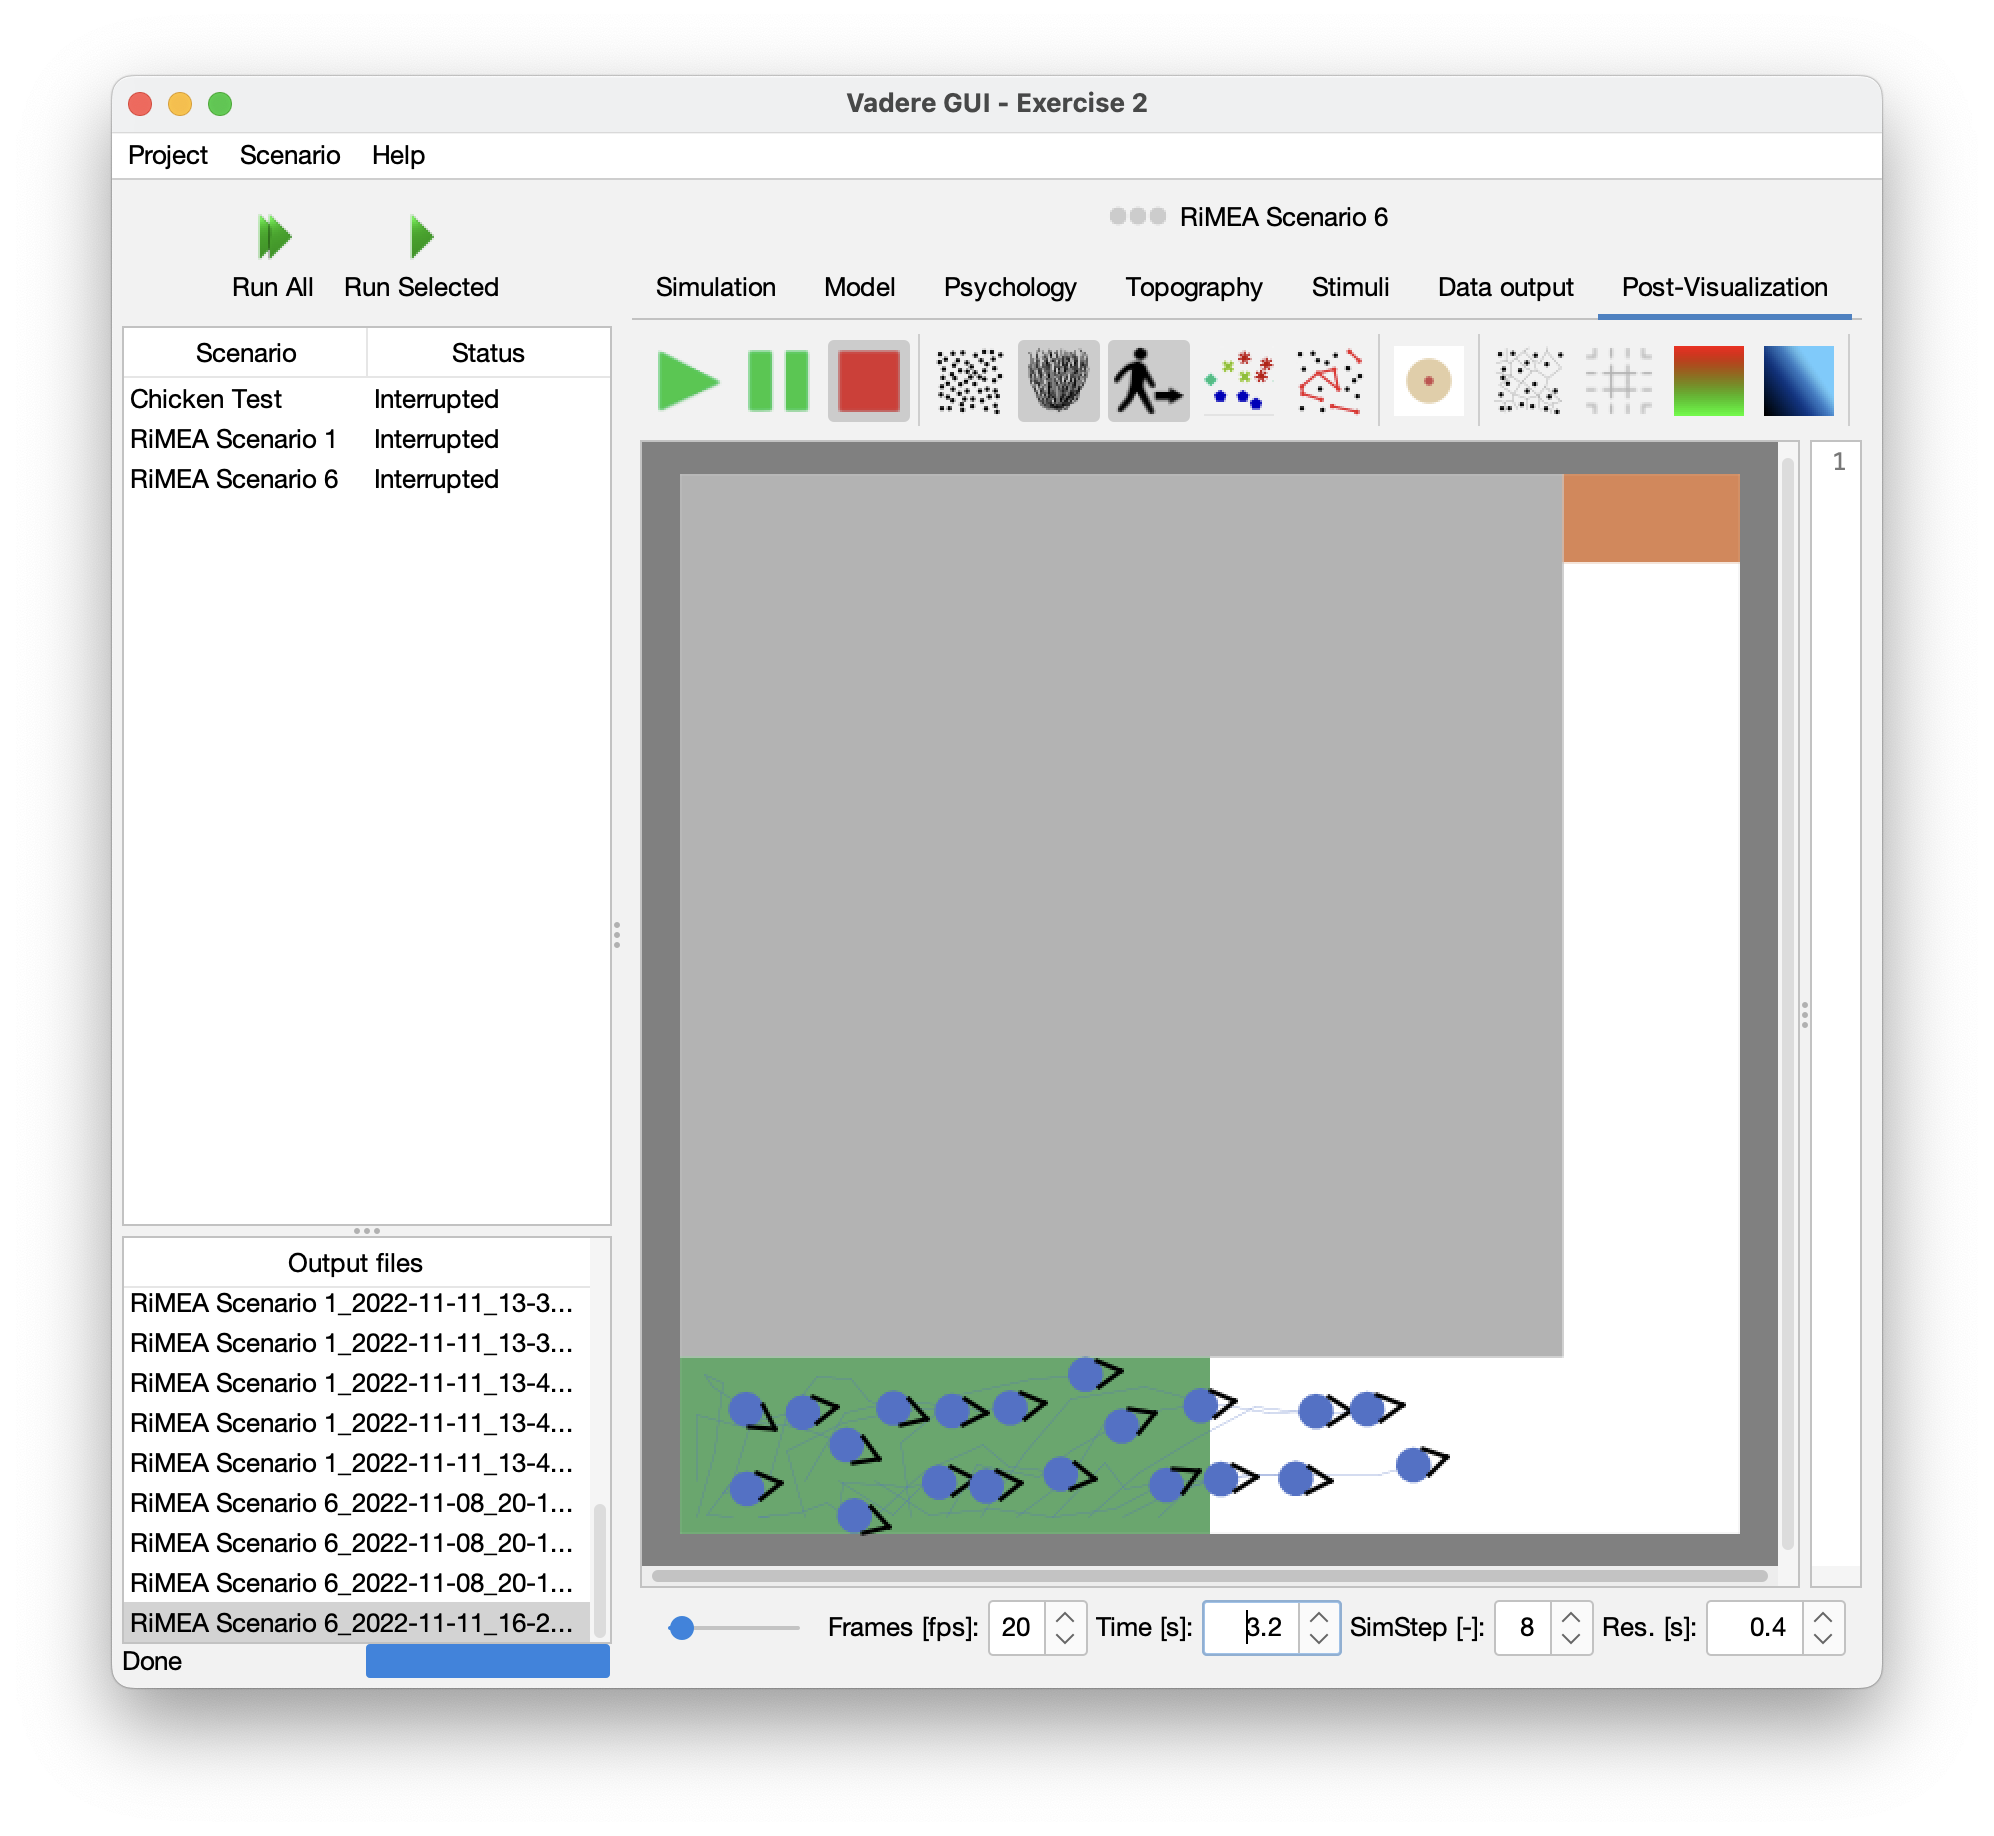
\includegraphics[width=0.33\textwidth]{images/scenario_6a.png}}
  \subfloat[In the middle of the simulation]{
   \label{scenario_6b}
    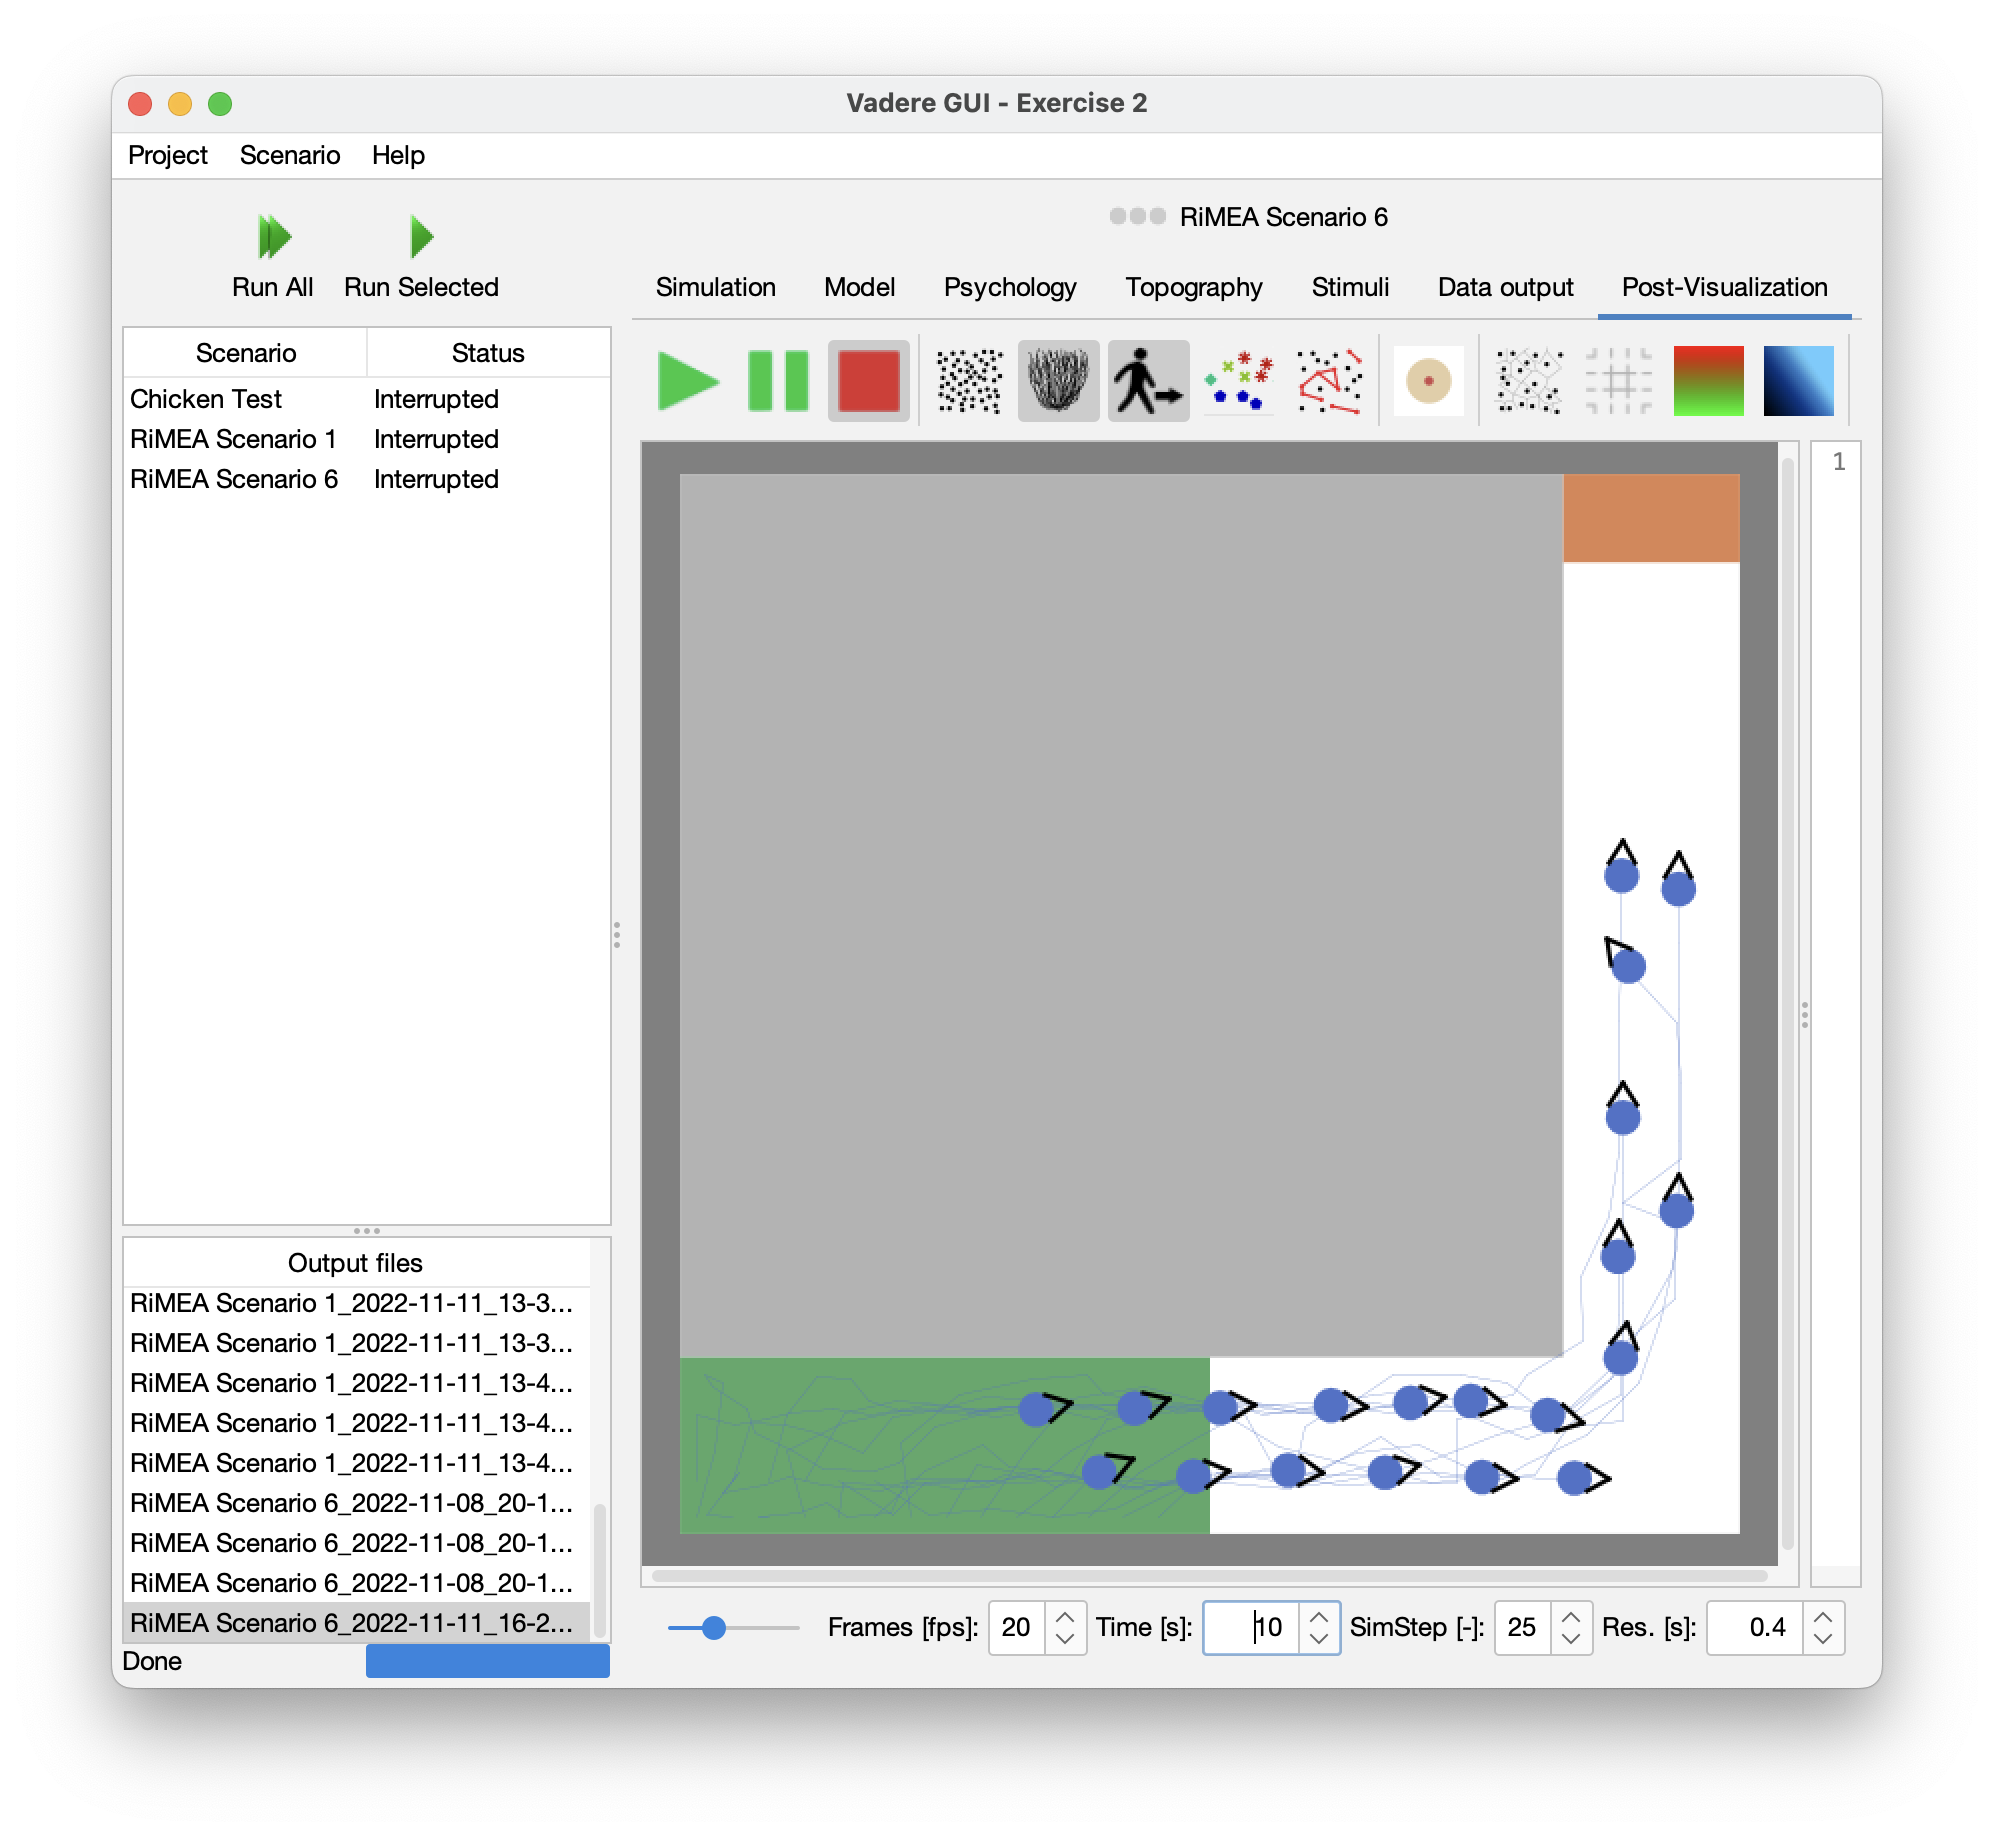
\includegraphics[width=0.33\textwidth]{images/scenario_6b.png}}
  \subfloat[At the end of the simulation]{
   \label{scenario_6c}
    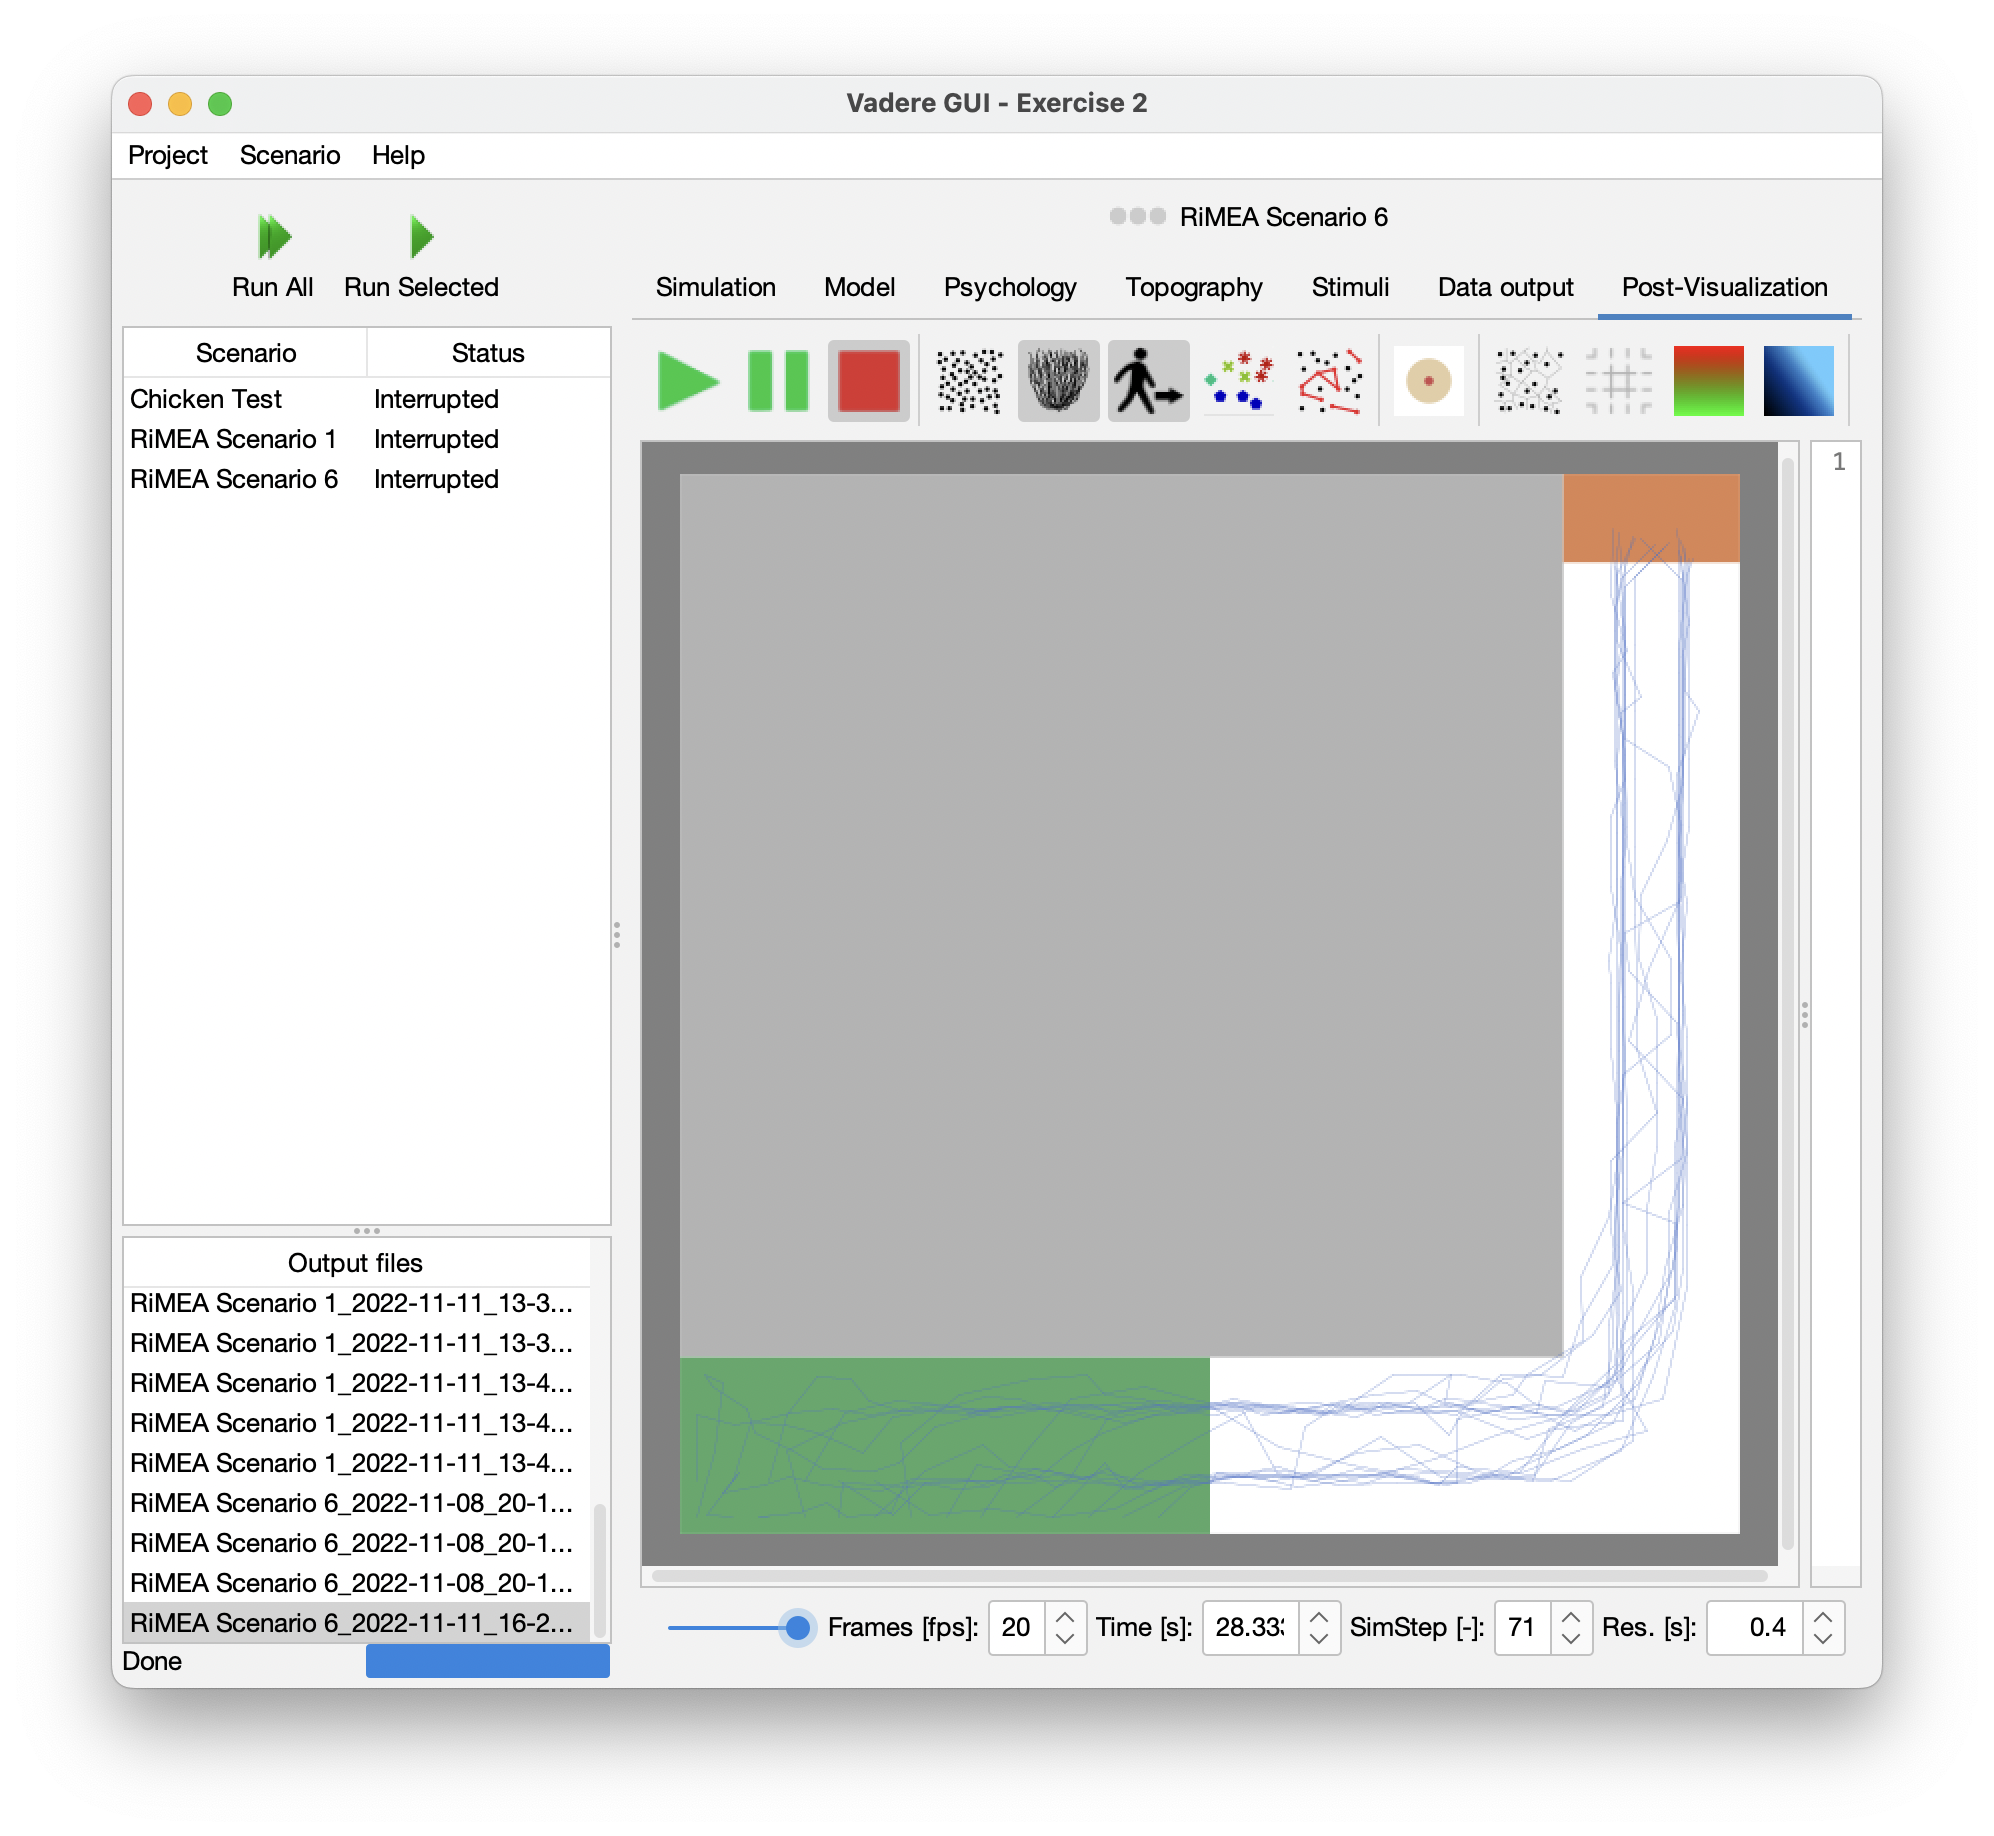
\includegraphics[width=0.33\textwidth]{images/scenario_6c.png}}
 \caption{Different stages of the simulation of the scenario 6}
 \label{scenario6_sim}
\end{figure}

\clearpage

\noindent{\textbf{Chicken test}}

The chicken test consists in a scenario with pedestrians in one side and their target in the other, with a U-shaped obstacle in the middle obstructing the straight path between them. The point of this simulation is testing whether the pedestrians can avoid the obstacles and reach the target or they get stuck at some point and cannot reach any target.

This scenario has been created with the Vadere environment as shown in Figure \ref{chicken_a}. And the scenario is composed by a set of obstacles forming a vertical U shape and the pedestrians placed in 3 different places: outside, at the beginning and inside of the U form obstacles. The target is placed at the same level of the pedestrians, so in the case there weren't obstacles, the optimal path for the pedestrians to reach the target is a straight line, but since there are obstacles, pedestrians cannot follow the straight line path so they have to flip the U form obstacles and then reach the target.

As it can be seen in the Figure \ref{chicken_c}, all the pedestrians from the different places have reached to the target turning around the U-shaped obstacle.

Comparing the results with those obtained in the cellular automaton of exercise 1, the pedestrians have roughly the same behaviour if the algorithm chosen in the exercise 1 is Dijkstra or the Fast Marching Method. If the basic algorithm is chosen in the exercise 1, the pedestrians does not perform in the same way, since in the basic algorithm is not implemented the obstacle avoidance, and therefore the pedestrians get stuck in the U-shaped obstacle.

\begin{figure} [H]
 \centering
  \subfloat[At the beginning of the simulation]{
   \label{chicken_a}
    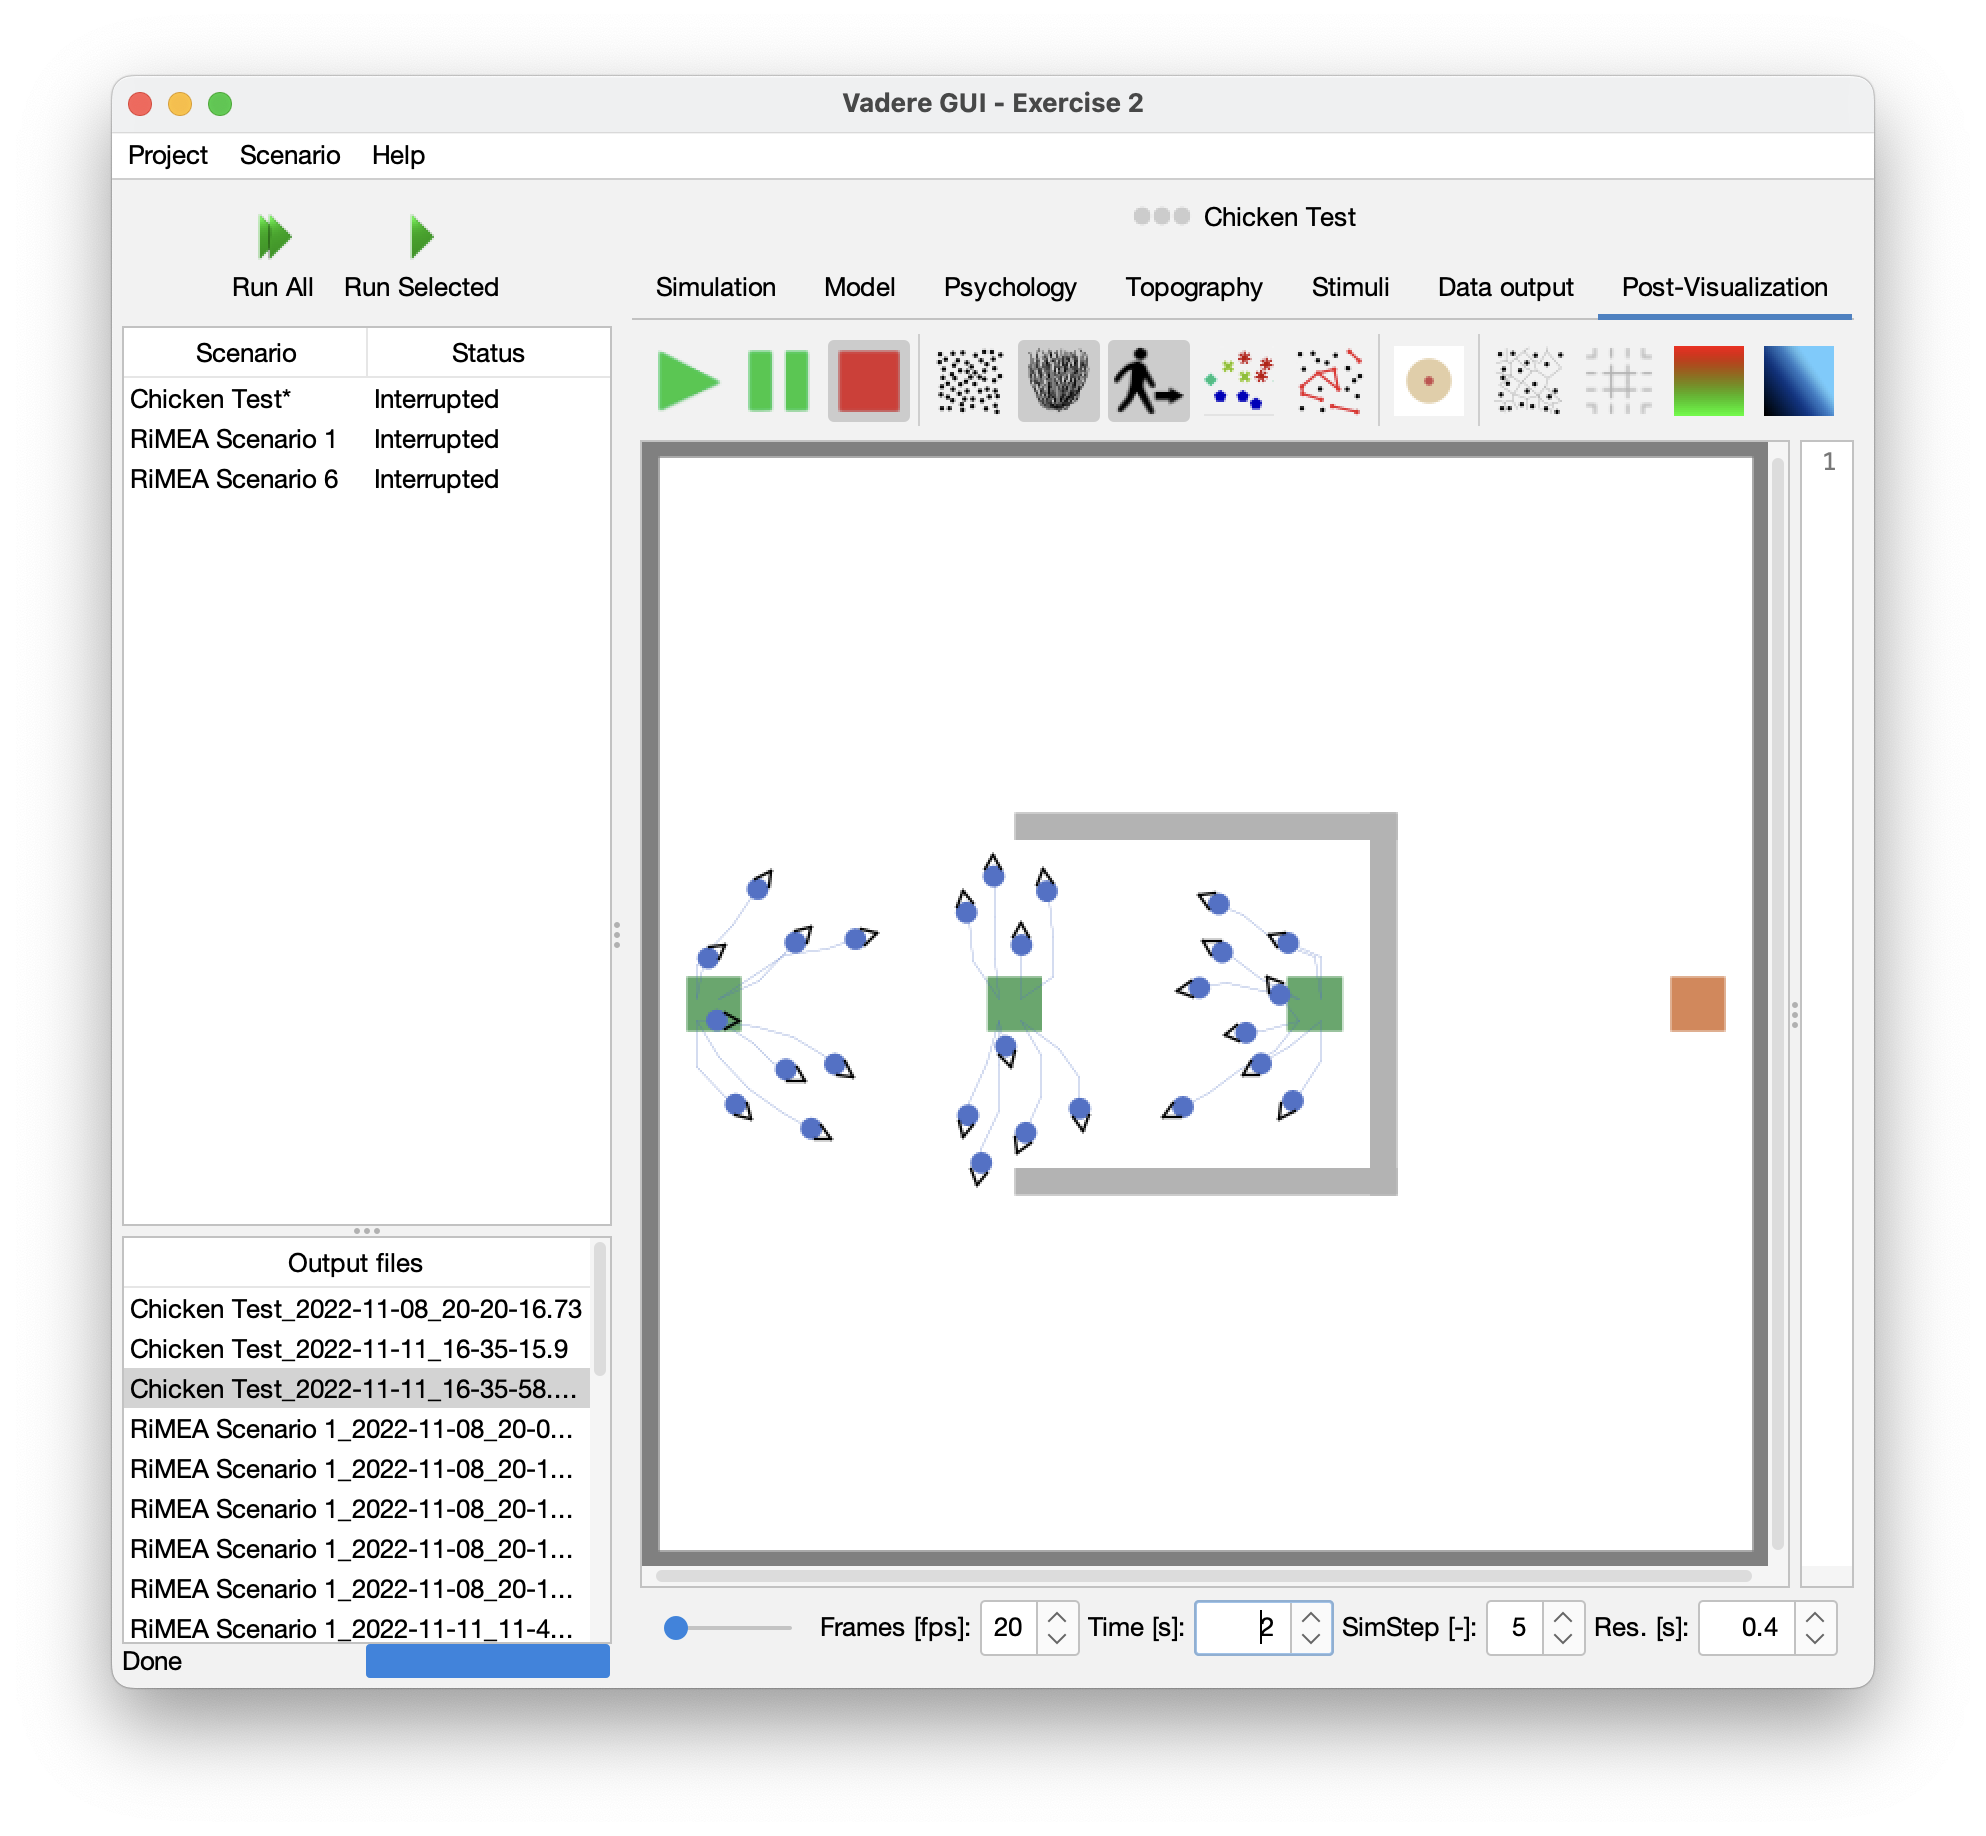
\includegraphics[width=0.33\textwidth]{images/chicken_a.png}}
  \subfloat[In the middle of the simulation]{
   \label{chicken_b}
    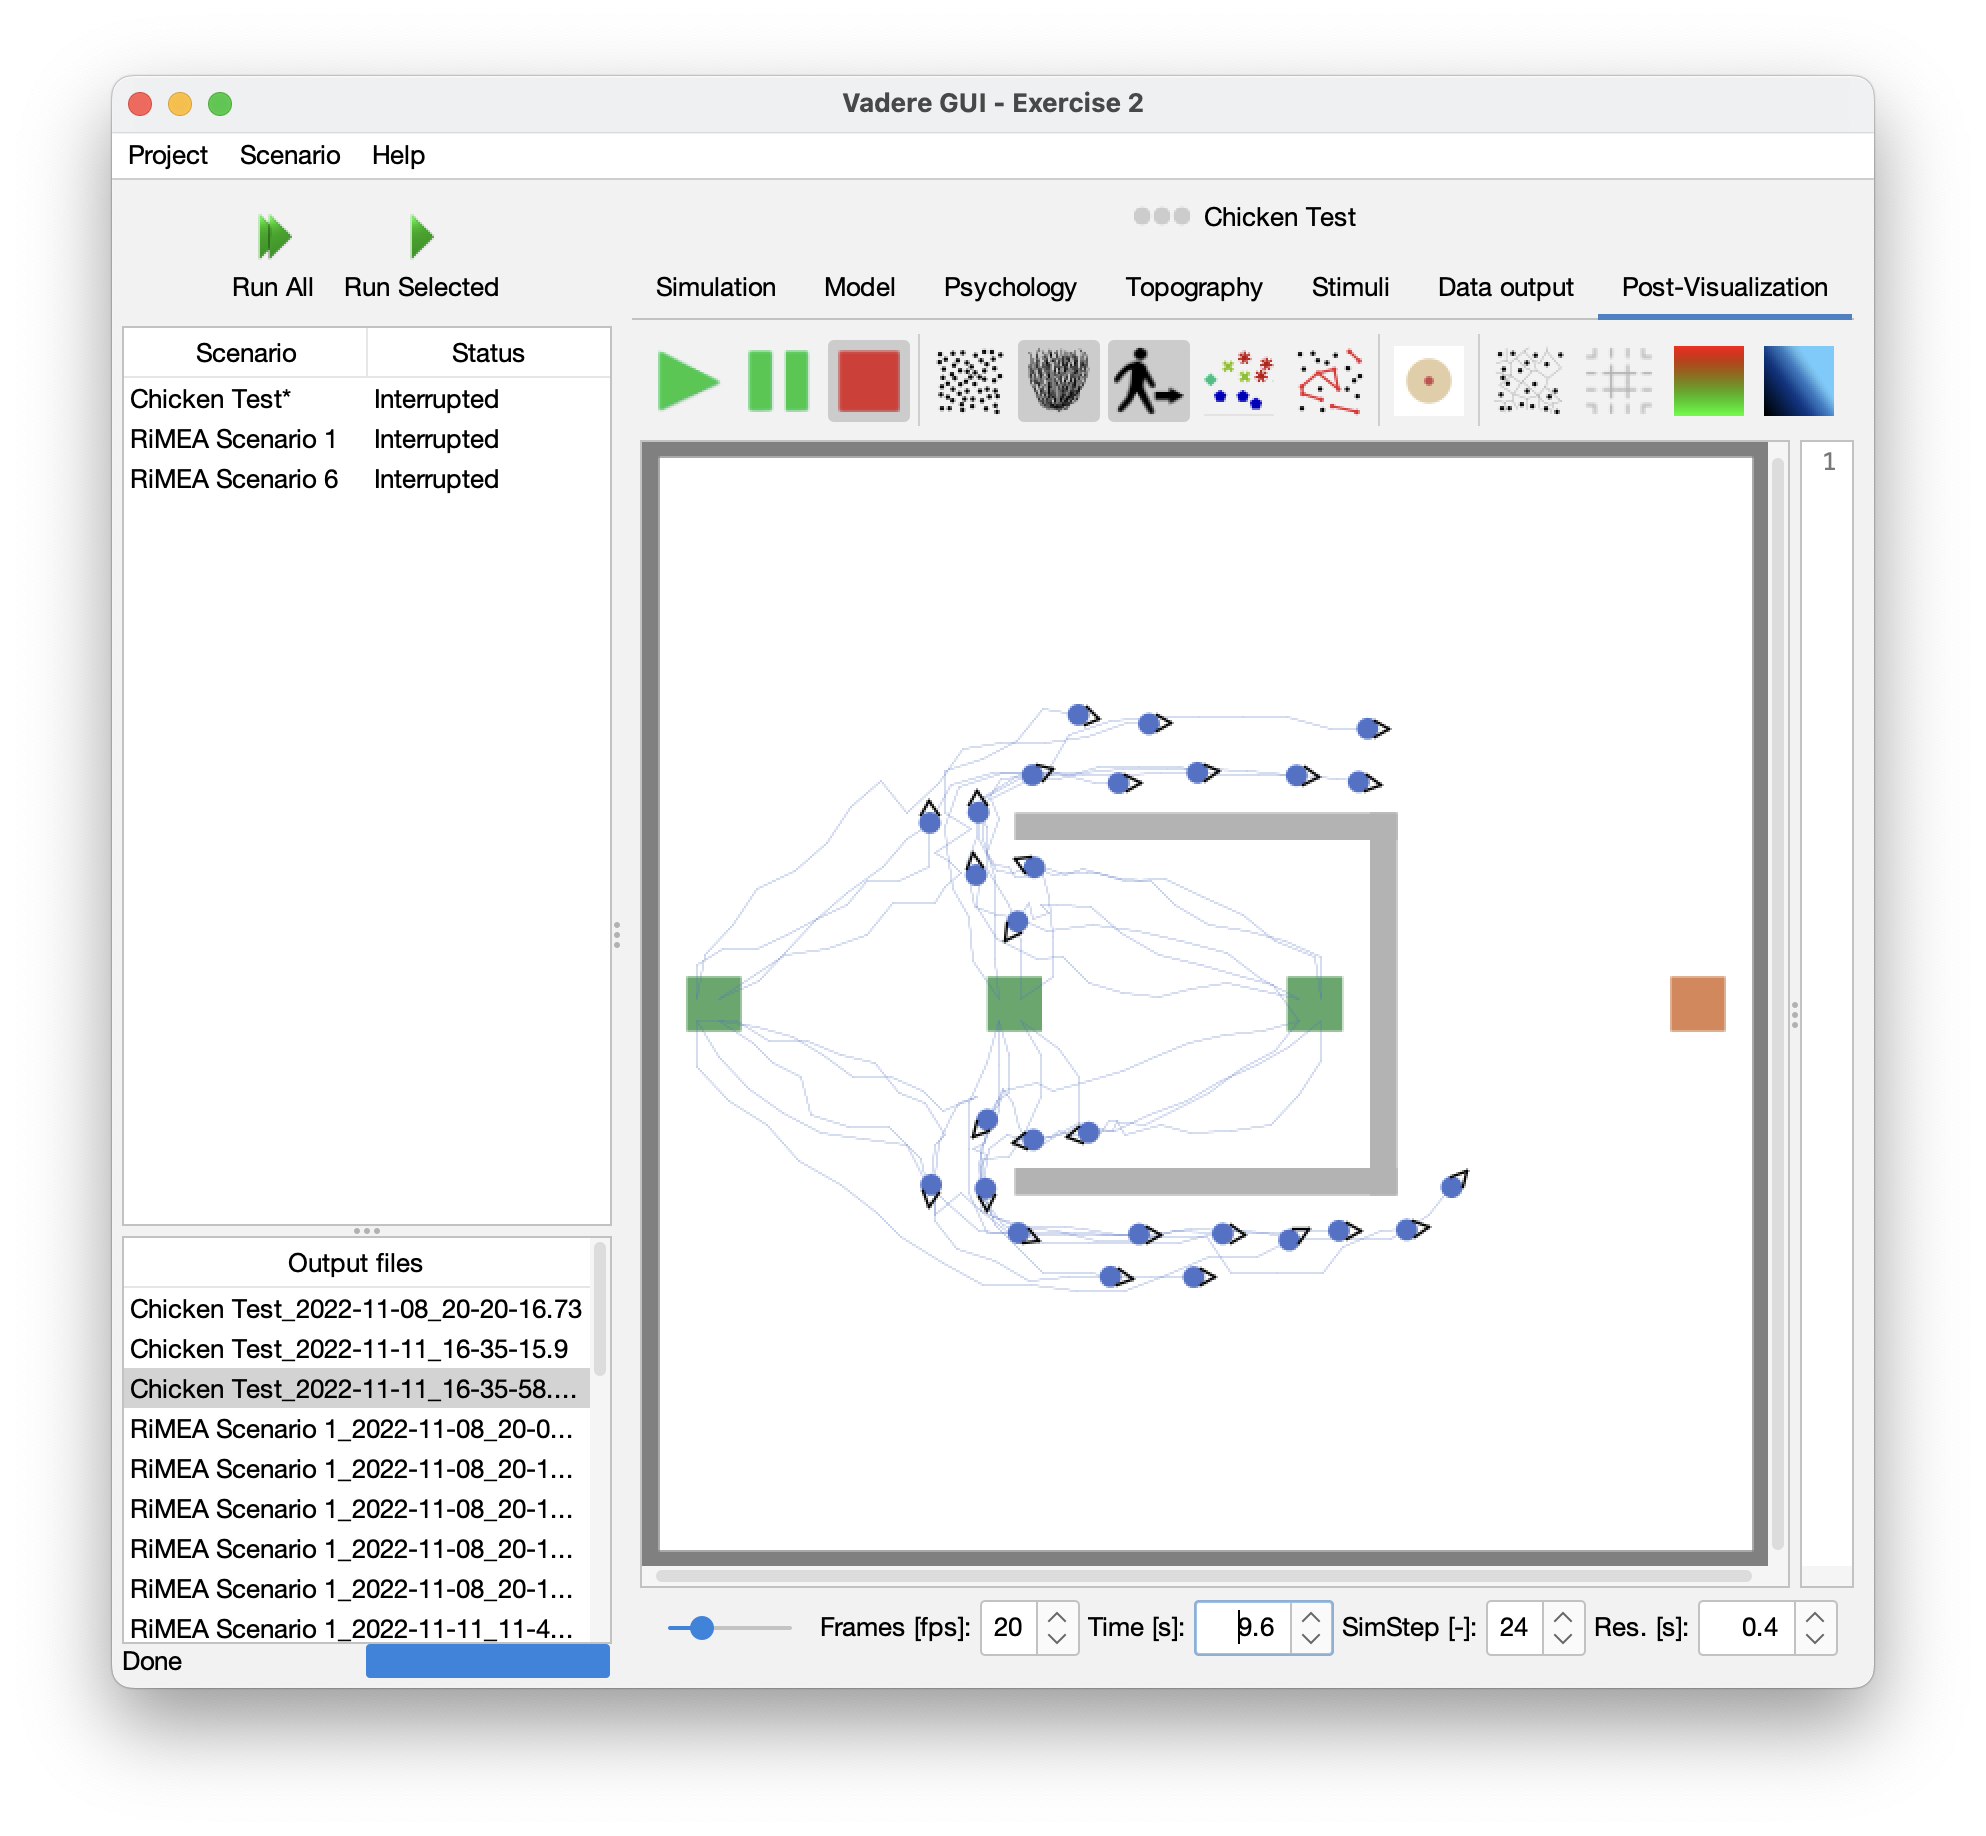
\includegraphics[width=0.33\textwidth]{images/chicken_b.png}}
  \subfloat[At the end of the simulation]{
   \label{chicken_c}
    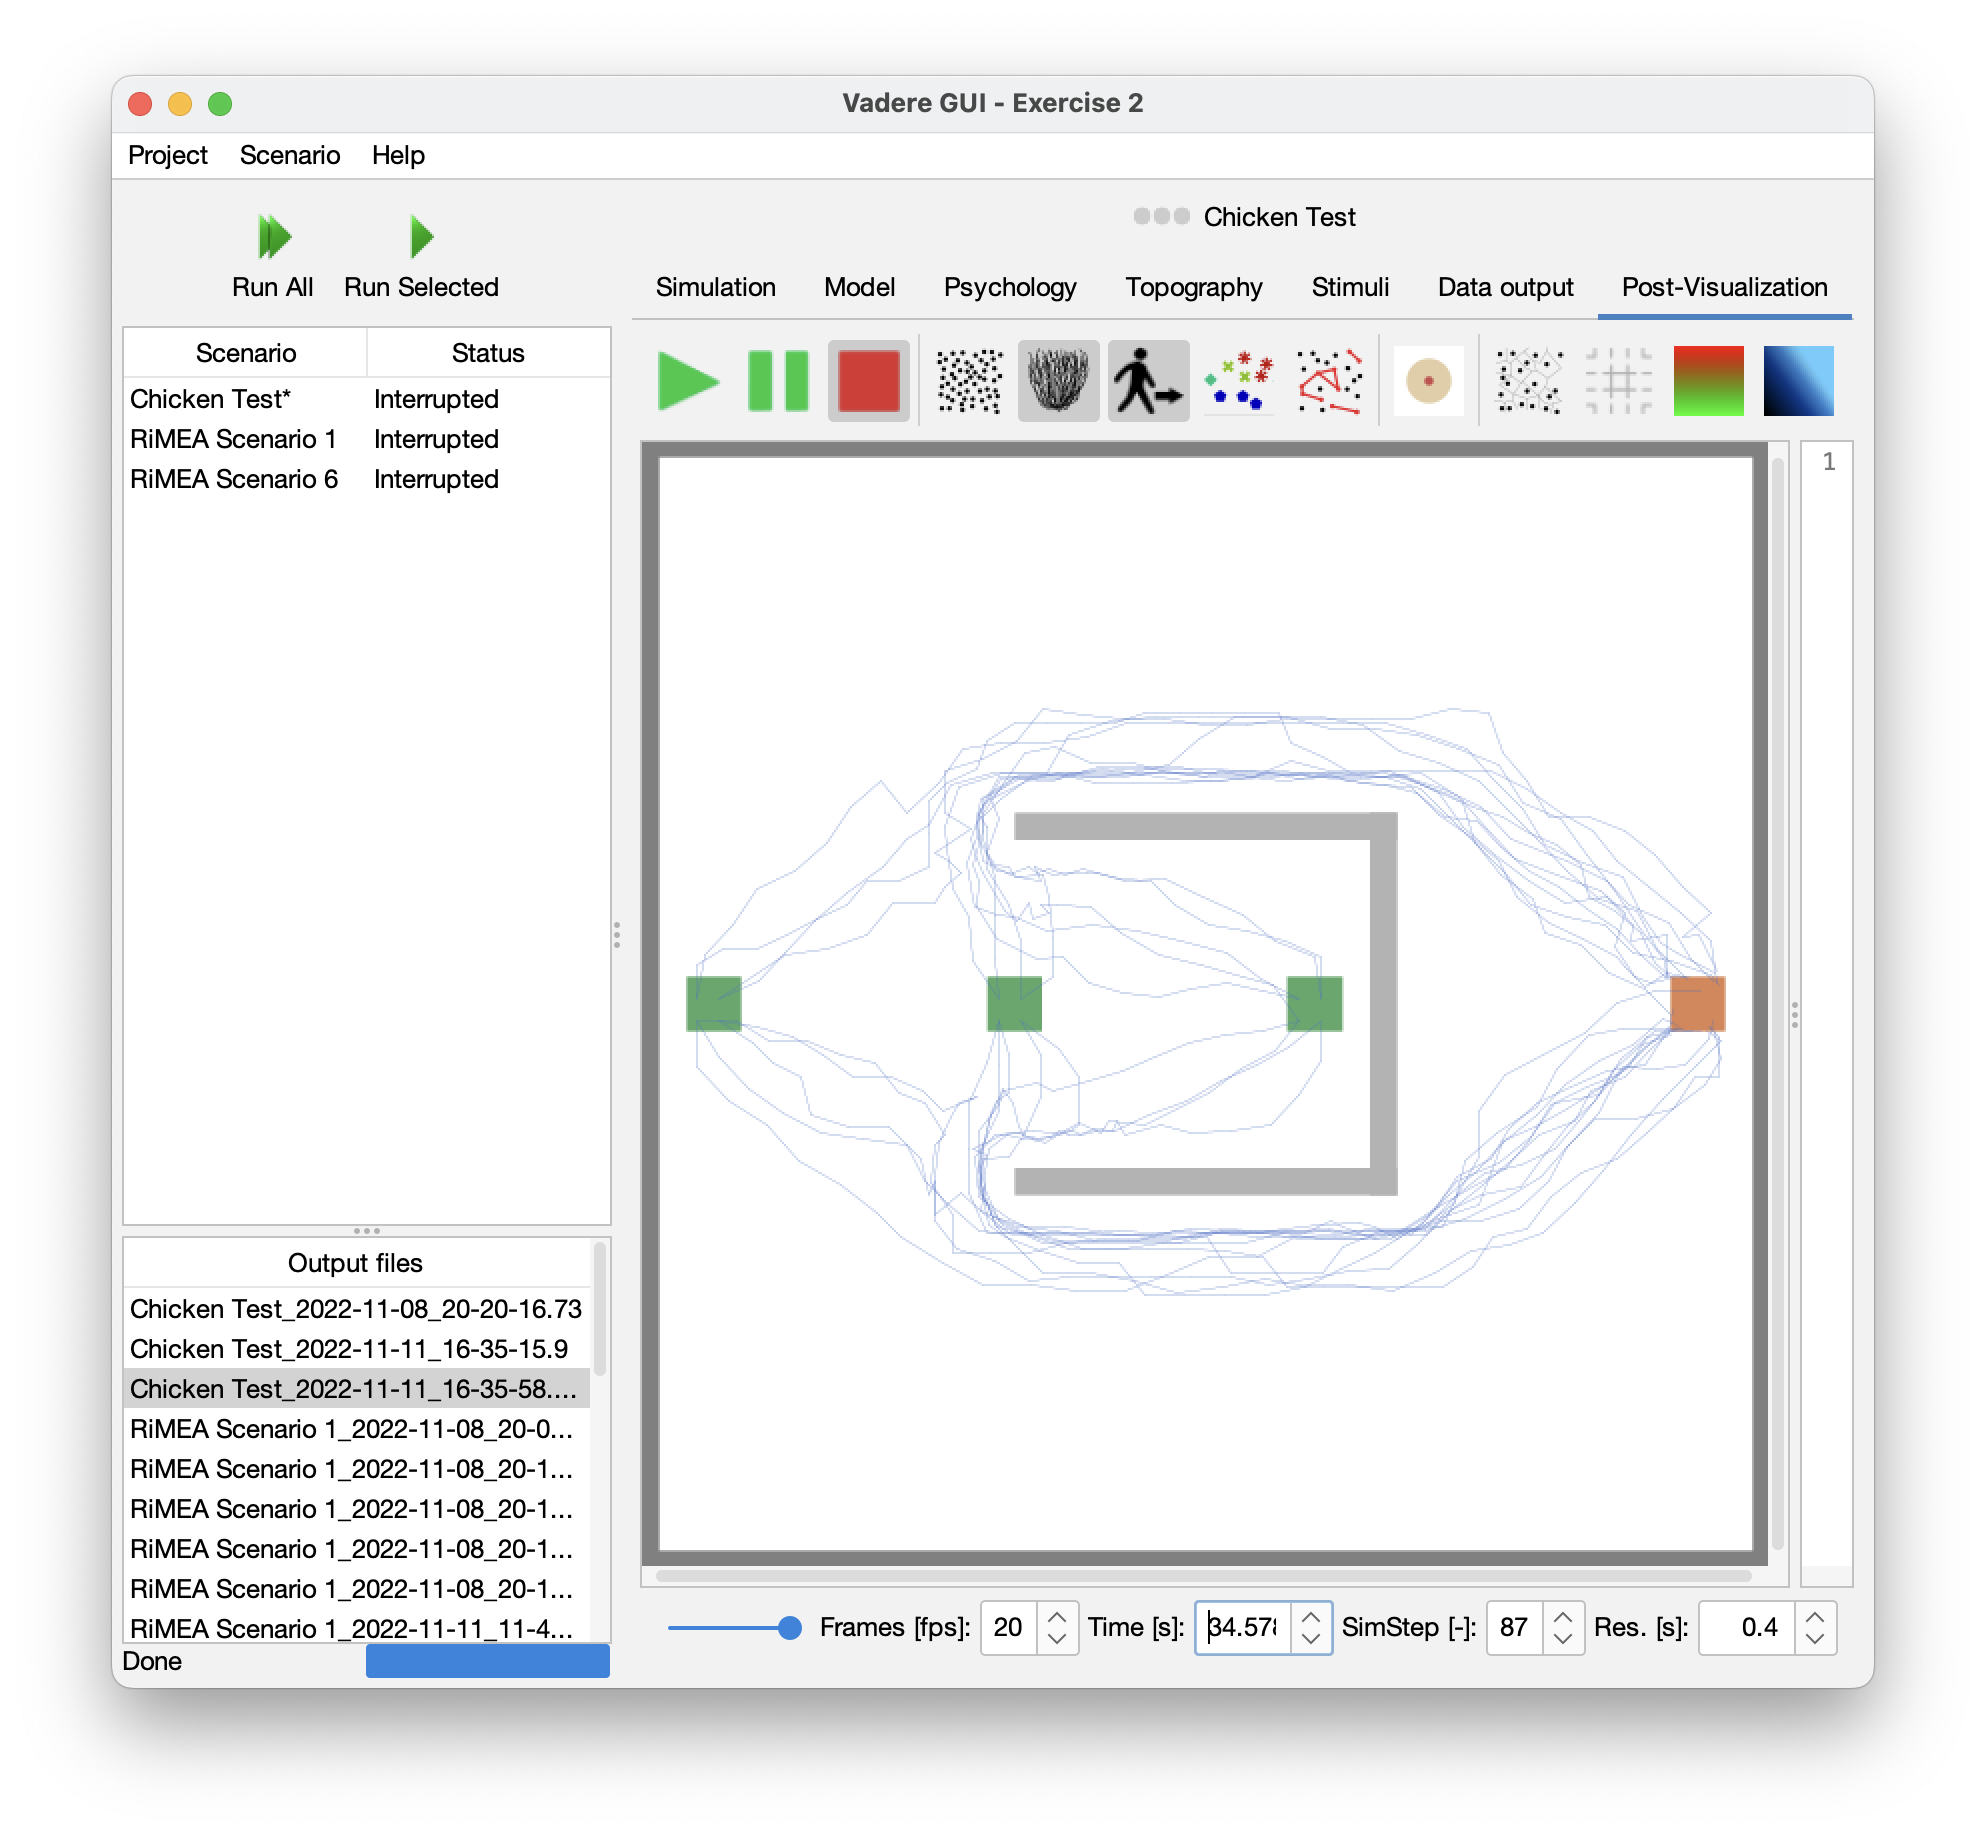
\includegraphics[width=0.33\textwidth]{images/chicken_c.png}}
 \caption{Different stages of the simulation of the chicken test}
 \label{chicken_sim}
\end{figure}


\end{task}

\clearpage

\begin{task}{2, Simulation of the scenario with a different model}

In this task, the three scenarios from the previous task will be re-run with other two different models: the Social Force Model and the Gradient Navigation Model. Both models will be compared to the Optimal Steps Model, the one used in the previous task, and the differences and similarities observed during the simulations will be analysed and reported in the following subsections. At the end, a joint analysis will be done for all three models.

\bigskip

\noindent{\textbf{Social Force Model (SFM)}}

\begin{enumerate}[label=(\alph*)]
    \item RiMEA scenario 1: in this first case, with Social Force Model the pedestrian does not follow a straight line path anymore, instead, as we can see in the Figure \ref{sfm_1c}, it moves downwards 3 positions in the first half of the simulation and later it goes up 1 position before reaching the target. With Optimal Step Model, the pedestrian follows a straight line path to reach the target. The travel time in both simulations are nearly the same (30 s with SFM and 30,57 s with OSM). As they behave nearly in the same way and it is a very simple scenario, it is hard to know why the SFM does not follow a strictly  
    straight line.
    
    \begin{figure} [H]
    \centering
    \subfloat[At the beginning of the simulation]{
        \label{sfm_1a}
        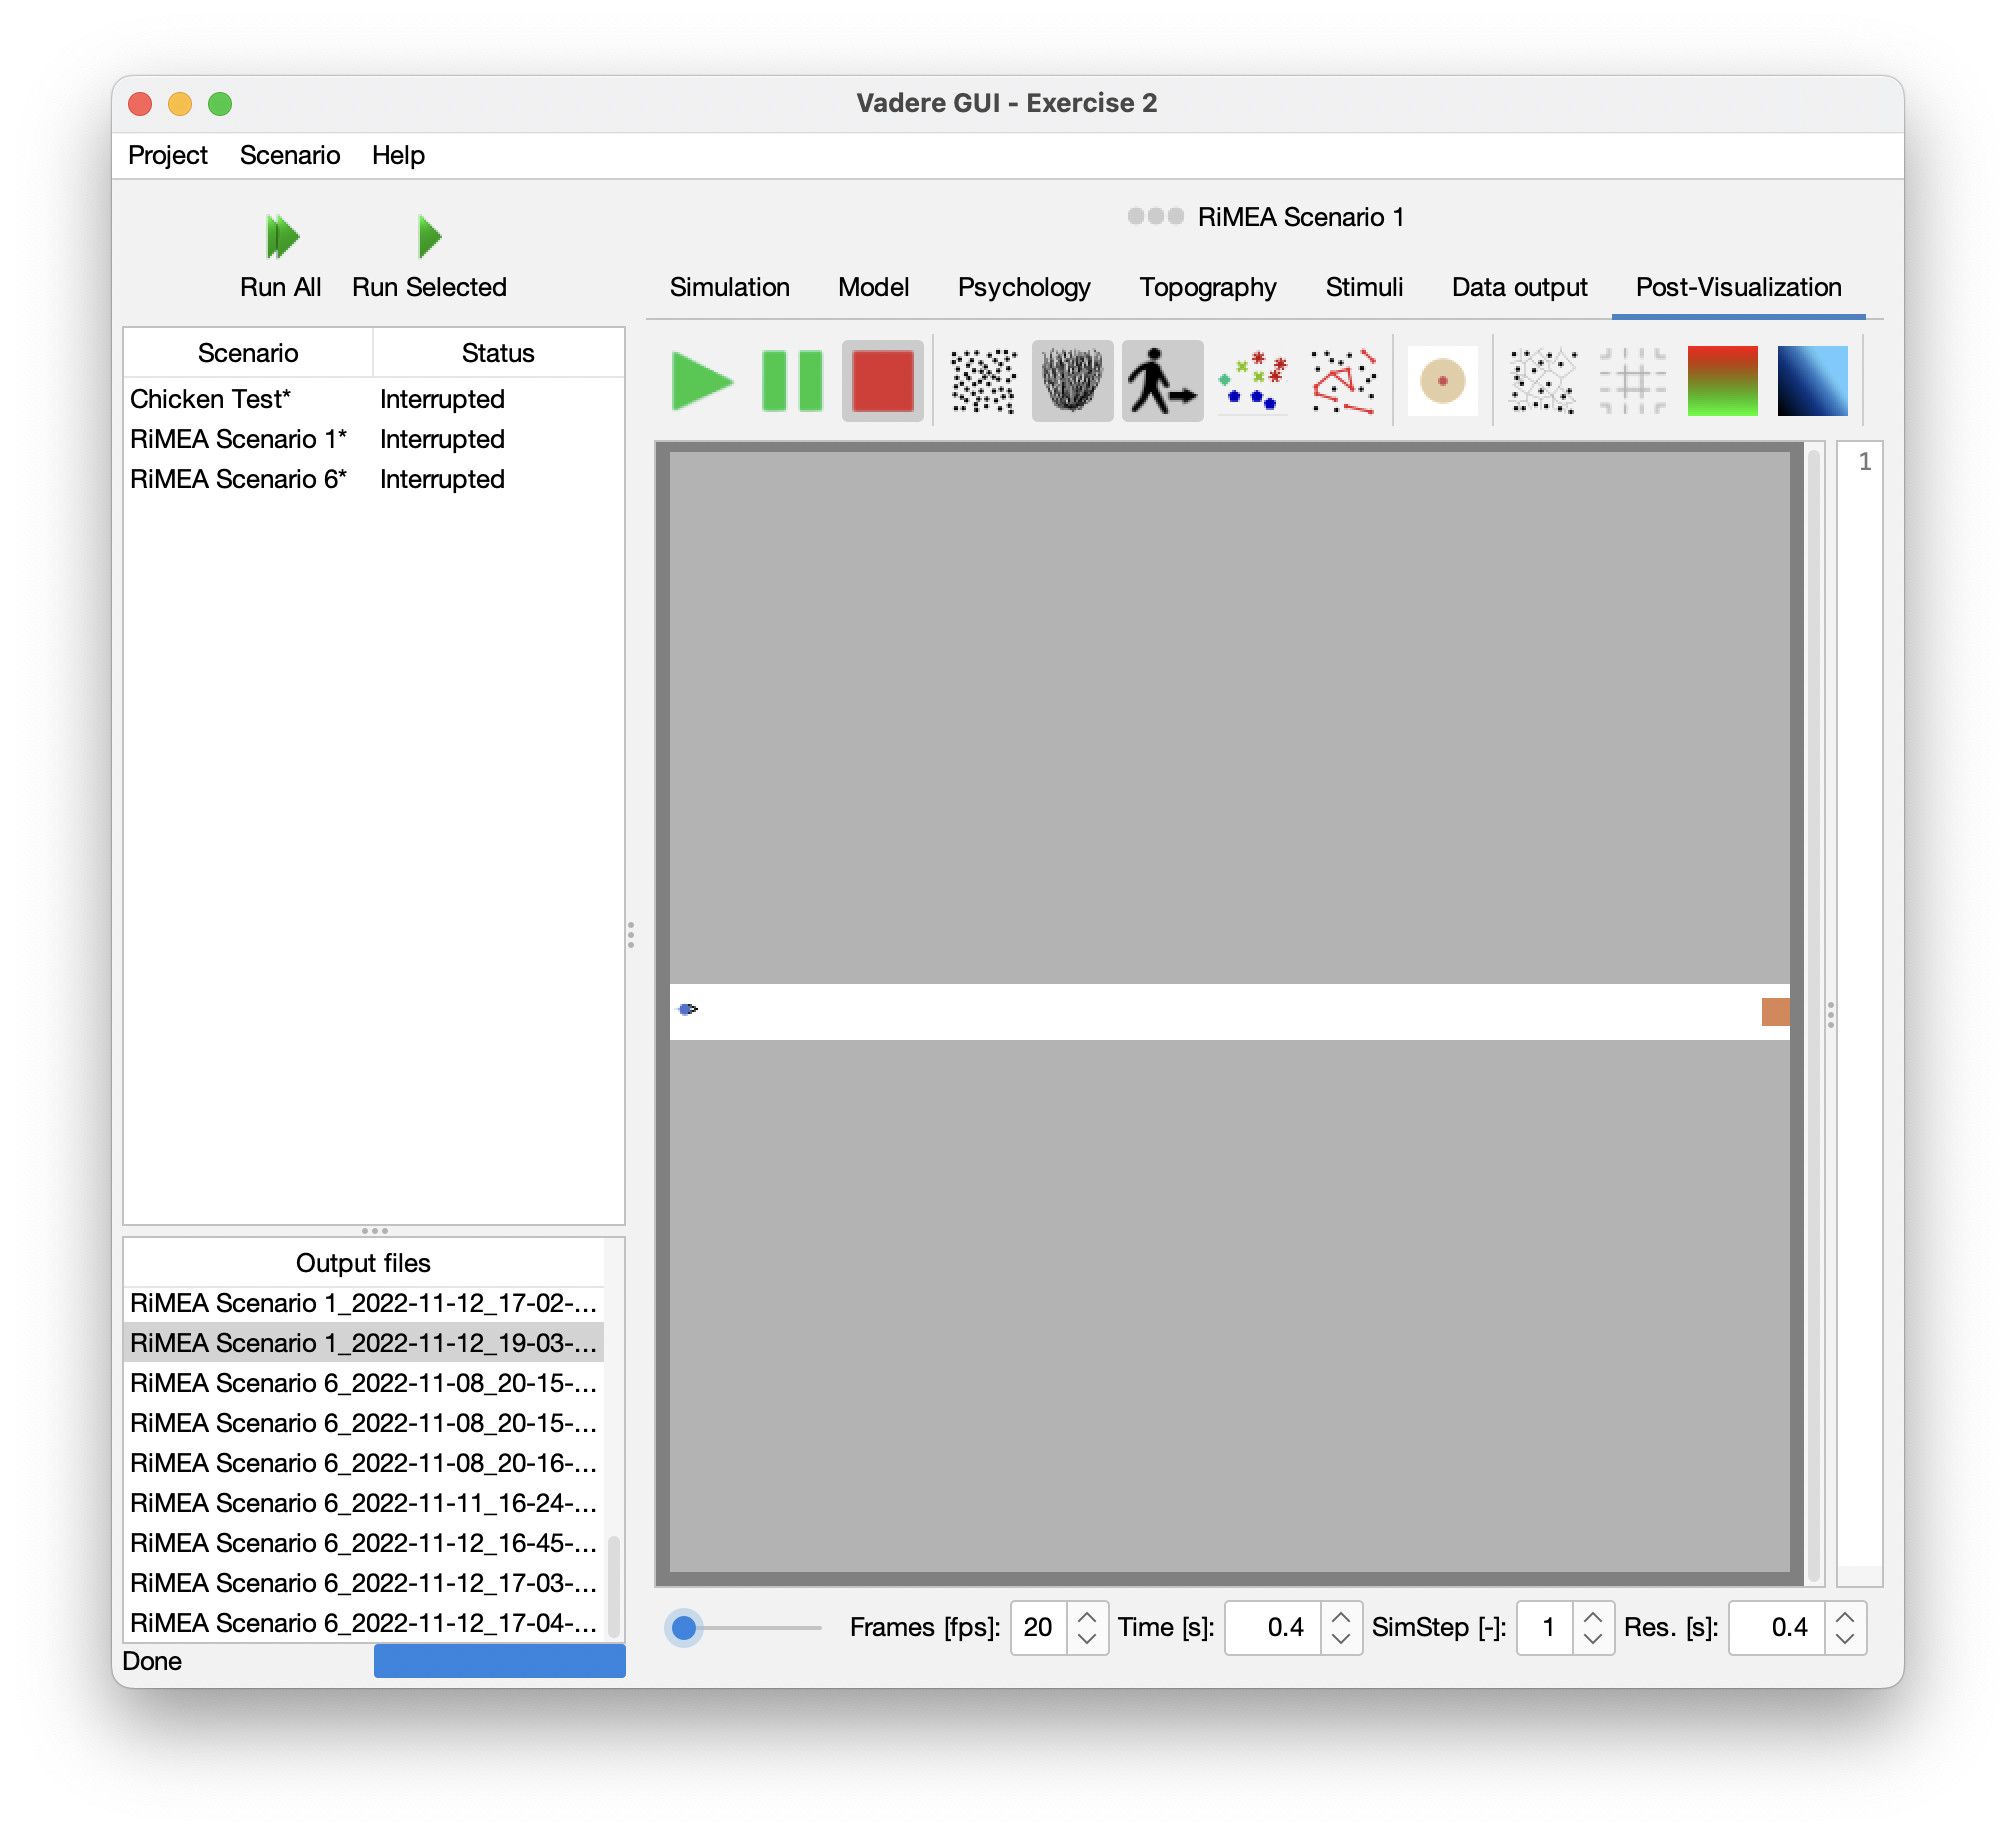
\includegraphics[width=0.33\textwidth]{images/sfm_1a.png}}
        \subfloat[In the middle of the simulation]{
        \label{sfm_1b}
        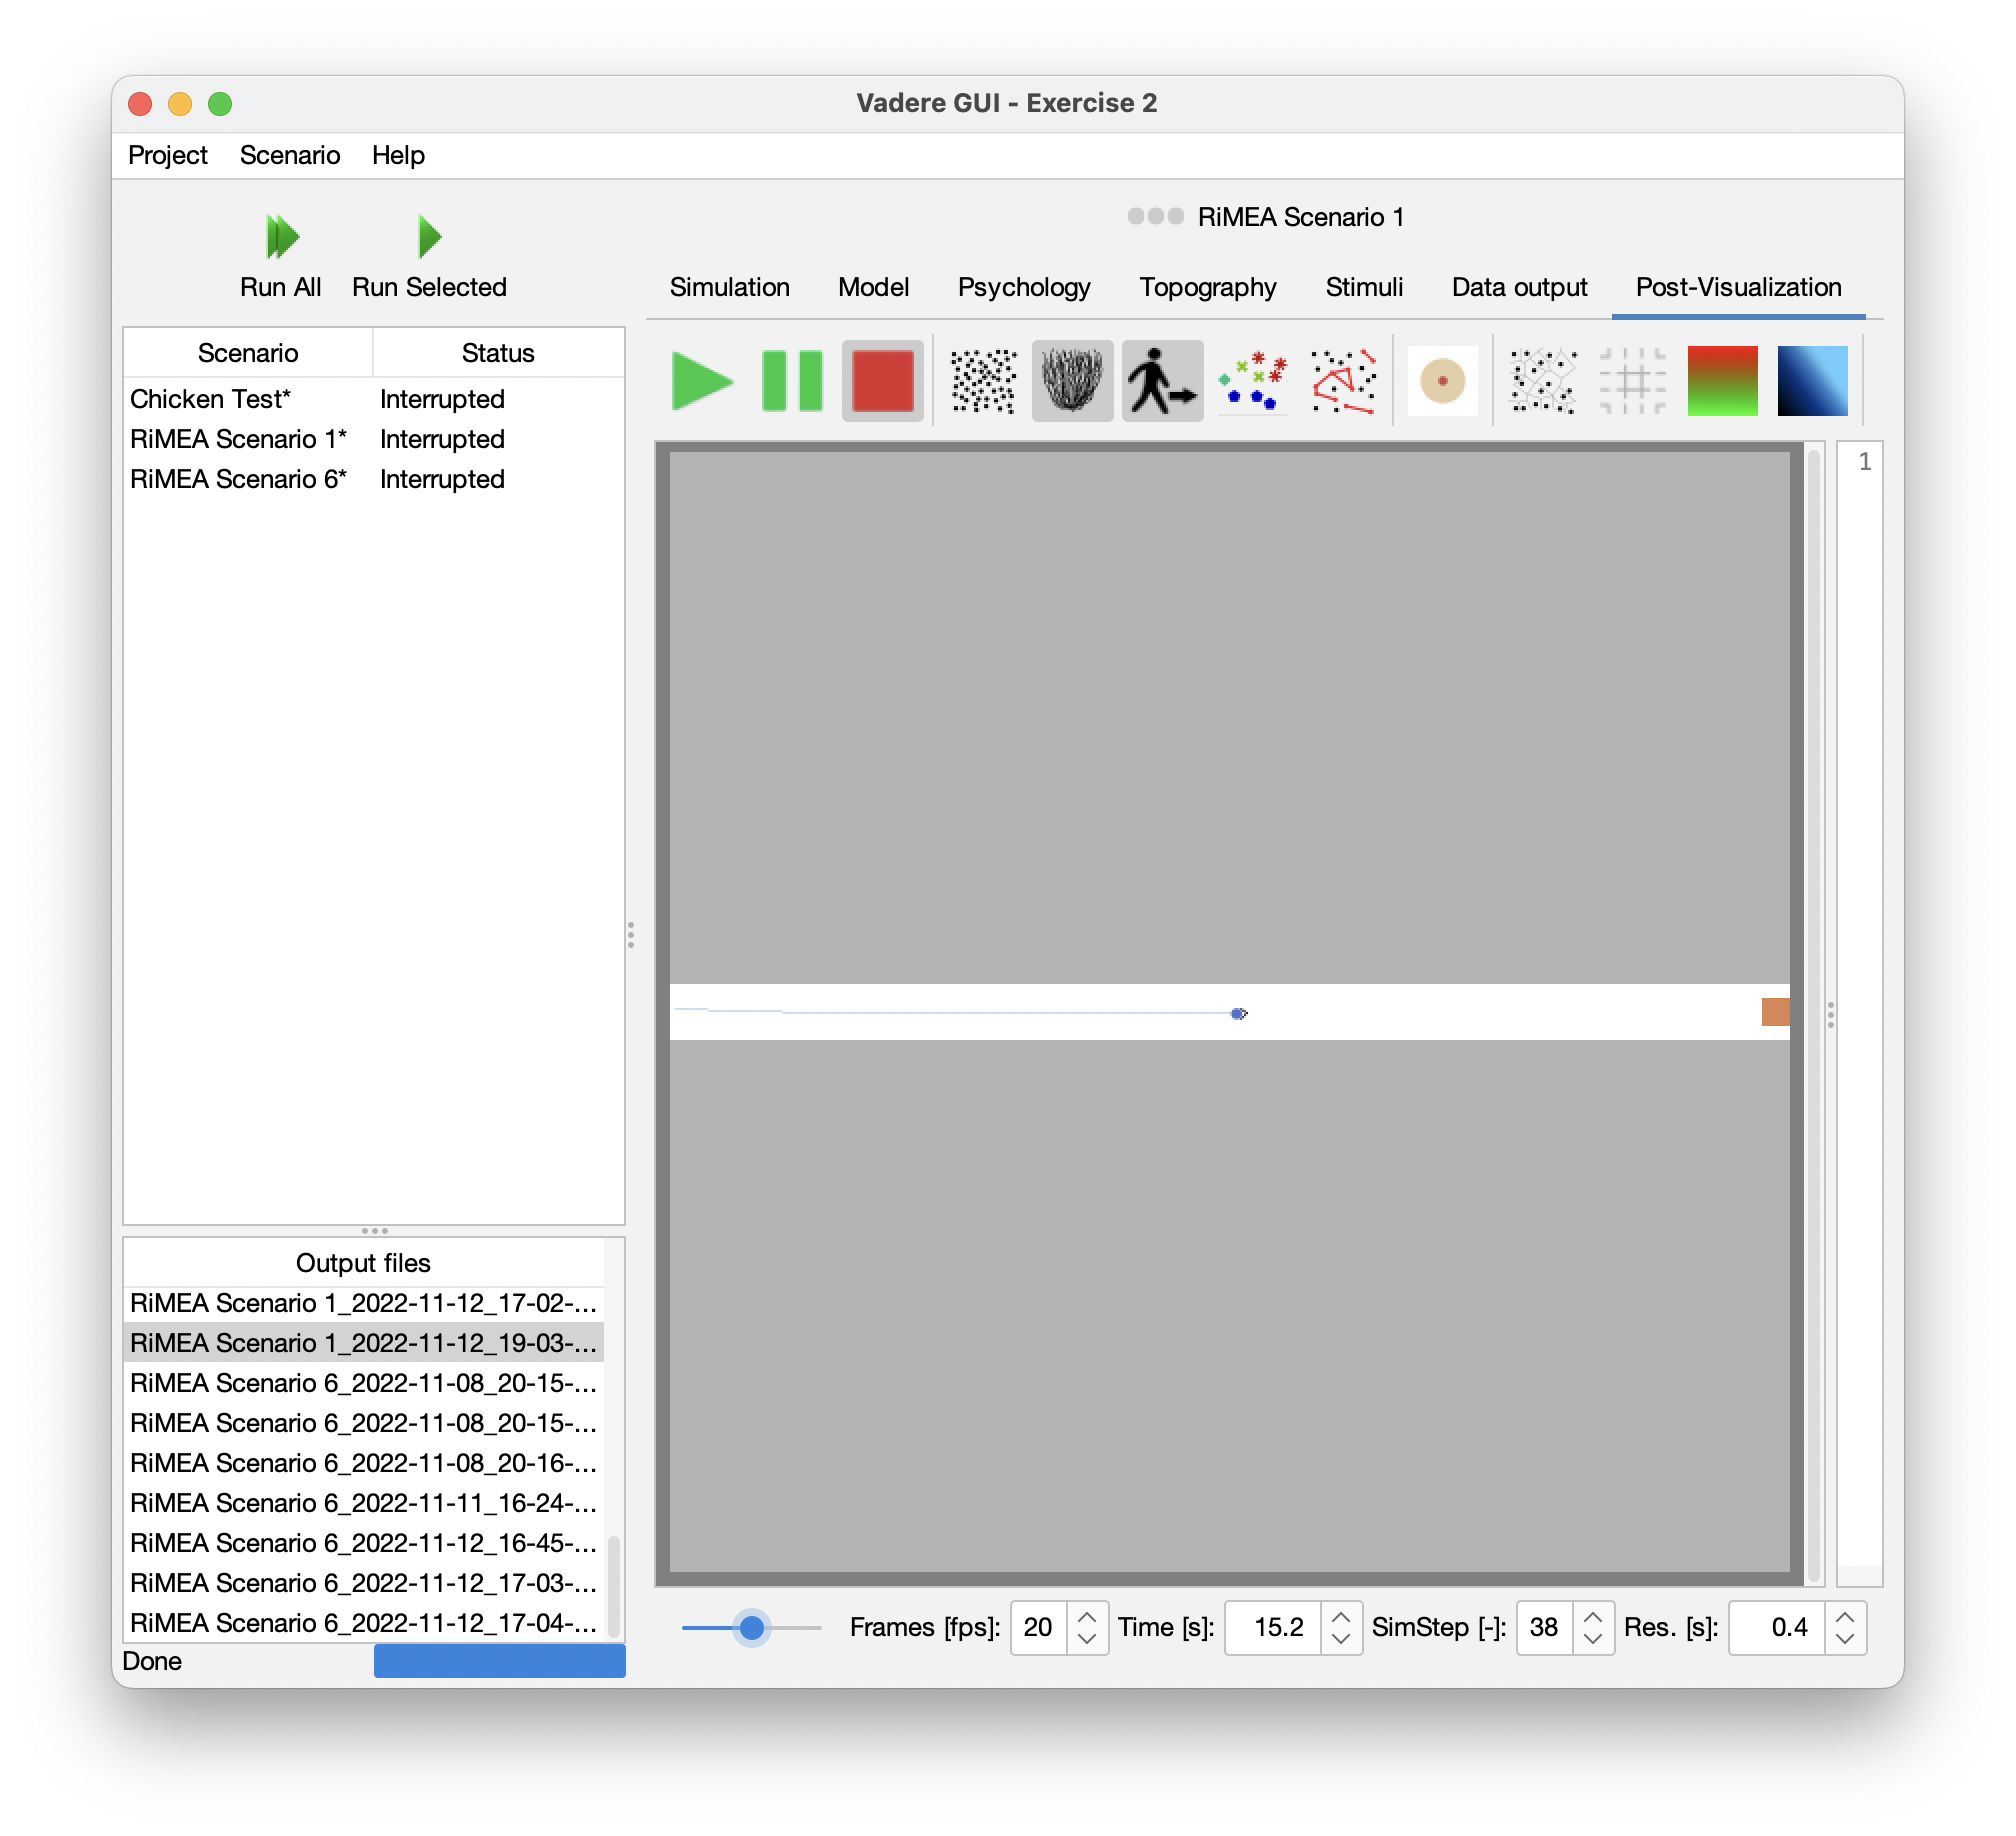
\includegraphics[width=0.33\textwidth]{images/sfm_1b.png}}
        \subfloat[At the end of the simulation]{
        \label{sfm_1c}
        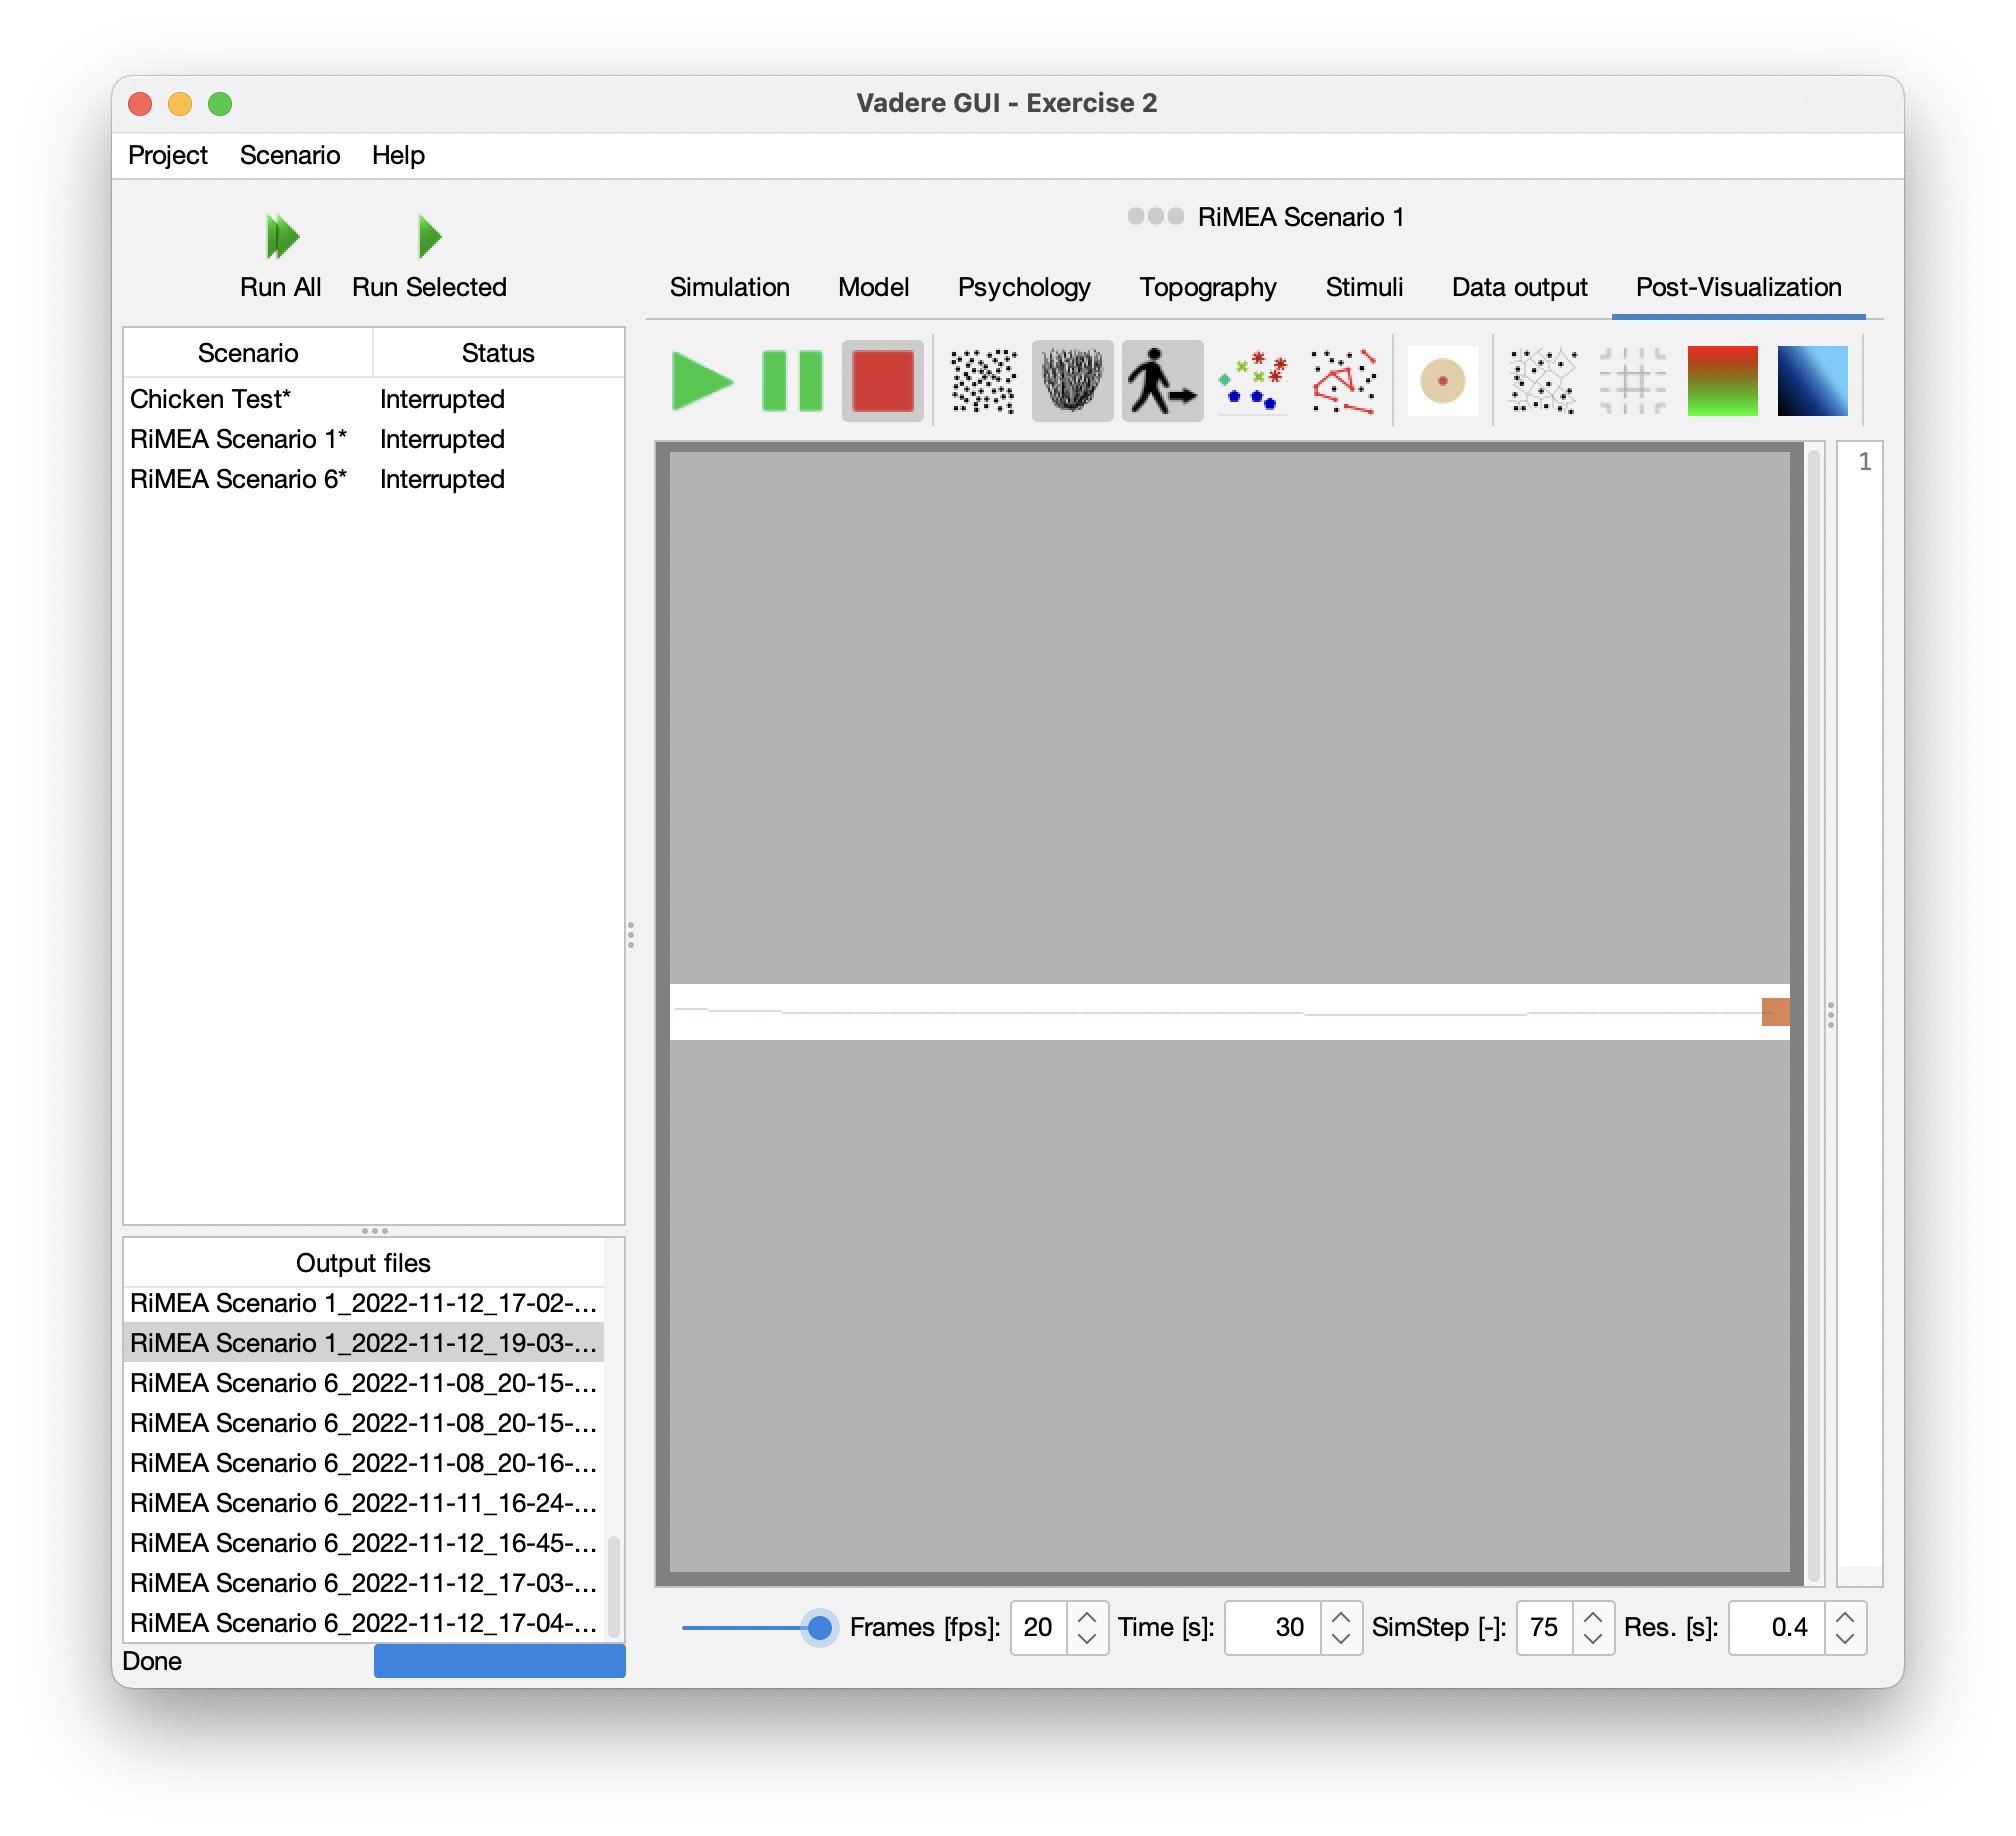
\includegraphics[width=0.33\textwidth]{images/sfm_1c.png}}
        \caption{Different stages of the simulation of the scenario 1 using the Social Force Model}
        \label{scenario1_sfm}
    \end{figure}
    
    
    \item RiMEA scenario 6: with the Social Force Model, the behavior of the pedestrians are more ``ordered" and natural. All the pedestrians tend to follow the optimal/shortest path to reach the target. As we can see in the Figure \ref{sfm_6c}, the paths are more smooths and all of them looks similar to each other and there is a sensation of order, whereas in the Optimal Step Model the paths are a little bit chaotic and pedestrians behaves more ``nervous" trying to reach the target: some of them stops or collide with obstacles at certain point when it is not required. The consequence of that order of the pedestrians can be observed rather on the travel time to the target. It is a little bit faster with the SFM (27.6 s) compared to the OSM (28.33 s). 
    
    \begin{figure} [H]
    \centering
    \subfloat[At the beginning of the simulation]{
        \label{sfm_6a}
        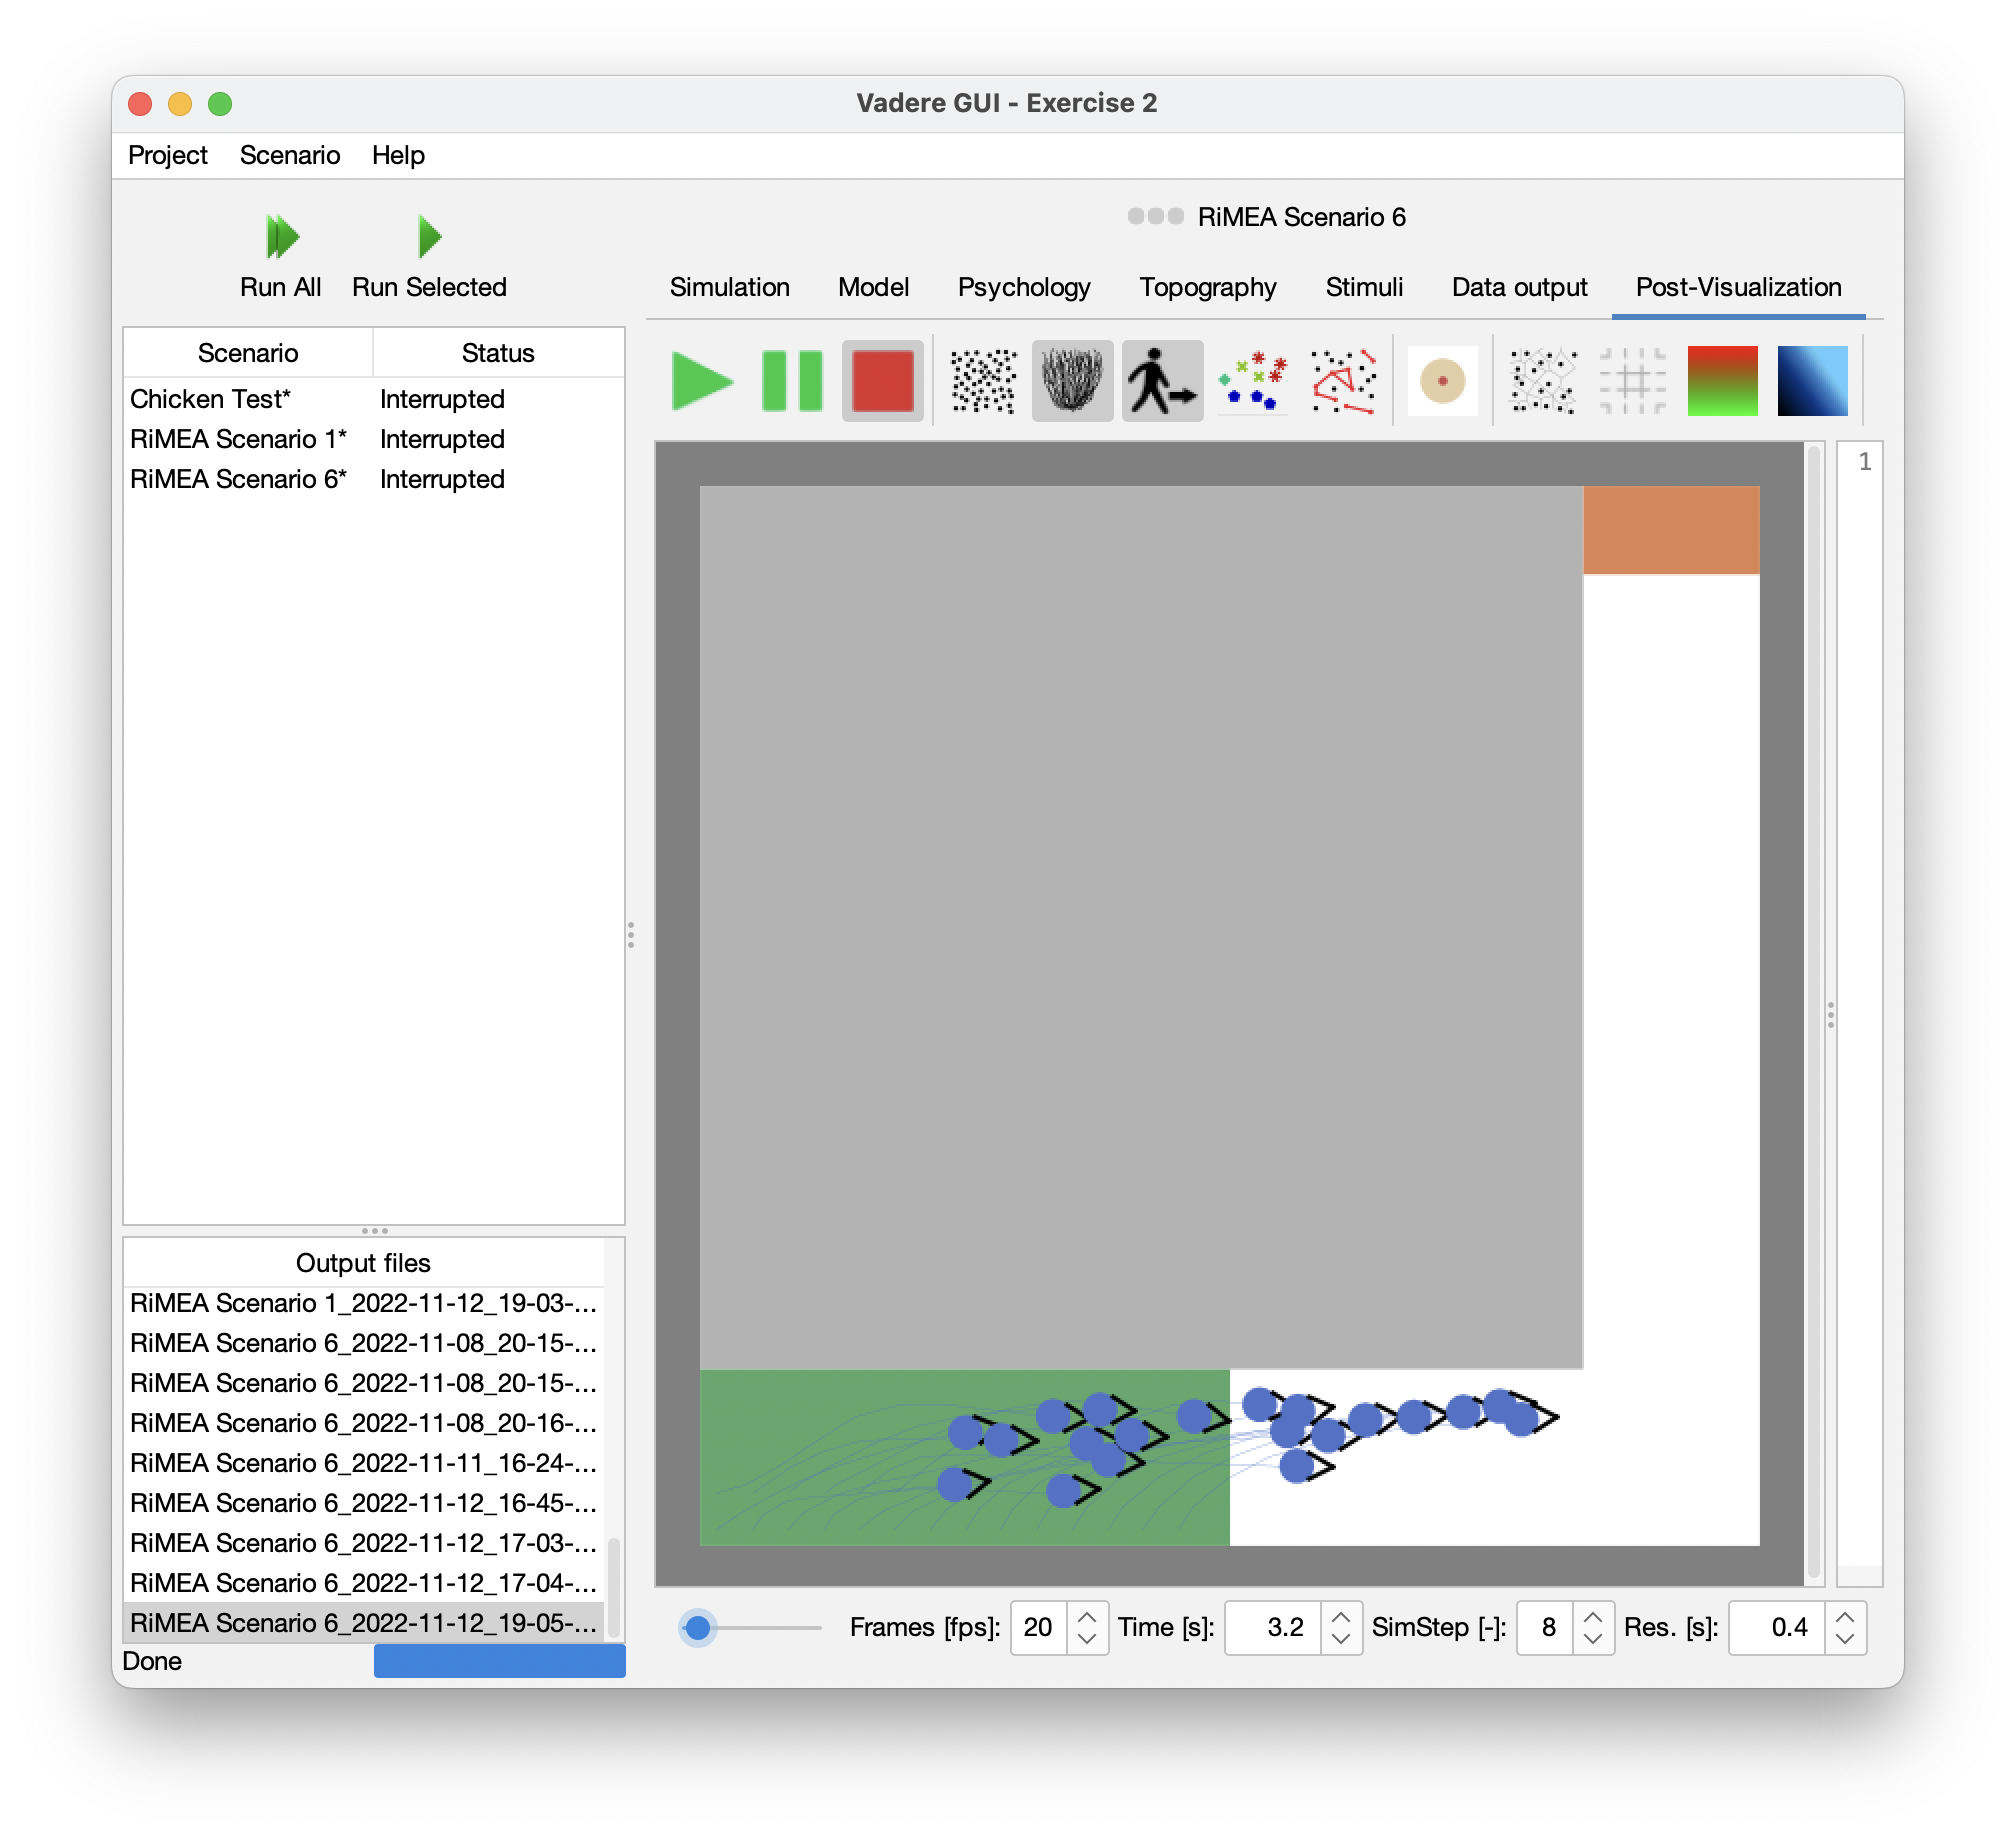
\includegraphics[width=0.33\textwidth]{images/sfm_6a.png}}
        \subfloat[In the middle of the simulation]{
        \label{sfm_6b}
        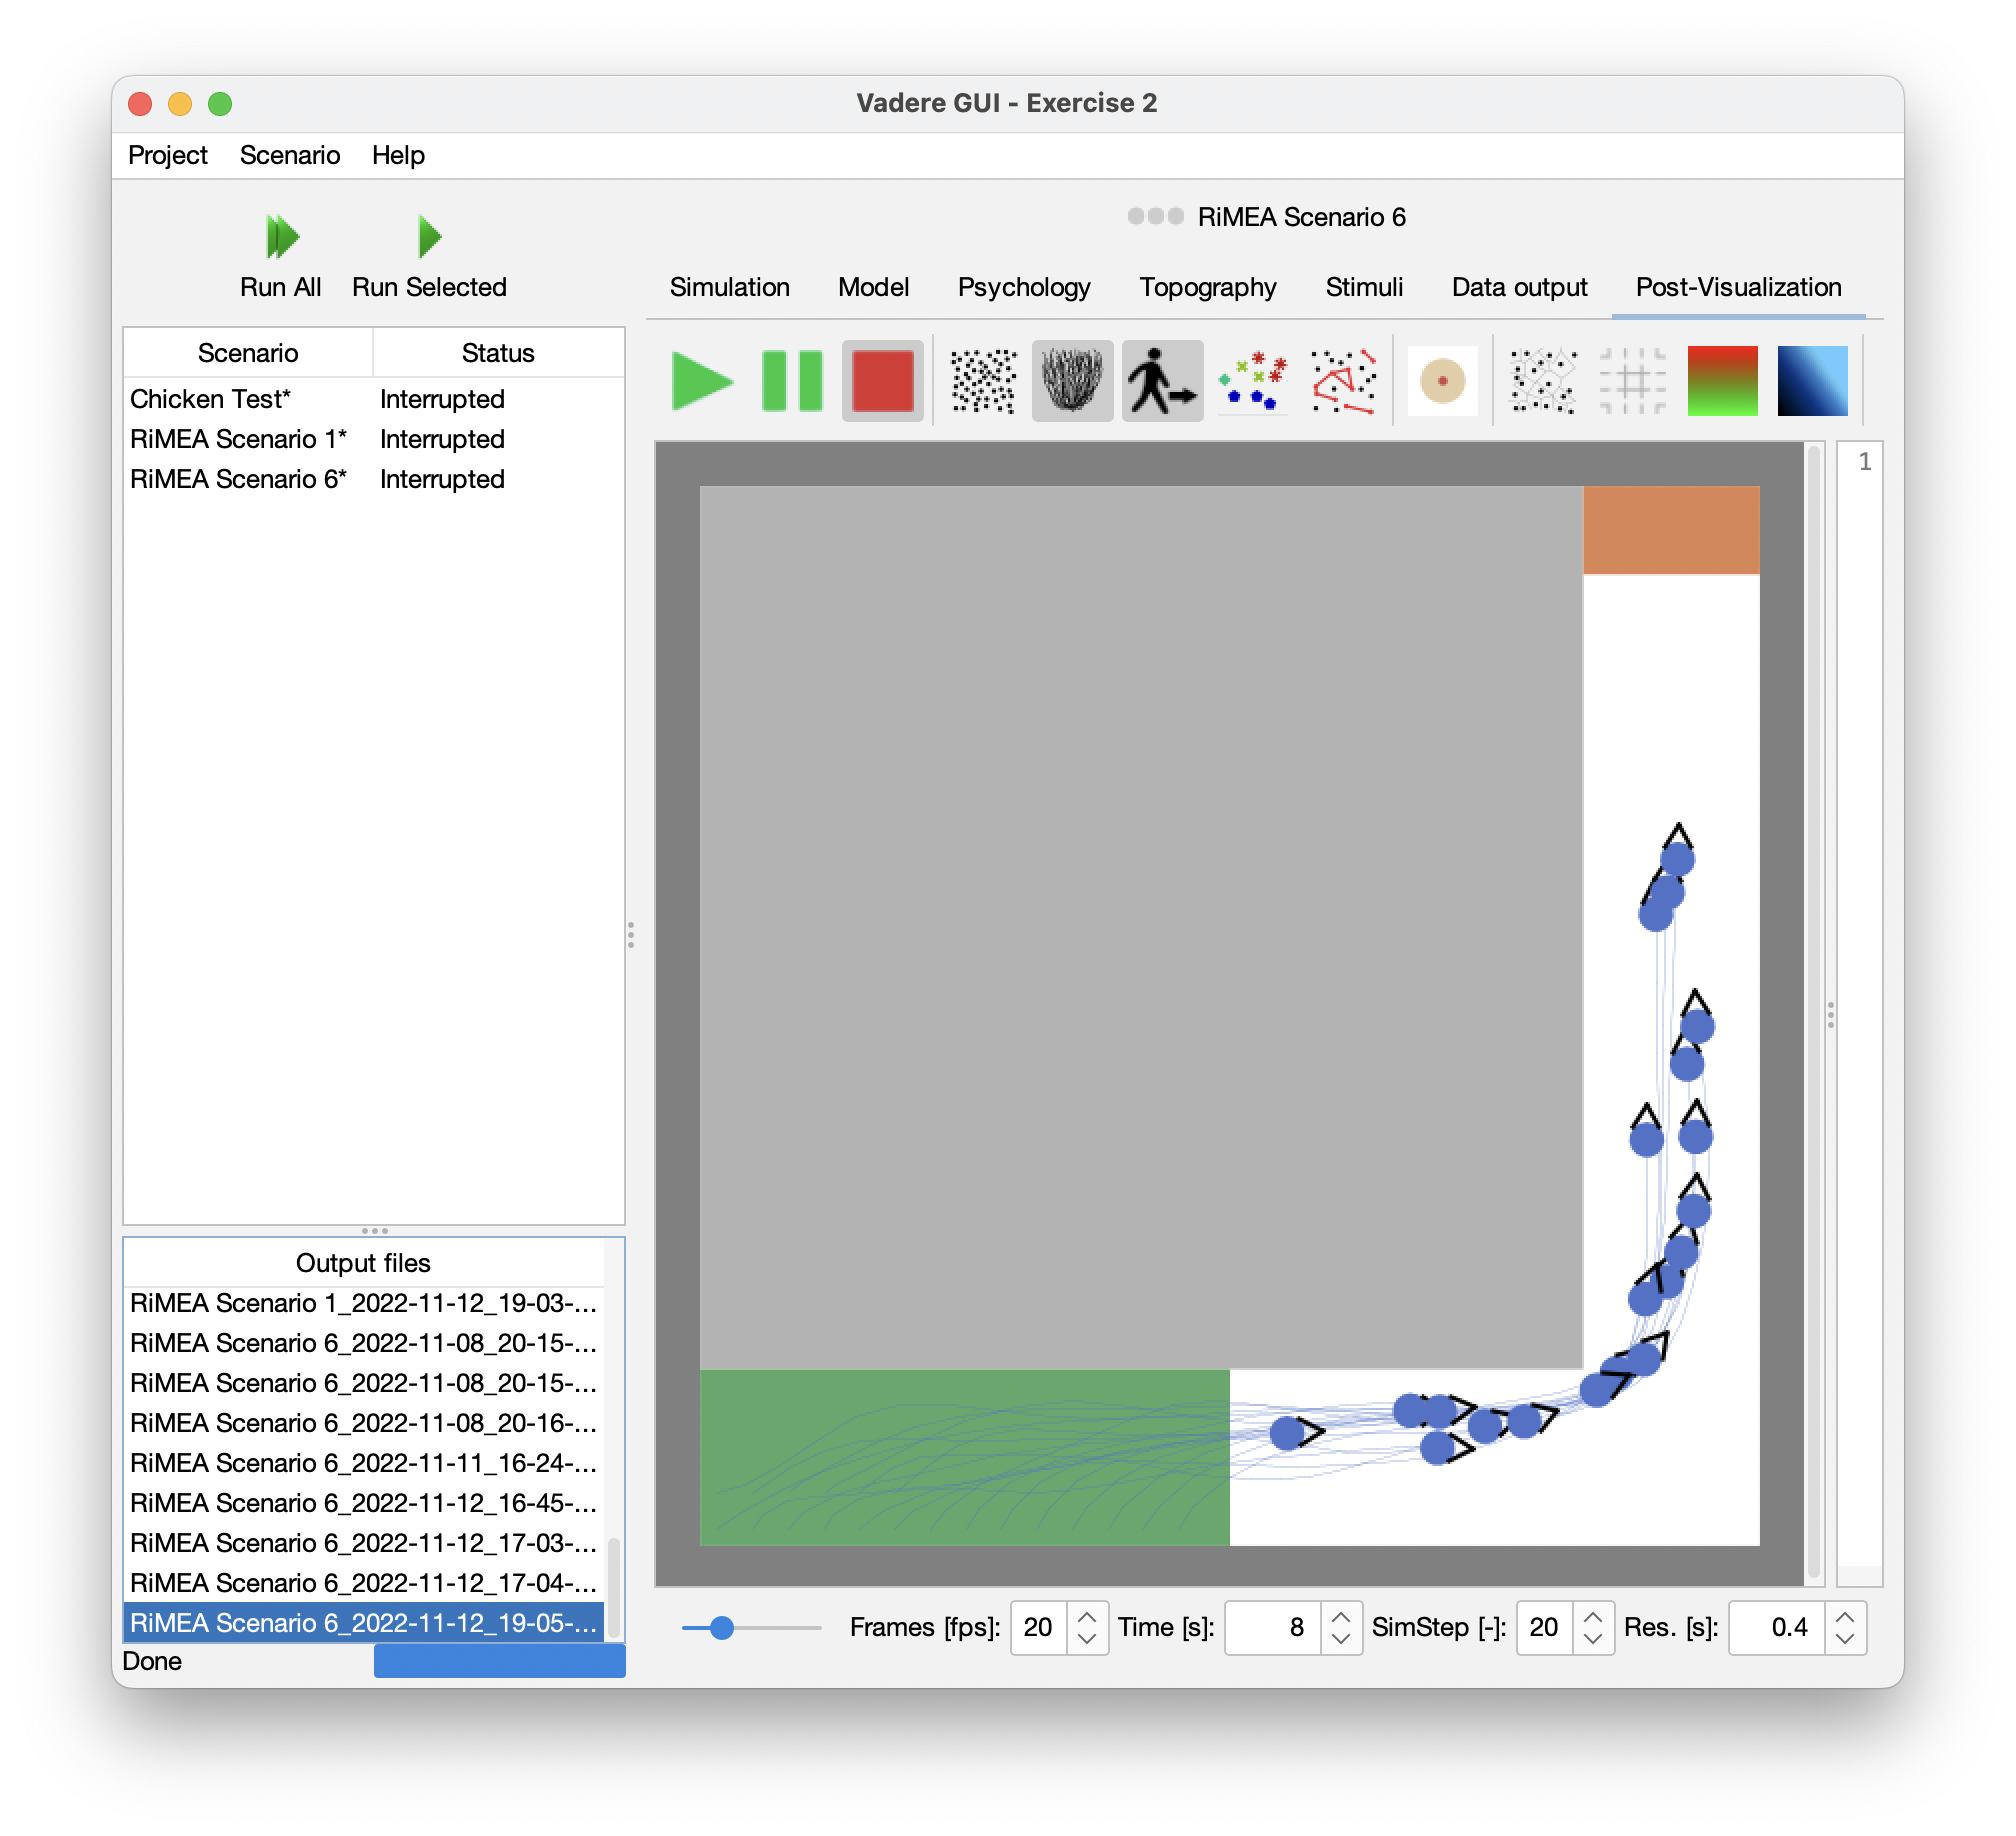
\includegraphics[width=0.33\textwidth]{images/sfm_6b.png}}
        \subfloat[At the end of the simulation]{
        \label{sfm_6c}
        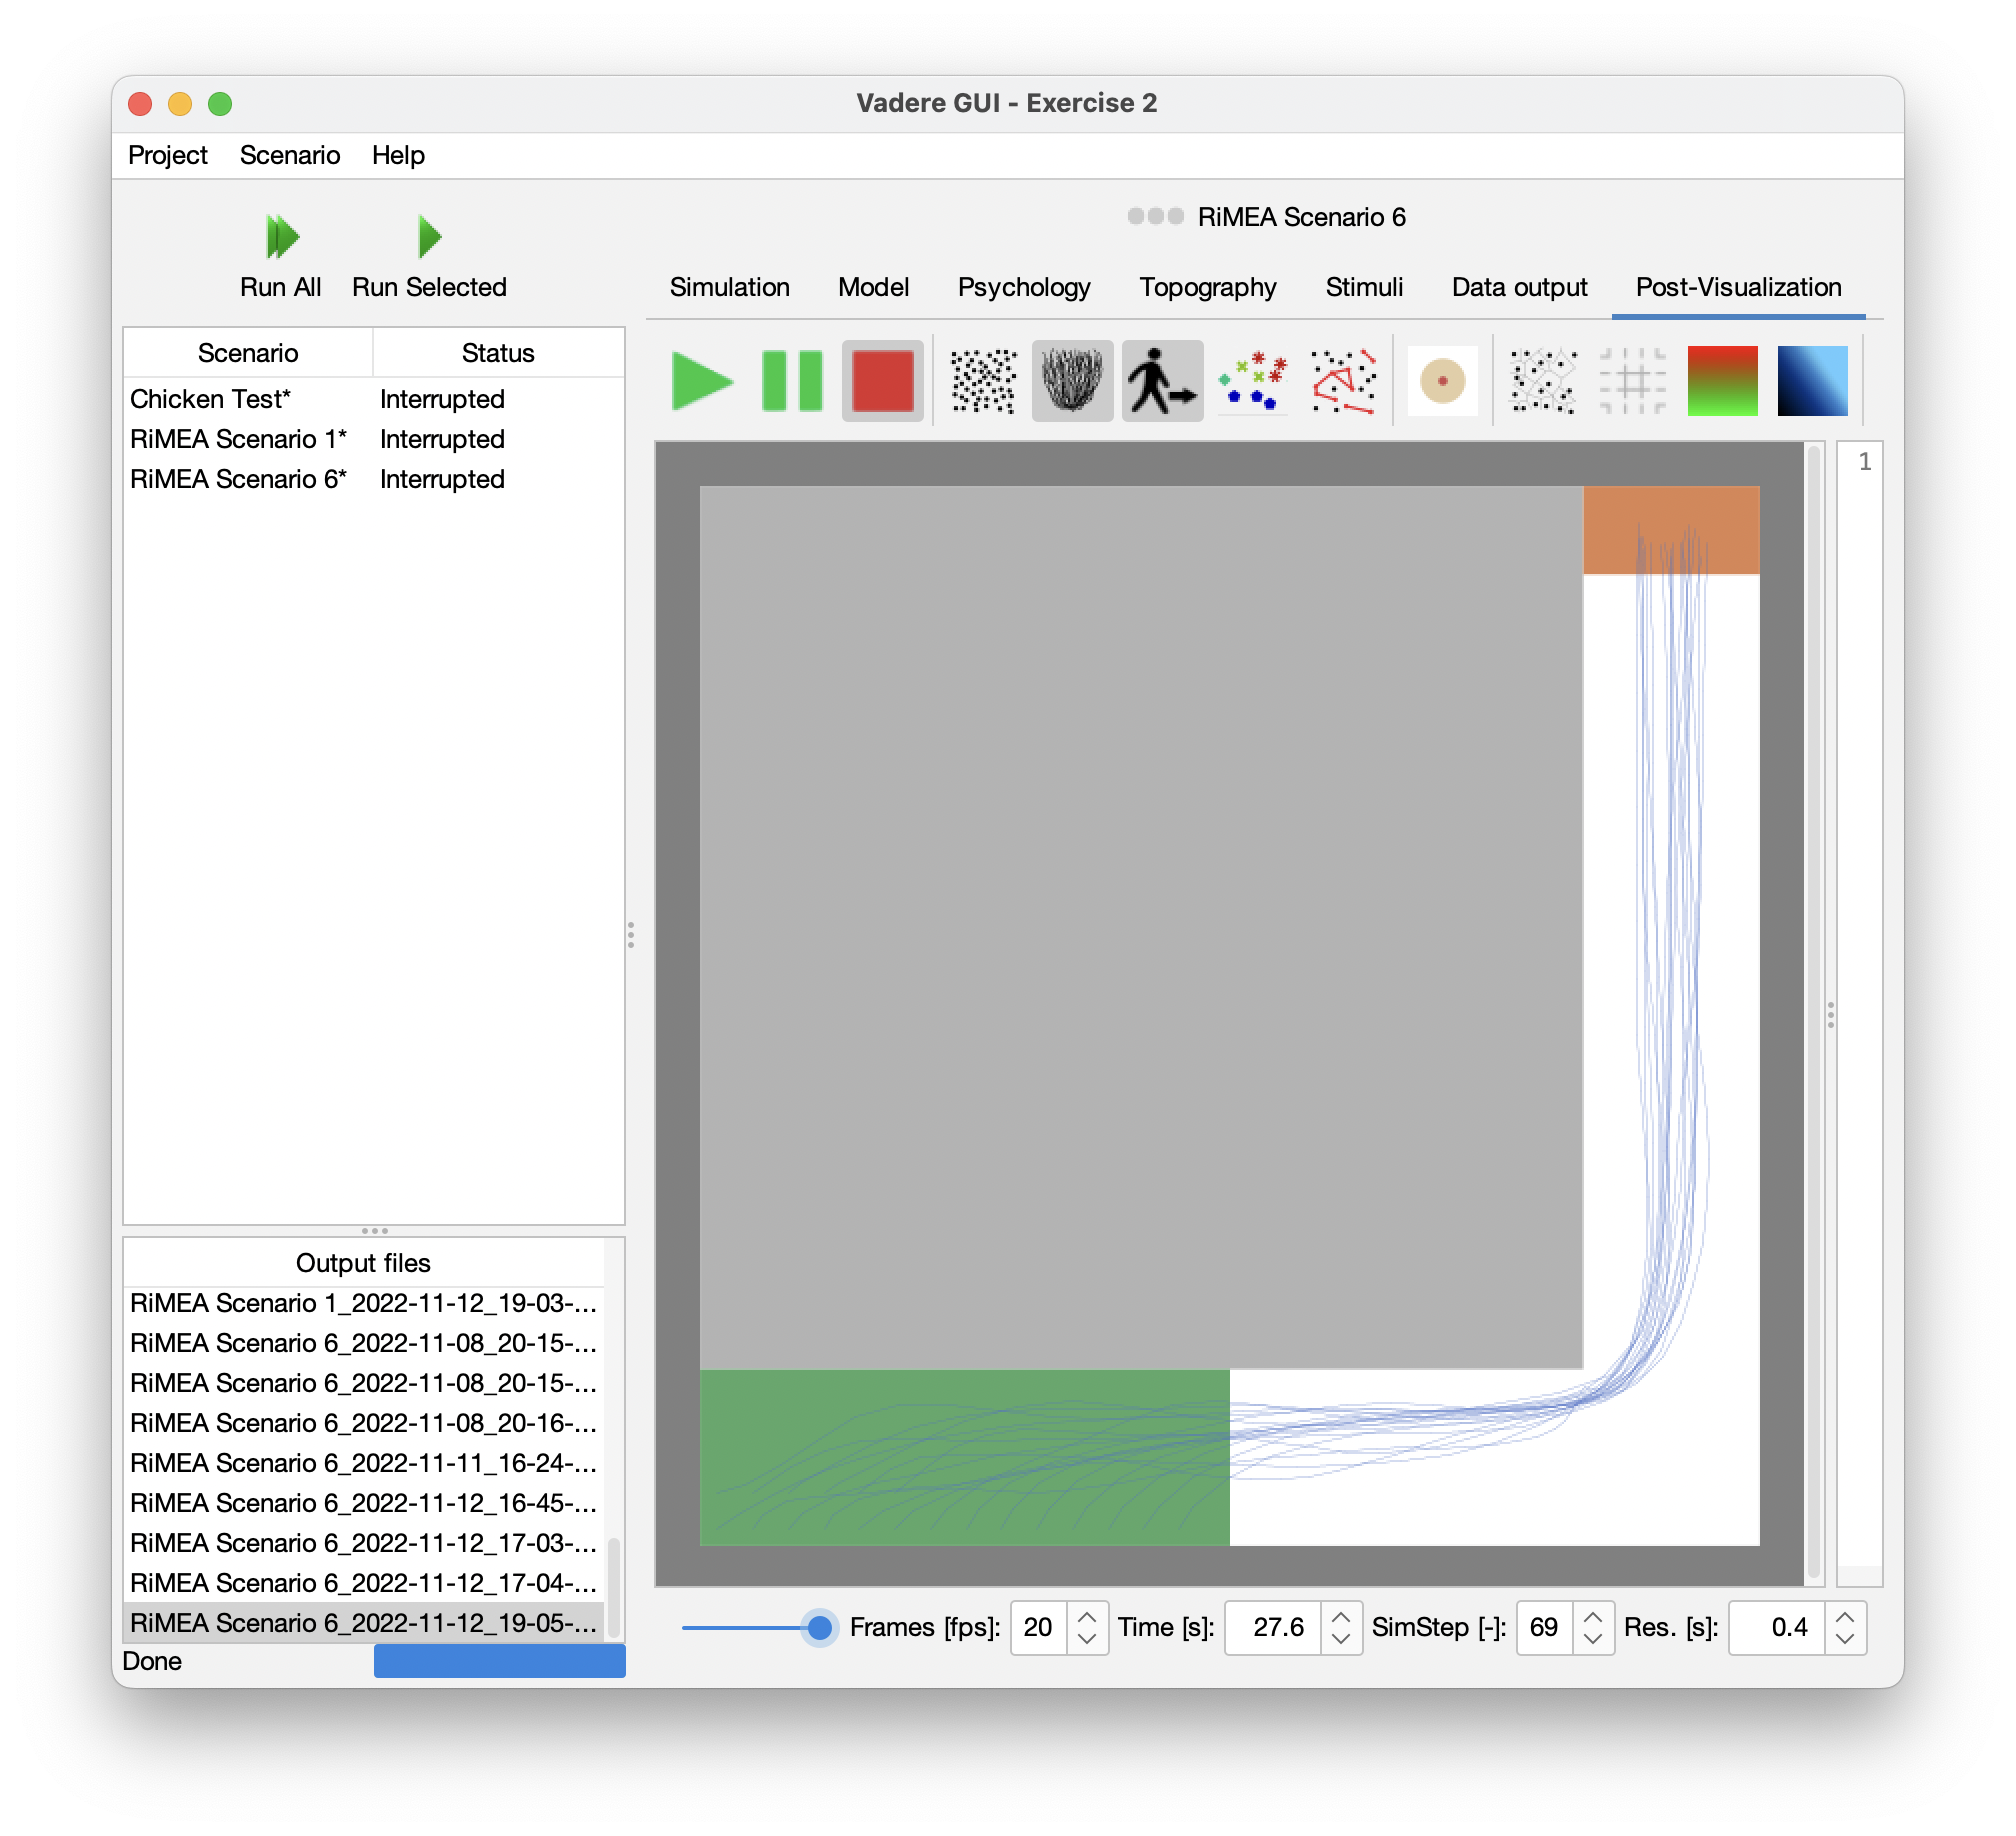
\includegraphics[width=0.33\textwidth]{images/sfm_6c.png}}
        \caption{Different stages of the simulation of the scenario 1 using the Gradient Navigation Model}
        \label{scenario6_sfm}
    \end{figure}
    
    \item Chicken test: of course, with the Social Force Model, the pedestrians can also avoid the obstacles and reach the target. As said in the previous case, the behavior of the pedestrians are more direct, ordered and natural in SFM than in OSM. It seems like the pedestrians know from the beginning where they have to go to reach the target, whereas in OSM although all of the pedestrians can avoid the obstacles and reach the target, some of them during the path collide with each other and obstacles and their paths are not as smoothly as the paths of the SFM (Figure \ref{sfm_chicken}, there are some big changes of directions from a pedestrian. The consequences also are reflected in the travel time with SFM - 32.4 s and with OSM - 34.57 s.
    
    \begin{figure} [H]
    \centering
    \subfloat[At the beginning of the simulation]{
        \label{sfm_chickena}
        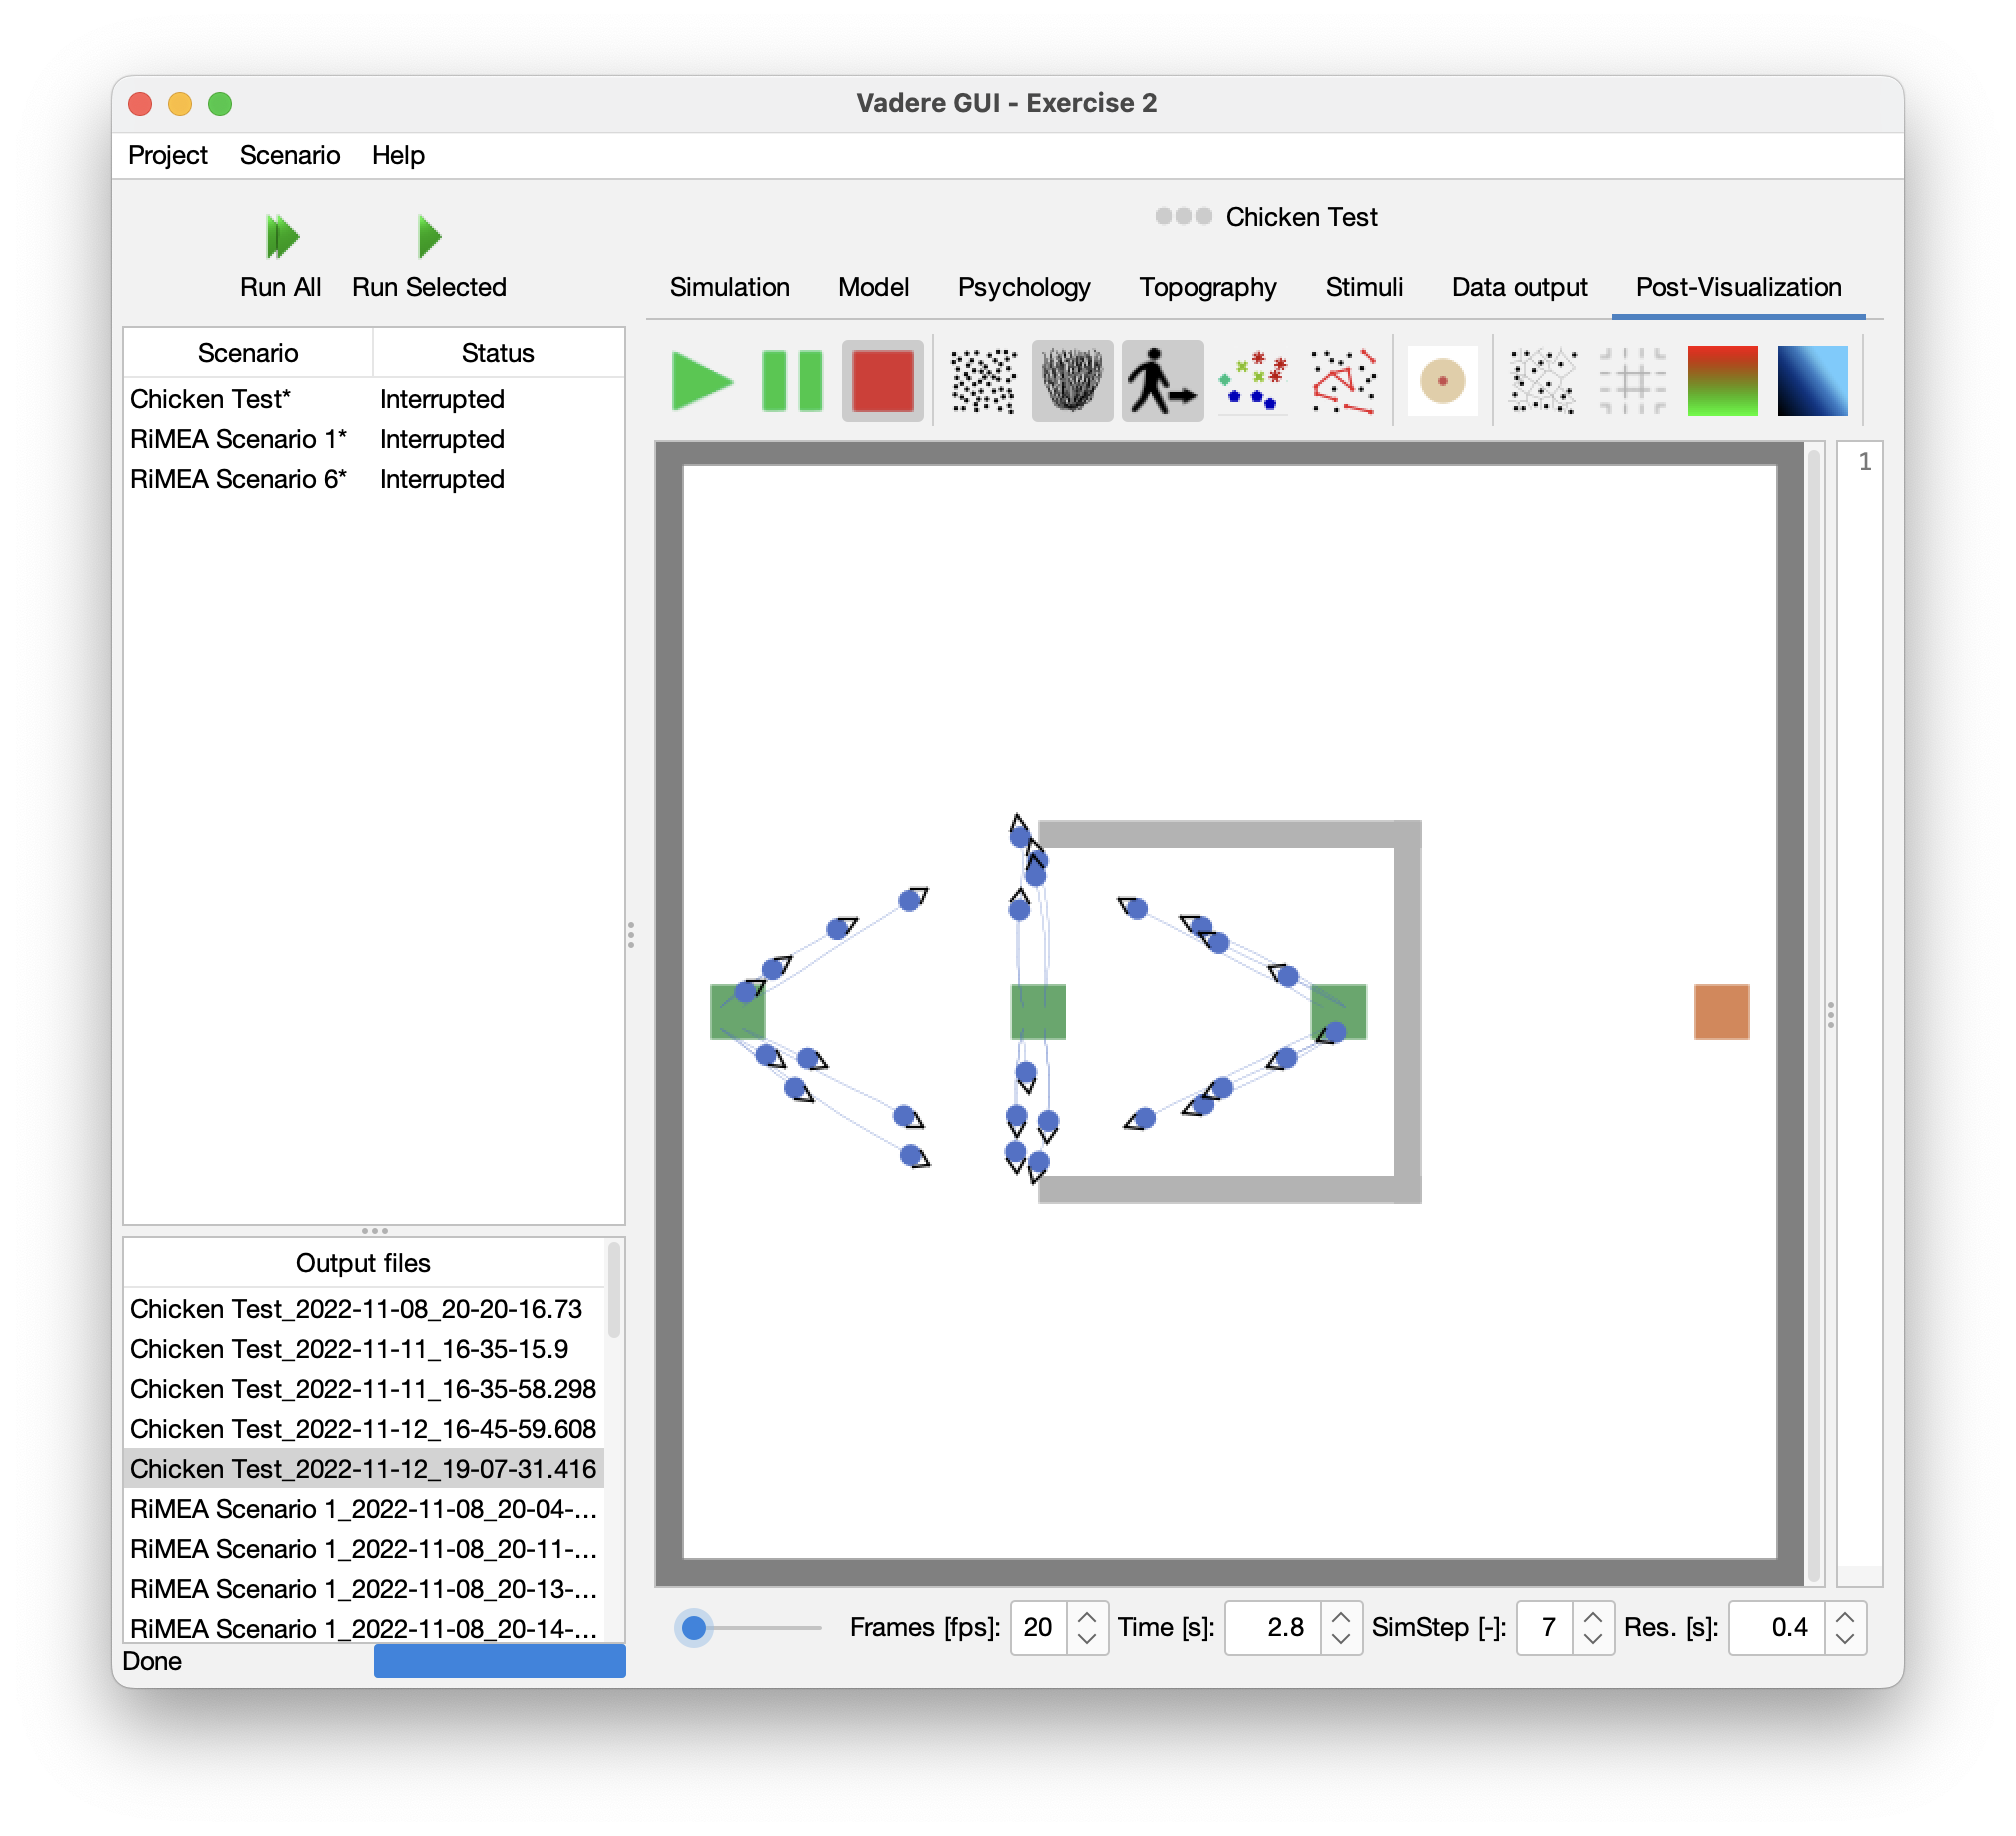
\includegraphics[width=0.33\textwidth]{images/sfm_chickena.png}}
        \subfloat[In the middle of the simulation]{
        \label{sfm_chickenb}
        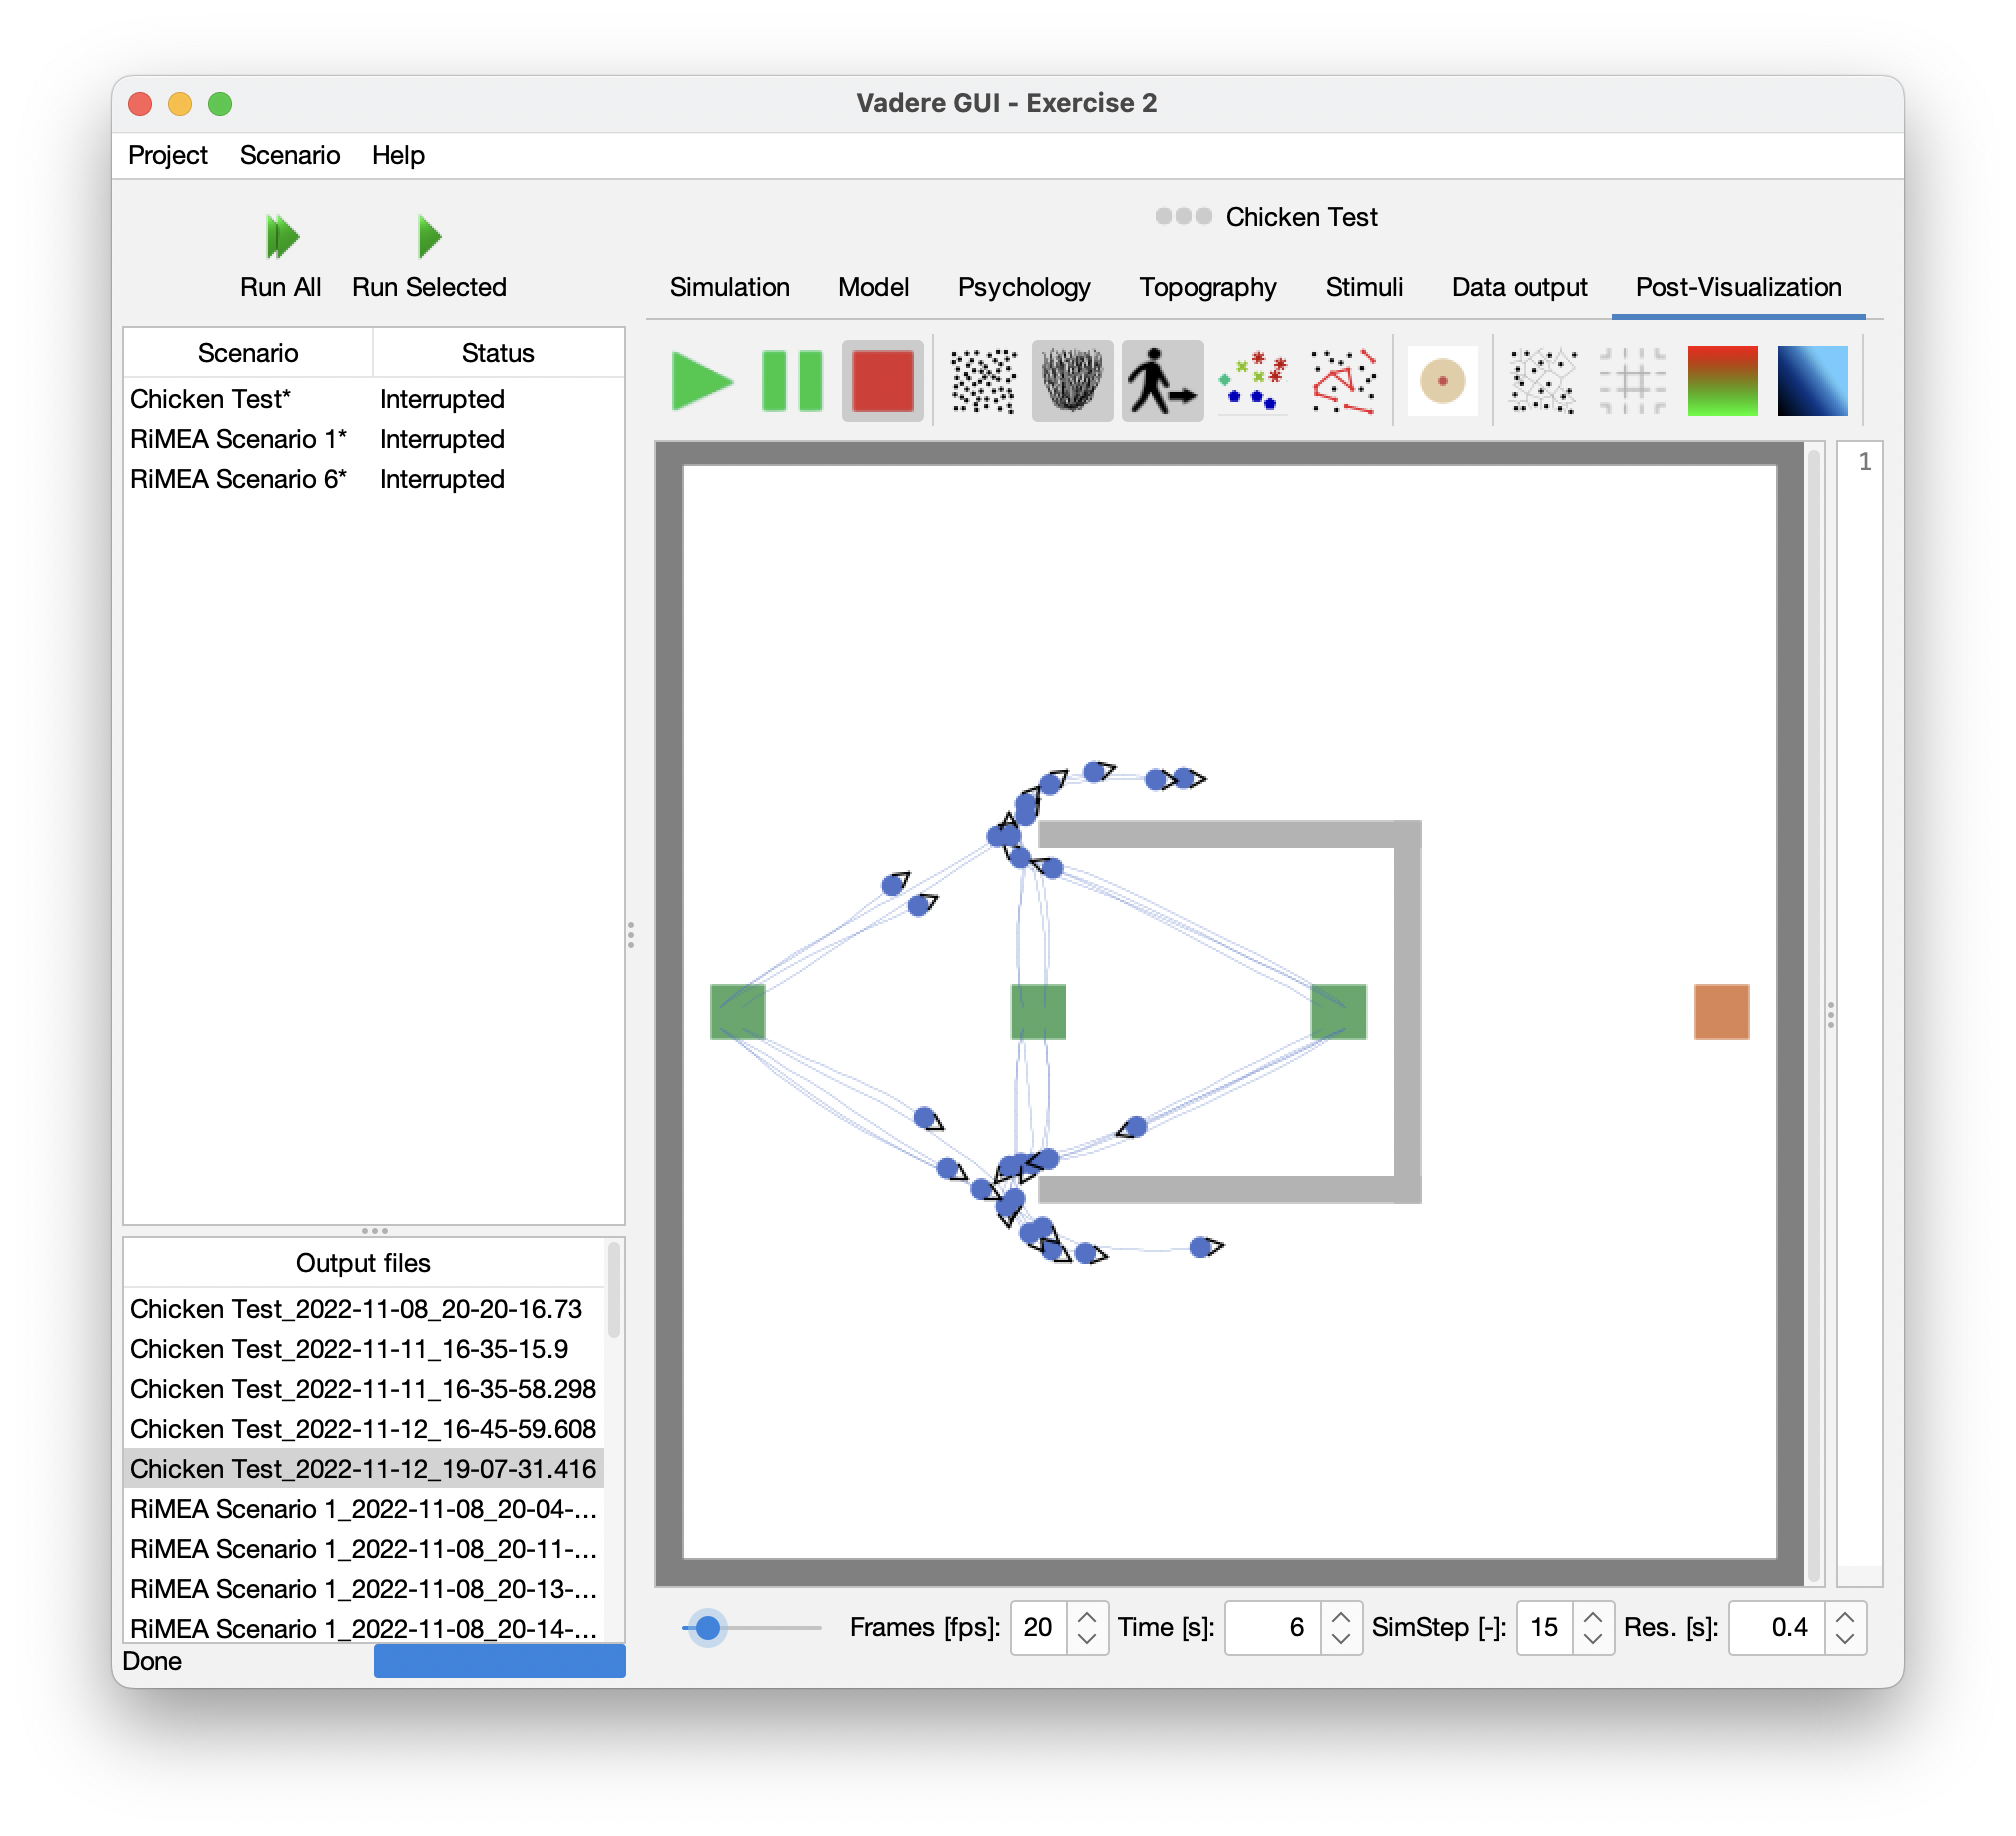
\includegraphics[width=0.33\textwidth]{images/sfm_chickenb.png}}
        \subfloat[At the end of the simulation]{
        \label{sfm_chickenc}
        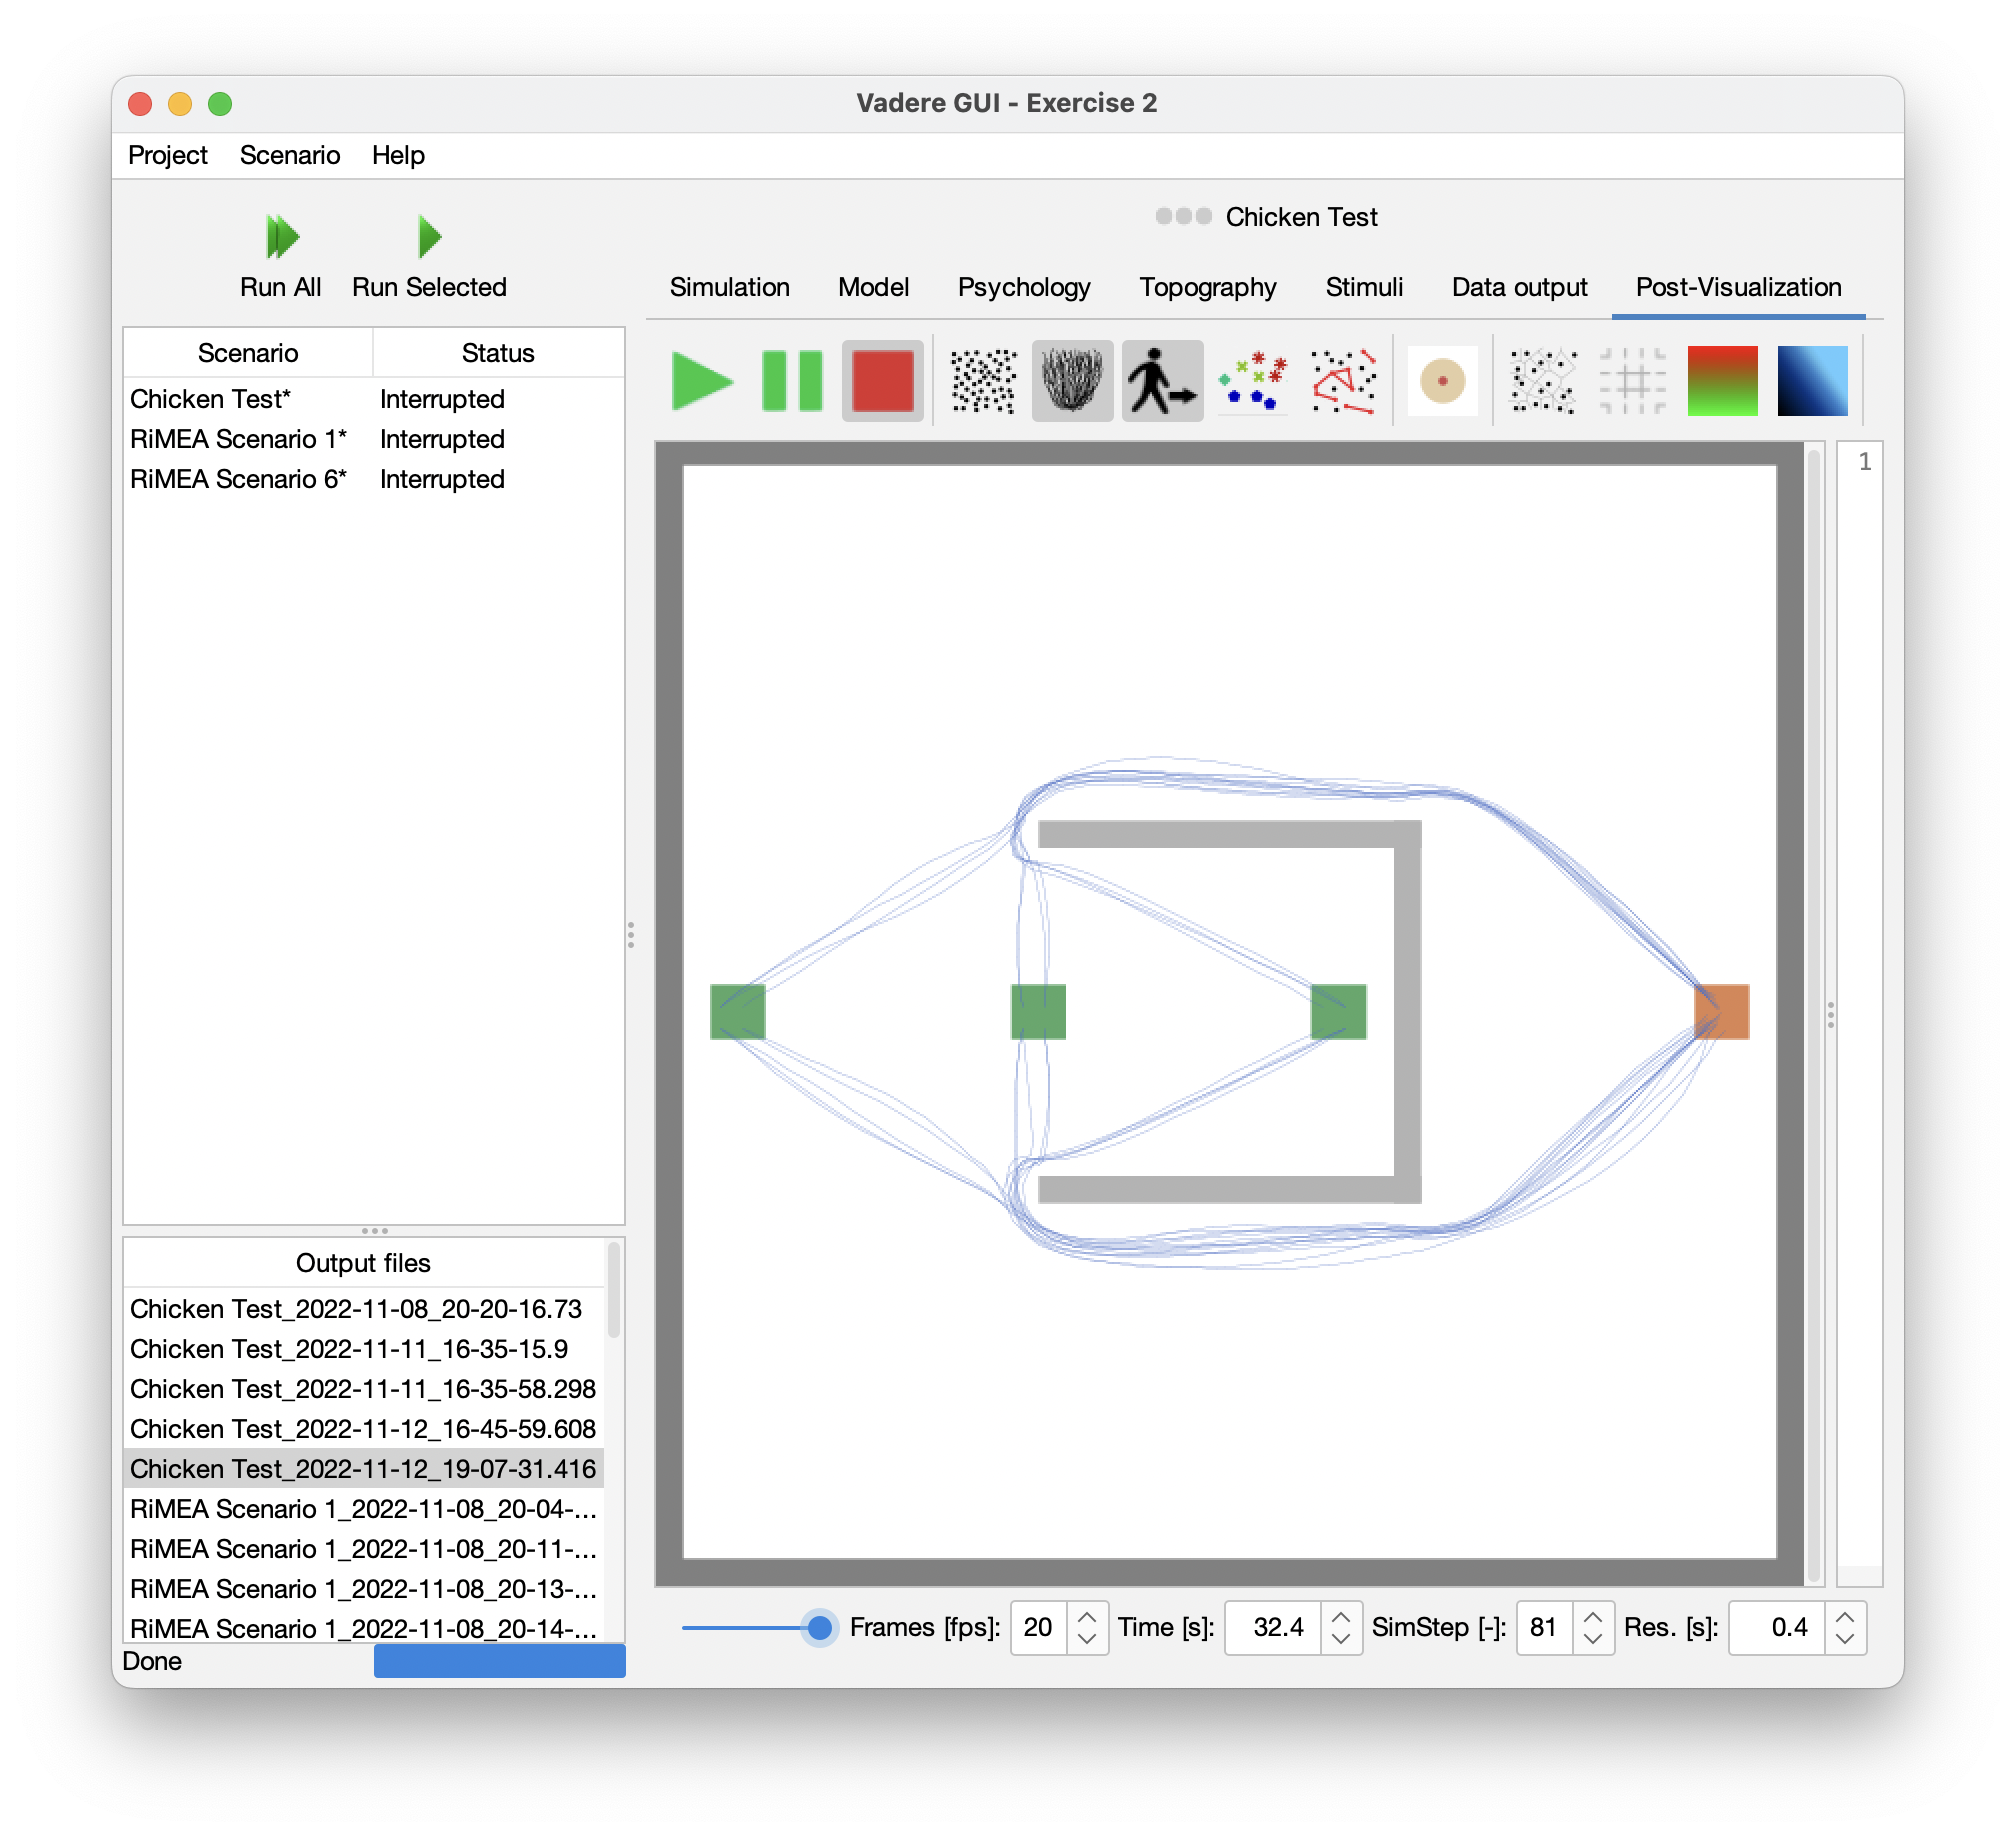
\includegraphics[width=0.33\textwidth]{images/sfm_chickenc.png}}
        \caption{Different stages of the simulation of the chicken test using the Social Force Model}
        \label{chicken_sfm}
    \end{figure}
    
\end{enumerate}

\bigskip

\noindent{\textbf{Gradient Navigation Model (GNM)}}

\begin{enumerate}[label=(\alph*)]
    \item RiMEA scenario 1: the pedestrian does not follow a straight line anymore, instead, it moves downwards until the target is reached. The travel time in both simulations are roughly the same, being the simulation using GNM slightly faster, but negligible. This new behaviour is due most probably to how a target surface works: by looking at the results using OSM (Figure \ref{scenario1_sim}), it can be observed that the pedestrian turns up right before reaching the target, instead of keeping a completely straight path, so it is possible that the target itself can be reached through different points inside it. By taking this into account, for this case the pedestrian might have selected a lower point in the target, and therefore there might have been some anticipation while selecting the path. However, since not much information is given, this conclusion cannot be ensured.
    
    \begin{figure} [H]
    \centering
    \subfloat[At the beginning of the simulation]{
        \label{gnm_1a}
        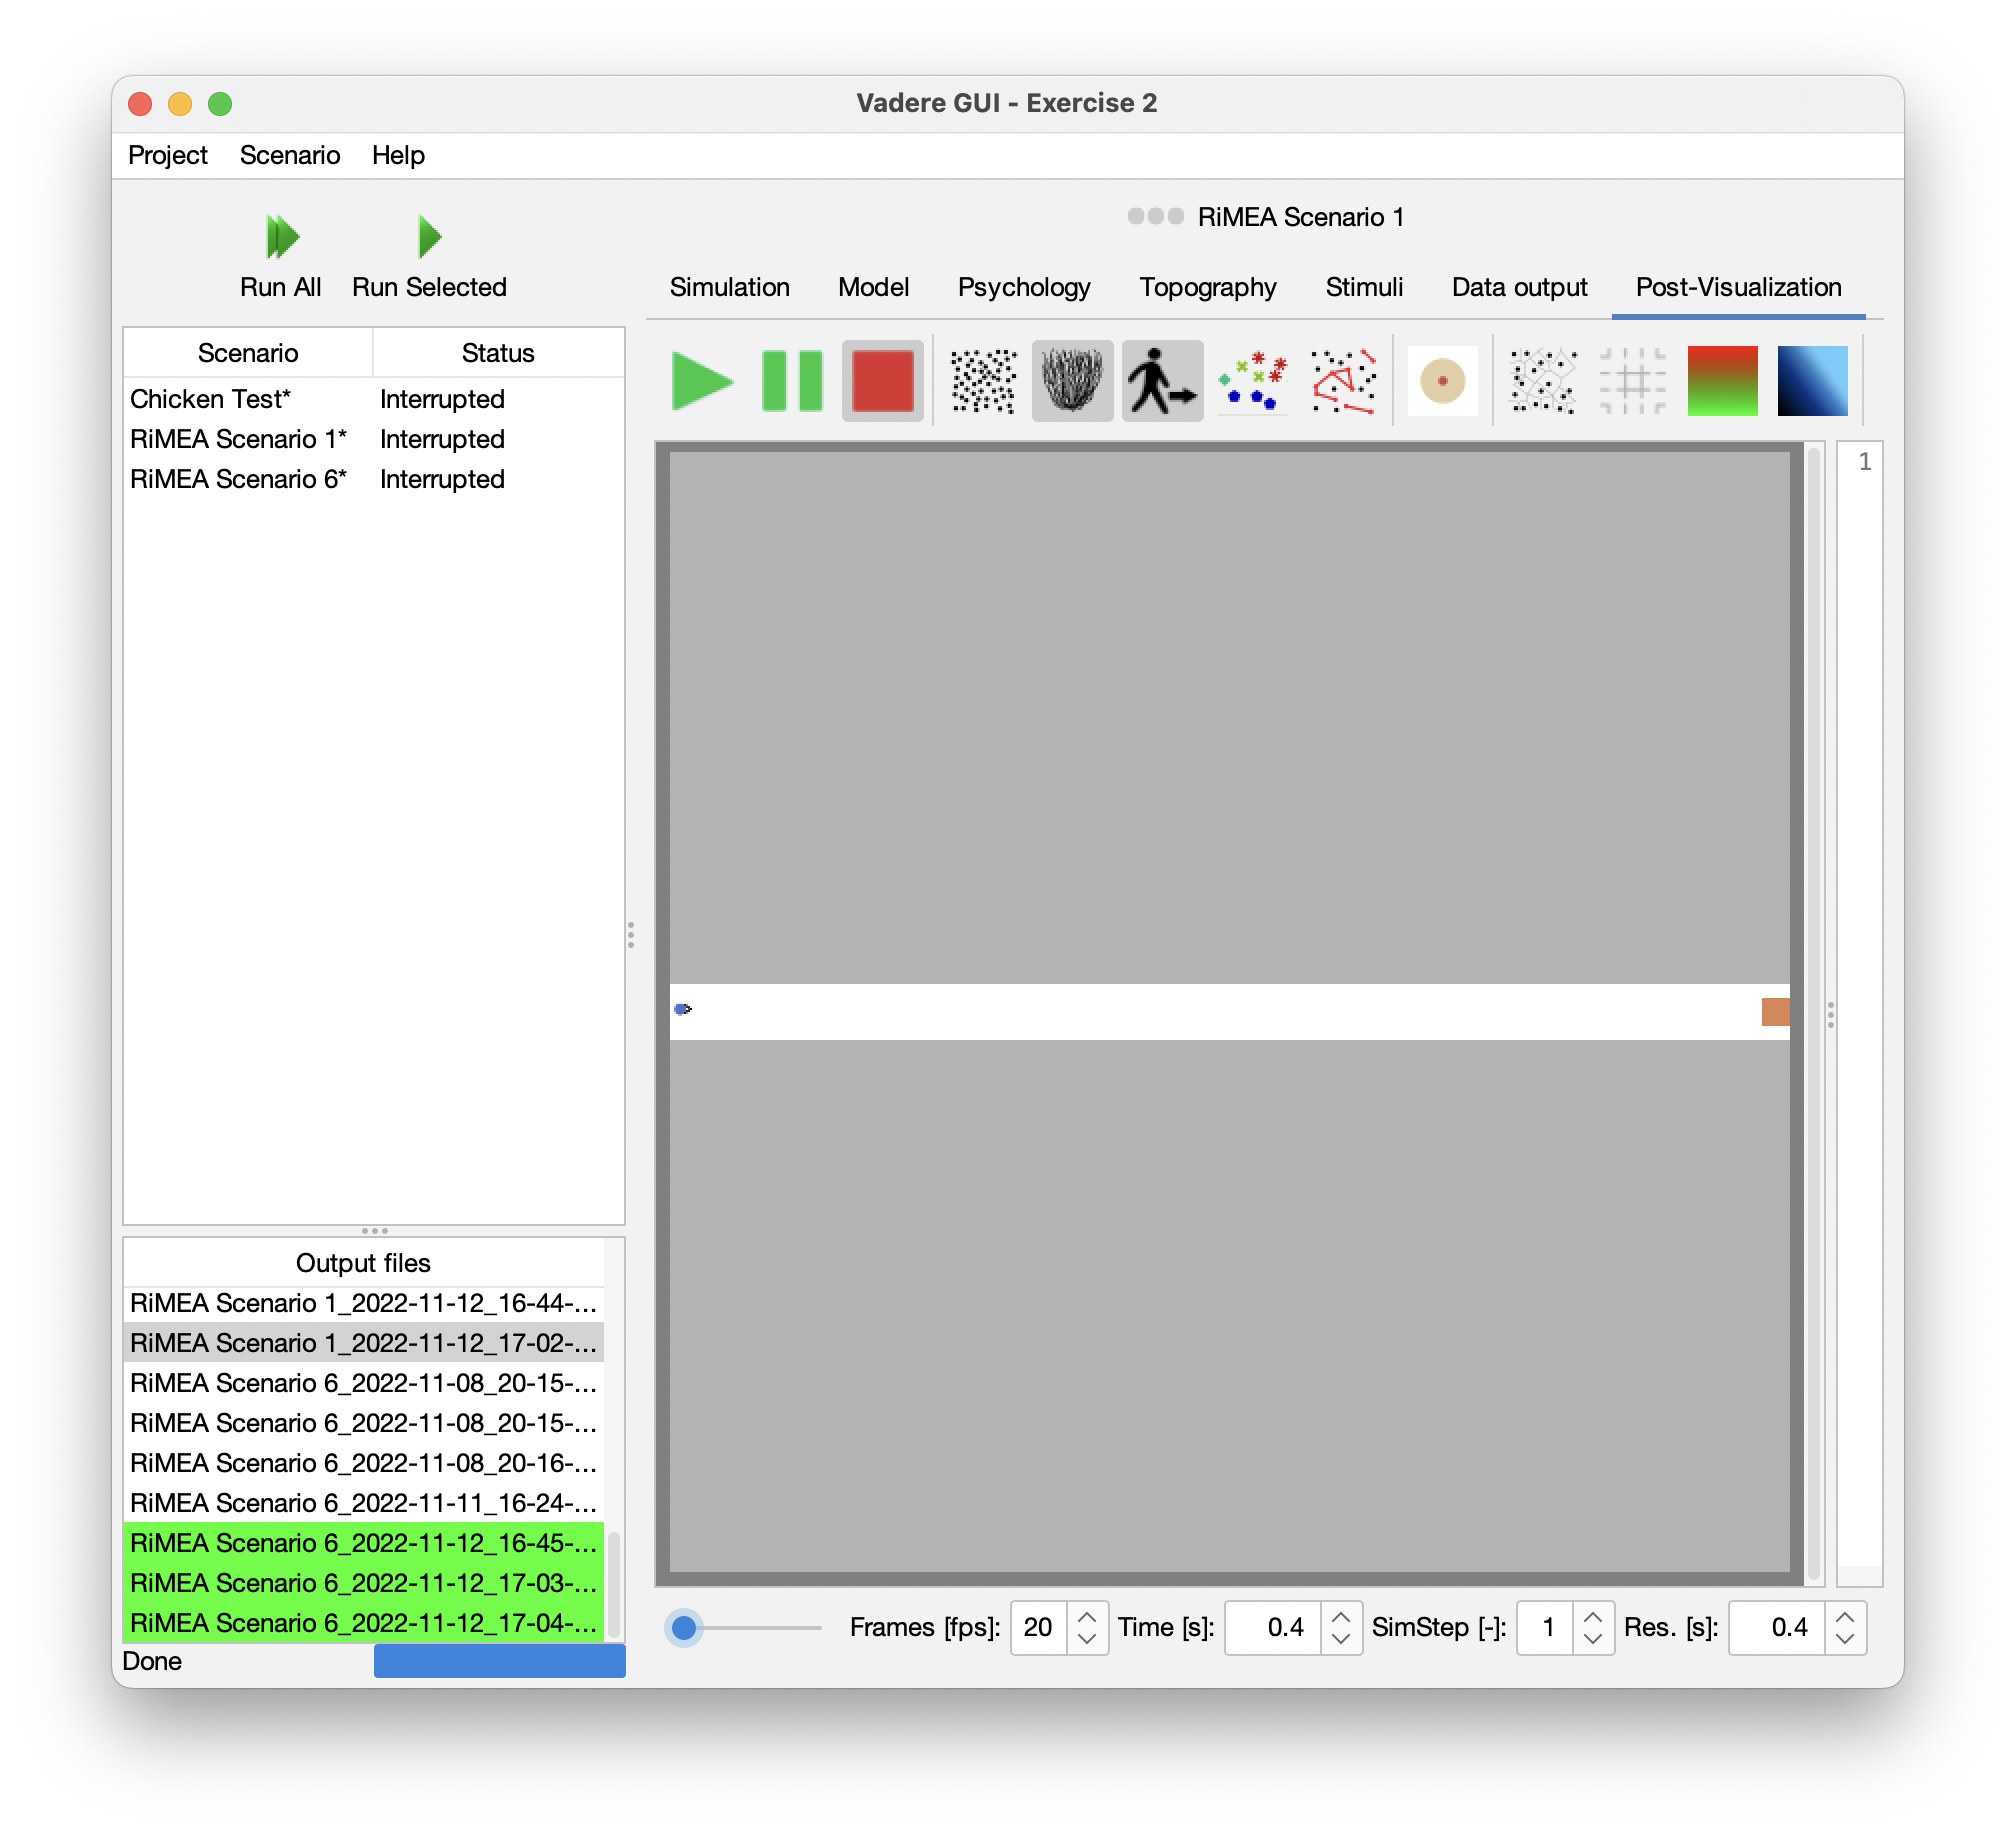
\includegraphics[width=0.33\textwidth]{images/gnm_1a.png}}
        \subfloat[In the middle of the simulation]{
        \label{gnm_1b}
        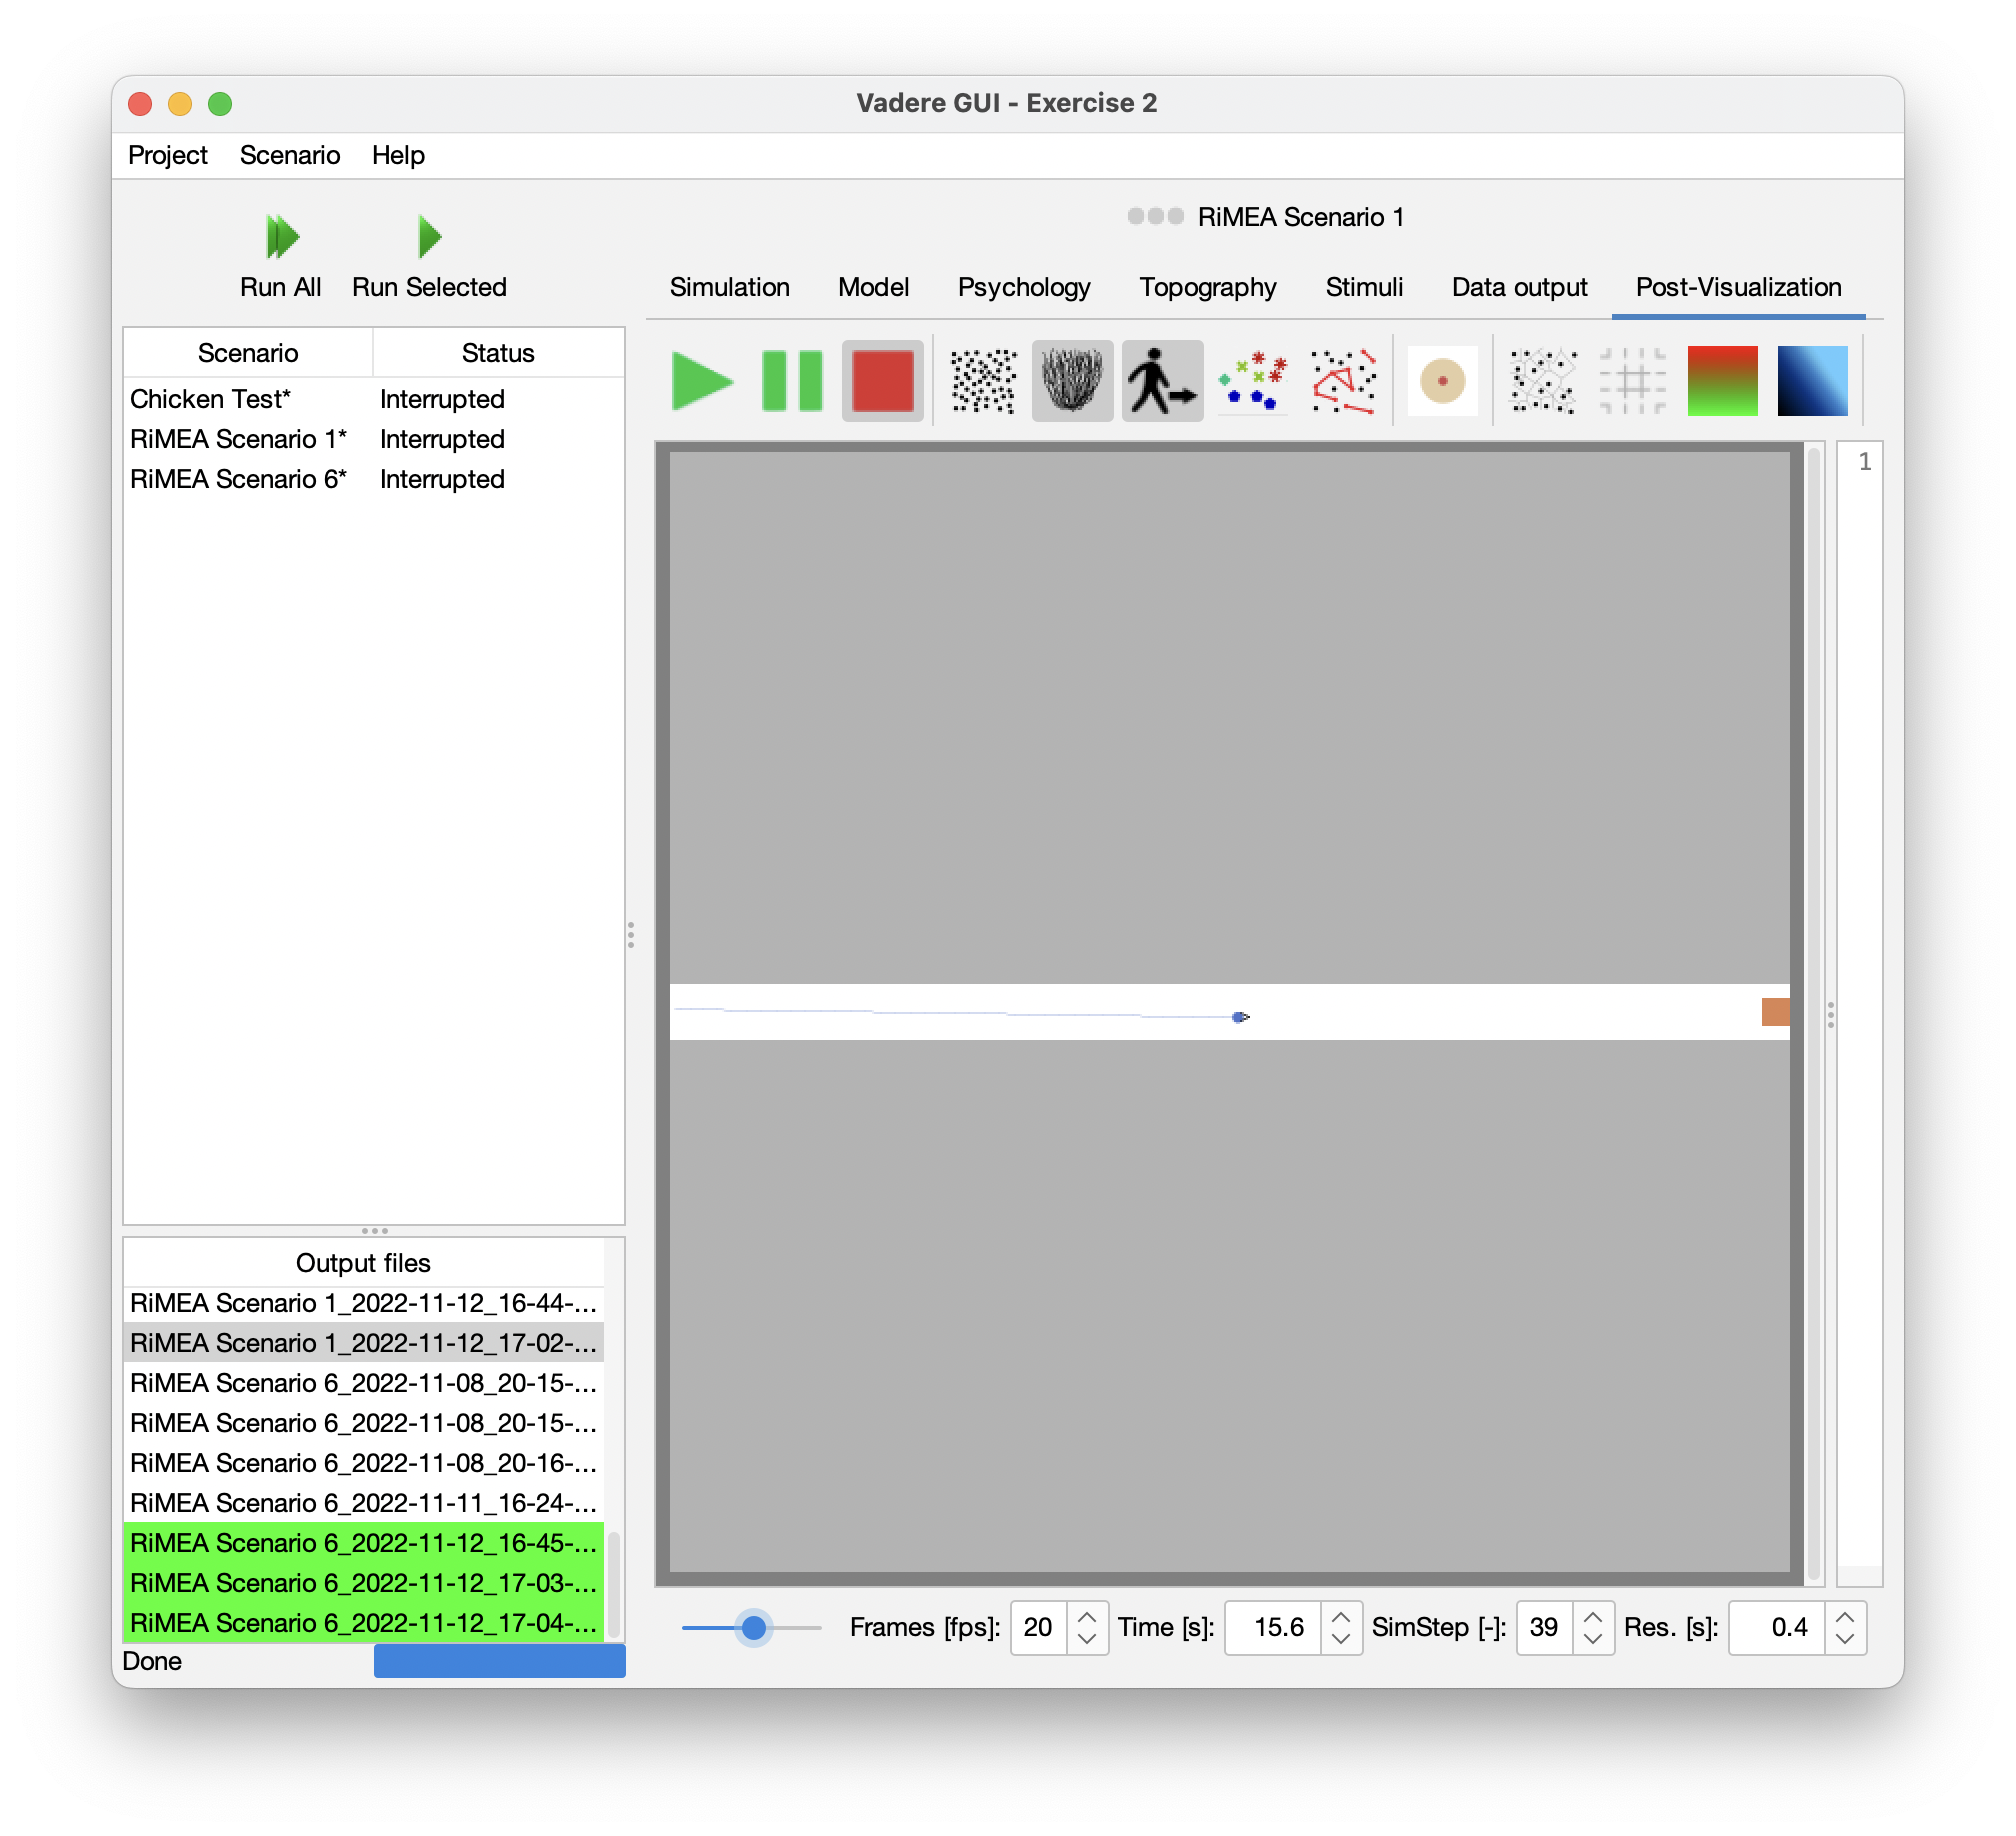
\includegraphics[width=0.33\textwidth]{images/gnm_1b.png}}
        \subfloat[At the end of the simulation]{
        \label{gnm_1c}
        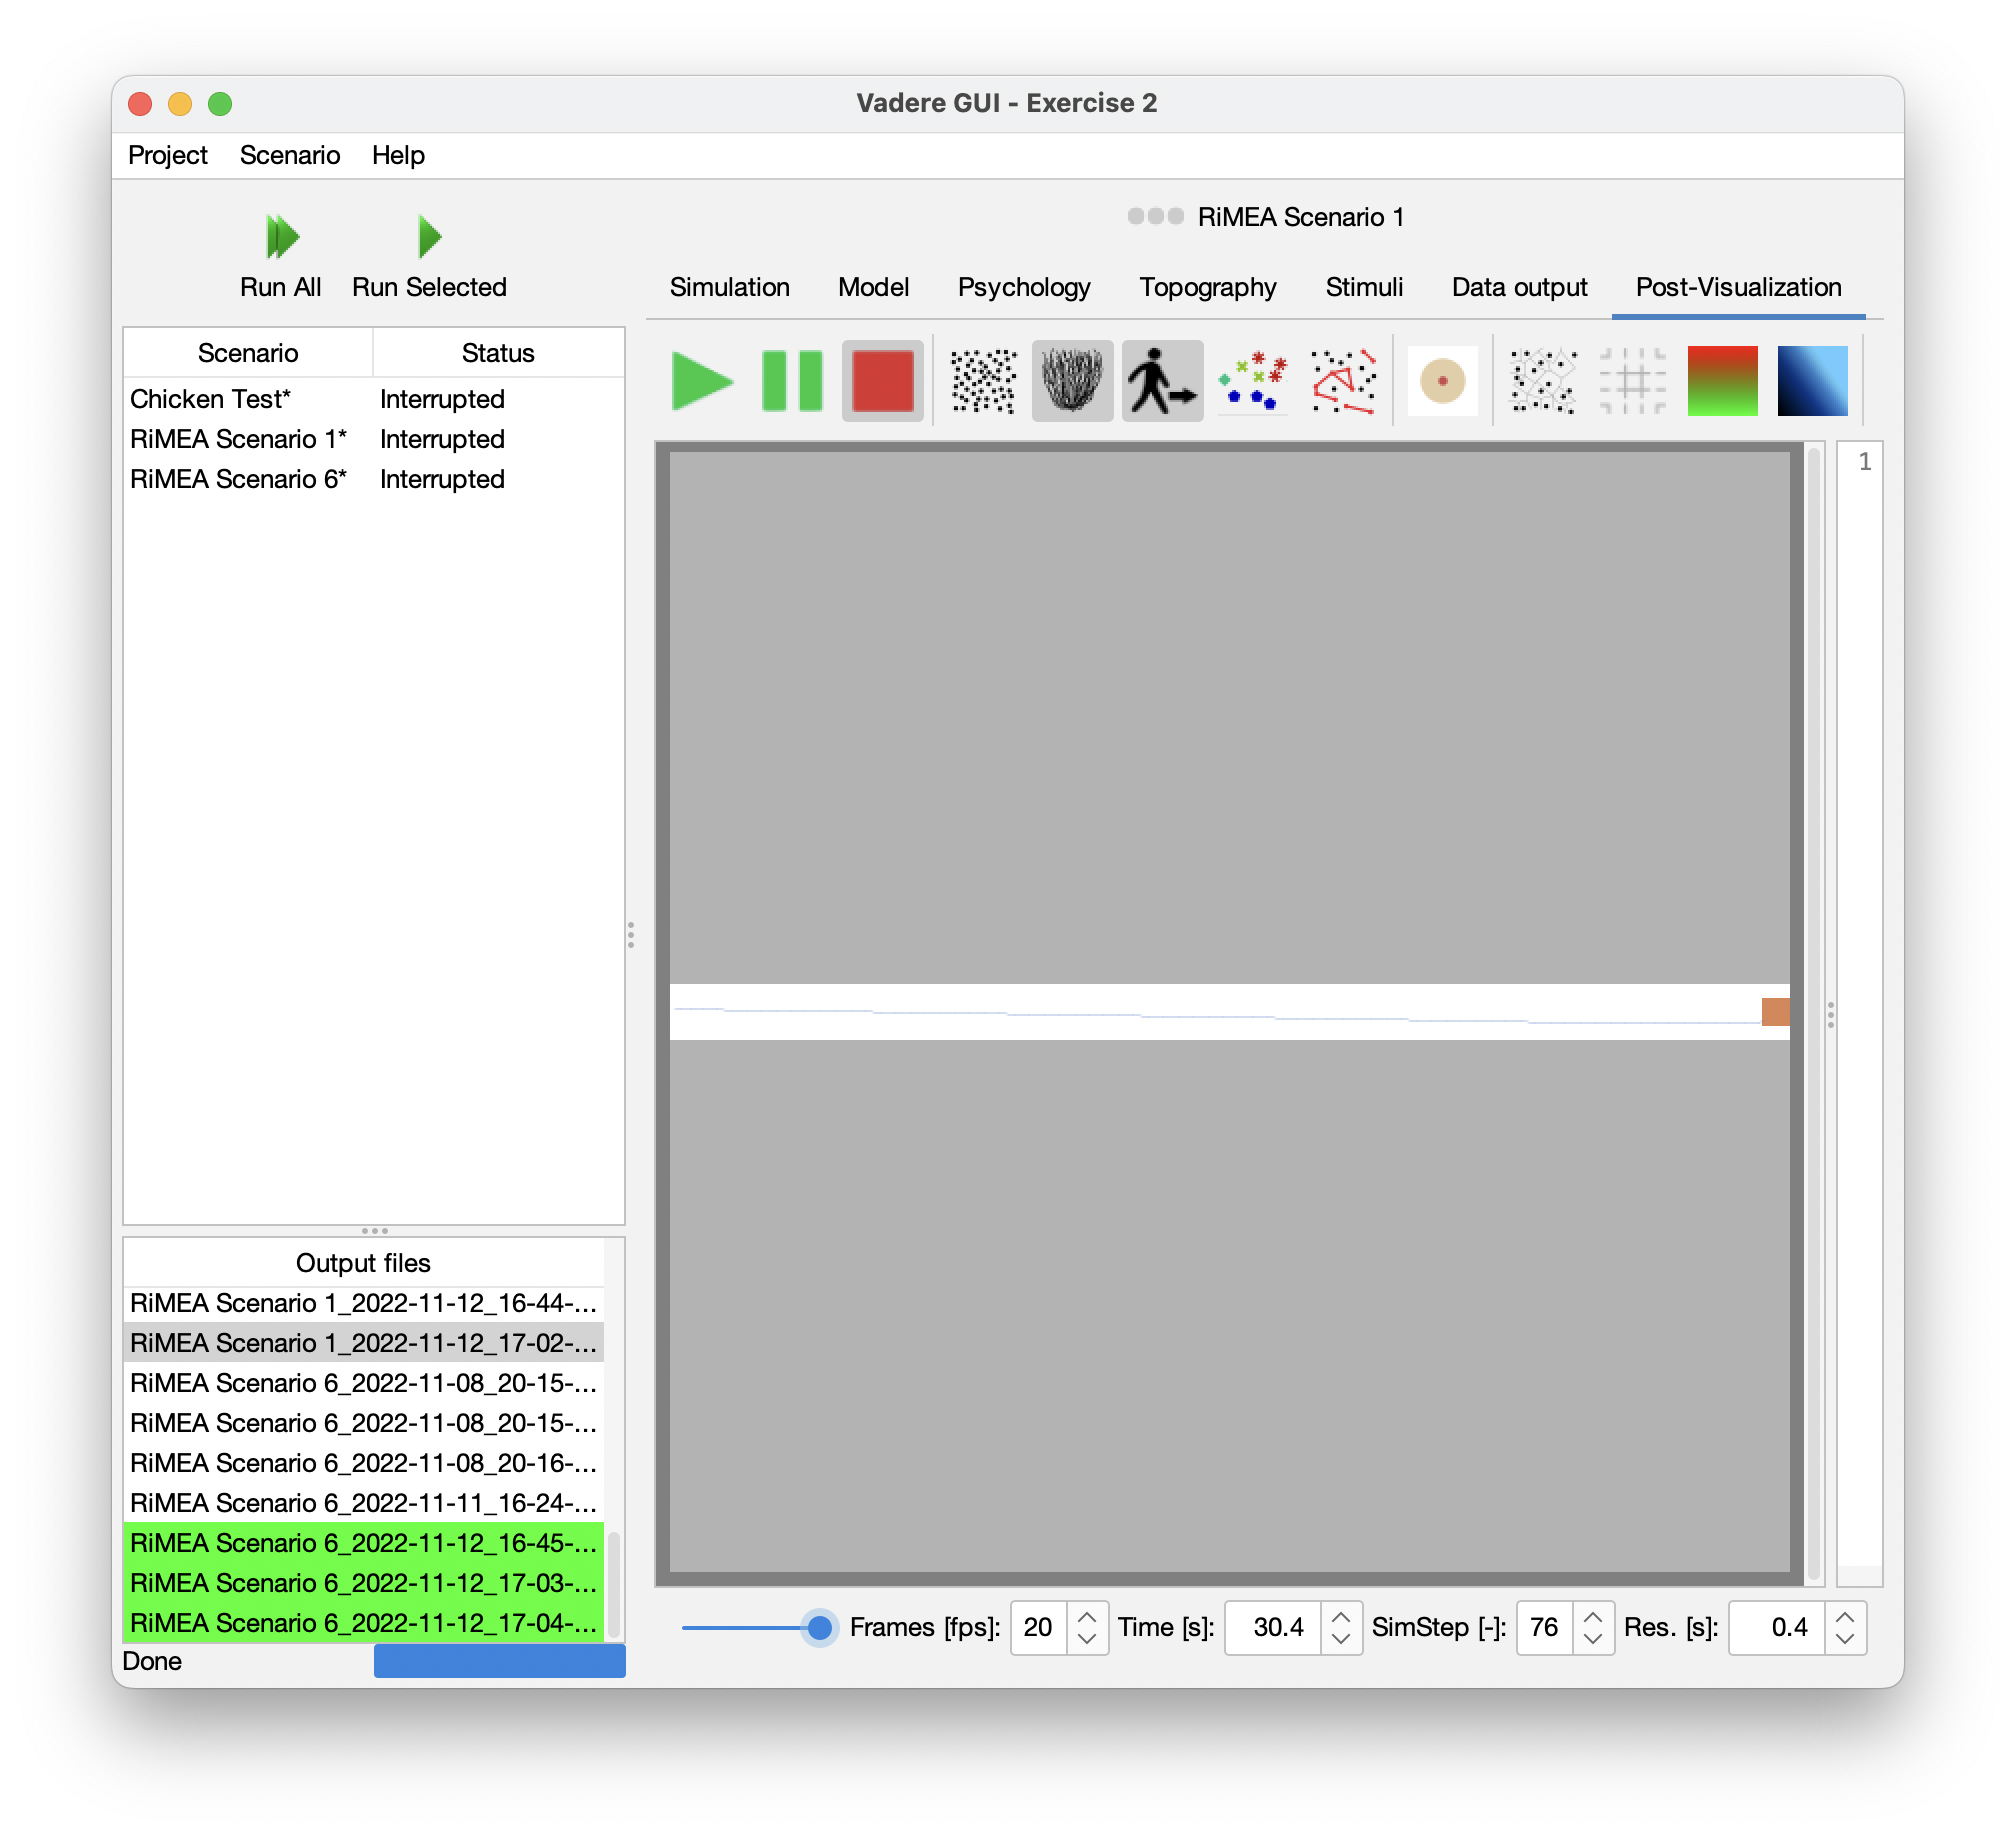
\includegraphics[width=0.33\textwidth]{images/gnm_1c.png}}
        \caption{Different stages of the simulation of the scenario 1 using the Gradient Navigation Model}
        \label{scenario1_gnm}
    \end{figure}
    
    \item RiMEA scenario 6: for this scenario, except for two pedestrians, all of them ended up doing the same uniform path as the one who reached the target first, without passing through walls. All pedestrians seemed to be more organised, as if they already knew the path they should follow beforehand. Furthermore, whenever a pedestrian had any other pedestrian obstructing their path, their behaviour consisted in reducing their speeds and waiting until they were able to continue (with exceptions, as commented before), rather than taking another path, as the pedestrians in the simulation using OSM did (Figure \ref{scenario6_sim}). Due to this behaviour, the travel time increased about 8 seconds.
    
    \begin{figure} [H]
    \centering
    \subfloat[At the beginning of the simulation]{
        \label{gnm_6a}
        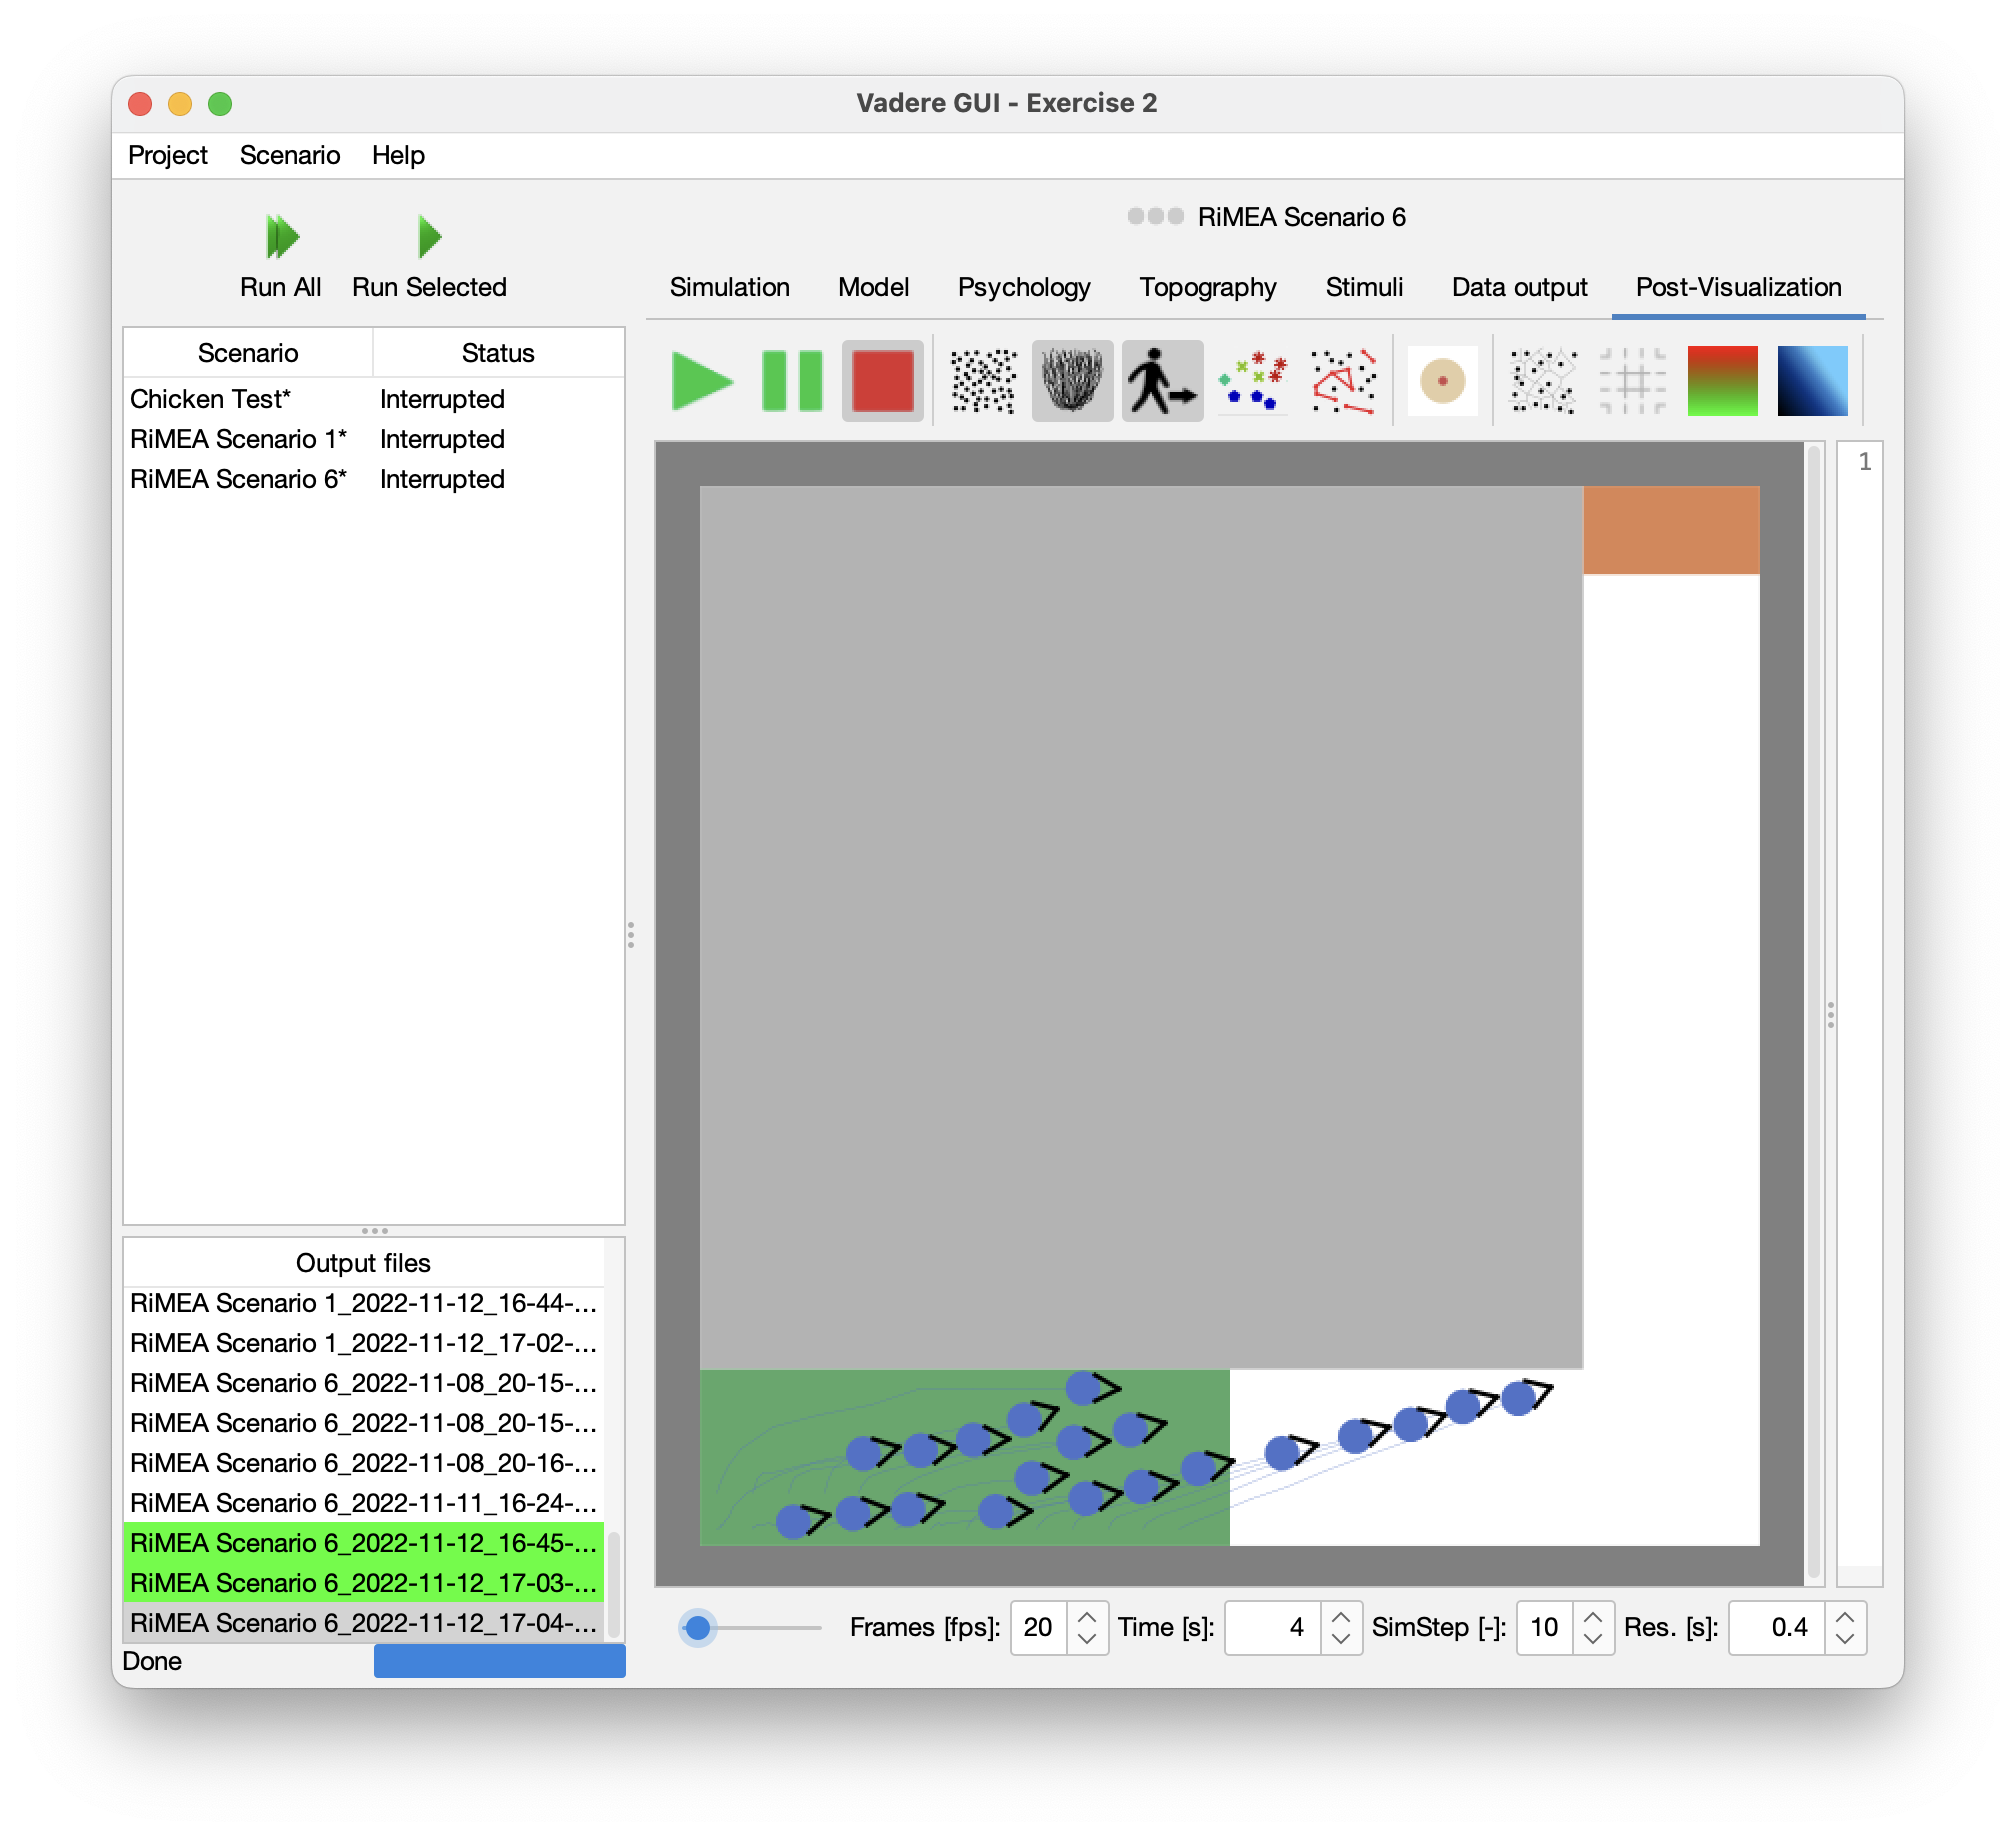
\includegraphics[width=0.33\textwidth]{images/gnm_6a.png}}
        \subfloat[In the middle of the simulation]{
        \label{gnm_6b}
        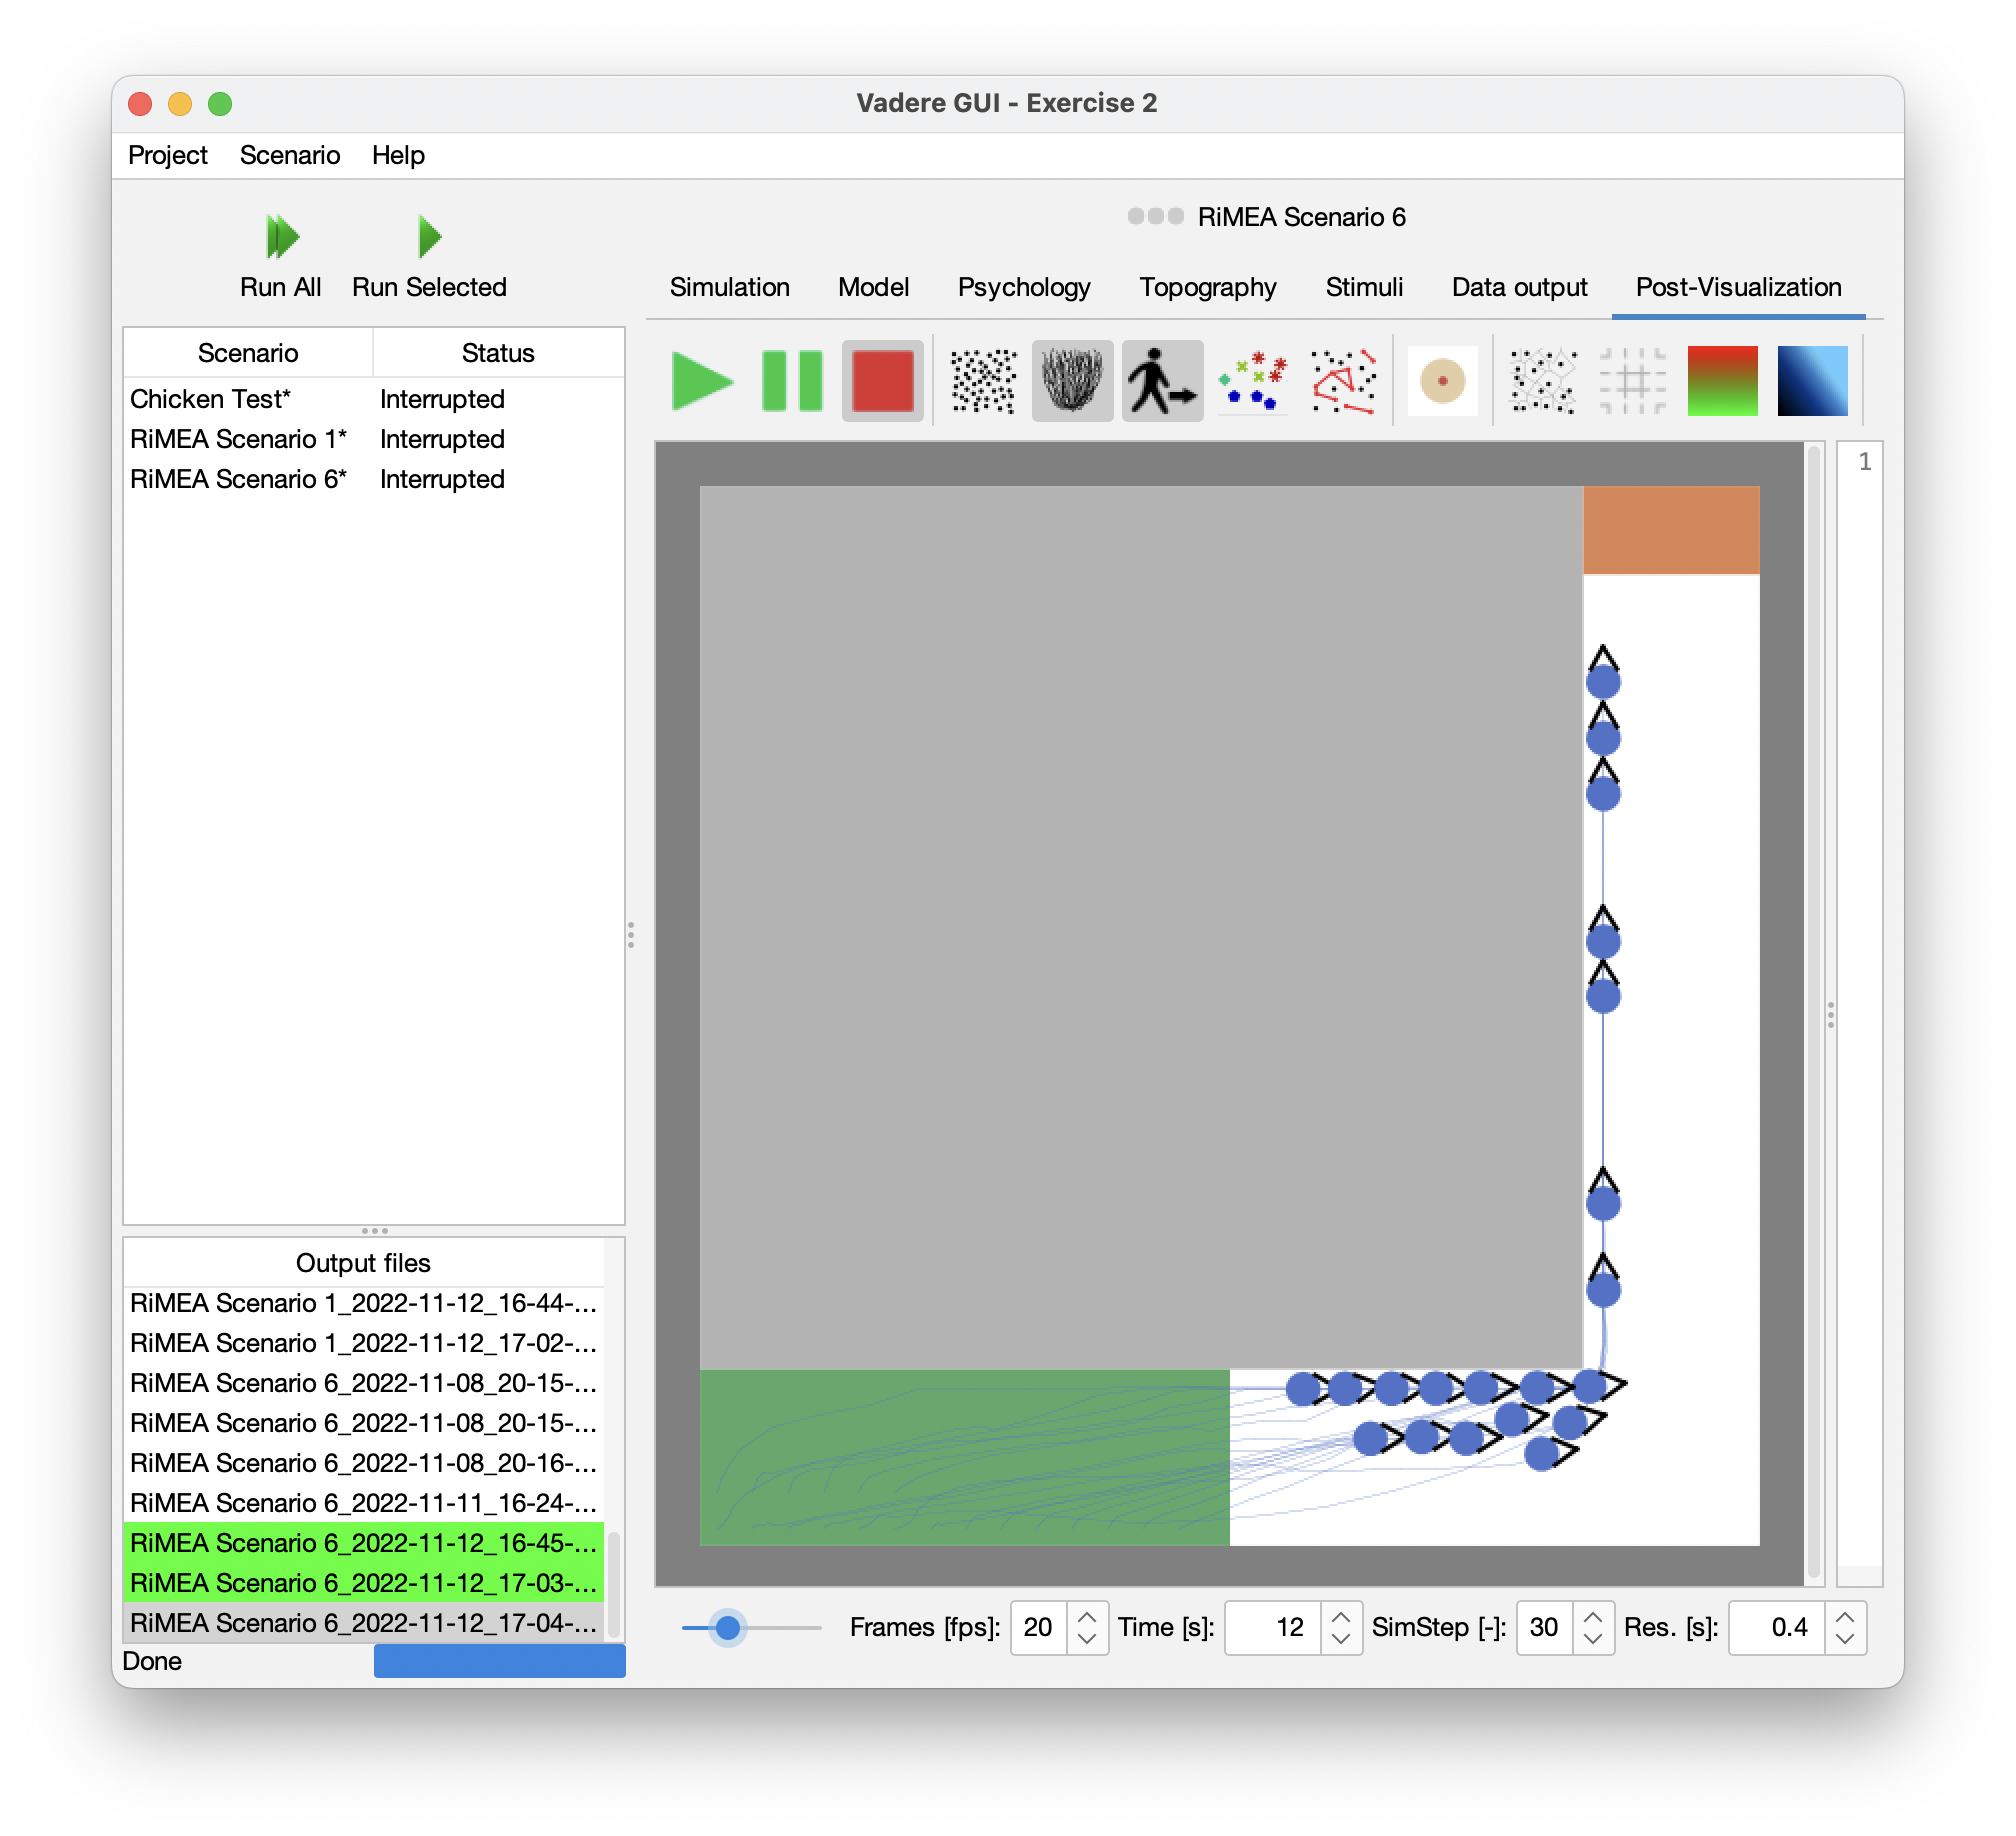
\includegraphics[width=0.33\textwidth]{images/gnm_6b.png}}
        \subfloat[At the end of the simulation]{
        \label{gnm_6c}
        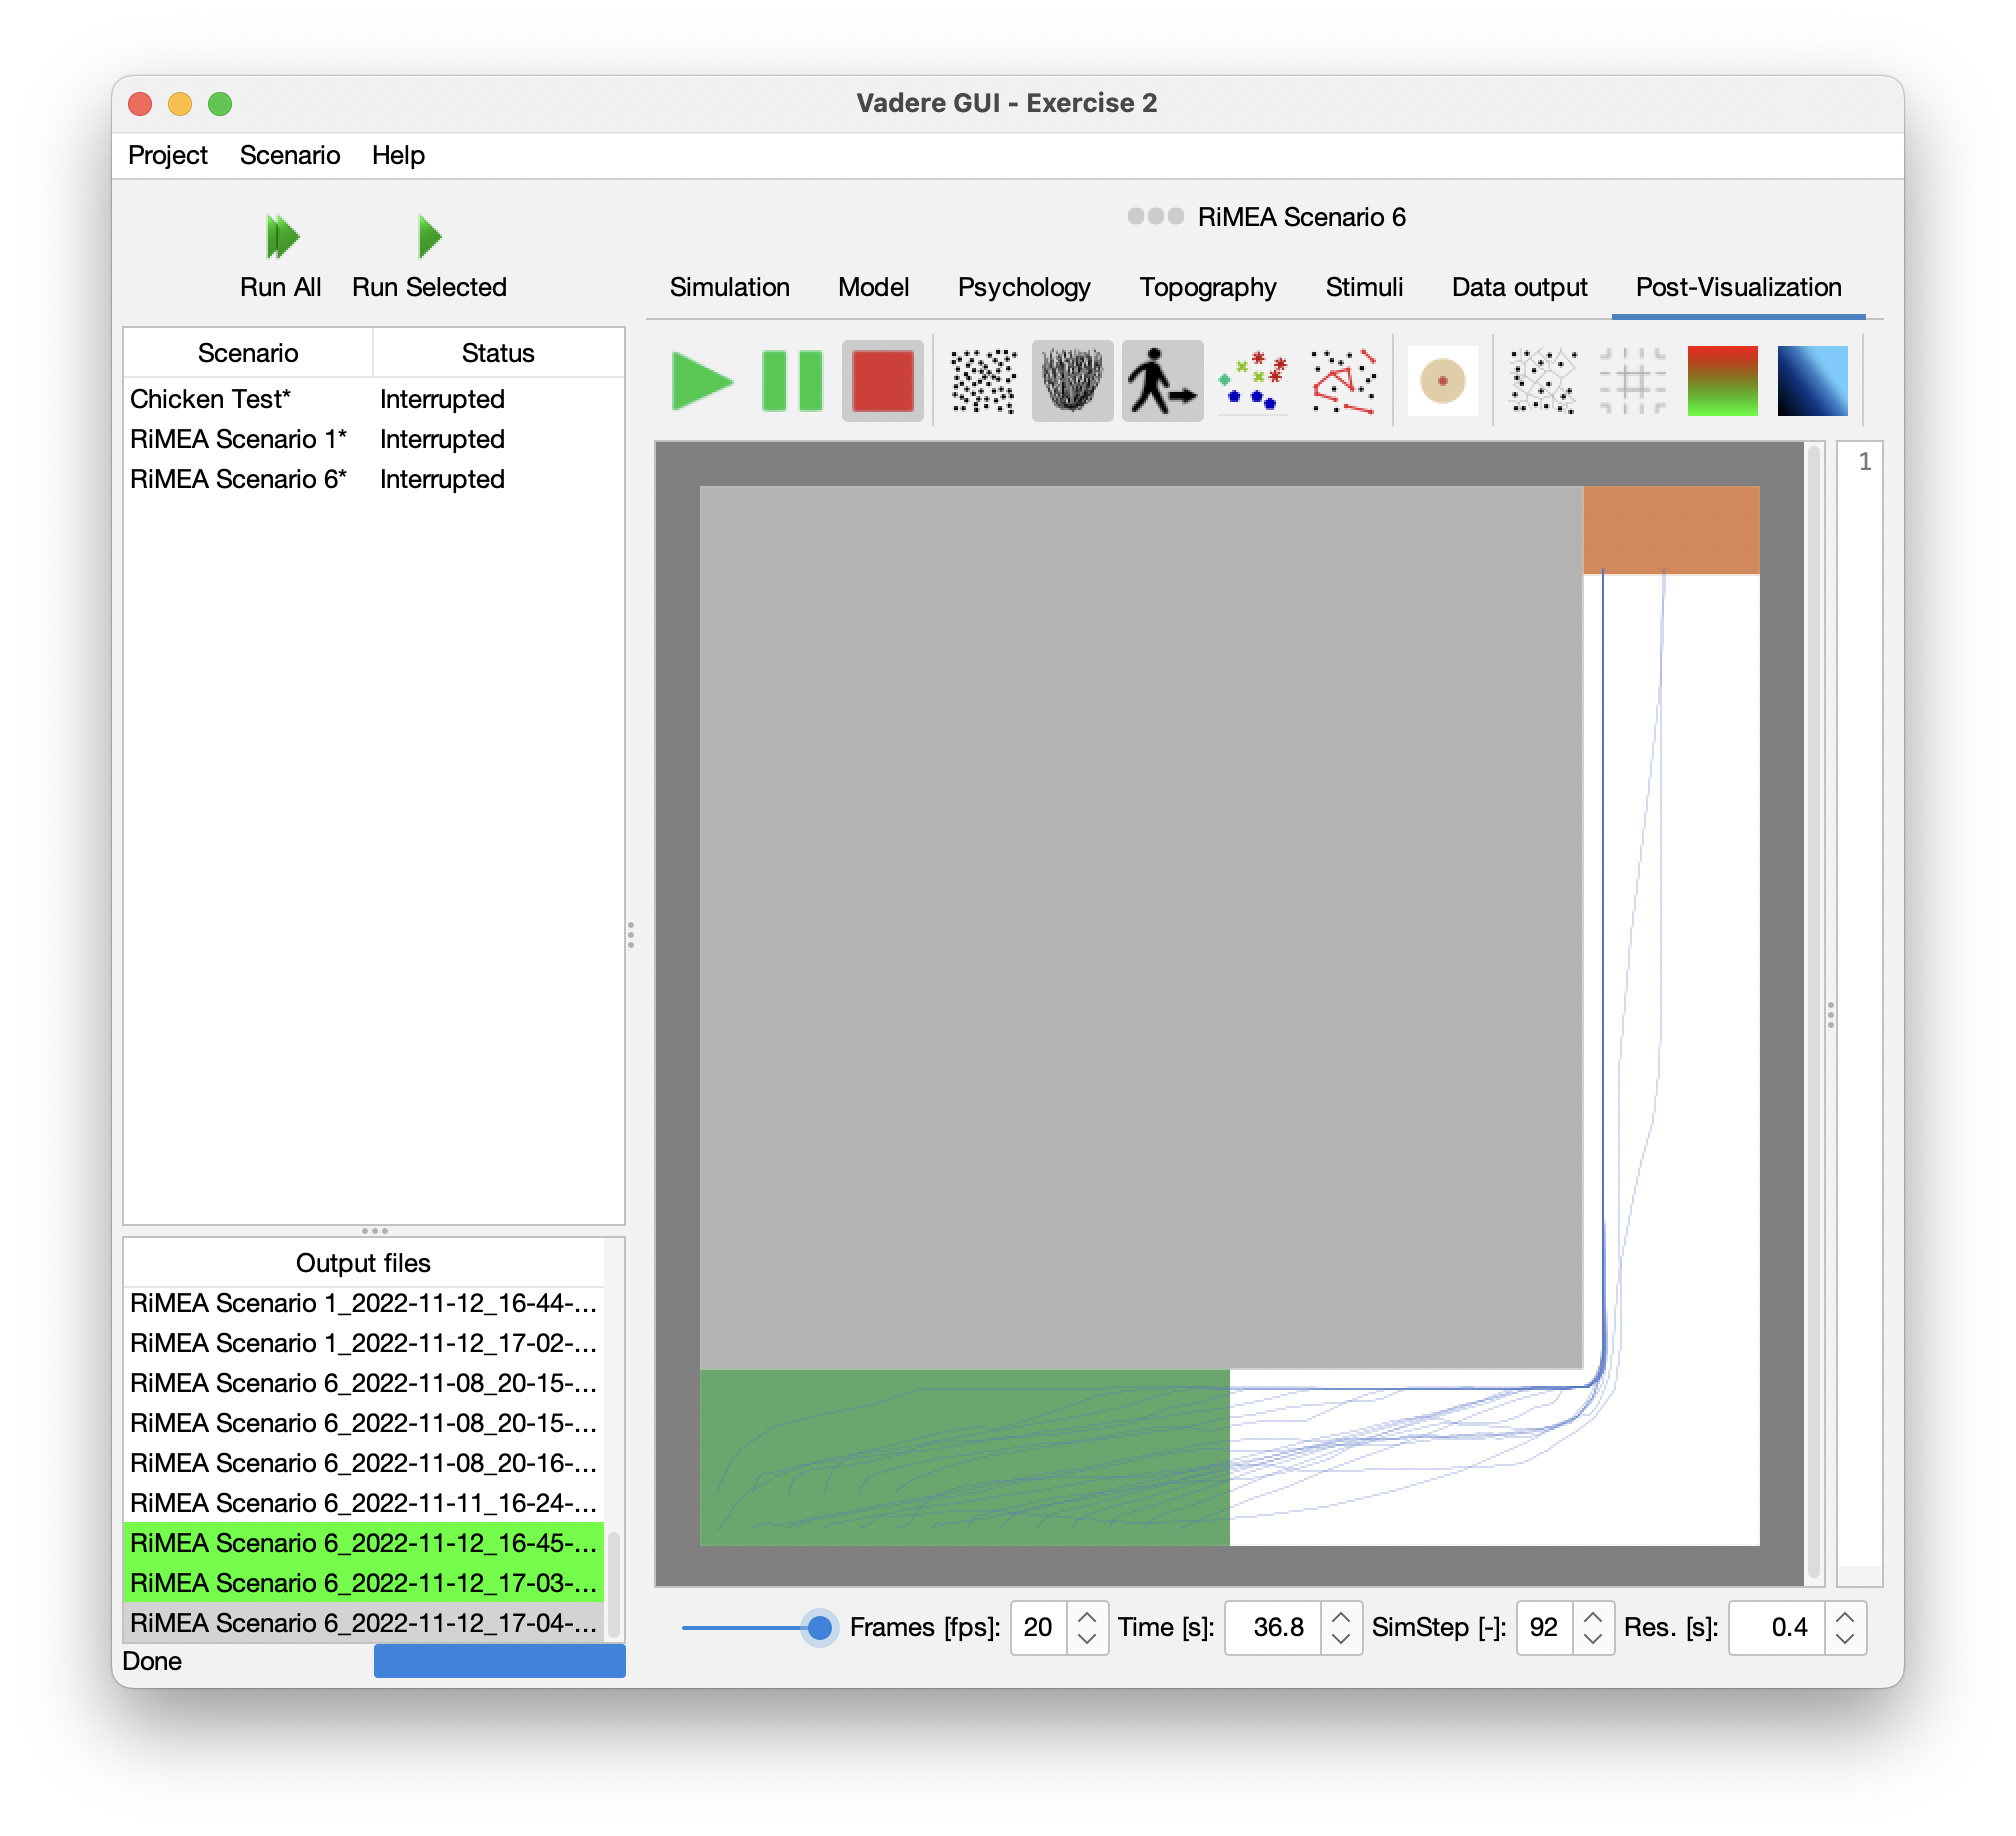
\includegraphics[width=0.33\textwidth]{images/gnm_6c.png}}
        \caption{Different stages of the simulation of the scenario 6 using the Gradient Navigation Model}
        \label{scenario6_gnm}
    \end{figure}
    
    \item Chicken test: in the chicken test, all pedestrians were able to turn around the U-shaped obstacle, by taking uniform paths as well. Their behaviour were similar to the described in the scenario 6, but this time different yet symmetrical paths were taken, depending on the starting point of each pedestrian inside the source (either slightly upper or lower). There were some exceptions as well, some pedestrians chose to avoid the obstructing pedestrians rather than waiting. This time, however, the travel time was reduced by around 6 seconds, most probably because in the simulation using OSM, the scattering of so many pedestrians in such narrow space for taking other paths caused a blockage, something that does not happen with GNM.
    
    \begin{figure} [H]
    \centering
    \subfloat[At the beginning of the simulation]{
        \label{gnm_chickena}
        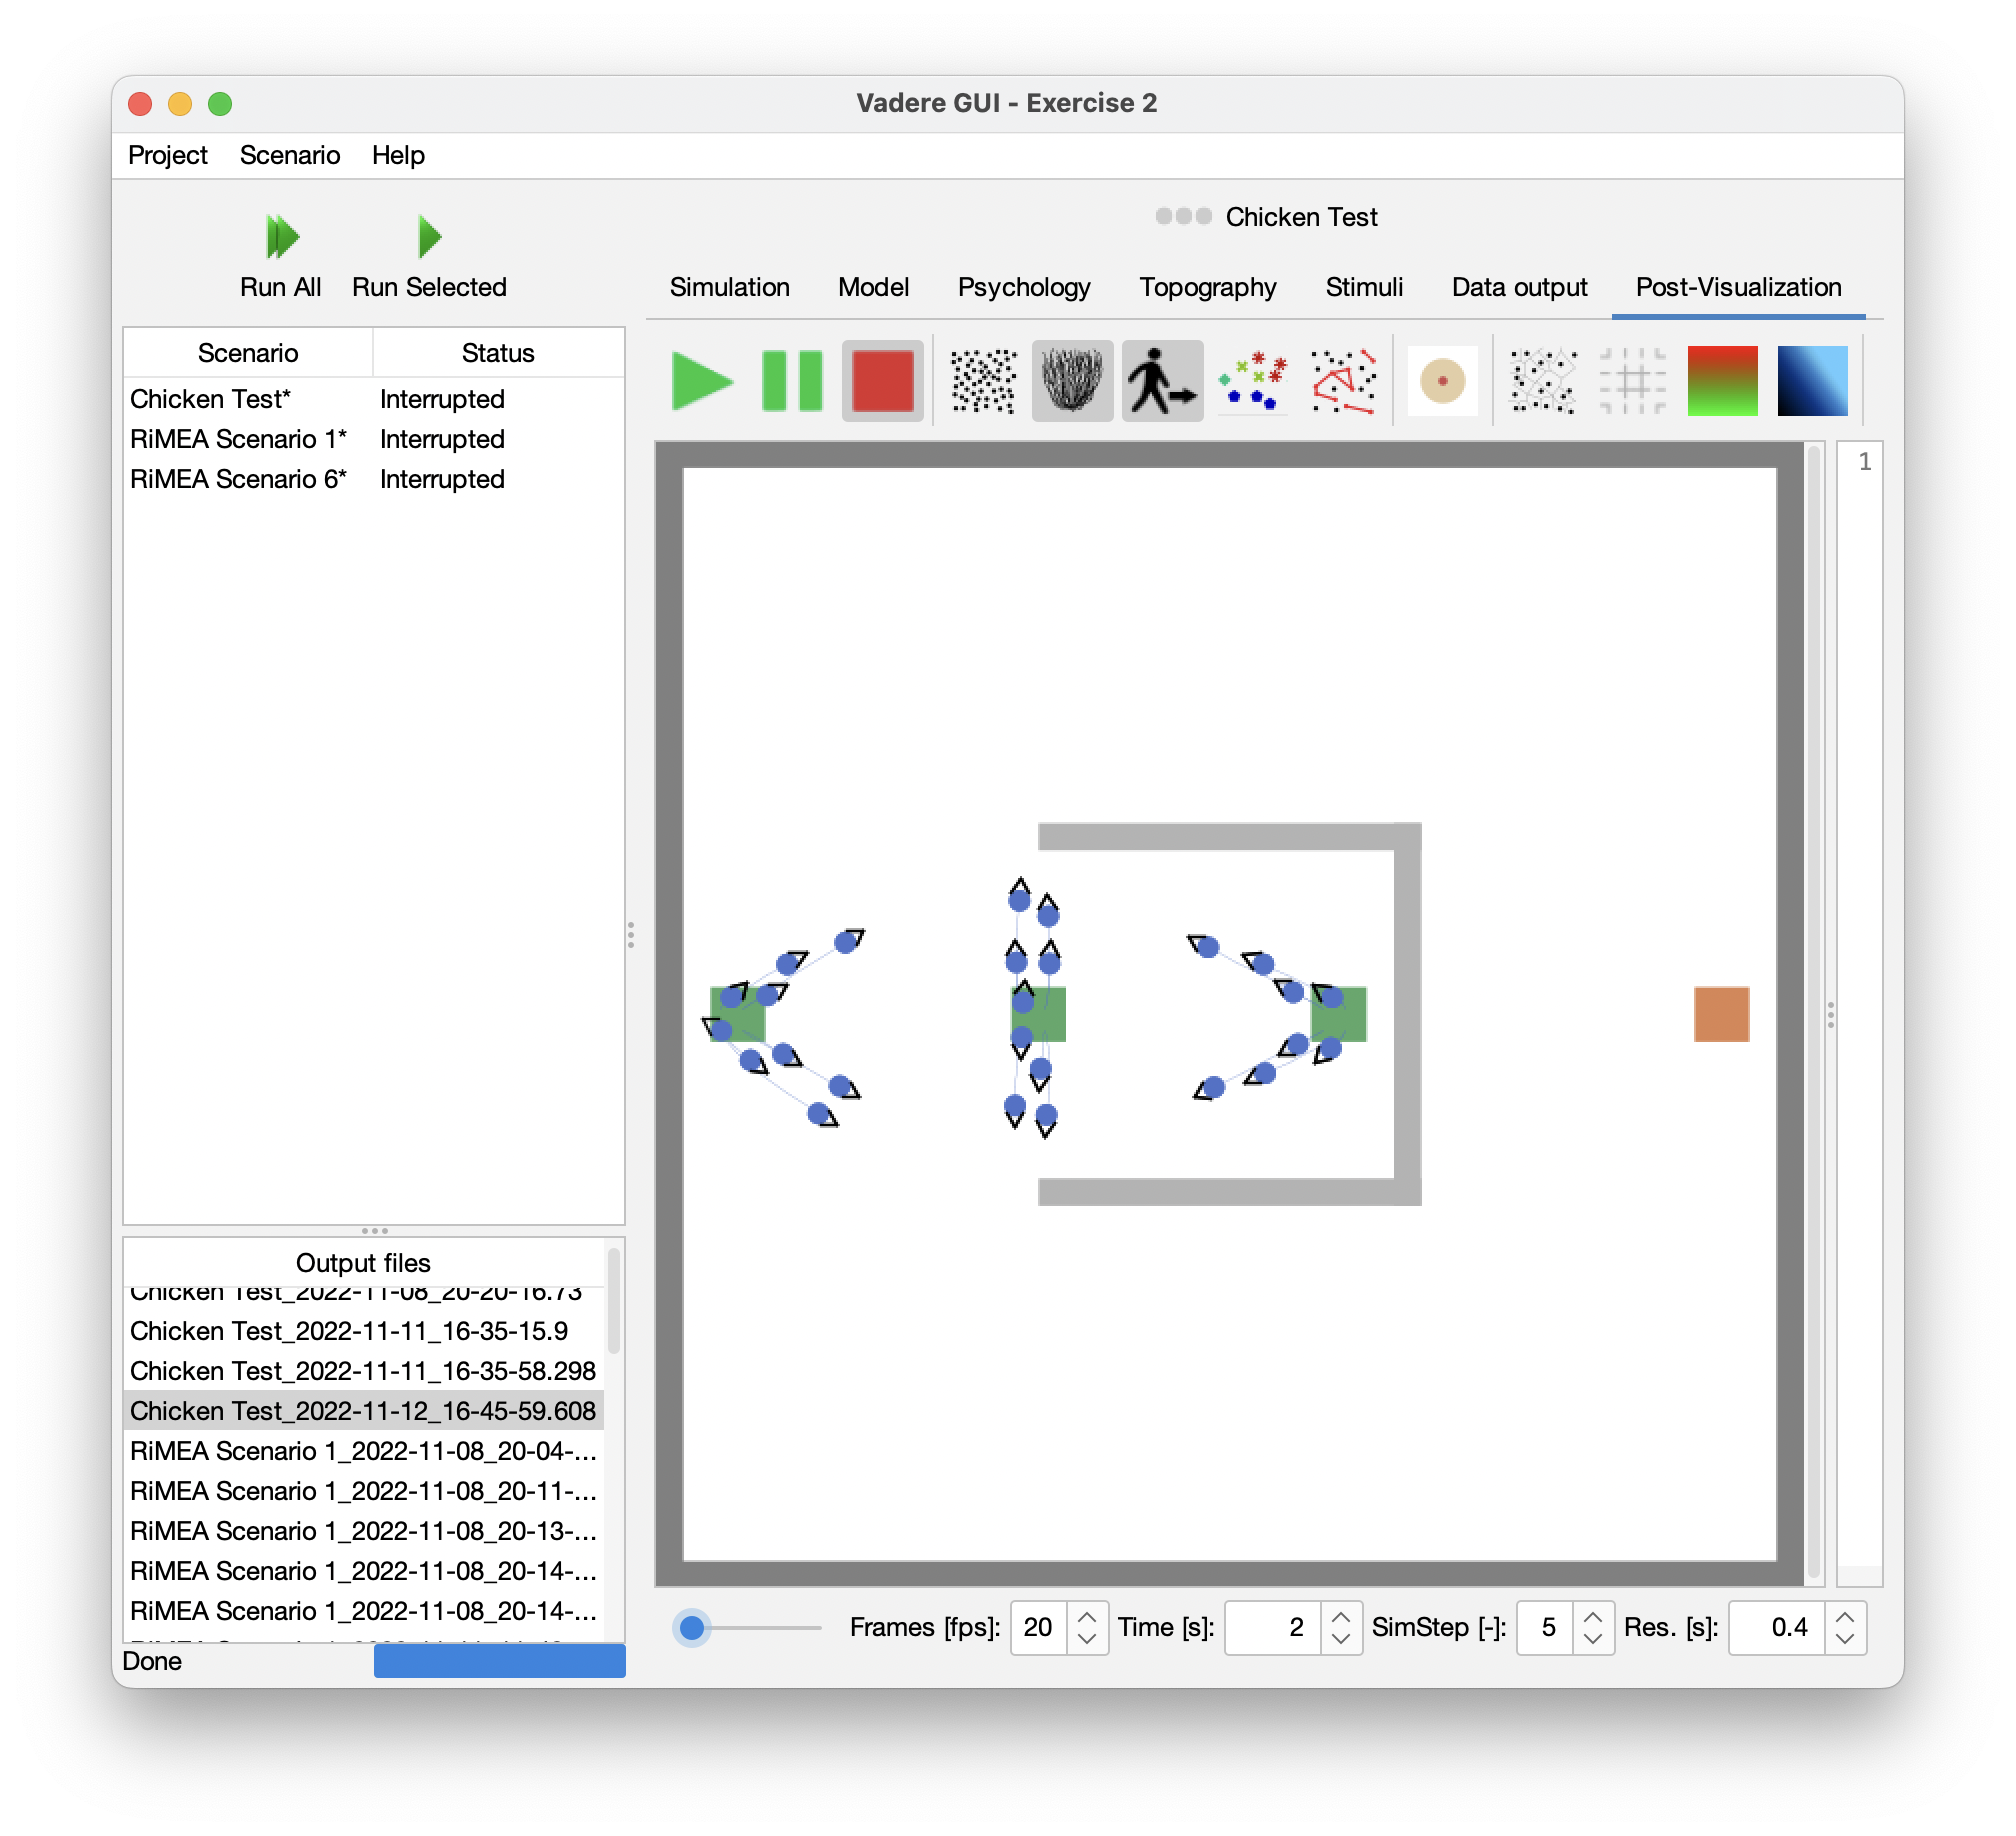
\includegraphics[width=0.33\textwidth]{images/gnm_chickena.png}}
        \subfloat[In the middle of the simulation]{
        \label{gnm_chickenb}
        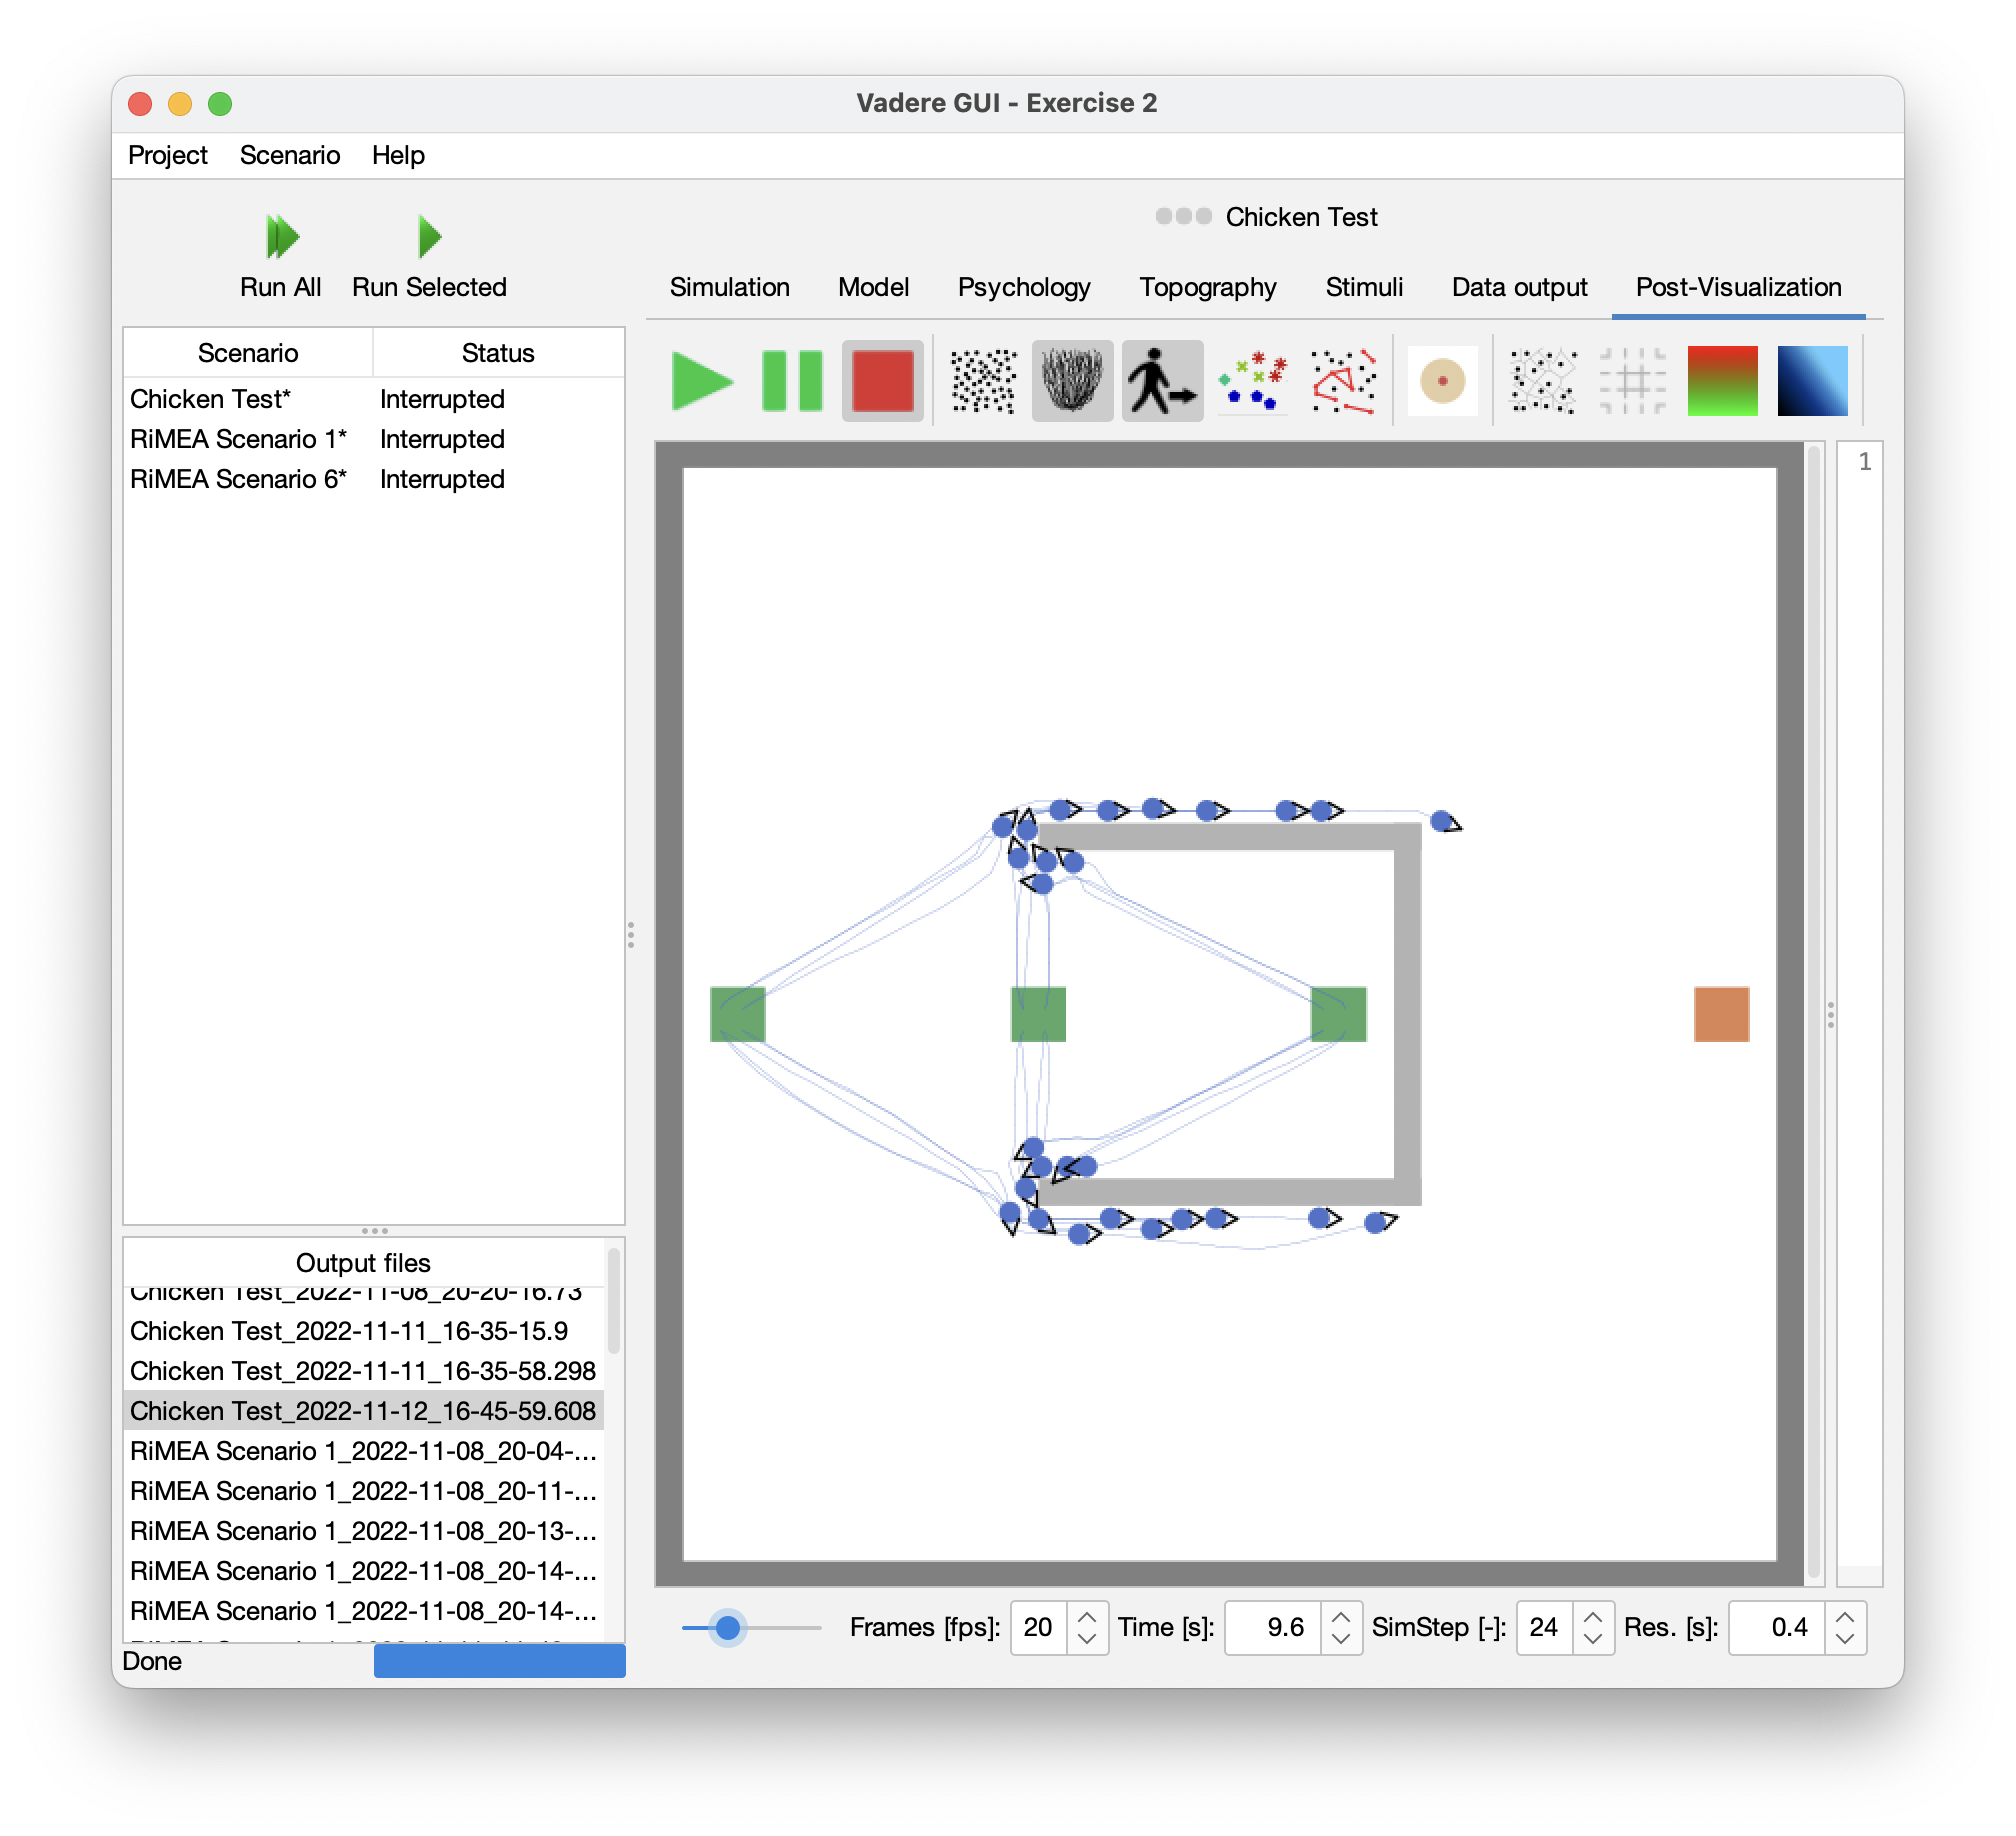
\includegraphics[width=0.33\textwidth]{images/gnm_chickenb.png}}
        \subfloat[At the end of the simulation]{
        \label{gnm_chickenc}
        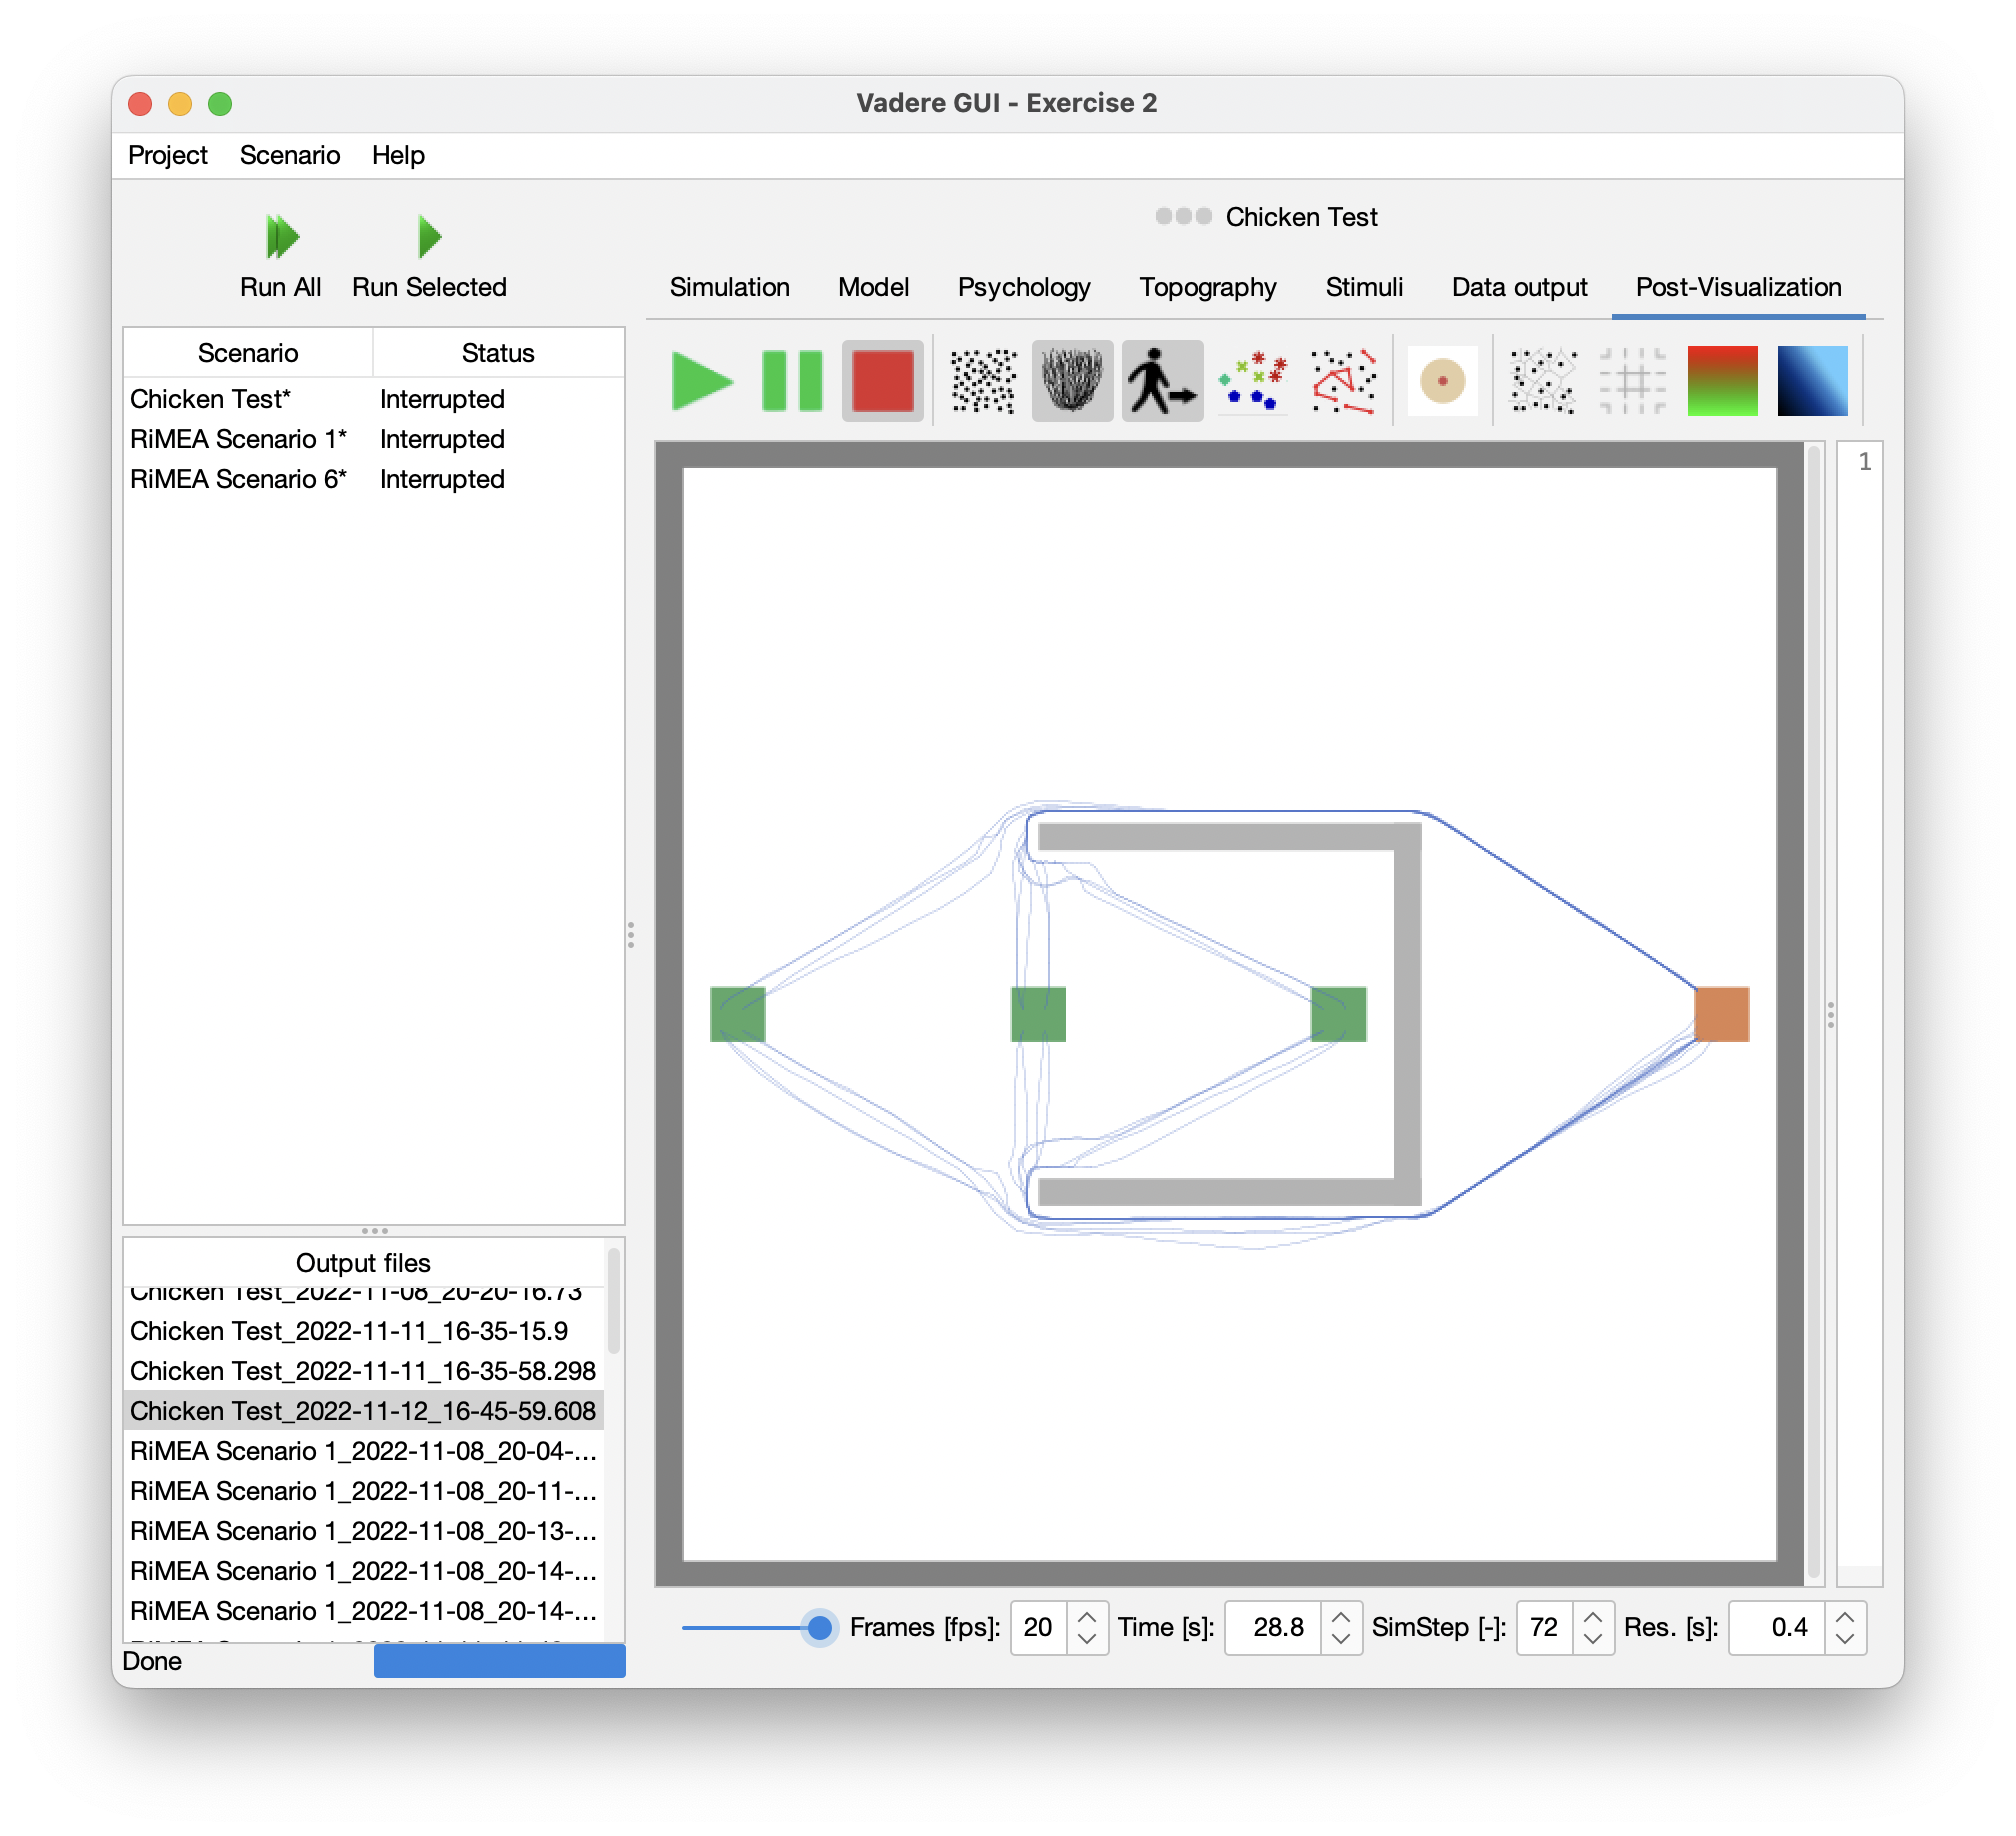
\includegraphics[width=0.33\textwidth]{images/gnm_chickenc.png}}
        \caption{Different stages of the simulation of the chicken test using the Gradient Navigation Model}
        \label{chicken_gnm}
    \end{figure}
    
\end{enumerate}
    

\bigskip

\noindent{\textbf{Joint analysis}}

After looking through the results of the simulation of the previous three scenarios using the different models, it can be concluded that the change of models affected specially the way the paths were distributed. The directions taken by the pedestrians in each scenario were similar, but the main difference lain in the level of strictness in terms of ``path bifurcation" they had to follow while traversing it, meaning that the more strict the model, the less the pedestrians were allowed to take other paths in order to avoid other pedestrians. The OSM is the less strict, whereas the GNM is the most, as can be noticed in the comparisons in Figures \ref{comparison_scenario6} and \ref{comparison_chickentest}.

    \begin{figure} [H]
    \centering
    \subfloat[Optimal Steps Model]{
        \label{scenario_6}
        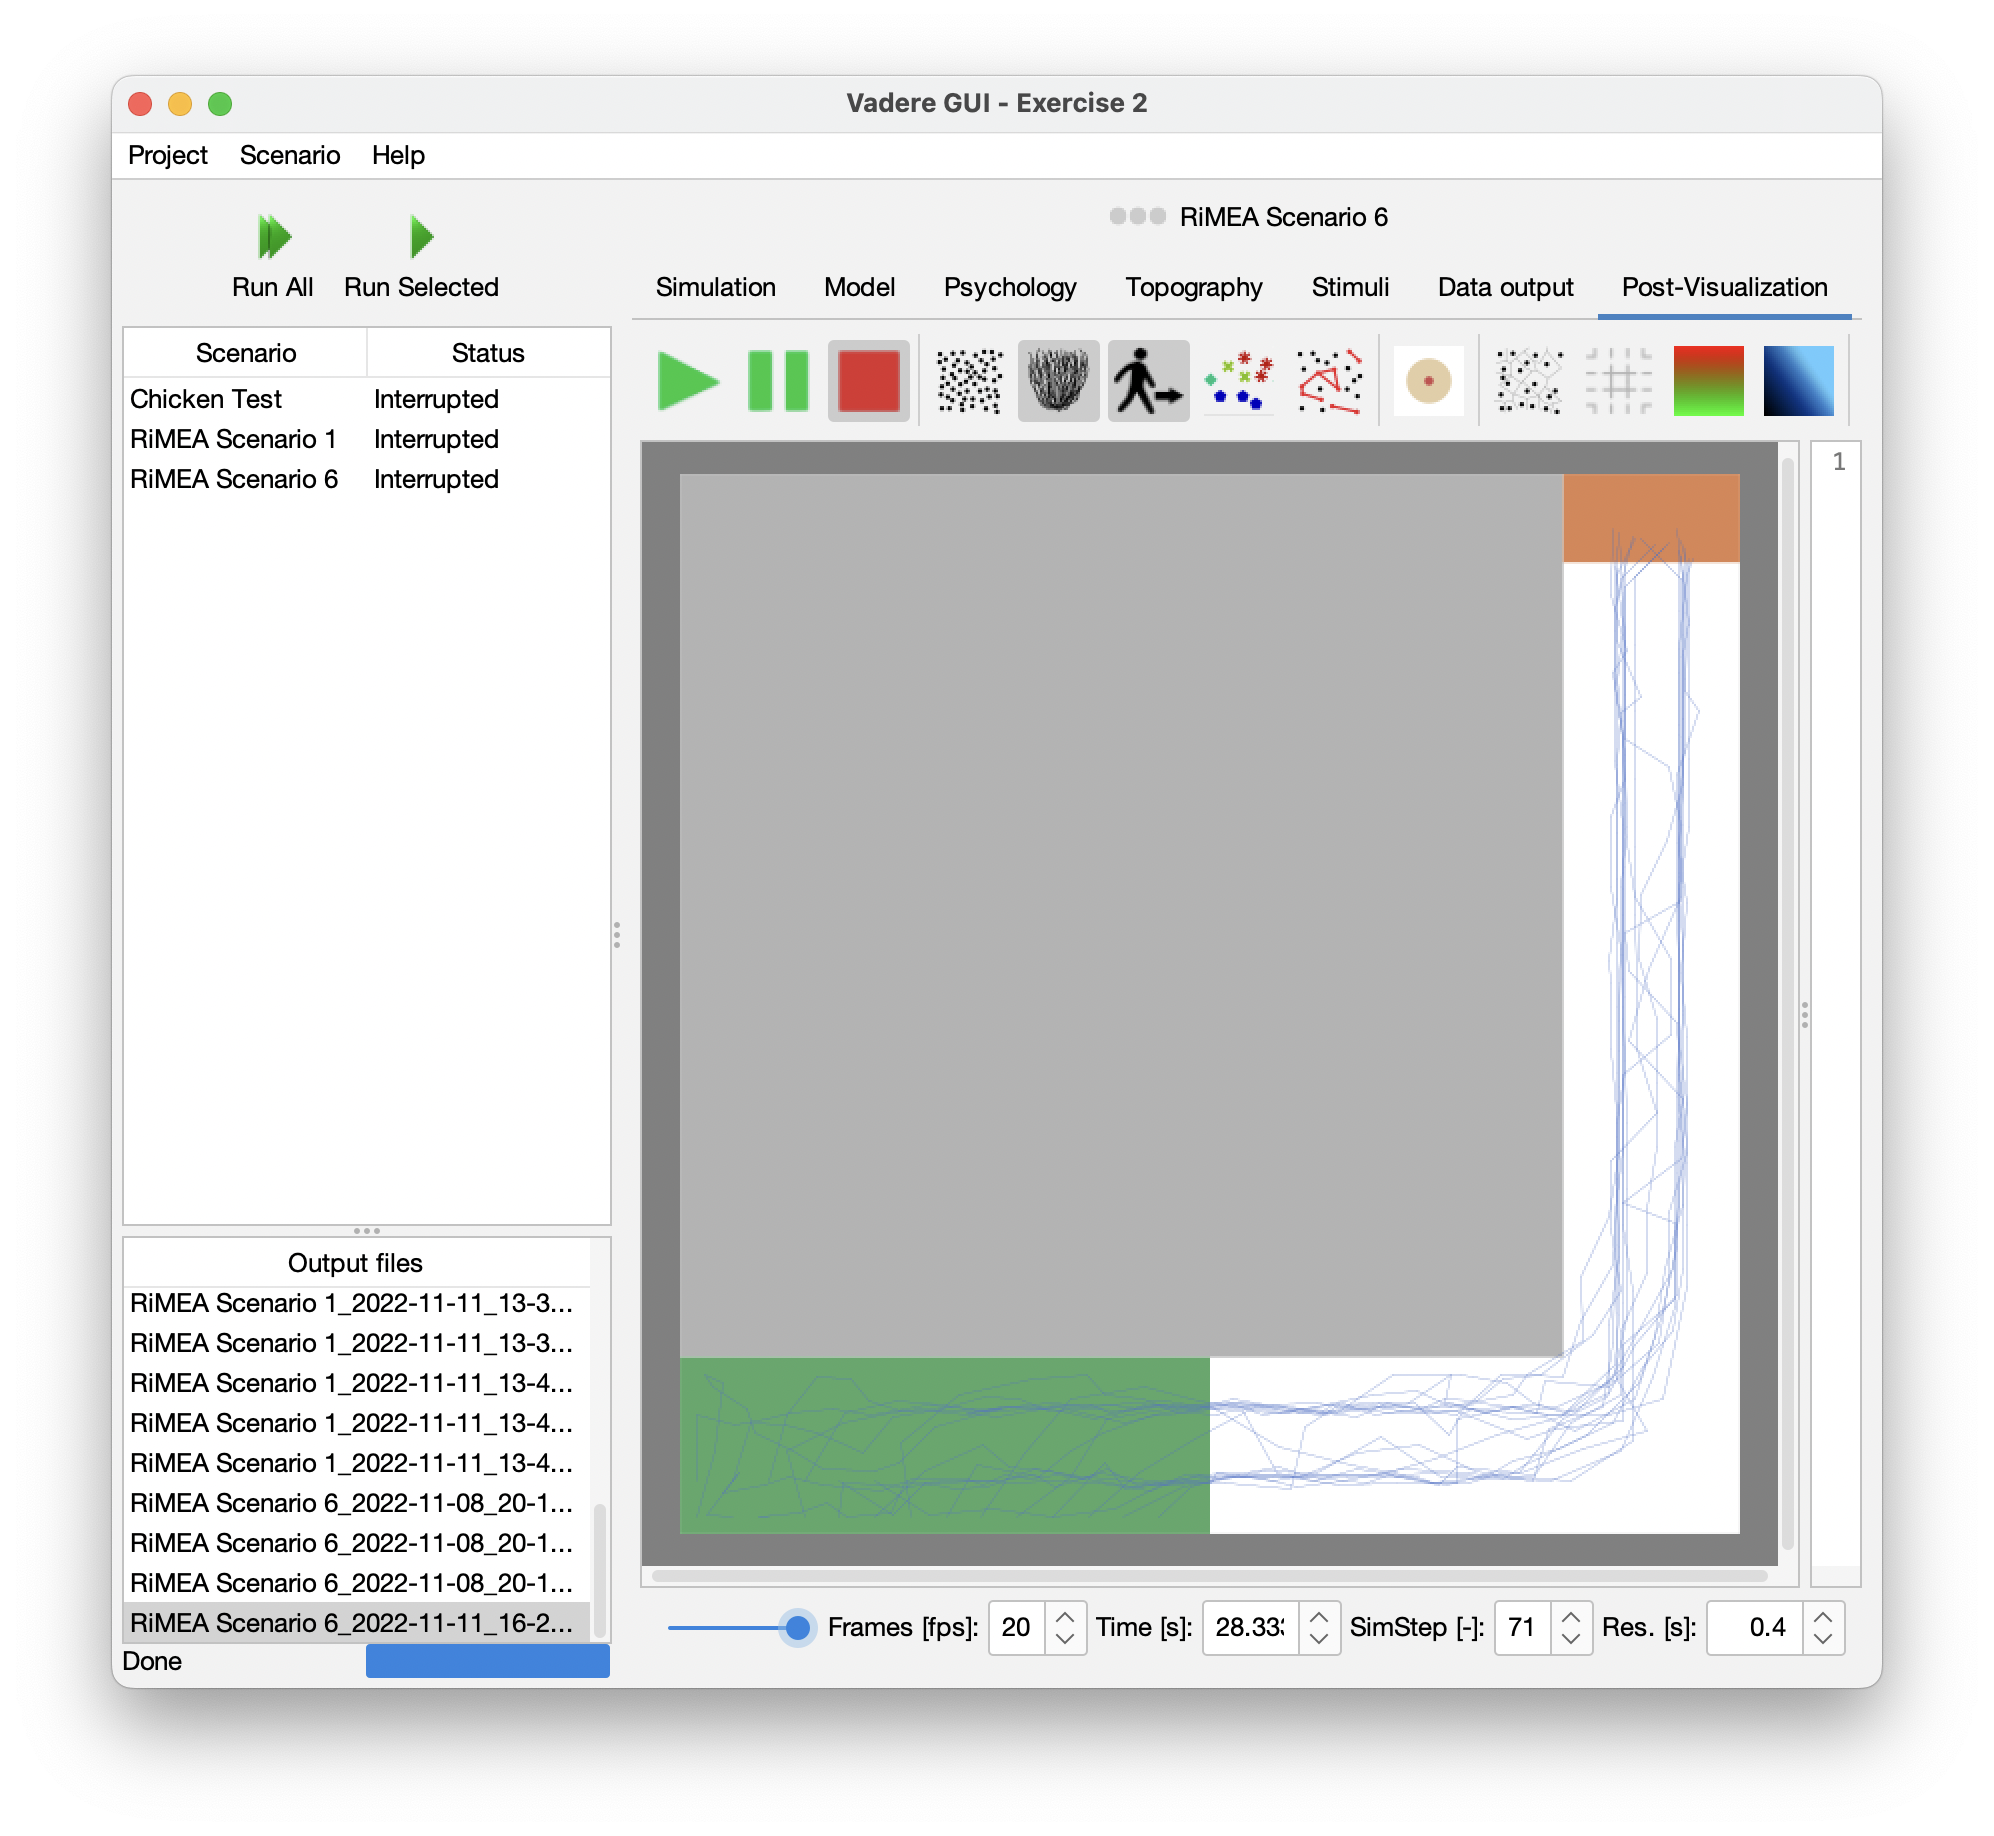
\includegraphics[width=0.33\textwidth]{images/scenario_6c.png}}
        \subfloat[Social Force Model]{
        \label{sfm_6c}
        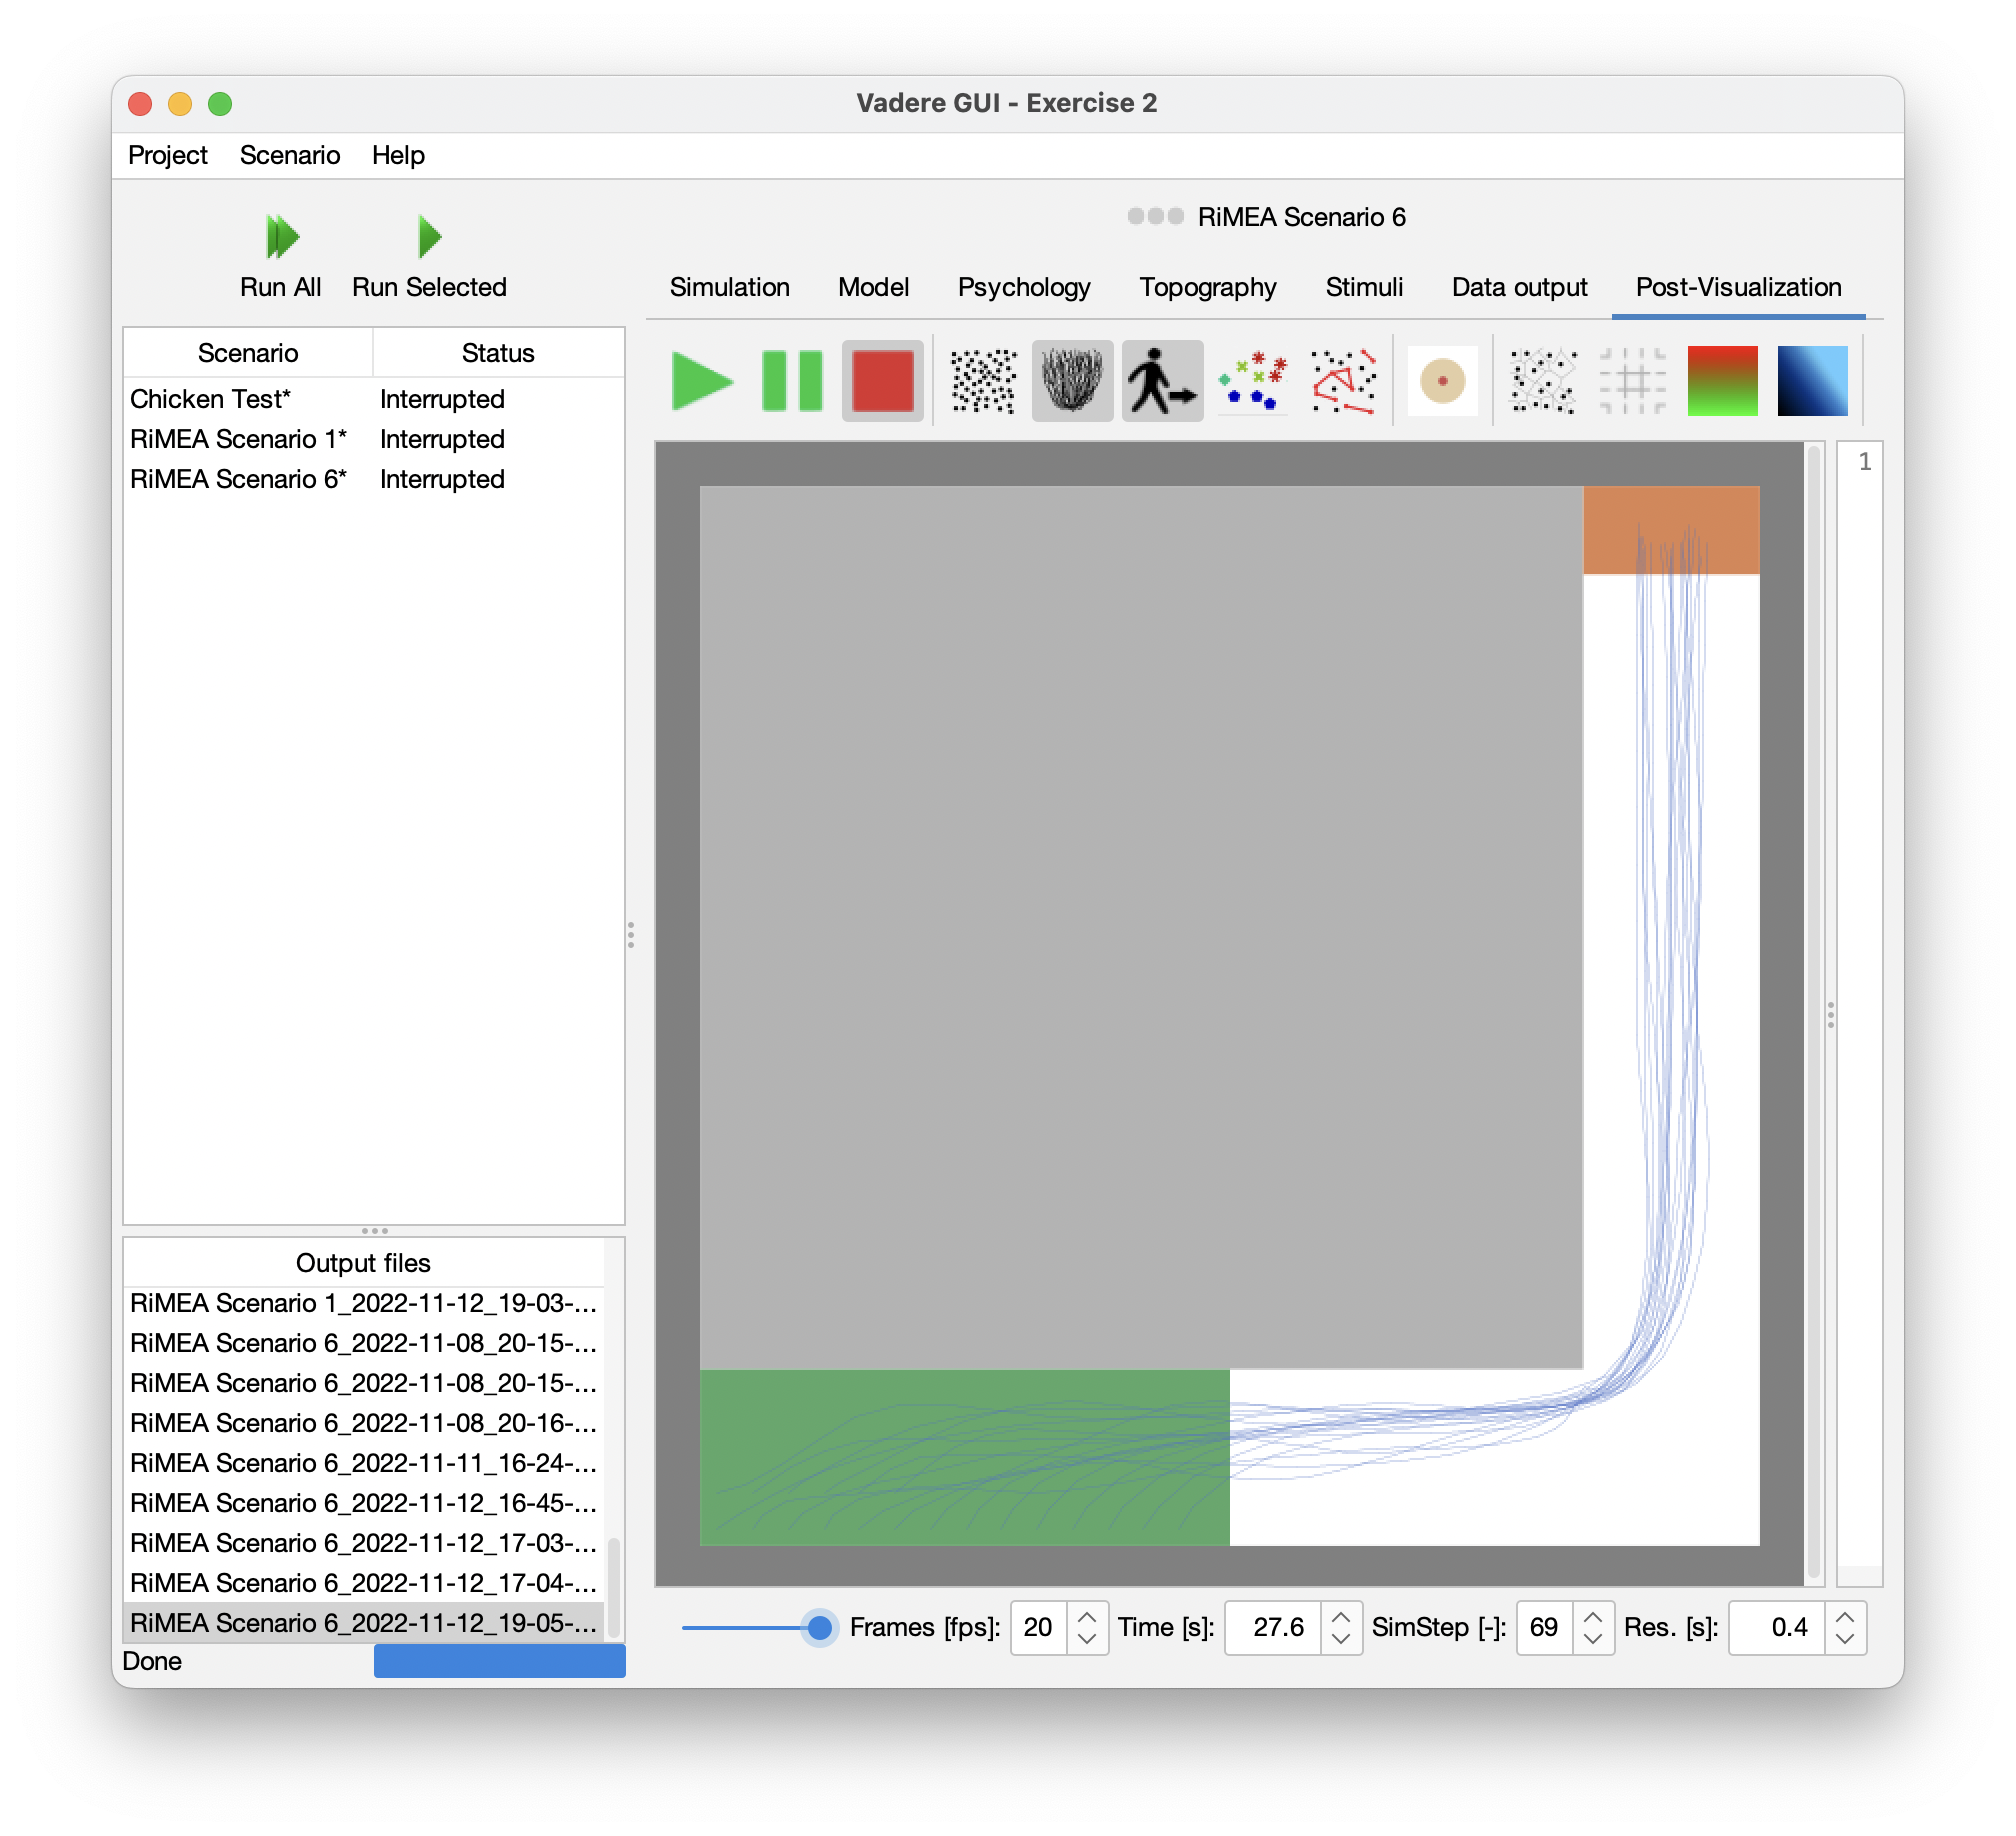
\includegraphics[width=0.33\textwidth]{images/sfm_6c.png}}
        \subfloat[Gradient Navigation Model]{
        \label{gnm_6c}
        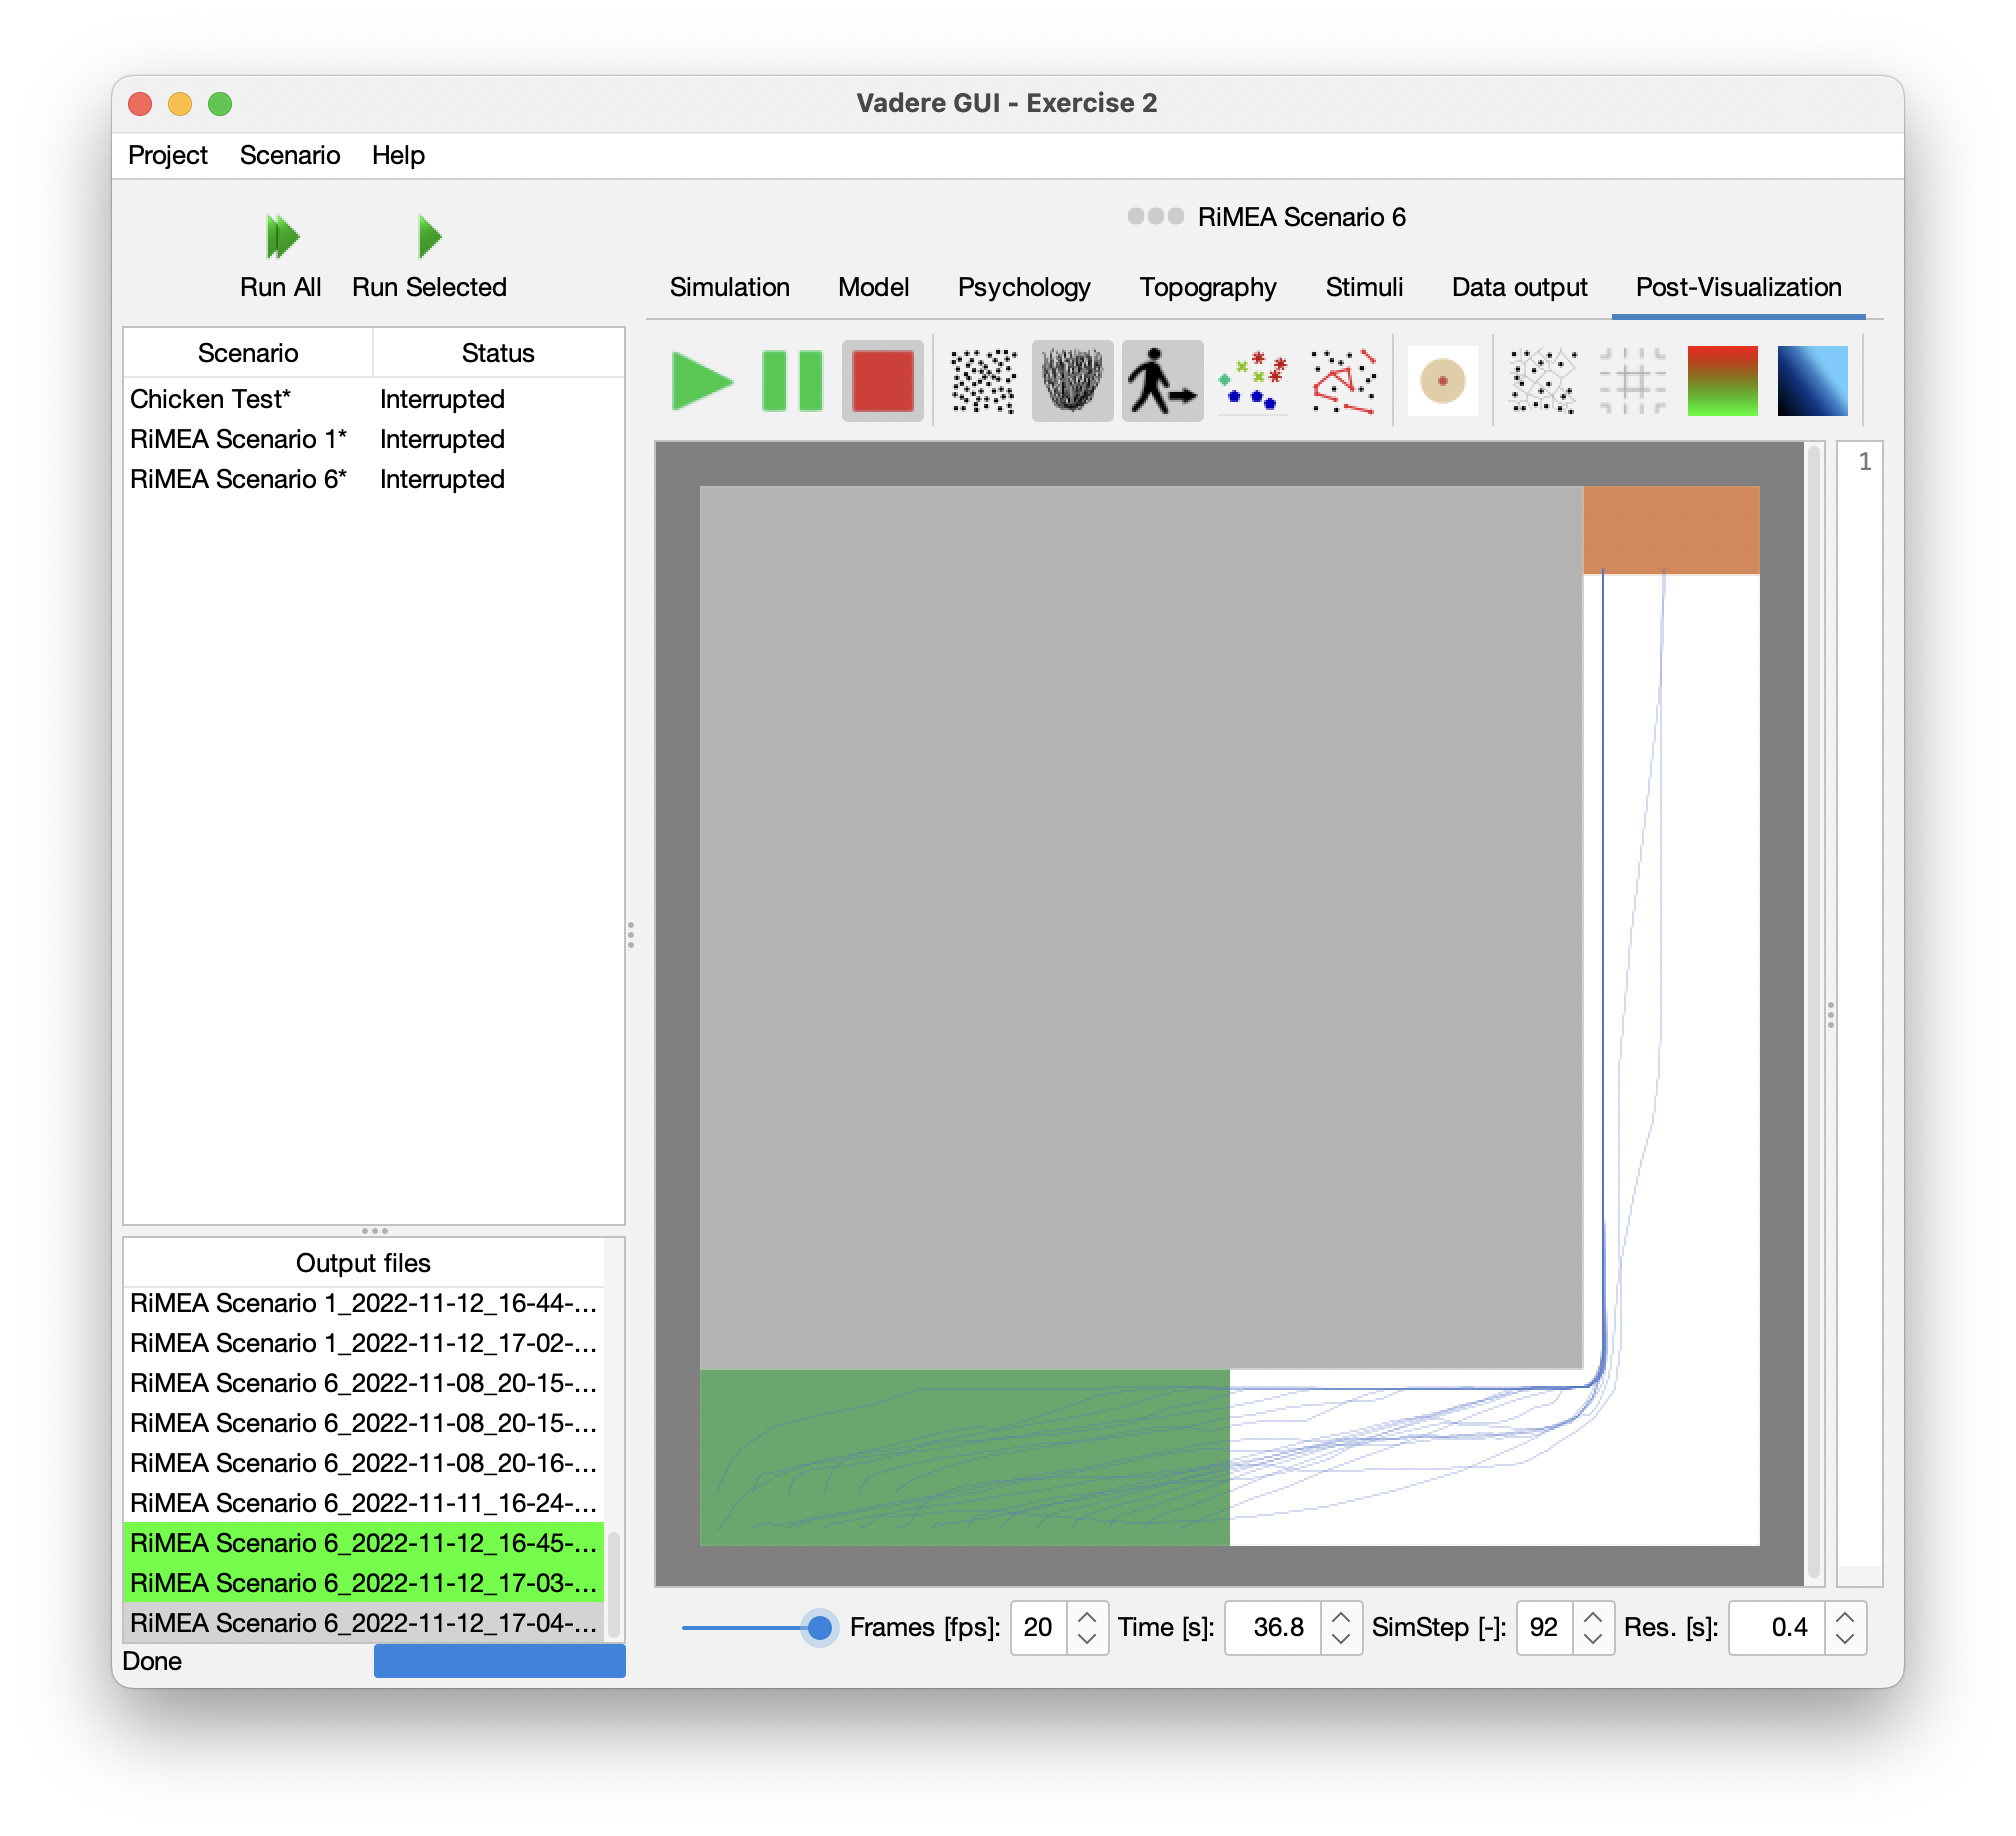
\includegraphics[width=0.33\textwidth]{images/gnm_6c.png}}
        \caption{Comparison of the scenario 6 between the 3 models}
        \label{comparison_scenario6}
    \end{figure}

    \begin{figure} [H]
    \centering
    \subfloat[Optimal Steps Model]{
        \label{chicken_c}
        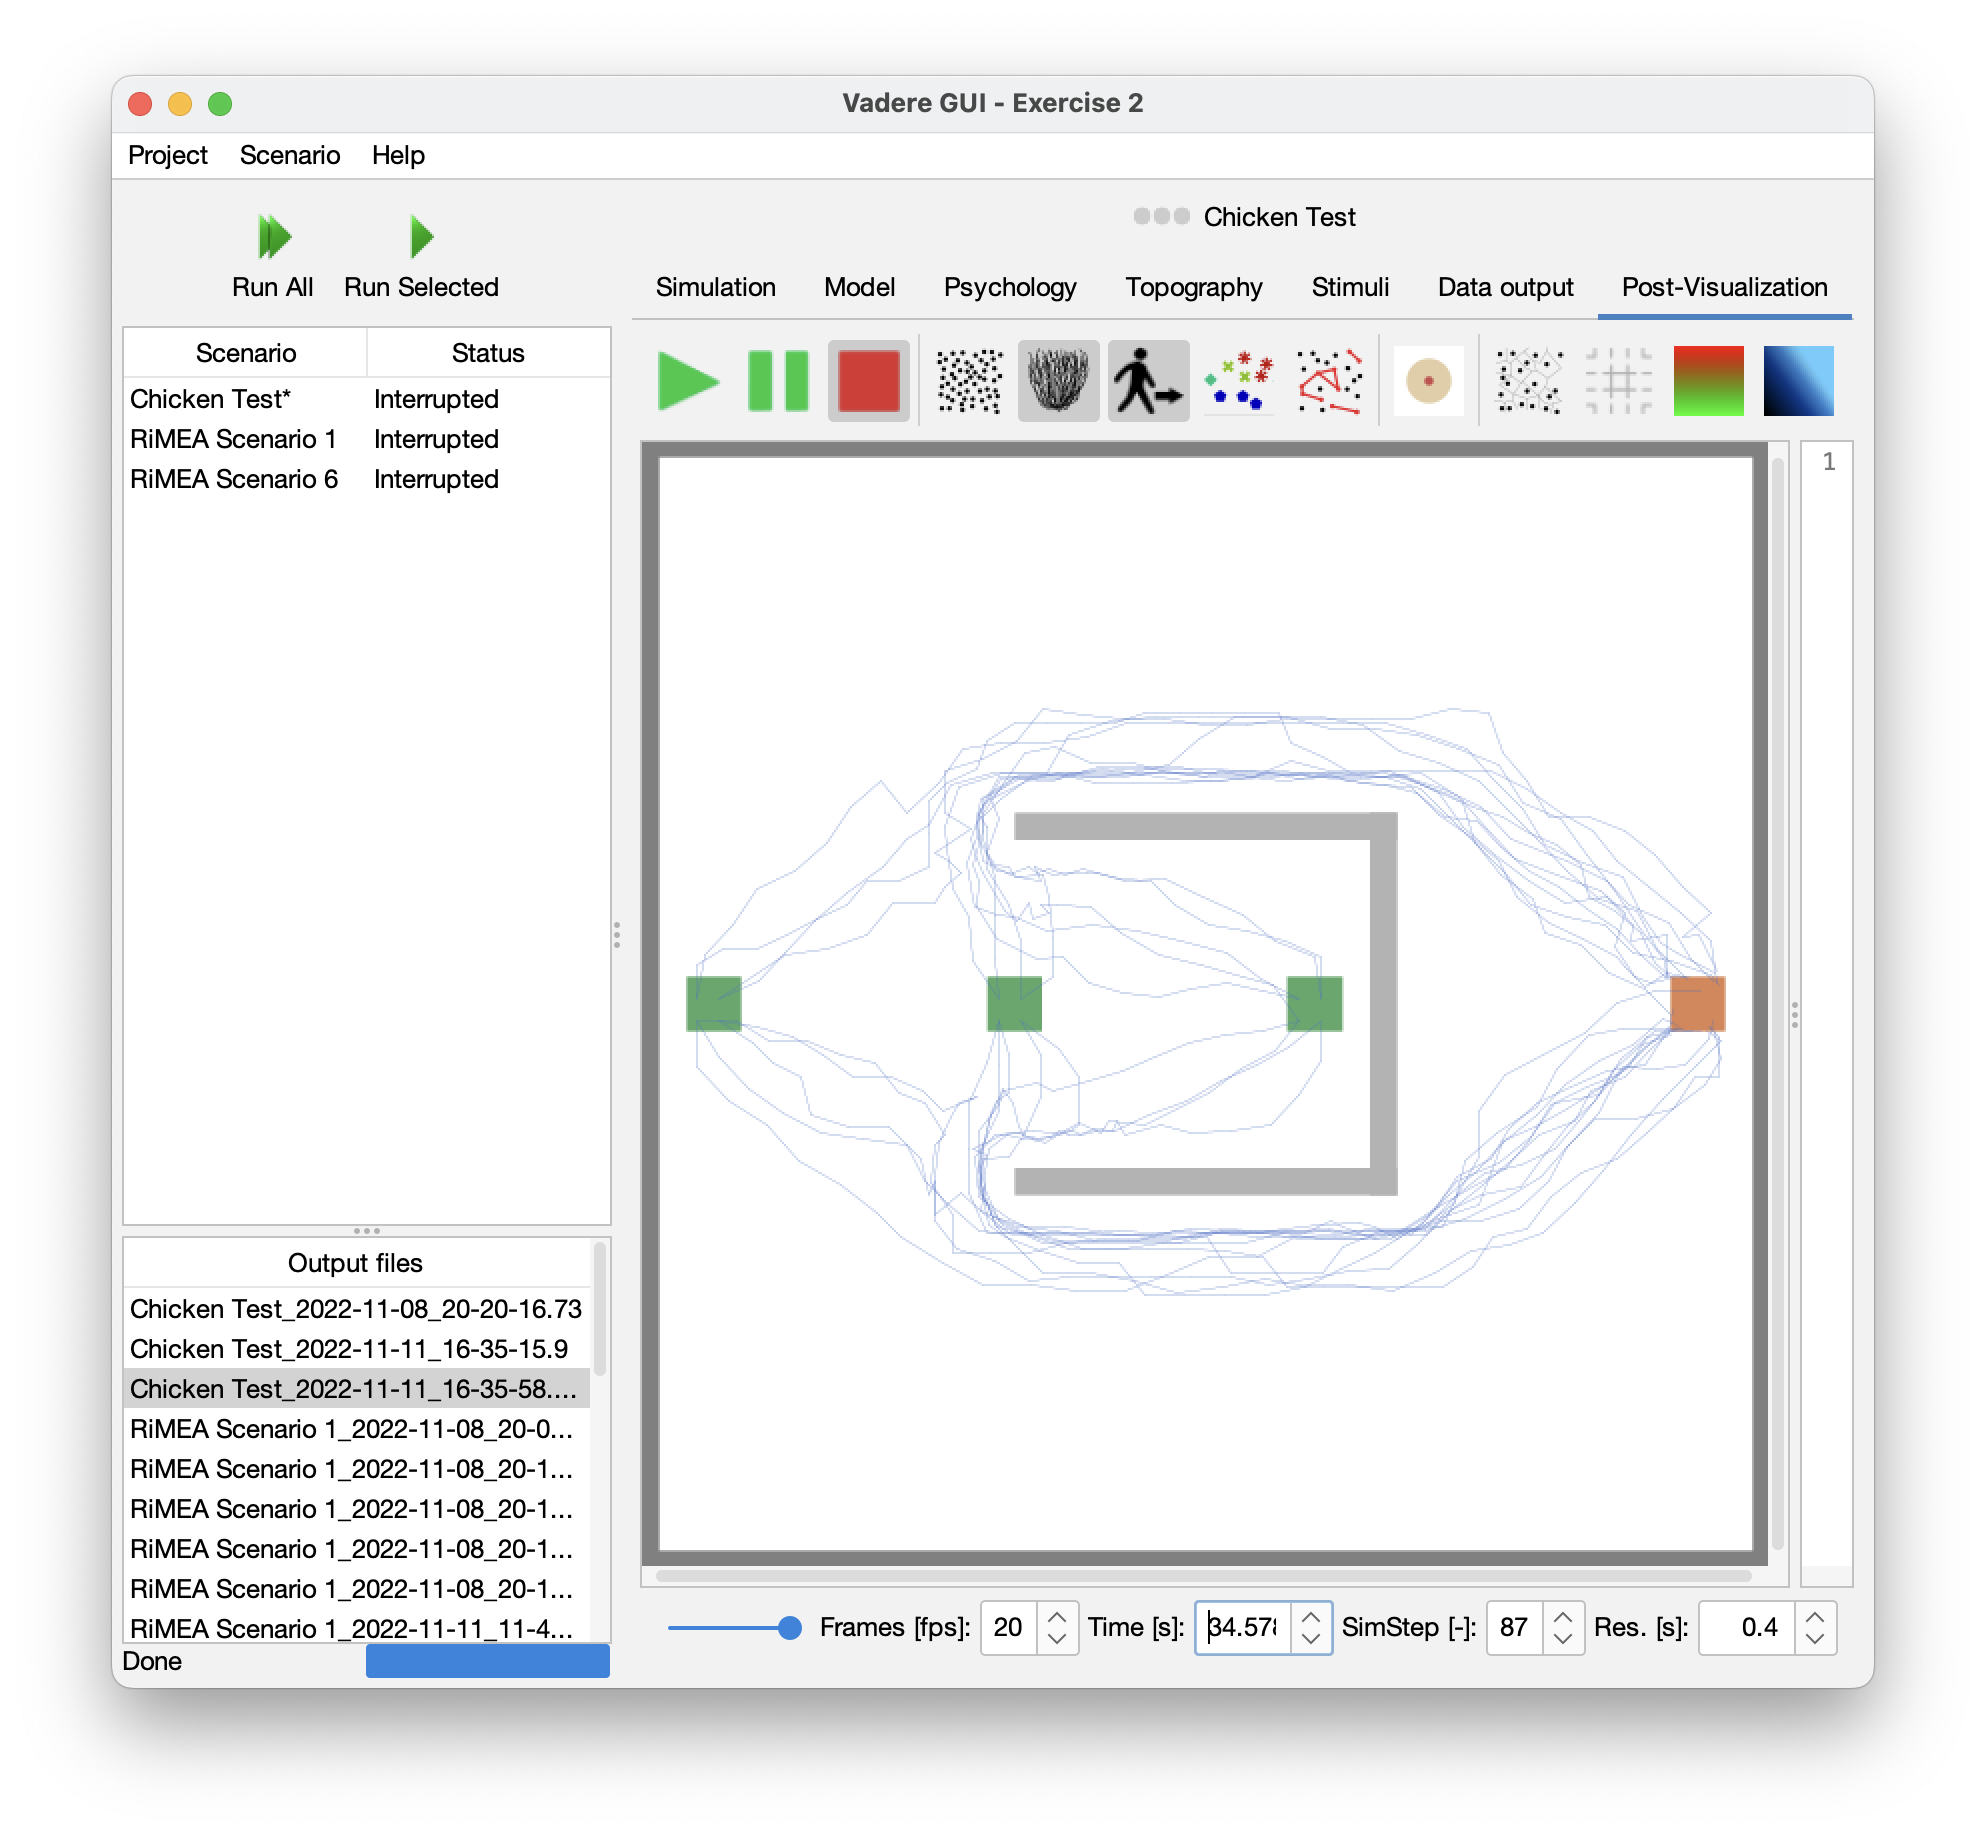
\includegraphics[width=0.33\textwidth]{images/chicken_c.png}}
        \subfloat[Social Force Model]{
        \label{sfm_chickenc}
        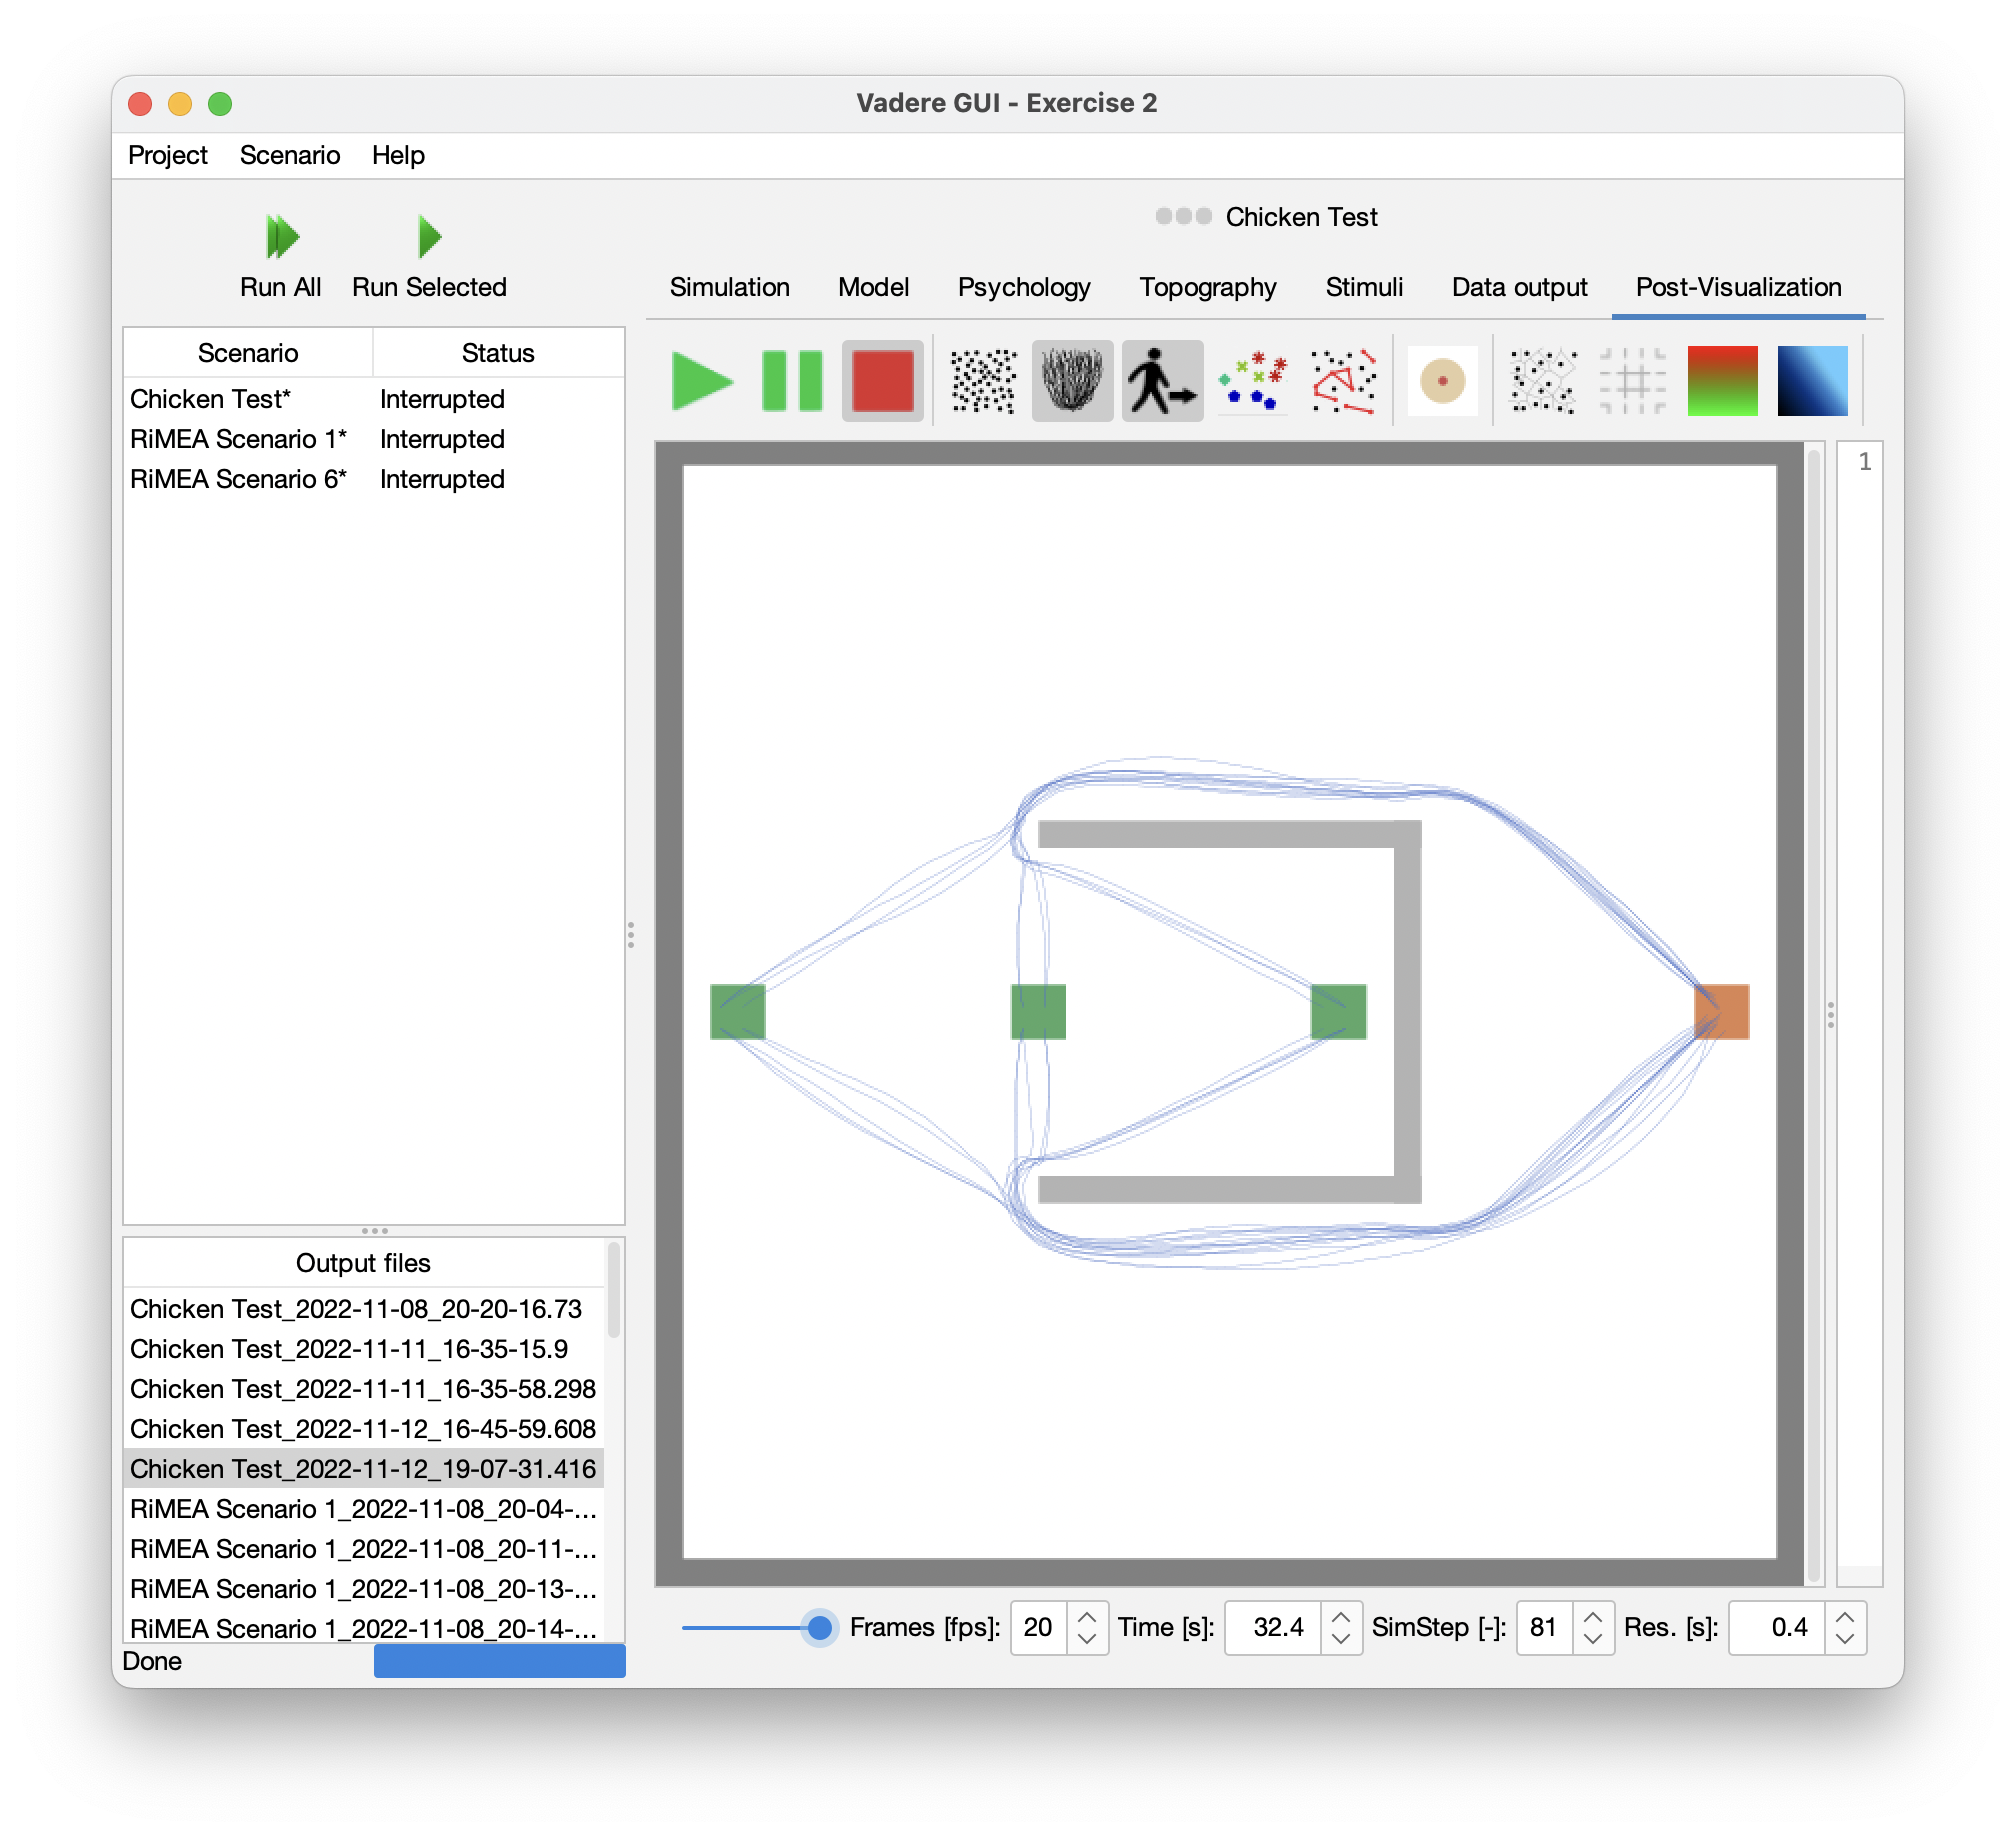
\includegraphics[width=0.33\textwidth]{images/sfm_chickenc.png}}
        \subfloat[Gradient Navigation Model]{
        \label{gnm_chickenc}
        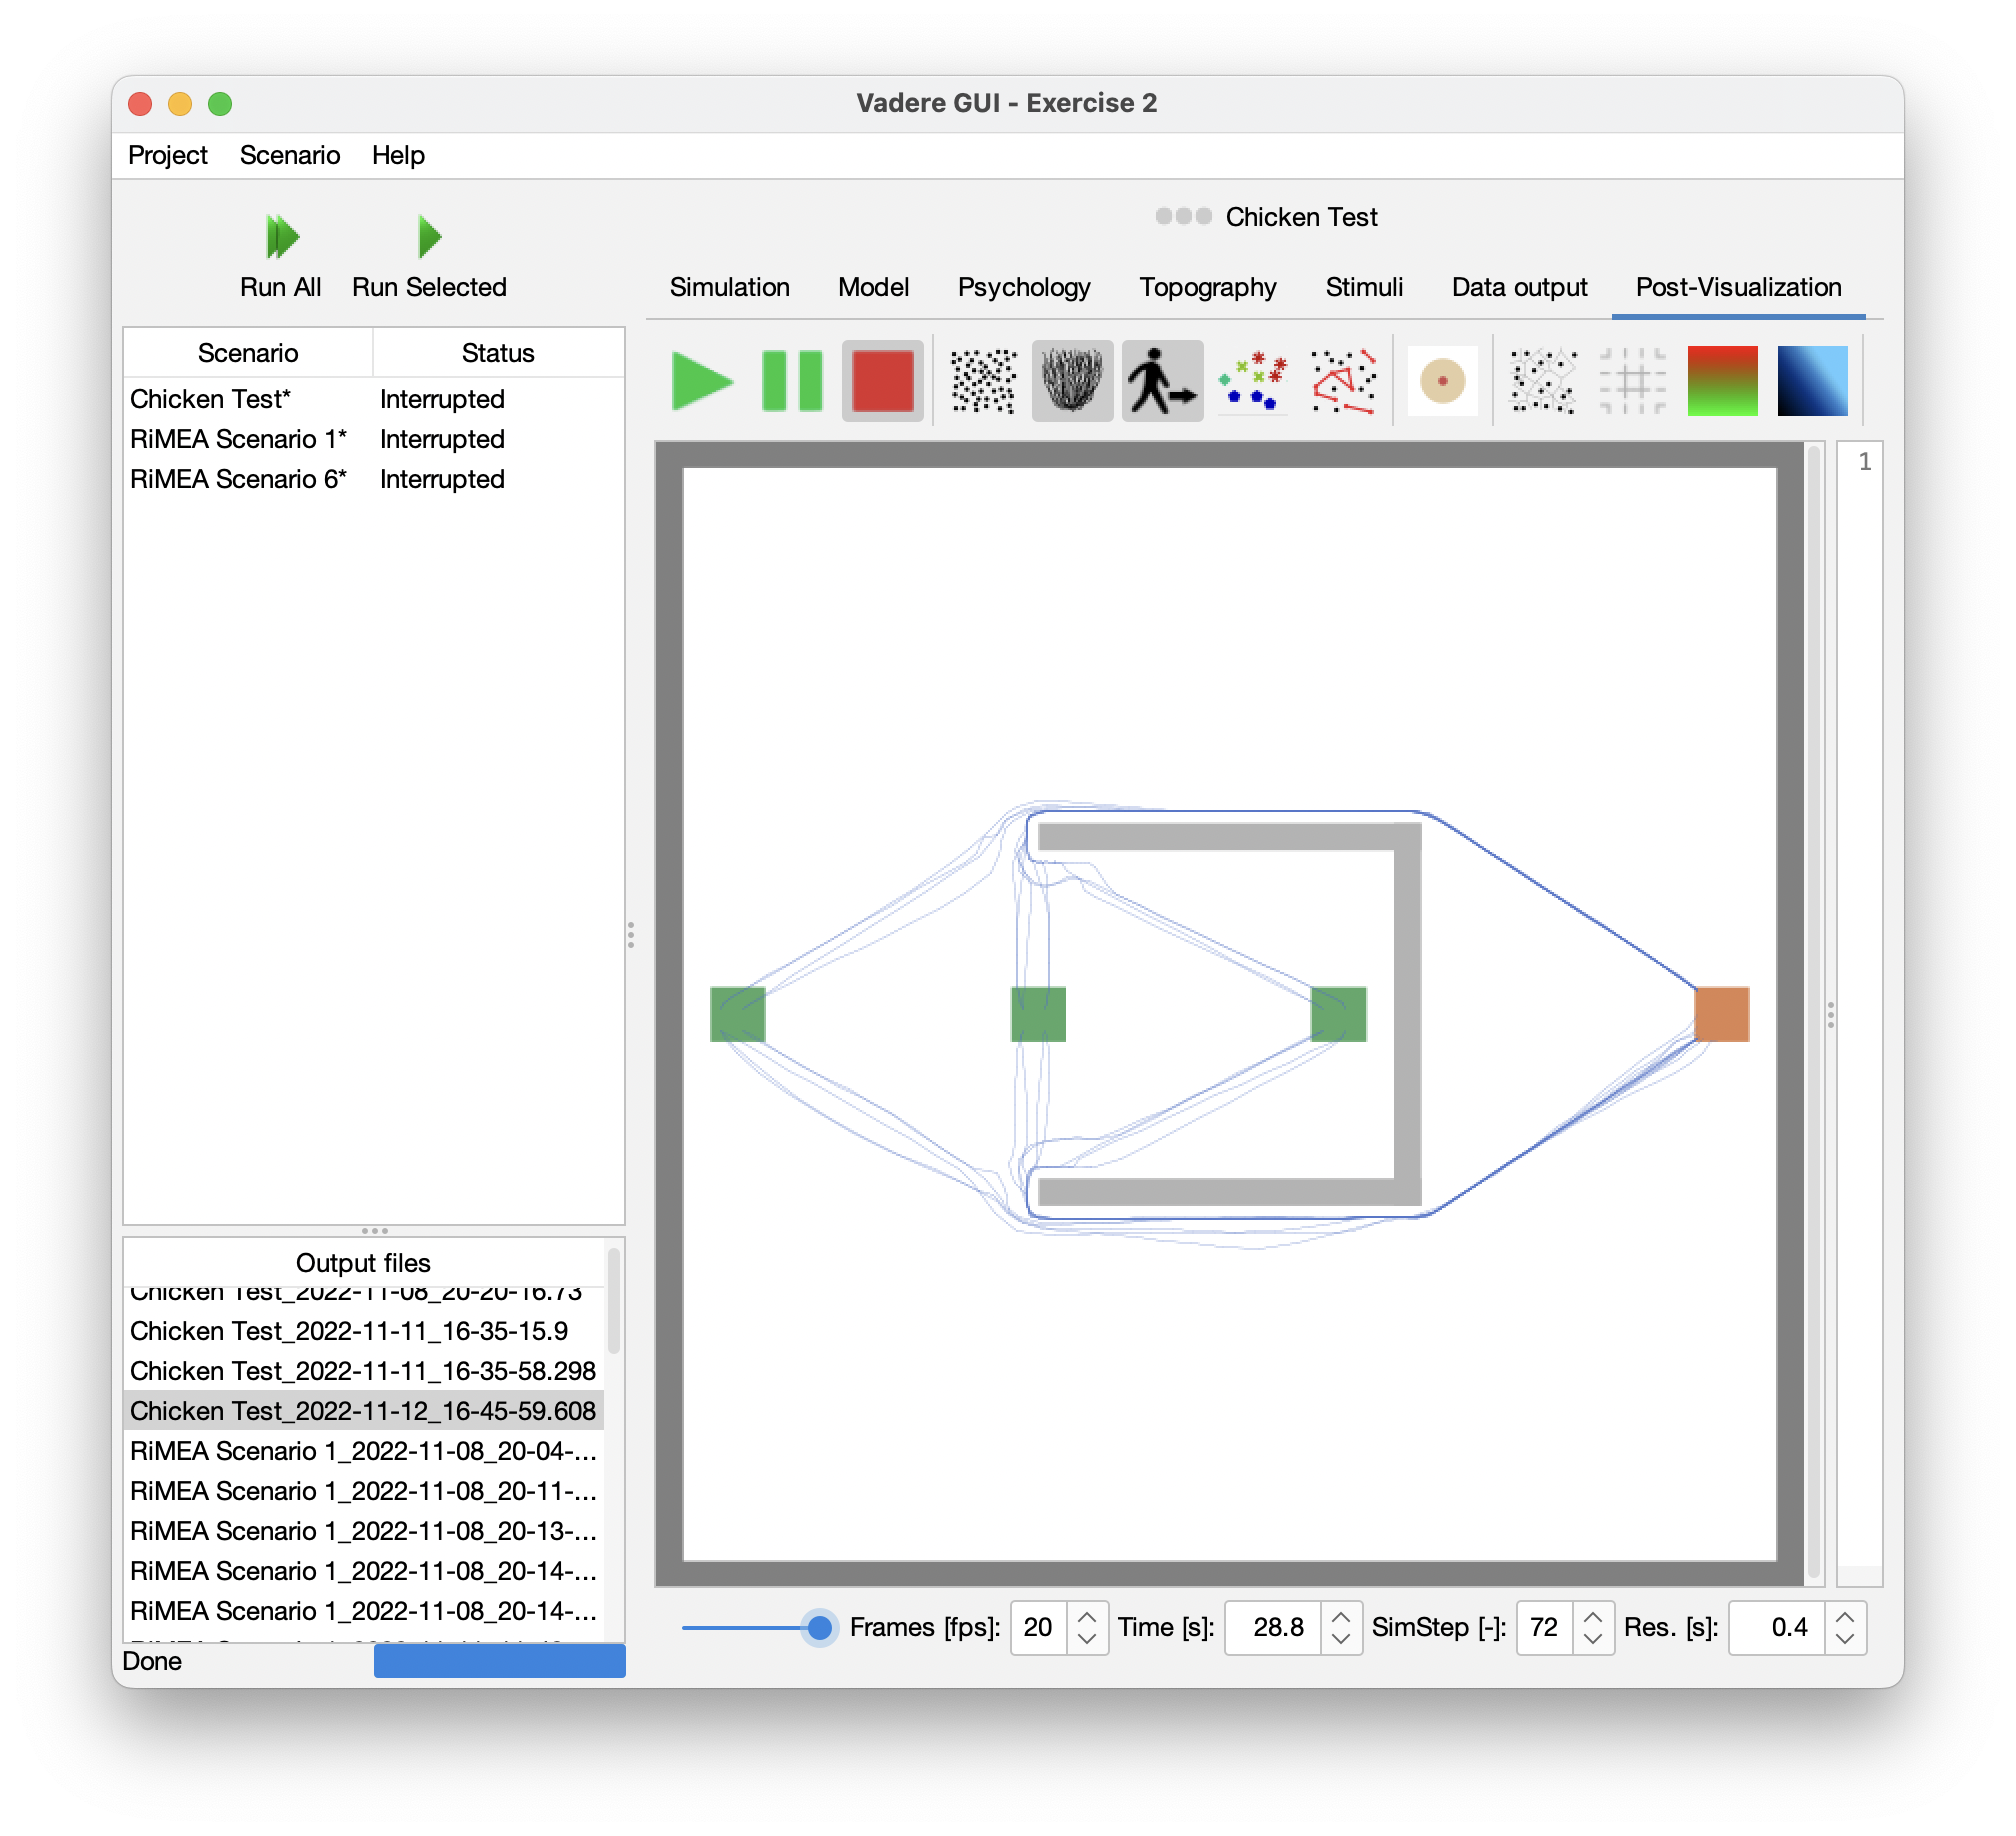
\includegraphics[width=0.33\textwidth]{images/gnm_chickenc.png}}
        \caption{Comparison of the chicken test between the 3 models}
        \label{comparison_chickentest}
    \end{figure}

\end{task}

\clearpage

\begin{task}{3, Using the console interface from Vadere}

\noindent{\textbf{Running Vadere from command line}}

The first job asked in this task is to run the corner scenario (Scenario 6) by calling Vadere from the command line. The command used to run it is the following:
\begin{itemize}
  \item[] java -jar vadere-console.jar scenario-run
  \item[] --scenario-file ``/path/to/the/file/scenariofilename.scenario"
  \item[] --output-dir=``/path/to/output/folders"
\end{itemize}

The output files produced by running the scenario from the console were the same as the ones produced by running it in the graphical user interface. This has been checked by using the command \textit{diff} with the corresponding files to compare as inputs (Figure \ref{diff}).

\begin{figure} [H]
    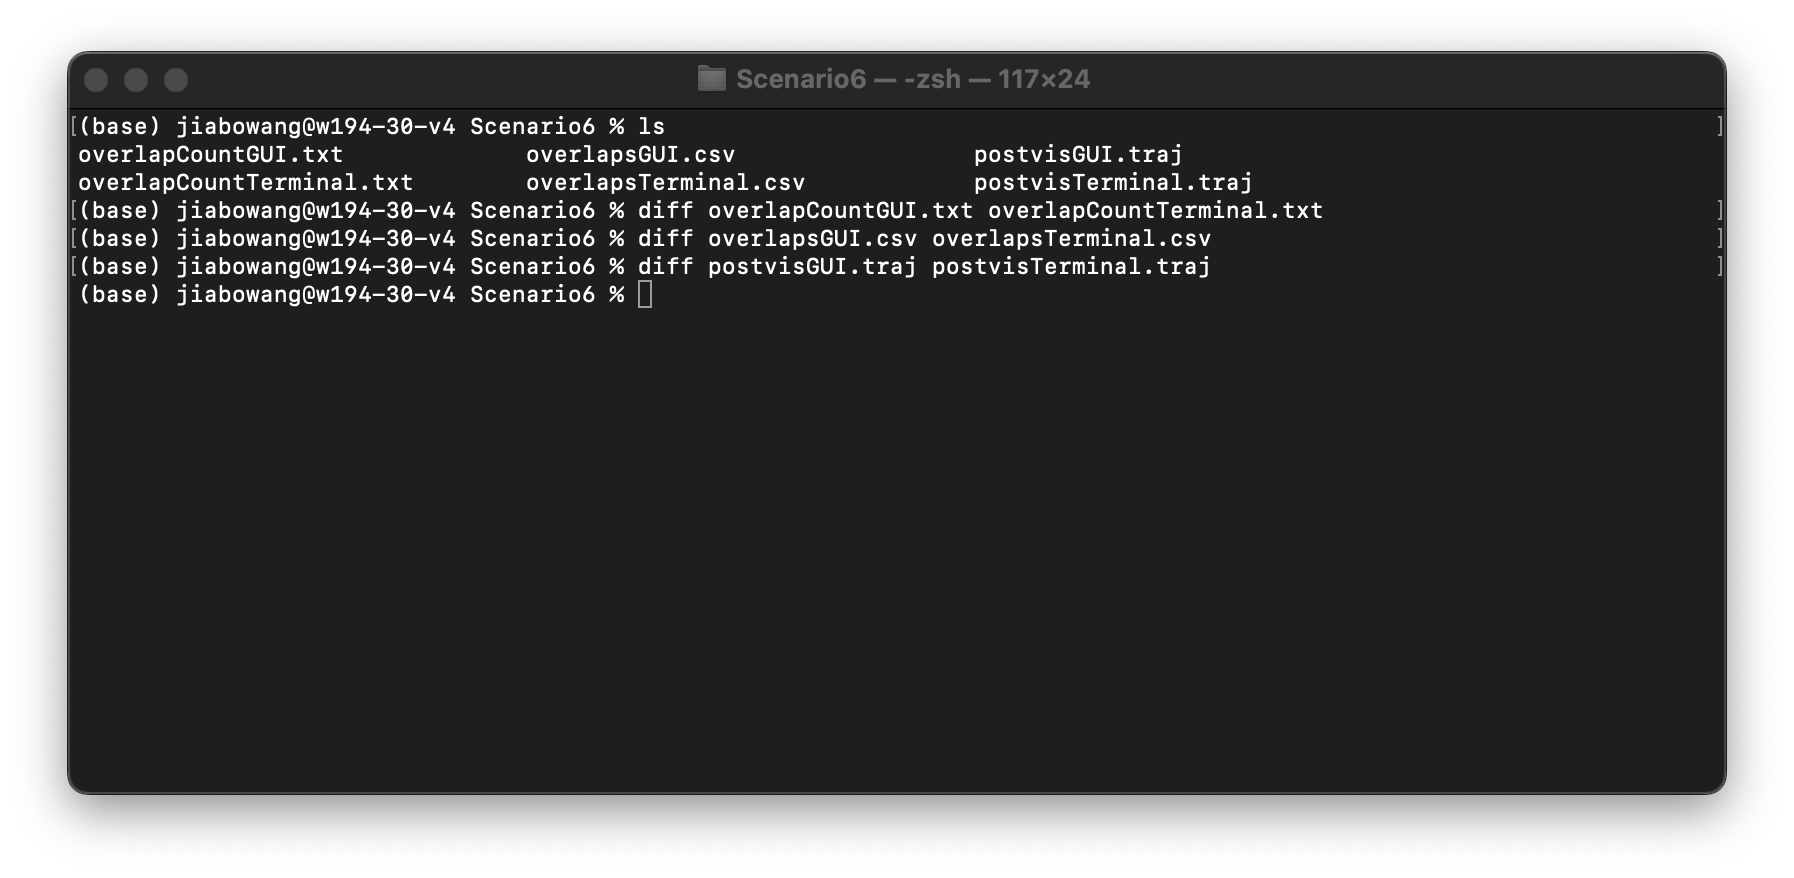
\includegraphics[width=10cm]{images/diff.png}
    \centering
    \caption{Command line of making diff with the output files}
    \label{diff}
\end{figure}

\noindent{\textbf{Adding pedestrians programmatically}}

Knowing that the scenario file represents a JSON file, in order to add pedestrians programmatically, the script \textit{add\_pedestrian.py} has been implemented. This script reads the scenario file, modifies the data by adding a pedestrian and saves it in JSON format. It has the following methods:
\begin{itemize}
  \item \textbf{read\_scenario(path)}: this method receives as a parameter the path where the scenario file is saved. The scenario is a JSON file, where the data is stored in a dictionary. The function of this method is to open the file, read it and return the data stored in a dictionary.
  \item \textbf{add\_pedestrian(data)}: this is the main method of the script. It takes as a parameter the data containing the information of the scenario and all it has to do is to add a pedestrian with all its attributes in the position (11.5, 1.5) as shown in the Figure \ref{sc_6_task_3} of the scenario and return the data. 
  \item \textbf{save\_scenario(path, data)}: finally, this method saves the modified data in the path of the parameter. 
\end{itemize}

Both input path and output path of the scenarios files are hard-coded and takes the ``corner scenario" (scenario 6) as demanded in the statement.

After executing this newly modified scenario file using both the console and the GUI, a comparison between the respective outputs has been done as in the previous section, and no differences have been observed. 

The added pedestrian is located nearer to the target than the ones from the source, for this reason, it takes him shorter to reach the target (12.8 s). The fastest one from the source needs 14.4 s and the last one reaches after 29.76 s. 


  \begin{figure} [H]
    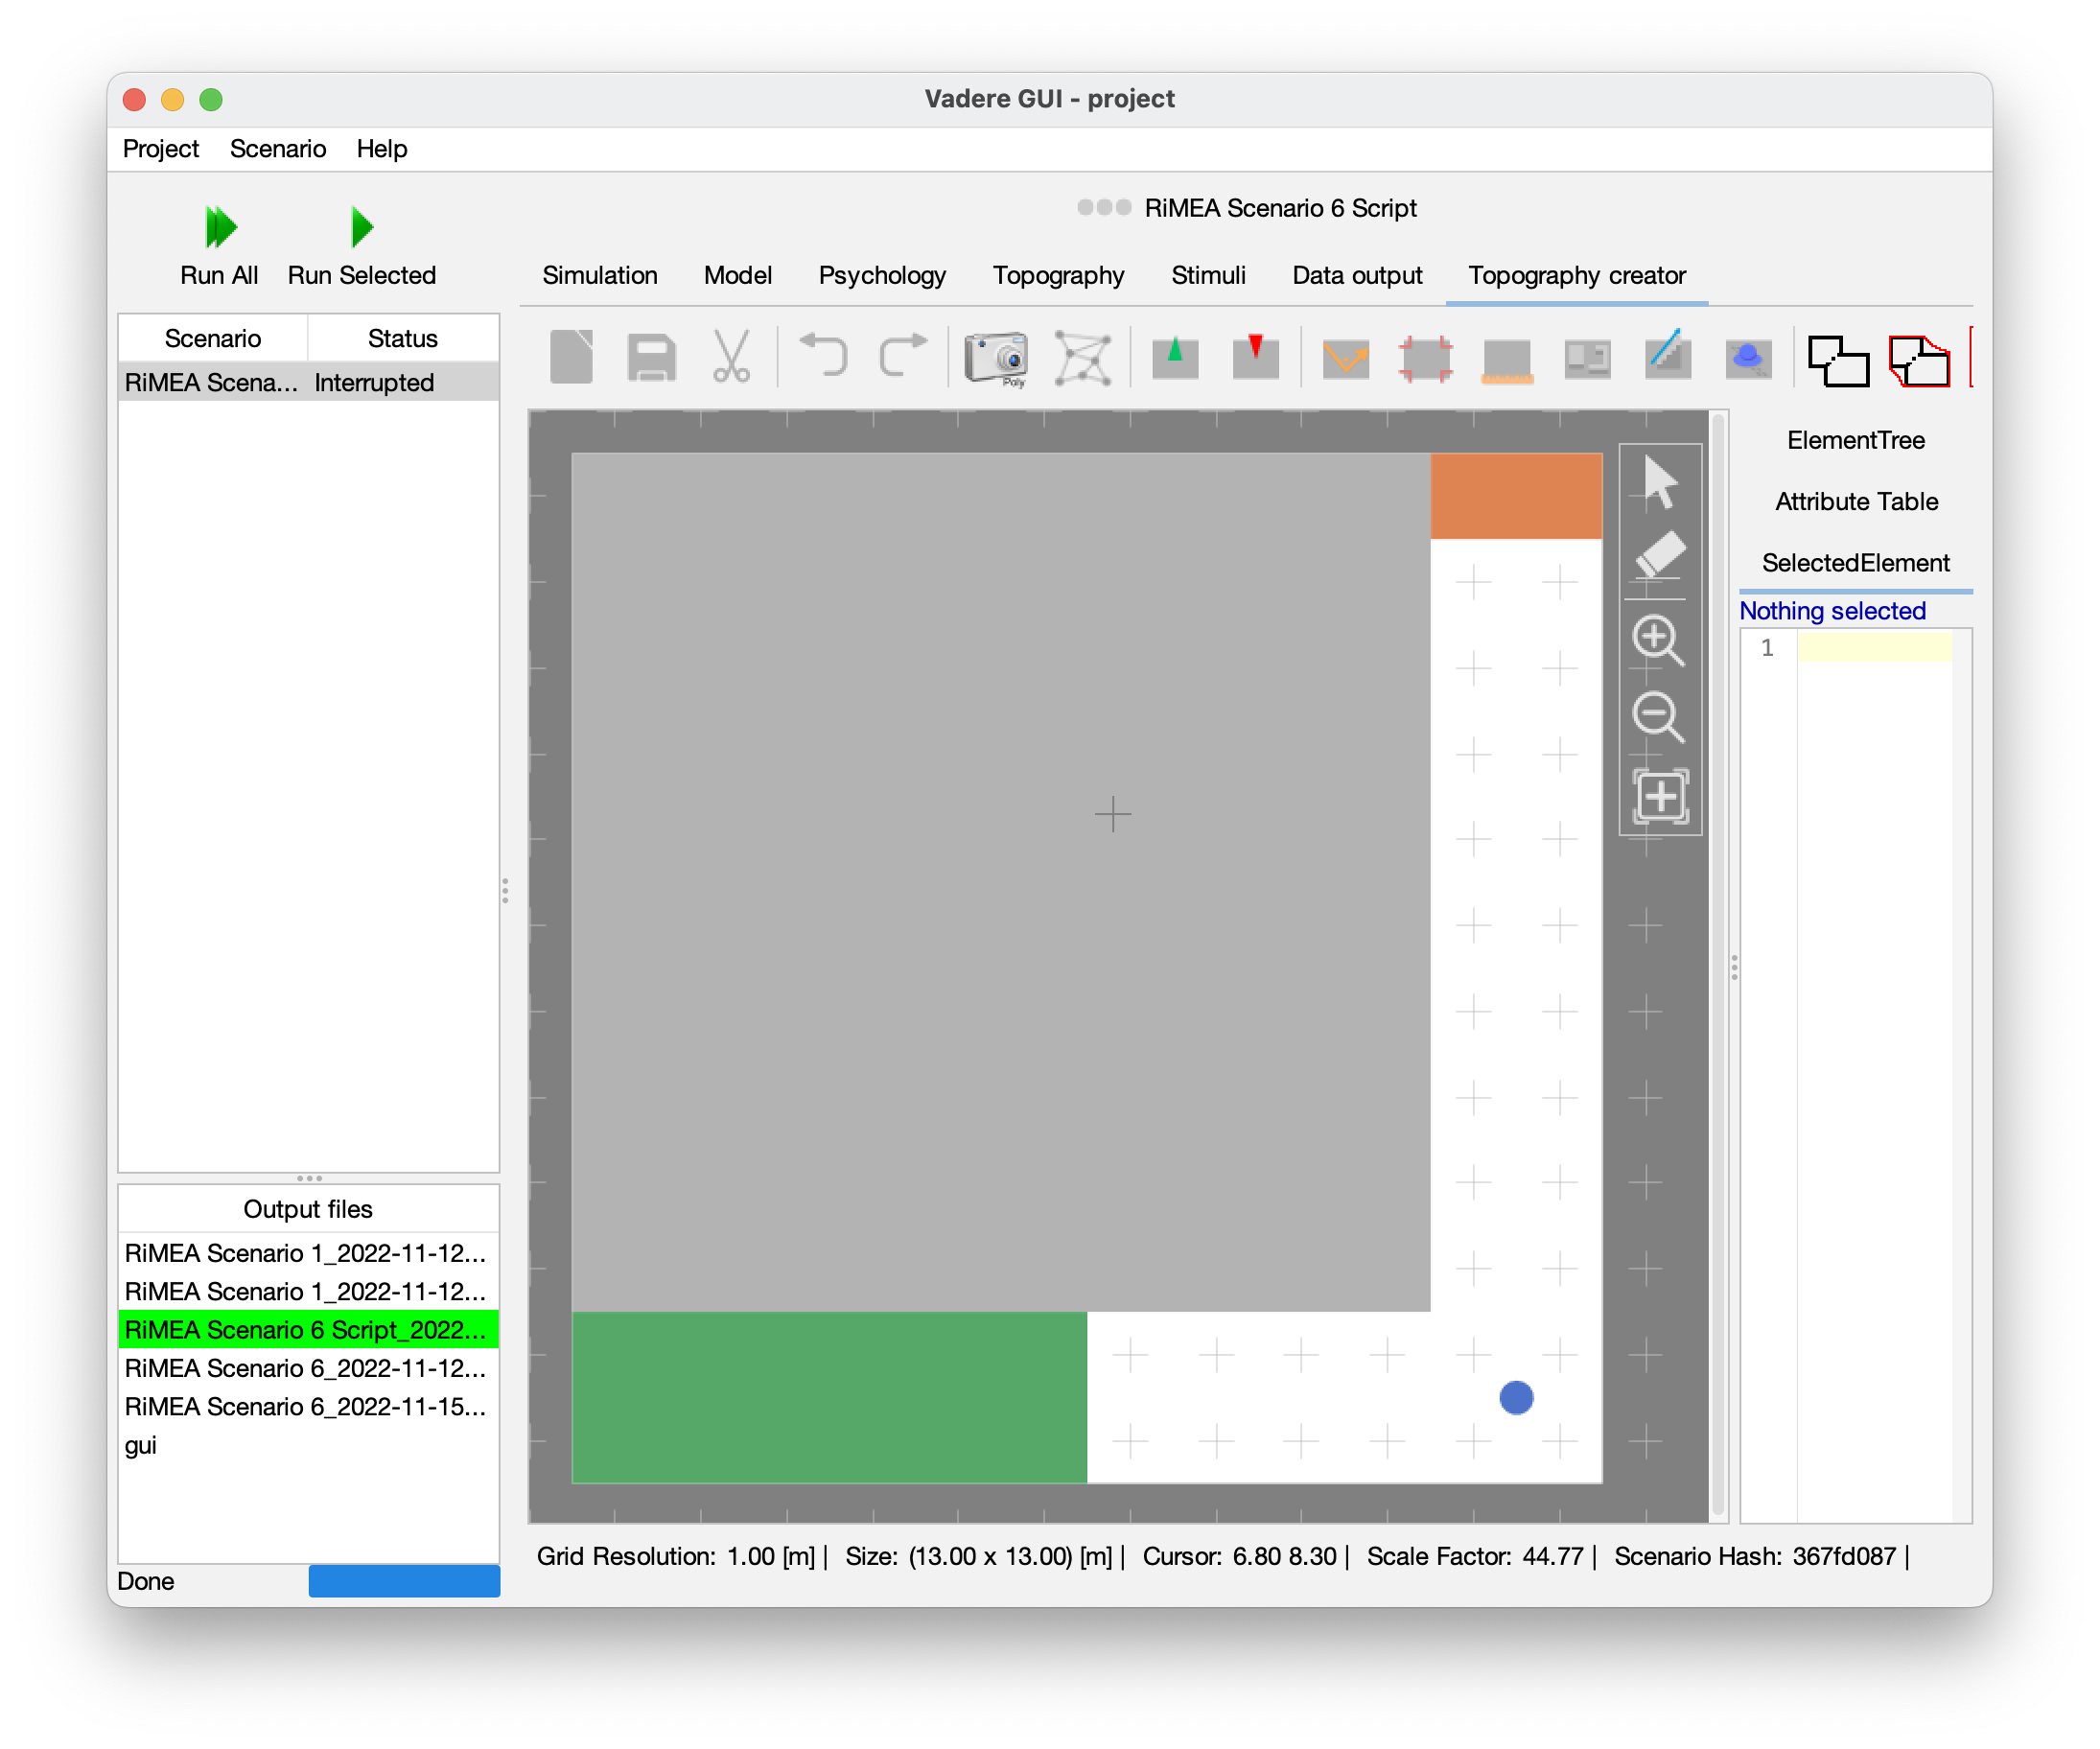
\includegraphics[width=10cm]{images/scenario6_task3.png}
    \centering
    \caption{Scenario 6 with a new added pedestrian in the corner}
    \label{sc_6_task_3}
  \end{figure}



\end{task}

\newpage

\begin{task}{4, Integrating a new model}

\noindent{\textbf{Integration of the SIR Model into Vadere}}

The integration of SIR model into Vadere at the beginning can be achieved by placing and replacing all the provided file within SIRGroupModel.zip into the appropriate package folders as the belonging location being indicated by the first line of each file. 

\begin{itemize}
    \item The files SIRGroup.java, SIRGroupModel.java and SIRType.java within folder ``sir" should be moved into a newly created folder at the directory VadereSimulator/src/org/vadere/simulator/models/groups/sir;
    \item AbstractGroupModel.java moved into VadereSimulator/src/org/vadere/simulator/models/groups;
    \item AttributesSIRG.java moved into VadereState/src/org/vadere/state/attributes/models;
    \item FootStepGroupIDProcessor.java moved into VadereSimulator/src/org/vadere/simulator/projects/ dataprocessing/processor.
\end{itemize}


\begin{figure} [H]
    \includesvg[width=15cm]{images/structure_UML.svg}
    \centering
    \caption{A concise UML class diagram showing the structure of SIR model and related classes}
    \label{diff}
\end{figure}

A more detailed explanation of each class follows below:

\begin{itemize}
\item[--] SIRGroup: this class represents a list of pedestrians which can be identified with an id.

\item[--] SIRGroupModel: this class extends the AbstractGroupModel class and defines the behaviour of a set of SIR groups (which are susceptible or infected in the first instance). It manages the infection process through the method \textit{update()}, which consists in iterating through all pedestrians in the simulation and, for each infected neighbor pedestrian within the specified infection distance, a draw is made and if the pedestrian is unlucky enough, it will get infected. Infected pedestrians are moved from the susceptible to the infected SIR group as a consequence.

\item[--] SIRType: this enummeration class represents the possible states of a pedestrian in a SIR Model: infected, susceptible or removed.

\item[--] AbstractGroupModel: this abstract class implements the \textbf{GroupModel} class.
    \begin{itemize}
        \item \textbf{registerMember(Pedestrian ped, T currentGroup)}: function to register the Pedestrian ped to the T currentGroup, it does not check whether the pedestrian is already a member of another group, so the caller has to make sure of that.
        \item \textbf{getNewGroup(int size)}: function to get a new group just by specifying the size of that group.
        \item \textbf{getNewGroup(final int id, final int size)}: function to get a new group with the id and the size specified by the parameters.
        \item \textbf{assignToGroup(Pedestrian pedestrian)}: function to assign a the Pedestrian pedestrian to a group.
    \end{itemize}

\item[--] AttributesSIRG: this class represents the different parameters of the infection behavior. 
    \begin{itemize}
        \item \textit{infectionsAtStart}: the initial number of pedestrian infected.
        \item \textit{infectionRate}: the probability such as one pedestrian can become infected if he/she is in contact with an infected pedestrian.
        \item \textit{infectionsMaxDistance}: the maximum range where a pedestrian can become infected if an infected pedestrian is located inside this range.
    \end{itemize}
    The three methods that this class have are the getters of the parameters described before. 

\item[--] FootStepGroupIDProcessor: data output processor to maintain the SIR information, that is the infection status. It is important to store this information for a post simulation analysis of the results.
    \begin{itemize}
        \item \textbf{doUpdate(SimulationState state)}: for each foot step of the trajectory it stores a new output composed of the current time, the pedestrian ID and its group ID.
    \end{itemize}

\end{itemize}

\noindent{\textbf{Analysis of the simulations}}

In order to be able to analyze the simulations, a new processor (FootStepGroupIDProcessor) has been added. Also a new file, SIRinformation.csv, has been added to the output. This file is linked with the FootStepGrouIDProcessor and contains the group information about the SIR model. As explained before in the class FootStepGroupIDProcessor, the data stored is composed by the pedestrian ID, its group ID and the simulation time of that moment. 

\bigskip

\noindent{\textbf{Correction of the SIR groups colors}}

The S, I, R groups are not visualized correctly in the current setup and a good and quick visualization of the different groups of the simulation is fundamental when we have to explain and analyze the behavior of them. So, changes have been done in the class SimulationModel.java in order to set the correct colors and be able to corretly visualize these colors. We have defined the following colors:
    \begin{itemize}
        \item \textbf{Infected pedestrian}: red (255, 0, 0) RGB color
        \item \textbf{Recovered pedestrian}: green (0, 255, 0) RGB color
        \item \textbf{Susceptible pedestrian}: blue (0, 0, 255) RGB color
    \end{itemize}

Firstly, in the class SimulationModel (Listing \ref{color_attributes}) we have added as attributes the colors mentioned before.
\begin{lstlisting}[language = Java, caption = new attributes of the SimulationModel class, label={color_attributes}]
protected final Color infected_color = new Color(255, 0, 0); 
protected final Color recovered_color = new Color(0, 255, 0);
protected final Color susceptible_color = new Color(0, 0, 255);
\end{lstlisting}

And then, in the constructor class of the class, we have the default coloring agent and finally adding the colors to the mapping (colorMap) between the group ID and the group coloring as we can see in the Listing \ref{SimulationModel}.
\begin{lstlisting}[language = Java, caption = constructor of the SimulationModel class, label={SimulationModel}]
public SimulationModel(final T config) {
	super(config);
	this.config = config;
	this.config.setAgentColoring(AgentColoring.GROUP); //added: to visualize corretly the group colors
	this.colorMap = new ConcurrentHashMap<>();
	this.colorMap.put(-1, config.getPedestrianDefaultColor());
	this.colorMap.put(0, infected_color);      //added: color
	this.colorMap.put(1, susceptible_color);   //added: color
	this.colorMap.put(2, recovered_color);     //added: color
	this.random = new Random();
}
\end{lstlisting}

Finally, remark that all the changes done before just enables to visualize the groups during simulation, the visualization does not work in the post visualization.

\bigskip

\noindent{\textbf{Efficiency improvement of the infection process}}

As said before, the infection process is managed through the method \textit{update()} of the class \textit{SIRGroupModel}. This method consists in a double for loop: all pedestrians checking for all pedestrians to determine if there are any infected neighbors within the infection radius,  which is very inefficient. To make it even worse, all the work done for iterating through the neighbors of a certain pedestrian can end up being useless, since that pedestrian could have already been infected and this condition is not checked until the very end of the inner loop.

As shown in Listing \ref{update_method}, two improvements have been made to this method: instead of checking if a pedestrian belongs to the susceptible group at the very end of the inner loop, check it before going through all its neighbors; and instead of looping through all pedestrians in the inner loop, only loop through those within the radius of infection. This second improvement takes advantage of the \textit{LinkedCellsGrid} class, concretely the \textit{getObjects()} method, which given a position and a radius, loops only through the cells within the given radius and returns a list of objects of the requested class, which is \textit{Pedestrian} in this case.

\begin{lstlisting}[language = Java, caption = Improved version of the infection process, label={update_method}]
public void update(final double simTimeInSec) {
	// Check the positions of all pedestrians and switch groups to INFECTED (or REMOVED).
	DynamicElementContainer<Pedestrian> c = topography.getPedestrianDynamicElements();
	LinkedCellsGrid<Pedestrian> grid = c.getCellsElements();
	double infectionRadius = attributesSIRG.getInfectionMaxDistance();
	double infectionRate = attributesSIRG.getInfectionRate();
	if (c.getElements().size() > 0) {
		for(Pedestrian p : c.getElements()) {
			// Only check for susceptible pedestrians, skip already infected ones
			SIRGroup g = getGroup(p);
			if (g.getID() == SIRType.ID_INFECTED.ordinal())
				continue;
			// Get neighbors within a radius of infectionRadius from the position of the Pedestrian p
			VPoint position = p.getPosition();
			List<Pedestrian> neighbors = grid.getObjects(position, infectionRadius);
			// Try to infect p with probability infectionRate with as many attempts as infected neighbors are there
			for (Pedestrian n : neighbors) {
				if (p == n || getGroup(n).getID() != SIRType.ID_INFECTED.ordinal())
					continue;
				if (this.random.nextDouble() < infectionRate) {
					elementRemoved(p);
					assignToGroup(p, SIRType.ID_INFECTED.ordinal());
				}
			}
		}
	}
}
\end{lstlisting}

\newpage

\noindent{\textbf{Testing and results}}

Once fixed all the problems mentioned before, now it is possible to run some scenarios with the modified Vadere software and analyze some results. In particular, we are going to analyze the behavior of the pedestrians in 2 different scenarios:
    \begin{itemize}
        \item \textbf{Scenario 1}: a fairly large static scenario of 50m x 50m with a source spawning 1000 pedestrians, and a target exactly over of the source, which is not absorbing. The 1000 pedestrians are randomly created, by setting spawnAtRandomPositions as true and useFreeSpaceOnly as false. Over the 1000 pedestrians, 10 are infective and 990 are susceptible. The objective of this test is to see how the susceptible and infective pedestrians change over time.
        \item \textbf{Scenario 2}: a dynamic corridor scenario of 40m x 20m, where one group of 100 susceptible pedestrians moves from left to right, and another group of 100 infected pedestrians moving from right to left. The pedestrians are created over time (not all at the same time) so the attribute useFreeSpaceOnly is set as true. The objective of this test is to see how many pedestrians get infected in this counter-flow.
    \end{itemize}

Let's first explain about the first scenario, where two experiments have been done:
    \begin{itemize}
        \item the first one with the following attributes: The infection rate has been set to 0.05 (``infectionRate": 0.05) with 10 infected pedestrians infected at the beginning (``infectionsAtStart": 10) and the maximum infection distance is set to 1.0 (``infectionMaxDistance": 1.0). The simulation will be executed with a simulation time ratio of 1.0 (``realTimeSimTimeRatio" = 1.0) and the time step will be 0.5 (``simTimeStepLength"= 0.5).
        After simulating this scenario, half of the population takes 26.1 s to become infected.

        \begin{figure} [H]
            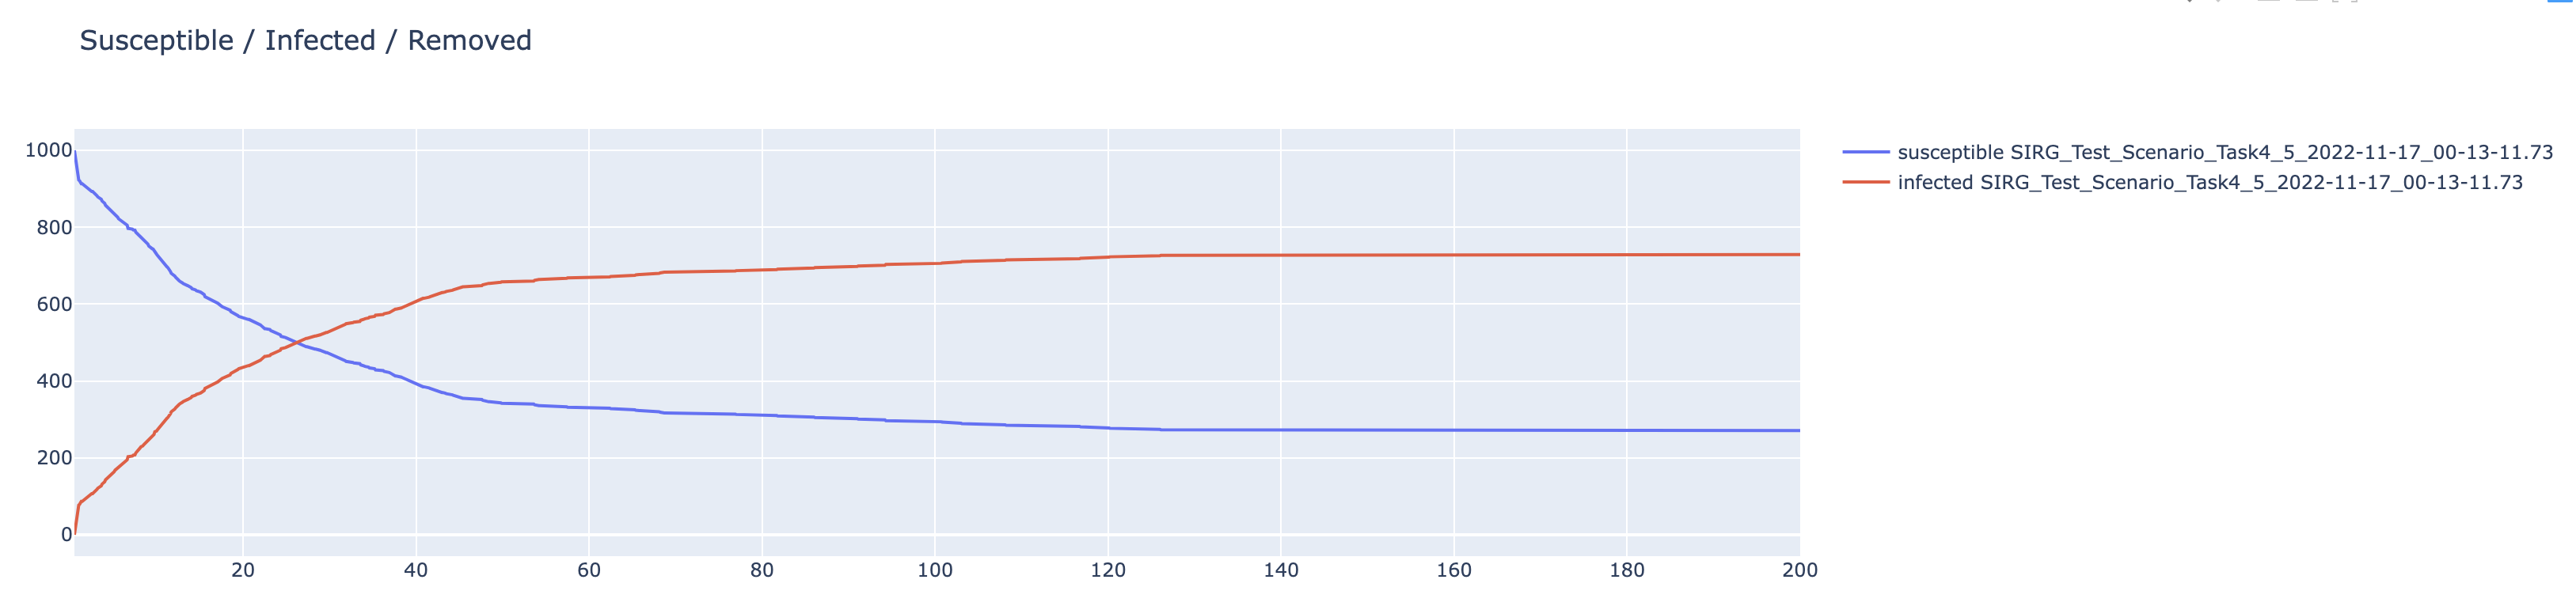
\includegraphics[width=15cm]{images/plot1.png}
            \centering
            \caption{Dash/Ploty view of a single simulation - time (x) and pedestrians (y)}
            \label{plot1}
        \end{figure}
        
        \item the second one with the same attributes as the first one, with the only difference that the infection rate is increased to 0.1. 
        As expected, after increasing the infection rate, the infection is spreading faster and in fact, half of the population become infected in a shorter time, just 5.7 s.

        \begin{figure} [H]
            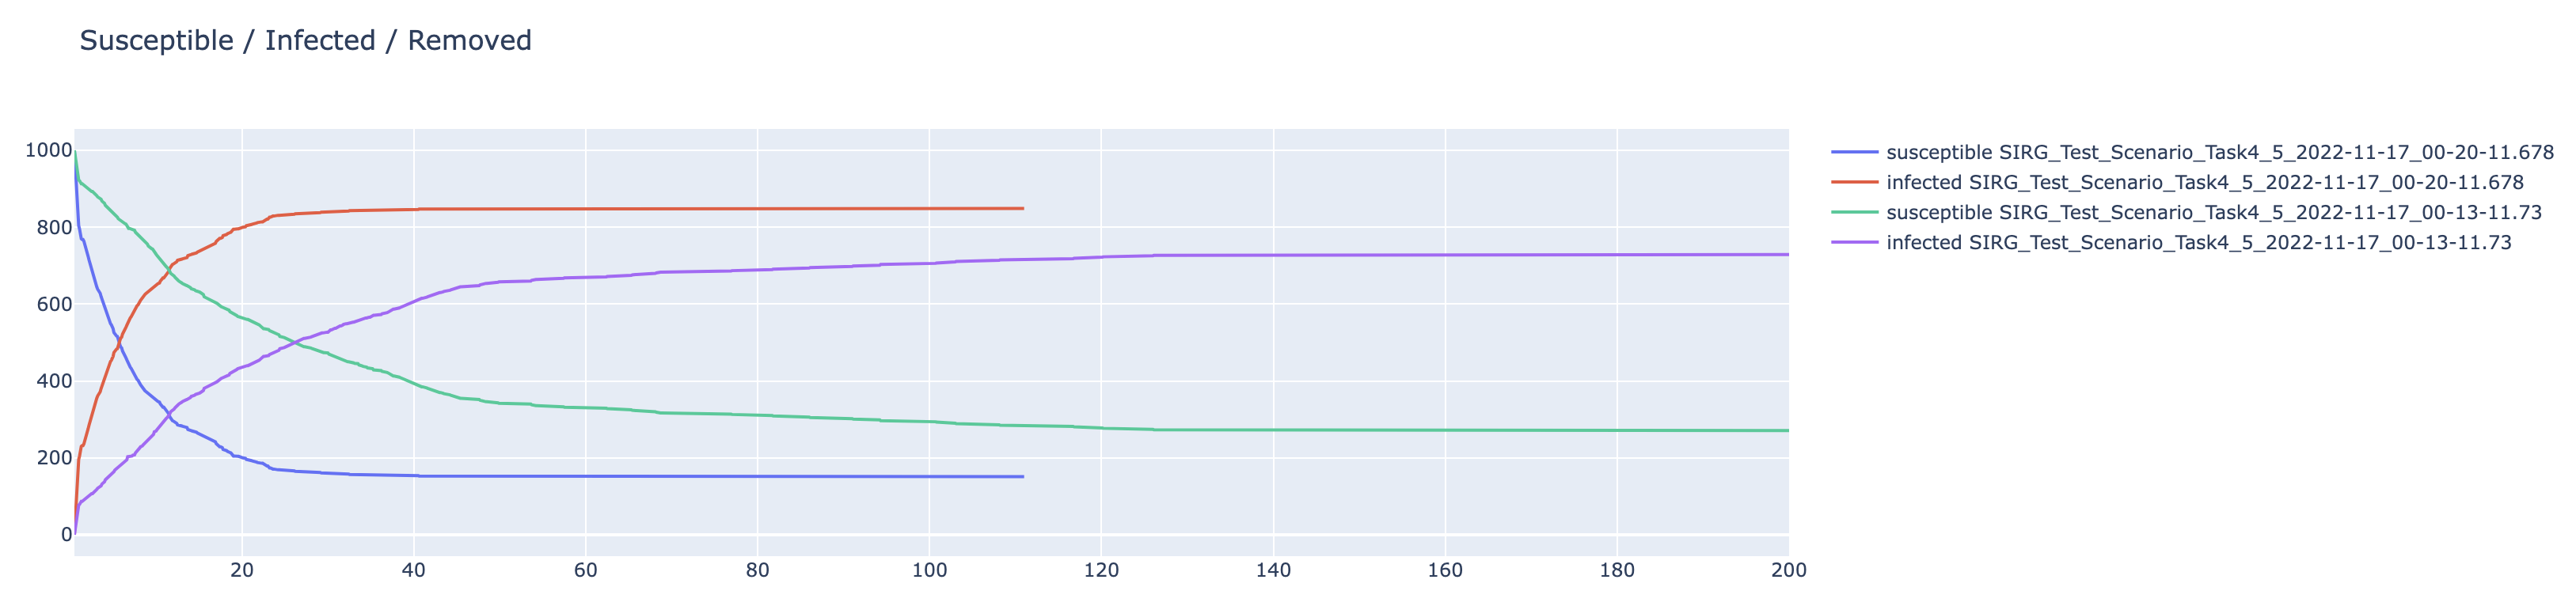
\includegraphics[width=15cm]{images/plot2.png}
            \centering
            \caption{Dash/Ploty view of the multiple simulation - time (x) and pedestrians (y)}
            \label{plot2}
        \end{figure}
        
    \end{itemize}

As shown in the Figures \ref{plot1} and \ref{plot2} of the Dash/Ploty views, a better graphically of how the infection is spreading can be seen. Obviously, the scenario with 0.1 infection rate delivers a faster infection spreading and becomes establish much quicker than the scenario with a smaller infection rate.
Finally, in the figure \ref{task4} we can see an example of the simulation of the first scenario in the GUI.

\begin{figure} [H]
    \centering
    \subfloat[At the beginning of the simulation]{
        \label{t_4a}
        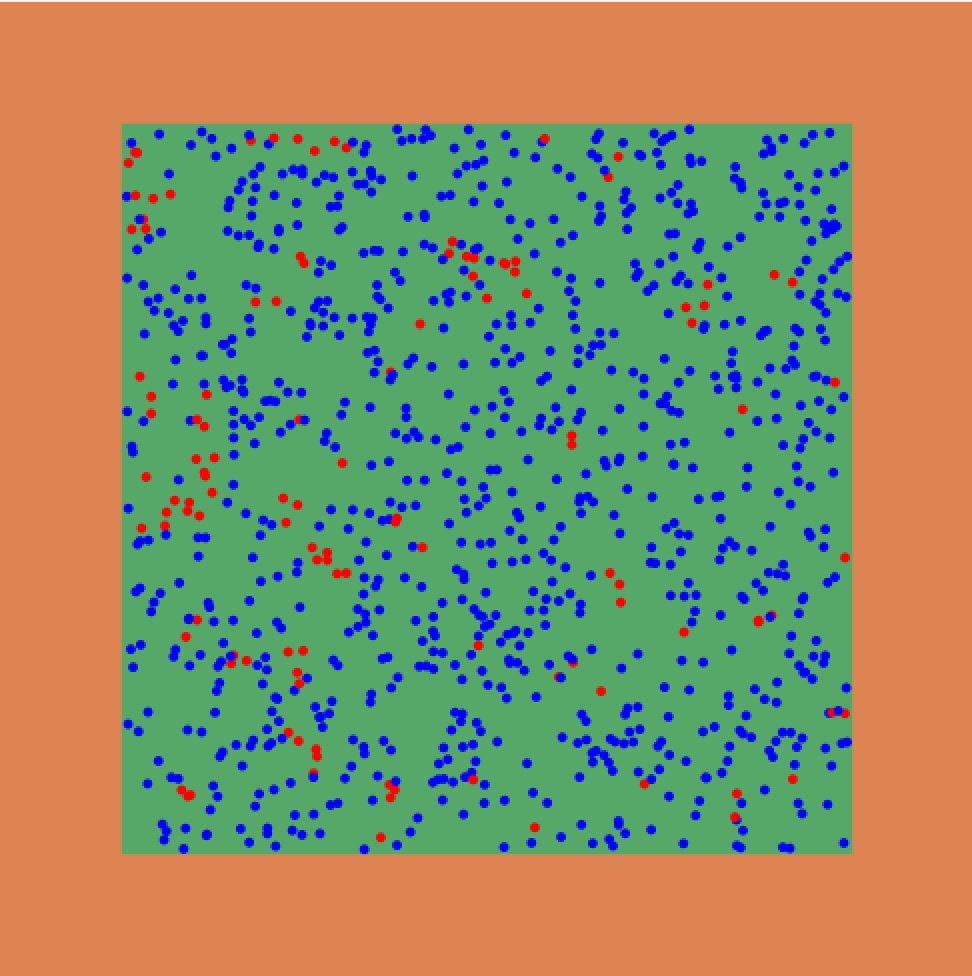
\includegraphics[width=0.33\textwidth]{images/task4_1.png}}
        \subfloat[In the middle of the simulation]{
        \label{t_4b}
        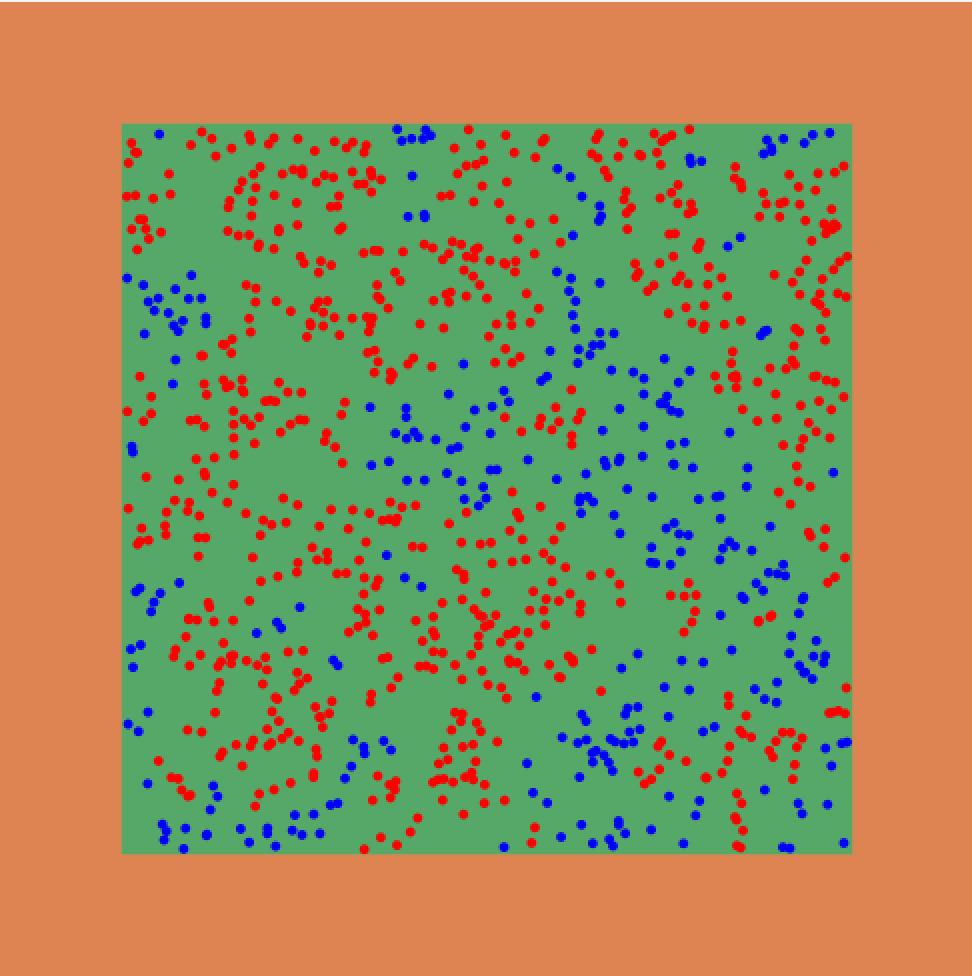
\includegraphics[width=0.33\textwidth]{images/task4_2.png}}
        \subfloat[At the end of the simulation]{
        \label{t_4c}
        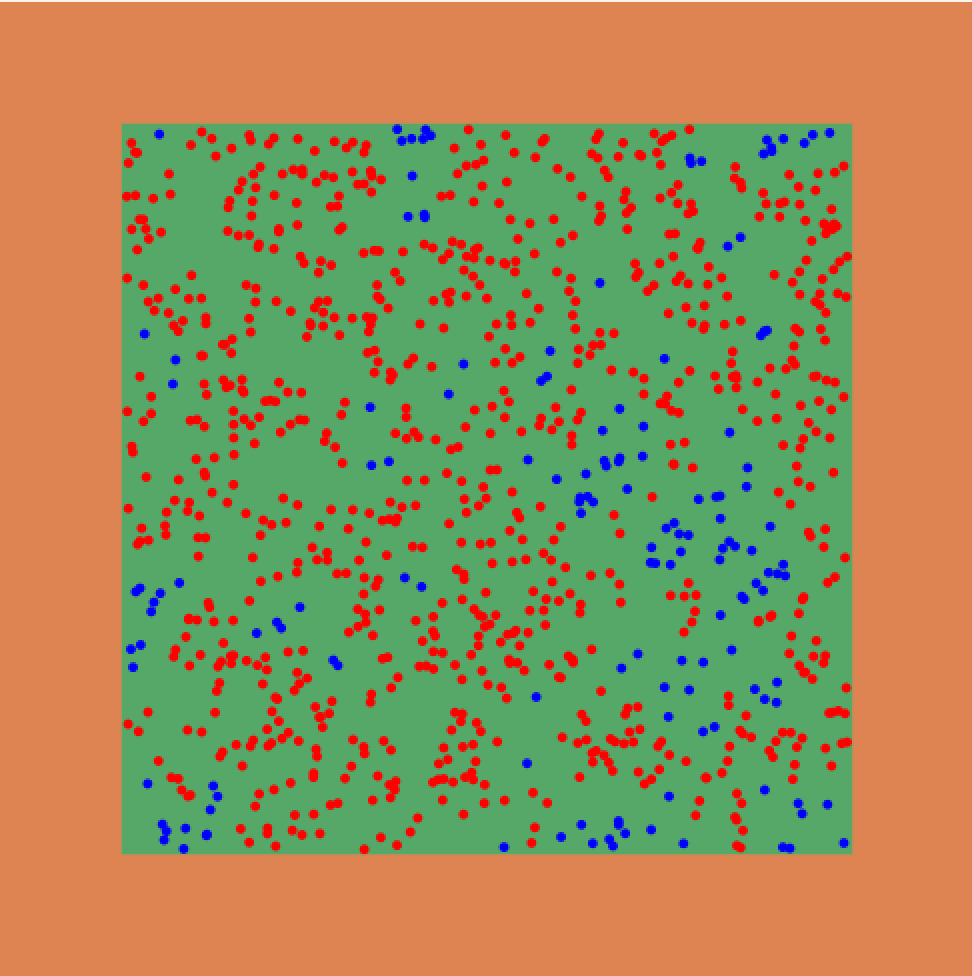
\includegraphics[width=0.33\textwidth]{images/task4_3.png}}
        \caption{Different stages of the simulation of the first scenario}
        \label{task4}
\end{figure}

Regarding the second scenario, a dynamic corridor scenario of 40m x 20m with the following parameters: the infection rate has been set to 0.05 (``infectionRate": 0.05) with 10 infected pedestrians infected at the beginning (``infectionsAtStart": 10) and the maximum infection distance is set to 1.0 (``infectionMaxDistance": 1.0). The simulation will be executed with a simulation time ratio of 1.0 (``realTimeSimTimeRatio" = 1.0) and the time step will be 0.5 (``simTimeStepLength"= 0.5). And the attribute useFreeSpaceOnly as true.

In this case, to make it more realistic, there are infected pedestrians in both groups. Because it is not realistic to have just infected pedestrians in one side and susceptible pedestrians on the other side.

An example of the simulation of this scenario is shown in the following figure \ref{task4_2}

\begin{figure} [H]
    \centering
    \subfloat[At the beginning of the simulation]{
        \label{t_4d}
        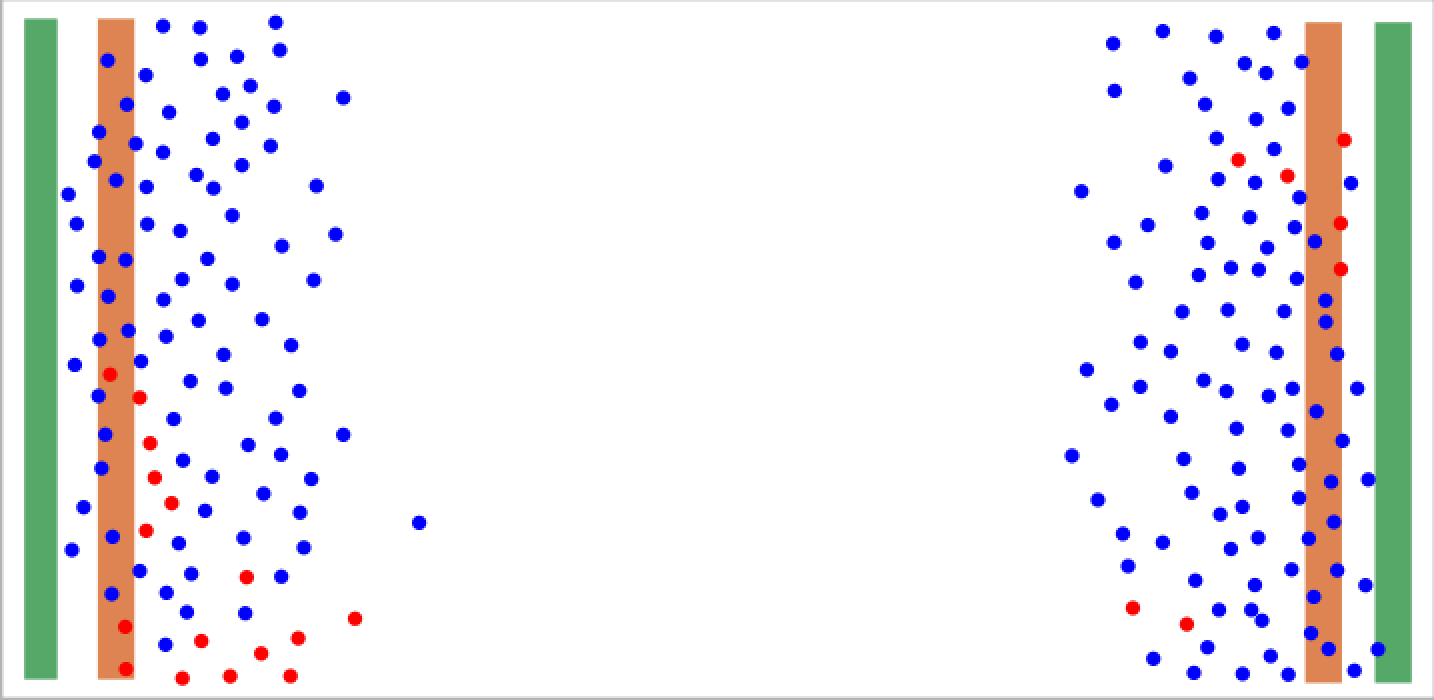
\includegraphics[width=0.33\textwidth]{images/task4_4.png}}
        \subfloat[In the middle of the simulation]{
        \label{t_4e}
        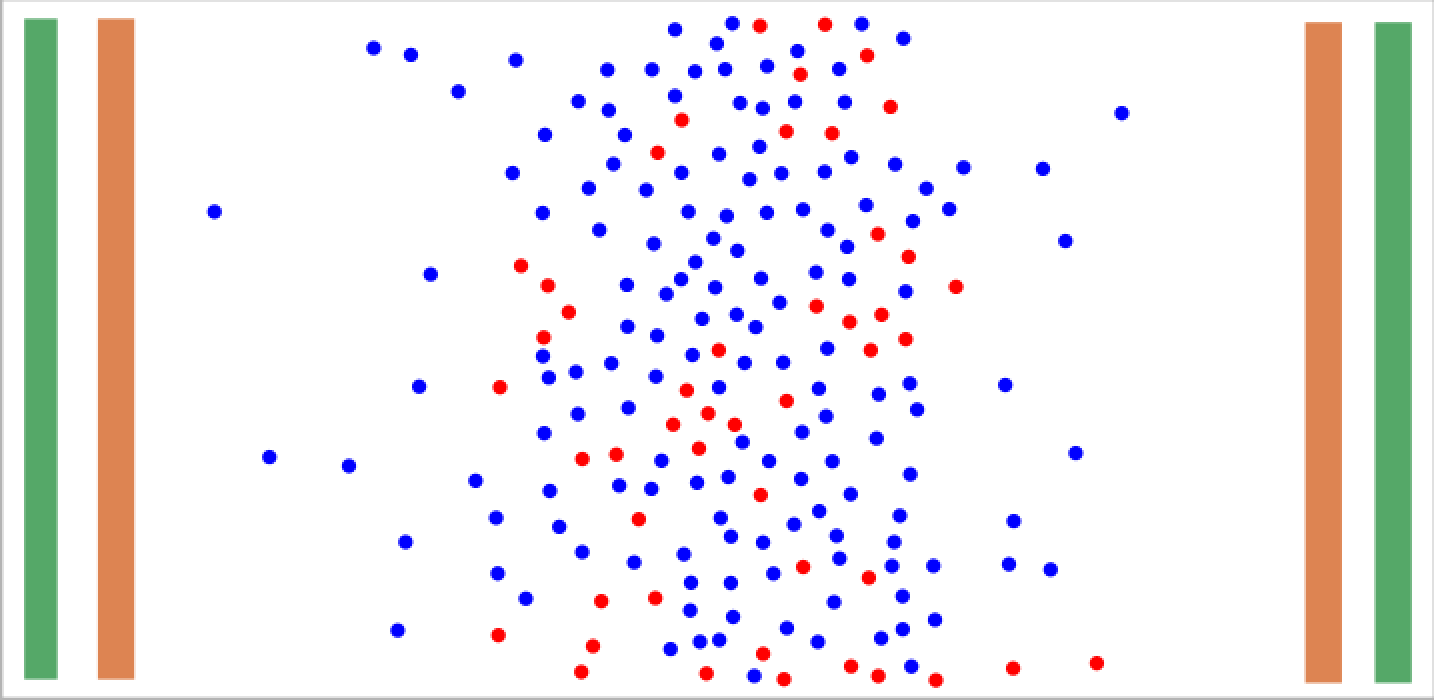
\includegraphics[width=0.33\textwidth]{images/task4_5.png}}
        \subfloat[At the end of the simulation]{
        \label{t_4f}
        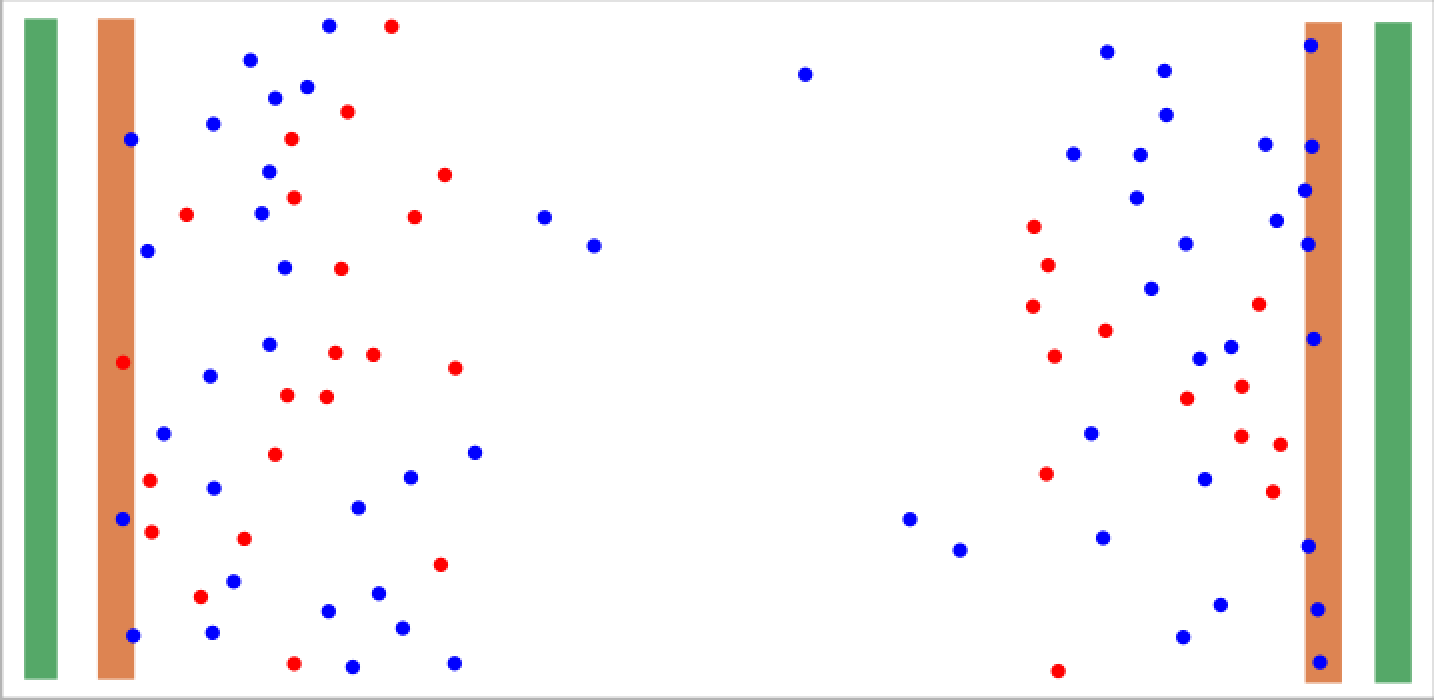
\includegraphics[width=0.33\textwidth]{images/task4_6.png}}
        \caption{Different stages of the simulation of the second scenario}
        \label{task4_2}
\end{figure}

As expected, in the middle of the simulation (Figure \ref{t_4e}), the number of the infected pedestrians have increased because there is a counter-flow between non-infected and infected pedestrians of the two groups. And at the end of the simulation (Figure \ref{t_4f}) it can be observed that the number of infected pedestrians are much more than at the beginning of the simulation.  

\begin{figure} [H]
    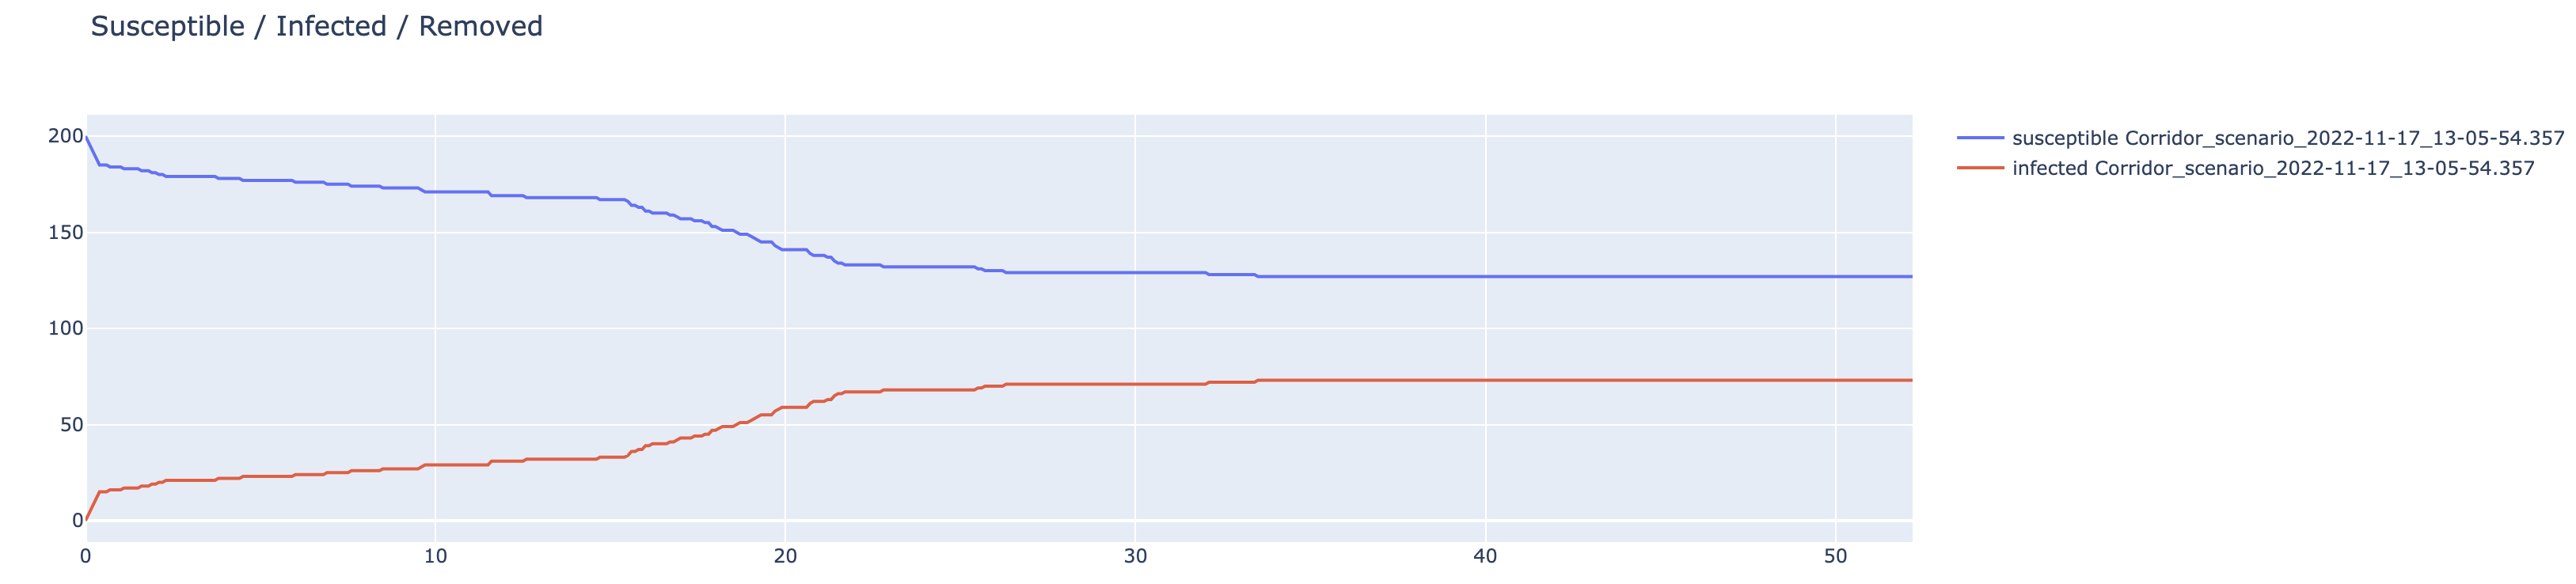
\includegraphics[width=15cm]{images/plot3.png}
    \centering
    \caption{Dash/Ploty view of the scenario 2 simulation - time (x) and pedestrians (y) with 10 infected pedestrians at start}
    \label{plot3}
\end{figure}

\newpage

In the Figure \ref{plot3} we can see a better evolution of the number of infected and susceptible pedestrians during the simulation. The interaction of the two groups can be identified during the periods of 15.5s and 22.5s, where the number of infected pedestrians increases from 34 to 67, so 23 healthy pedestrians become infected during the counter-flow. After the counter-flow, the number of susceptible and infected pedestrians is again stabilised. The number of infected pedestrians does not surpass the number of susceptible pedestrians because the initial number of infected pedestrians is not very big (10), if we increase this parameter, for example to 50, a much bigger number of pedestrians become infected at the end as we can see in the next Figure \ref{plot4} and the number of infected pedestrians is increased much more during the counter-flow. The same effect can be achieved by increasing the infection rate.

\begin{figure} [H]
    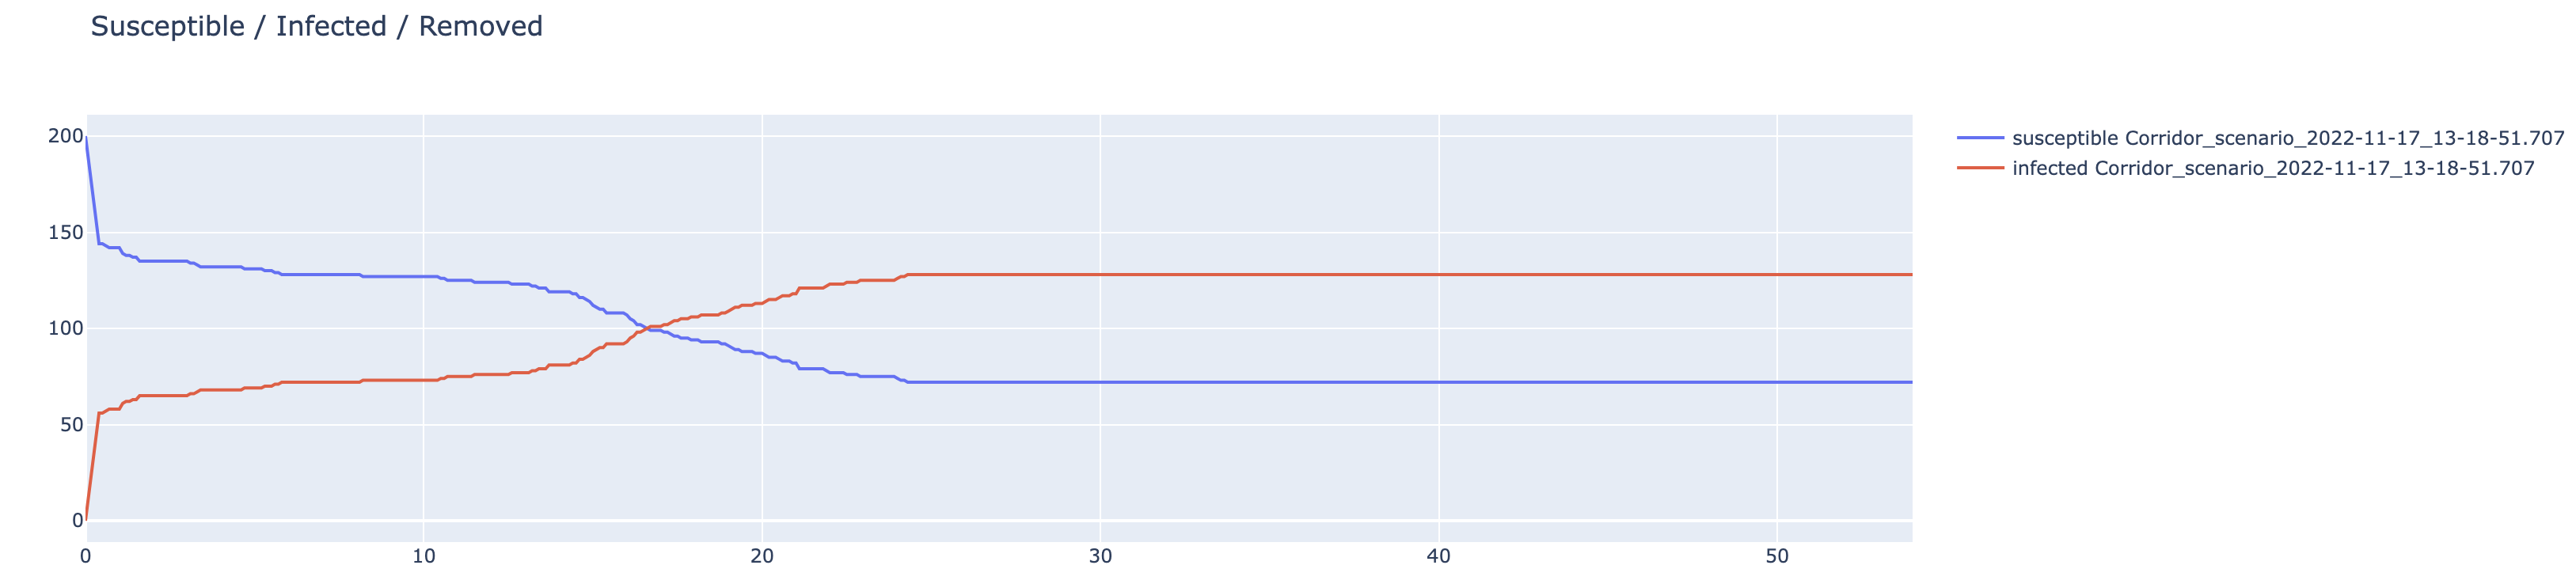
\includegraphics[width=15cm]{images/plot4.png}
    \centering
    \caption{Dash/Ploty view of the scenario 2 simulation - time (x) and pedestrians (y) with 50 infected pedestrians at start}
    \label{plot4}
\end{figure}

\noindent{\textbf{Infection rate and time step decoupling}}

A way to decouple the infection rate and the time step would be to fix the \textit{update()} method to execute once every certain time independently of the time step size.

This can be done by implementing an accumulator/repeater: for every invokation of \textit{updateLocomotionLayer()}, which is the method that calls \textit{update()}, instead of calling \textit{update()} every time, depending on whether the time step is greater or less than the fixed time, the \textit{update()} method may be called many times at once or once every a certain number of calls. This allows the fixed time to be as flexible as possible: for example, given a time step of size 0.5, if the fixed time is 2 seconds, the infection process should be executed once every four calls of \textit{updateLocomotionLayer()}; if the fixed time is 0.25 seconds, it should be executed twice every one call.

The implementation of this decoupling is shown in Listing \ref{decoupling}. A private attribute \textit{accumulatedTime} has been added for keeping track of the accumulated time. The while loop is enough for treating both cases. This should only affect the SIR model, therefore an if condition of the model being an instance of such class has been added.

\newpage

\begin{lstlisting}[language = Java, caption = Decoupled version of the \textit{updateLocomotionLayer()} method, label={decoupling}]
private double accumulatedTime = 0.0;

// ...

private void updateLocomotionLayer(double simTimeInSec) {
	for (Model m : models) {
		List<SourceController> stillSpawningSource = this.sourceControllers.stream().filter(s -> !s.isSourceFinished(simTimeInSec)).collect(Collectors.toList());
		int pedestriansInSimulation = this.simulationState.getTopography().getPedestrianDynamicElements().getElements().size();
		int aerosolCloudsInSimulation = this.simulationState.getTopography().getAerosolClouds().size();

		// Only update until there are pedestrians in the scenario or pedestrian to spawn or aerosol clouds persist
		if (!stillSpawningSource.isEmpty() || pedestriansInSimulation > 0 || aerosolCloudsInSimulation > 0) {
			if (m instanceof SIRGroupModel) {
				accumulatedTime += this.attributesSimulation.getSimTimeStepLength();
				// fixedTime can be any positive value
				double fixedTime = 1.0;
				while (accumulatedTime >= fixedTime) {
					m.update(simTimeInSec);
					accumulatedTime -= fixedTime;
				}
			}
			else m.update(simTimeInSec);

			if (topography.isRecomputeCells()) {
				// rebuild CellGrid if model does not manage the CellGrid state while updating
				topographyController.update(simTimeInSec); //rebuild CellGrid
			}
		}
	}
}
\end{lstlisting}

\noindent{\textbf{Possible extensions of the model beyond}}

It is broadly known (specially nowadays) that there are a lot of factors involved in the propagation, recovery and symptoms of a disease: indoor spaces might increase the infection ratio, pedestrians with healthy habits might take faster to recover from a disease or have less symptoms... Therefore, many features could be added as extensions of the model beyond and would help to make it more realistic and customizable, some examples are:

\begin{itemize}
    \item[--] Face masks and indoor spaces: a pedestrian might wear a face mask. Face masks could reduce the infection ratio. Pedestrians staying for too long in indoor spaces might constantly increase the infection ratio.
    \item[--] Vaccinated: a vaccinated pedestrian might recover faster from a disease than a non-vaccinated one. It could also reduce the ratio of being infected (or even dying). In addition, the effectiveness of a vaccine might change over time.
    \item[--] Age: the age of a pedestrian might affect the recovery period and even the death ratio. It would be different for every age group, depending on the characteristics of the disease. For example, kids might be less susceptible than elders. Elders might have a higher death ratio.
\end{itemize}

\end{task}

\clearpage

\begin{task}{5, Analysis and visualization of results}

\noindent{\textbf{Adding the recovered state}}

For the recovered state representing recovered pedestrians, which cannot get re-infected and cannot infect susceptible persons, since the removed state will not be considered in this exercise, it has been substituted for this new state. The overall changes are the following:
\begin{itemize}
    \item[--] \textit{ID\_RECOVERED} added to the enumeration class \textit{SIRType}.
    \item[--] \textit{recoveryRate} attribute added to the \textit{AttributesSIRG} class.
    \item[--] Added an implementation for infested pedestrians (Figure \ref{recovered_update}). Now, for infested pedestrians, there is a chance of recoveryRate to recover from the disease. Recovered pedestrians do not do anything.
    
    \item[--] For the Dash/Plotly visualization, the \textit{SIRvisualization} app has been changed accordingly (Figures \ref{new_df} and \ref{new_folder}. This new version takes into account the added recovered state.

\end{itemize}{}

\begin{lstlisting}[language = Java, caption = \text{New version of the \textit{update()} method, with a implementation of the recovered state}, label={recovered_update}]
public void update(final double simTimeInSec) {
	// Check the positions of all pedestrians and switch groups to INFECTED (or REMOVED).
	DynamicElementContainer<Pedestrian> c = topography.getPedestrianDynamicElements();
	LinkedCellsGrid<Pedestrian> grid = c.getCellsElements();
	double infectionRadius = attributesSIRG.getInfectionMaxDistance();
	double infectionRate = attributesSIRG.getInfectionRate();
	if (c.getElements().size() > 0) {
		for(Pedestrian p : c.getElements()) {
			// Only check for infected and susceptible pedestrians
			// Infected pedestrians might get recovered
			SIRGroup g = getGroup(p);
			if (g.getID() == SIRType.ID_INFECTED.ordinal()) {
				double recoveryRate = attributesSIRG.getRecoveryRate();
				if (this.random.nextDouble() < recoveryRate) {
					elementRemoved(p);
					assignToGroup(p, SIRType.ID_RECOVERED.ordinal());
				}
			}
			// Susceptible pedestrians might get infected
			else if (g.getID() == SIRType.ID_SUSCEPTIBLE.ordinal()) {
				// Get neighbors within a radius of infectionRadius from the position of the Pedestrian p
				VPoint position = p.getPosition();
				List<Pedestrian> neighbors = grid.getObjects(position, infectionRadius);
				// Try to infect p with probability infectionRate with as many attempts as infected neighbors are there
				for (Pedestrian n : neighbors) {
					if (p == n || getGroup(n).getID() != SIRType.ID_INFECTED.ordinal())
						continue;
					if (this.random.nextDouble() < infectionRate) {
						elementRemoved(p);
						assignToGroup(p, SIRType.ID_INFECTED.ordinal());
					}
				}
			}
		}
	}
}
    \end{lstlisting}
    
    \newpage
    
    \begin{lstlisting}[language = Python, caption={New version of the \textit{file\_df\_to\_count\_df()} method, which now counts the added recovered group}, label={new_df}]
def file_df_to_count_df(df,
                        ID_SUSCEPTIBLE=1,
                        ID_INFECTED=0,
                        ID_RECOVERED=2):
    """
    Converts the file DataFrame to a group count DataFrame that can be plotted.
    The ID_SUSCEPTIBLE and ID_INFECTED specify which ids the groups have in the Vadere processor file.
    """
    pedestrian_ids = df['pedestrianId'].unique()
    sim_times = df['simTime'].unique()
    group_counts = pd.DataFrame(columns=['simTime', 'group-s', 'group-i', 'group-r'])
    group_counts['simTime'] = sim_times
    group_counts['group-s'] = 0
    group_counts['group-i'] = 0
    group_counts['group-r'] = 0

    for pid in pedestrian_ids:
        simtime_group = df[df['pedestrianId'] == pid][['simTime', 'groupId-PID5']].values
        current_state = ID_SUSCEPTIBLE
        group_counts.loc[group_counts['simTime'] >= 0, 'group-s'] += 1
        for (st, g) in simtime_group:
            if g != current_state and g == ID_INFECTED and current_state == ID_SUSCEPTIBLE:
                current_state = g
                group_counts.loc[group_counts['simTime'] > st, 'group-s'] -= 1
                group_counts.loc[group_counts['simTime'] > st, 'group-i'] += 1
            elif g != current_state and g == ID_RECOVERED and current_state == ID_INFECTED:
                current_state = g
                group_counts.loc[group_counts['simTime'] > st, 'group-i'] -= 1
                group_counts.loc[group_counts['simTime'] > st, 'group-r'] += 1
                break
    return group_counts
\end{lstlisting}

\begin{lstlisting}[language = Python, caption={New version of the \textit{create\_folder\_data\_scatter()} method, which now adds the scatter plot of the recovered group}, label={new_folder}]
def create_folder_data_scatter(folder):
    """
    Create scatter plot from folder data.
    :param folder:
    :return:
    """
    file_path = os.path.join(folder, "SIRinformation.csv")
    if not os.path.exists(file_path):
        return None
    data = pd.read_csv(file_path, delimiter=" ")

    print(data)

    ID_SUSCEPTIBLE = 1
    ID_INFECTED = 0
    ID_RECOVERED = 2

    group_counts = file_df_to_count_df(data, ID_INFECTED=ID_INFECTED, ID_SUSCEPTIBLE=ID_SUSCEPTIBLE, ID_RECOVERED=ID_RECOVERED)
    # group_counts.plot()
    scatter_s = go.Scatter(x=group_counts['simTime'],
                           y=group_counts['group-s'],
                           name='susceptible ' + os.path.basename(folder),
                           mode='lines')
    scatter_i = go.Scatter(x=group_counts['simTime'],
                           y=group_counts['group-i'],
                           name='infected ' + os.path.basename(folder),
                           mode='lines')
    scatter_r = go.Scatter(x=group_counts['simTime'],
                           y=group_counts['group-r'],
                           name='recovered ' + os.path.basename(folder),
                           mode='lines')
    return [scatter_s, scatter_i, scatter_r], group_counts
\end{lstlisting}

\noindent{\textbf{Testing of the new setup}}

Before proceeding with the different proposed tests, a simulation of a simple scenario has been run to check that everything works fine.

This scenario is similar to the static scenario with 1000 pedestrians, but it is smaller and only has 100 pedestrians to make it simpler. The infection rate has been set to 0.1 and there will be 10 infected pedestrians at start. The newly implemented infection/recovery process will be executed with a fixed time of 1 second, and the time step will be 0.5.

First, by setting the recovery rate to 0.0, the expected result of the simulation is that the number of infected pedestrians will grow up until whether there are no more susceptible pedestrians remaining, or the remaining susceptible pedestrians cannot be infected because they are out of the range of any infected pedestrian.

\begin{figure} [H]
    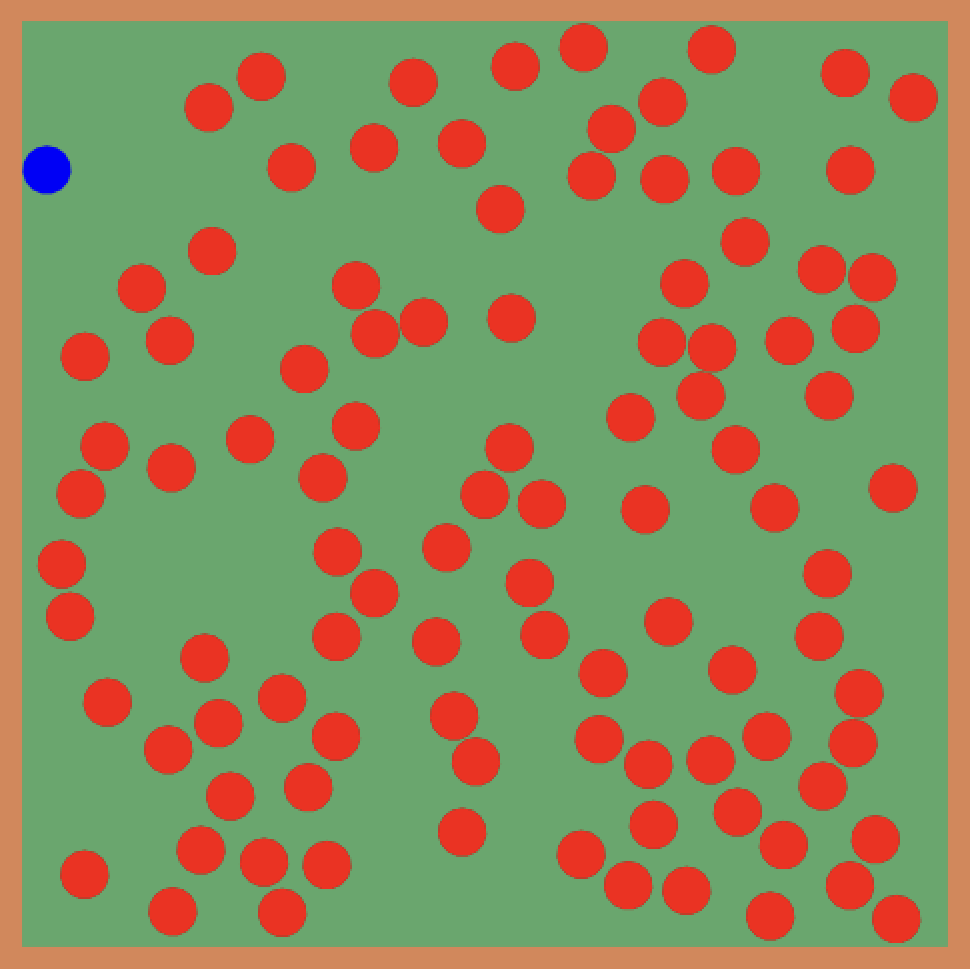
\includegraphics[width=5cm]{images/simple.png}
    \centering
    \caption{End of the simulation of a simple scenario}
    \label{simple}
 \end{figure}
 
\begin{figure} [H]
    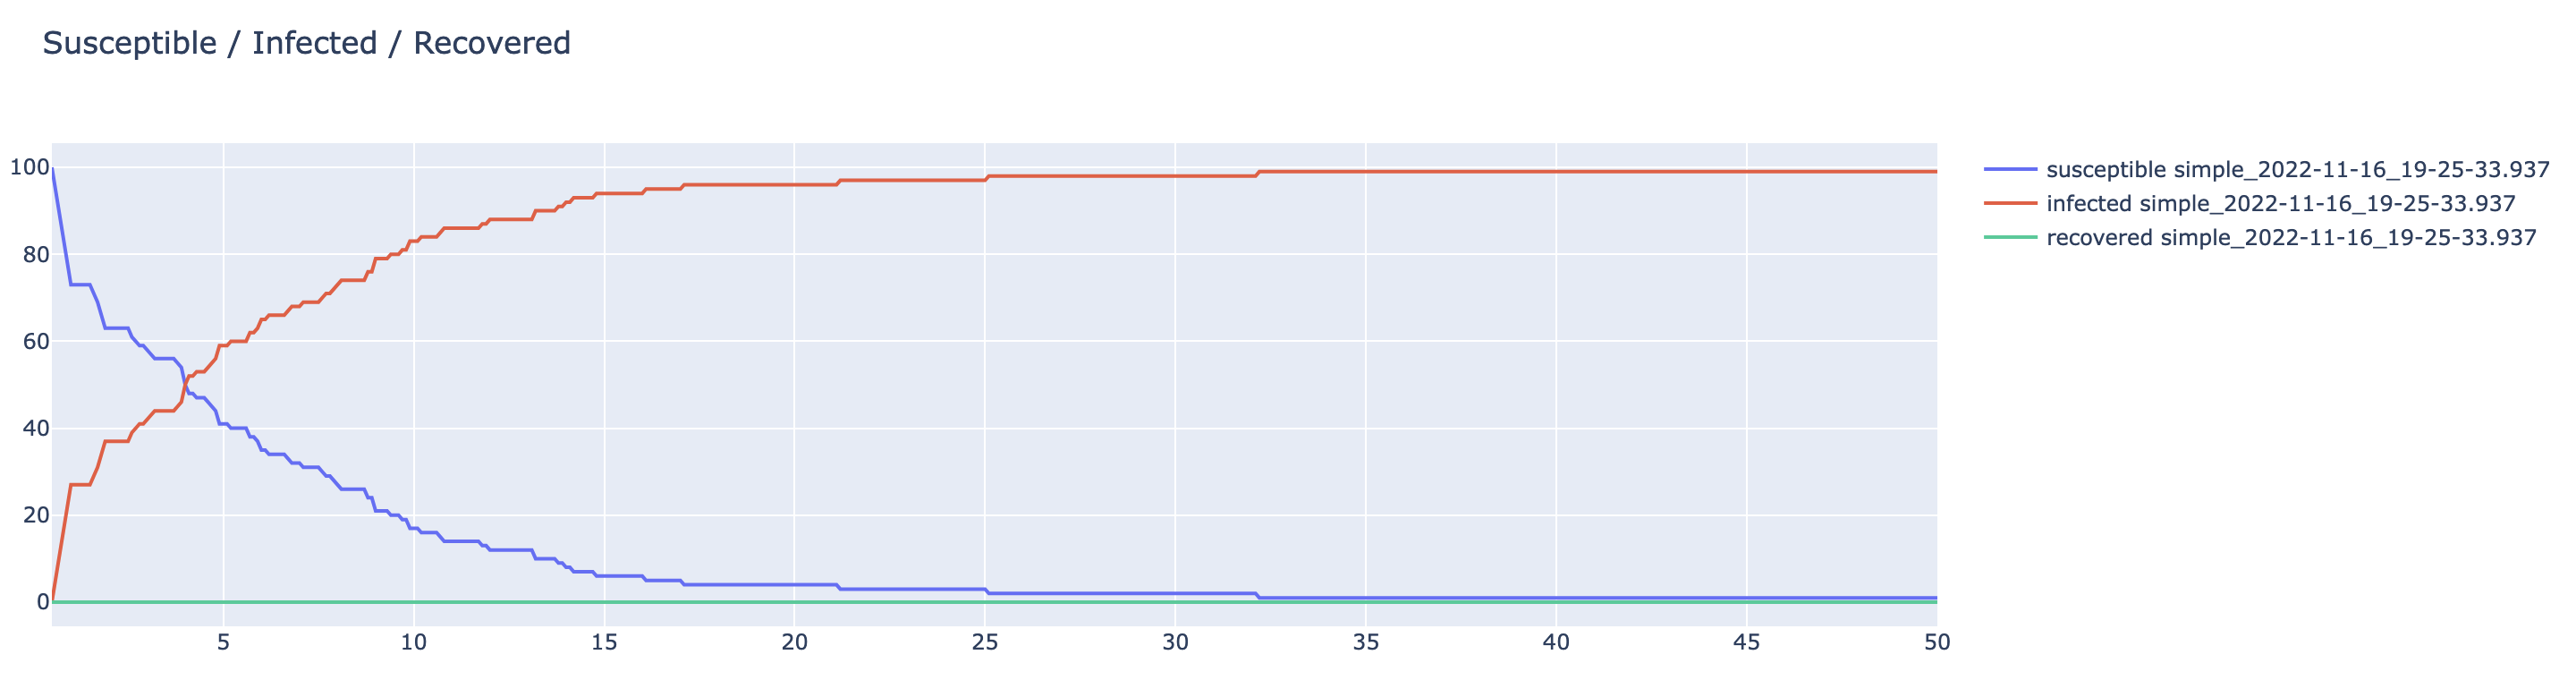
\includegraphics[width=15cm]{images/simple_evolution.png}
    \centering
    \caption{Evolution of the simulation of a simple scenario}
    \label{simple_evolution}
\end{figure}

As observed in Figure \ref{simple}, in the end of the simulation there was only one susceptible pedestrian left, who did not get infected because it was out of range of the other infected pedestrians. A representation of the evolution of the infection progress is shown in Figure \ref{simple_evolution}. This behaviour was the expected, since no recovered pedestrians are being introduced.

\bigskip

Next, the recovery rate will be set to 0.05. This means that infected pedestrians will eventually recover from the disease, thus the number of infected pedestrians will not grow up as quickly as in the previous case. At a given point, the number of infected pedestrians will only decrease until all of them get recovered.

\begin{figure} [H]
 \centering
  \subfloat[At the beginning of the simulation]{
   \label{simple_recover05a}
    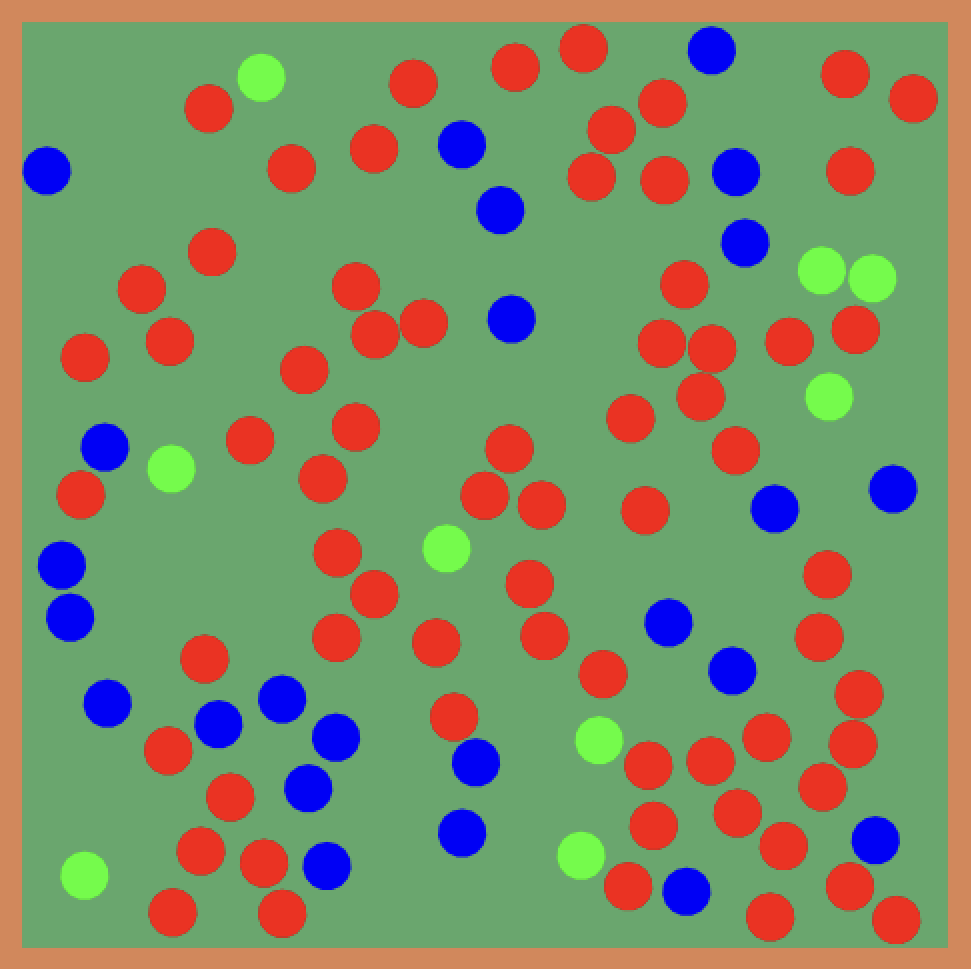
\includegraphics[width=5cm]{images/simple_recovery05a.png}}
  \subfloat[In the middle of the simulation]{
   \label{simple_recover05b}
    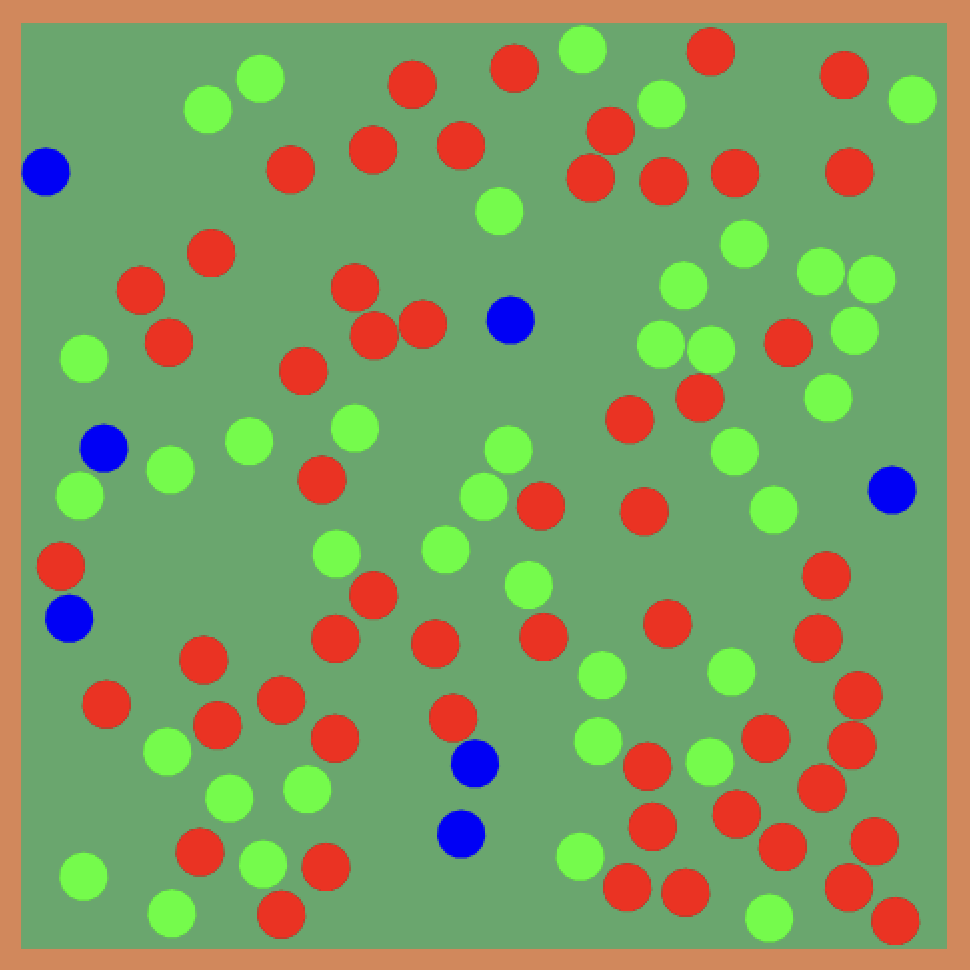
\includegraphics[width=5cm]{images/simple_recovery05b.png}}
  \subfloat[At the end of the simulation]{
   \label{simple_recover05c}
    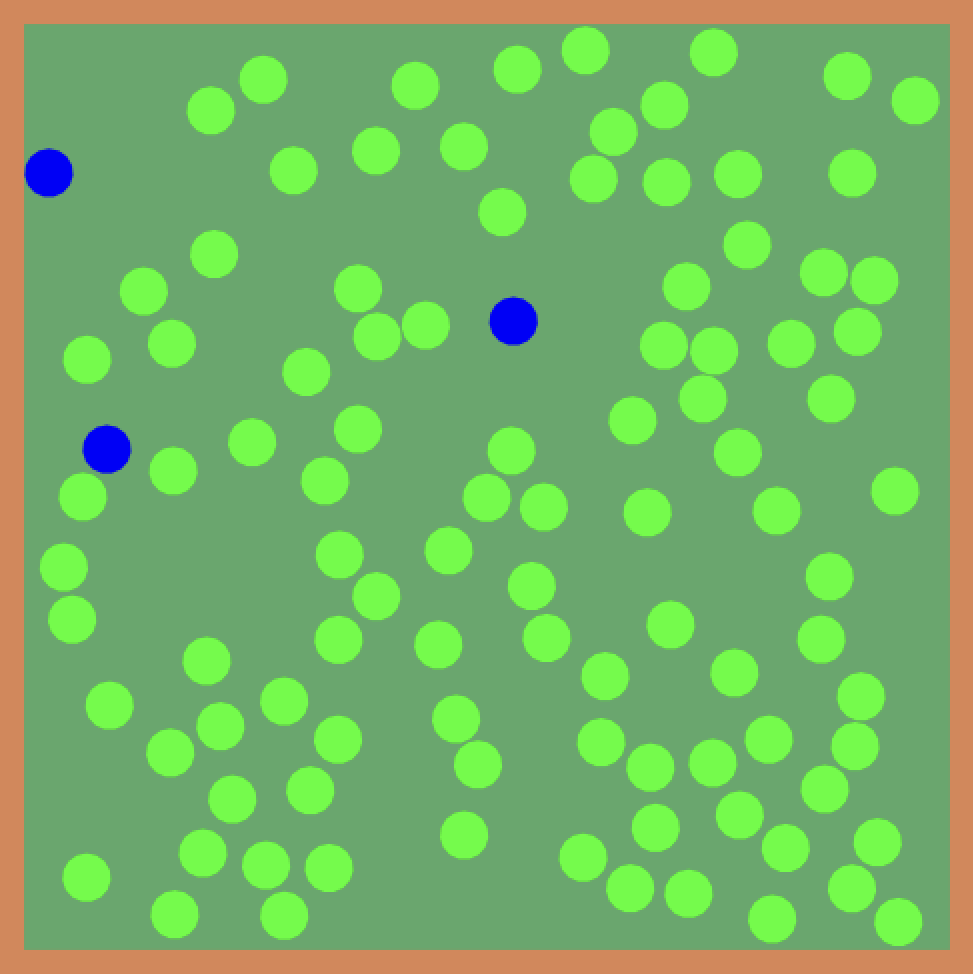
\includegraphics[width=5cm]{images/simple_recovery05c.png}}
 \caption{Different stages of the simulation of a simple scenario with recovery rate of 0.05}
 \label{simple_recover05}
\end{figure}

\begin{figure} [H]
    \includegraphics[width=15cm]{images/evolution05.png}
    \centering
    \caption{Evolution of the simulation of a simple scenario with a recovery rate of 0.05}
    \label{evolution05}
\end{figure}

As seen in Figures \ref{simple_recover05} and \ref{evolution05}, there were many more infected than recovered pedestrians at the beginning of the simulation. Later on, infected pedestrians became recovered until no infected pedestrian remained. More pedestrians remained susceptible than in the previous case, since there is the possibility of a pedestrian being able to recover before it infects all its neighbors. The implementation seems to be correct so everything is ready for the next tests.

\newpage

\noindent{\textbf{Test 1}}

This first test asks to construct a fairly large scenario with a source spawning 1000 pedestrians over a target, so that they keep still during the simulation. The aim of this test is to visualize how the susceptible, infective and recovered numbers change over time.

For this, a source with dimensions 25x25 has been placed with 1000 static pedestrians (Figure \ref{test1_scenario}. The first values set for the infection and recovery rates are going to be 0.1 and 0.05, respectively. As asked, the simulation begins with 10 infected and 990 susceptible pedestrians at the start.

\begin{figure} [H]
    \includegraphics[width=5cm]{images/test1_scenario.png}
    \centering
    \caption{Setup of the scenario for the test 1}
    \label{test1_scenario}
\end{figure}

\begin{figure} [H]
    \includegraphics[width=15cm]{images/test1_evo.png}
    \centering
    \caption{Evolution of the scenario for the test 1}
    \label{test1_evo}
\end{figure}

The result of this simulation is displayed in Figure \ref{test1_evo}. It is practically identical to the results obtained with the introductory test (Figure \ref{evolution05}), with the difference that there are ten times more pedestrians.

Again, since pedestrians can recover now, the number of infected pedestrians does not grow as quickly as before, without this new state. Around 175 pedestrians remained susceptible whether because there were not infected pedestrians in their neighborhood at any time, or because there were infected neighbors but they recovered from it before spreading it.

It should be highlighted that even though at a given point the number of infected pedestrians stopped growing, it does not mean that no more pedestrians were being infected. In fact, there were, but it kept decreasing because fewer and fewer susceptible pedestrians remained from time to time, until no more pedestrians could be infected, while already infected pedestrians kept recovering from the disease.

\newpage

\noindent{\textbf{Test 2}}

The second test asks to experiment with the infection and recovery rates in the same scenario as before, and see how the evolution of the disease changes when these parameters are changed.

Since the behaviour when the recovery rate is smaller than the infection rate has already been studied in the previous test, for the next simulations the recovery rates will be equal, higher or much higher than the infection rate, which will be kept fixed in 0.1.

\begin{figure} [H]
 \centering
  \subfloat[recoveryRate = 0.1]{
   \label{test2_01}
    \includegraphics[width=5cm]{images/test2_01.png}}
  \subfloat[recoveryRate = 0.2]{
   \label{test2_02}
    \includegraphics[width=5cm]{images/test2_02.png}}
  \subfloat[recoveryRate = 0.5]{
   \label{test2_05}
    \includegraphics[width=5cm]{images/test2_05.png}}
 \caption{End of different simulations with different recovery rates}
 \label{test2_sim}
\end{figure}

By comparing the results of the simulations using different recovery rates as shown in Figures \ref{test2_sim} and \ref{test2_evo}, it can be concluded that the higher the recovery rate is, the weaker the disease becomes, meaning that it disappears earlier. Therefore, the number of remaining susceptible pedestrians increases in relation to this parameter.

Going one step further, the relation between the recovery rate and the total number of recovered pedestrians has been studied as well. By taking a look at the plot displayed in Figure \ref{recoveryPlot}, it is remarkable how in the interval from recovery rate 0.2 to 0.3 there is a major impact on the spread of the disease. From the 0.3 ratio on, the decrease relaxes until the 0.9 ratio, where a slight increase can be noticed. This increase, however, might have been impacted by the execution of the program, but it is also a proof of the ratio not being so relevant when it is already close to 1.0.

In conclusion, it has been observed that the higher the recovery rate was, the weaker the disease became. This increase in the recovery rate resulted in a continuous decrease in the total number of recovered pedestrians, but rather than being a constant decrease, there are intervals where a major decrease can be noticed, which in this case was between the rates 0.2 and 0.3.

\begin{figure}[H]
    \includegraphics[width=15cm]{images/test2_evo01.png}
    \includegraphics[width=15cm]{images/test2_evo02.png}
    \includegraphics[width=15cm]{images/test2_evo05.png}
    \centering
    \caption{From top to bottom, evolution of the simulation with recovery rates 0.1, 0.2 and 0.5}
    \label{test2_evo}
\end{figure}

\begin{figure}[H]
\begin{tikzpicture}
 
\begin{axis}[
    xmin = 0.1, xmax = 1,
    ymin = 0, ymax = 800,
    xtick distance = 0.1,
    ytick distance = 100,
    grid = both,
    minor tick num = 1,
    major grid style = {lightgray},
    minor grid style = {lightgray!25},
    width = 15cm,
    height = 0.5\textwidth,
    xlabel = recovery rate,
    ylabel = recovered pedestrians]
 
% Plot a function
\addplot[
    smooth,
    thick,
    blue,
    mark=*
] file[skip first] {data_test2.dat};
 
\end{axis}
 
\end{tikzpicture}
\label{recoveryPlot}
\caption{Relation between the recovery rate and the number of recovered pedestrians}
\end{figure}

\newpage

\noindent{\textbf{Test 3}}

For the third test, we implemented a supermarket scenario (Figure \ref{supermarket1}) for testing the actions of customers and the result of social distancing by using different pedPotentialPersonalSpaceWidth within the process of simulation. A 50x50 scenario with 11 different kind of merchandise, 7 cashiers, a passage for customers that did not buy anything, and 1 exist as targets is manually constructed first. 

\begin{figure}[H]
    \includegraphics[width=7cm]{images/supermarket_01.png}
    \includegraphics[width=7cm]{images/supermarket_03.png}
    \centering
    \caption{The implemented supermarket topography and simulation result, showing obstacles representing shelves and walls, target areas representing different departements such as groceries and beverage products, etc., and automatically added sources of customers with different shopping list.}
    \label{supermarket1}
\end{figure}

Because we would like to simulate the real trajectories of customers travelling through different shelves buying different sort of commodities, we implemented Python code to automatically add sources of customers with different shopping lists, each of which is sampled randomly from the list of all options. A source for customers buying nothing is also added. 

Considering for simulating the varying total number of customers in the supermarket from time to time within the opening hours, the starting and ending time of generating customers of each sources is also randomly chosen within a range, which makes the total rate of adding customers varies through time, i.e., only a few sources generates customers at the beginning and the end, whereas all sources are adding customers in the middle of simulation.

In order to see the result in a more clear and efficient manner, we set the attributes of SIR model as following: the infection rate has been continued setting to 0.05 (``infectionRate": 0.05) with 10 infected pedestrians infected at the beginning (``infectionsAtStart": 10) and the maximum infection distance is set to 1.0 (``infectionMaxDistance": 1.0). The recovery rate is set to 0.005 (``recoveryRate": 0.005) as to keep the number of infected customers not decreasing too much within the supermarket. The simulation will be executed with a simulation time ratio of 1.0 (``realTimeSimTimeRatio" = 1.0) and the time step will be 0.5 (``simTimeStepLength"= 0.5). And the attribute useFreeSpaceOnly as true.

For changing the pedPotentialPersonalSpaceWidth, we tested it using value of 1.0, 3.0 and 5.0, with each of 25 sources generating 50 pedestrians throughout time in total. SIR result is shown in Figure \ref{supermarket50}:

\begin{figure}[H]
    \includegraphics[width=5.5cm]{images/supermarket_1.0_50.png}
    \includegraphics[width=5.5cm]{images/supermarket_3.0_50.png}
    \includegraphics[width=5.5cm]{images/supermarket_5.0_50.png}
    \centering
    \caption{The simulation result with each sources generatng 50 pedestrians in total, and pedPotentialPersonalSpaceWidth = 1.0, 3.0 and 5.0}
    \label{supermarket50}
\end{figure}

From which we can see that such social distance does help a little to reduce the number of infections. The final ratio of customers being infected has reduced from around $80\%$ to $50\%$ with the social distance increased five-times. Yet it is still too crowded for further reduction in infection cases within the supermarket, and increasing social distance also caused more time in serving all the customers.

Considering restricting the total amount of customers entering into the supermarket from the beginning. We reduce the number of pedestrians generated by each sources from 50 to 25 and 10. The result is shown in Figure \ref{supermarket25} and Figure \ref{supermarket10}:

\begin{figure}[H]
    \includegraphics[width=5.5cm]{images/supermarket_1.0_25.png}
    \includegraphics[width=5.5cm]{images/supermarket_3.0_25.png}
    \includegraphics[width=5.5cm]{images/supermarket_5.0_25.png}
    \centering
    \caption{The simulation result with each sources generatng 25 pedestrians in total, and pedPotentialPersonalSpaceWidth = 1.0, 3.0 and 5.0}
    \label{supermarket25}
\end{figure}

\begin{figure}[H]
    \includegraphics[width=5.5cm]{images/supermarket_1.0_10.png}
    \includegraphics[width=5.5cm]{images/supermarket_3.0_10.png}
    \includegraphics[width=5.5cm]{images/supermarket_5.0_10.png}
    \centering
    \caption{The simulation result with each sources generatng 10 pedestrians in total, and pedPotentialPersonalSpaceWidth = 1.0, 3.0 and 5.0}
    \label{supermarket10}
\end{figure}

As it is shown in the graphs, restricting total customer flow is far more effective than simply forcing a larger social distance. With half traffic flow, the ratio of infected cases for the social distance 1.0 has rapidly dropped around $20\%$ instead of the original $80\%$ (especially considering that half of them is the infected cases introduced at the beginning, which means the actual ratio is around $10\%$); and a one-fifth customer flow has even managed to keep the number of infected staying the same as the number of pedestrians infected set at the beginning (10), with only less than 5 customers get themselves infected within our supermarket. And conducting social distance policy even worsened the case, since customers cannot get themselves into shelves and cashiers they want to reach as rapidly as before, which caused everyone spending much more time in the supermarket and increased their probabilities of getting infected.

Therefore, conducting social distance policy can reduce the infection cases, whereas controlling the amount of customers entering into our supermarket is far more effective. This can be achieved in the real world by extending opening hours, or providing discounts during less populous hours to encourage customers to visit when the store is not busy.

\bigskip

\noindent{\textbf{Bonus Test 1}}

Here, we test the case when half of the cashiers were closed. This should increase the total amount of time customers spend within the supermarket, especially in the case of high customer traffic. And the situation could even get worse, because the waiting area for cashiers has the most density of customers, further increase the probability of getting infected.


\begin{figure}[H]
    \includegraphics[width=8cm]{images/bonus_1.png}
    \centering
    \caption{Closing half of the cashiers makes too many customers gathering around the cashier area}
    \label{bonus1-1}
\end{figure}


\begin{figure}[H]
    \includegraphics[width=5.5cm]{images/bonus1_1.0.png}
    \includegraphics[width=5.5cm]{images/bonus1_3.0.png}
    \includegraphics[width=5.5cm]{images/bonus1_5.0.png}
    \centering
    \caption{The simulation result with removing half cashiers, each sources generating 100 pedestrians in total, and pedPotentialPersonalSpaceWidth = 1.0, 3.0 and 5.0}
    \label{bonus1-2}
\end{figure}

As Figure \ref{bonus1-2} shows, closing half cashiers has significantly increased cases of infections, caused an increase in total time customers spent in the supermarket, and also makes social distance become way less effective than before.


\bigskip

\noindent{\textbf{Bonus Test 2}}

Here, we test the case when 1/3 of the shelves were removed. This should also increase the total amount of time customers spend within the supermarket, especially in the case of high customer traffic. The situation should similar to removing cashiers, as it increase the time for customers to find the commodities they wish to get.


\begin{figure}[H]
    \includegraphics[width=8cm]{images/bonus2.png}
    \centering
    \caption{The scenario of removing 1/3 of the shelves}
    \label{bonus2}
\end{figure}


\begin{figure}[H]
    \includegraphics[width=5.5cm]{images/bonus2_1.0.png}
    \includegraphics[width=5.5cm]{images/bonus2_3.0.png}
    \includegraphics[width=5.5cm]{images/bonus2_5.0.png}
    \centering
    \caption{The simulation result with closing 1/3 of shelves, each sources generating 100 pedestrians in total, and pedPotentialPersonalSpaceWidth = 1.0, 3.0 and 5.0}
    \label{bonus2-2}
\end{figure}

As Figure \ref{bonus2-2} shows, removing shelves also increased cases of infections, caused an increase in total time customers spent in the supermarket, and makes social distance become way less effective than before as well. The case is even worse than reducing cashiers, as during the process of customers fetching products they are actually passing by and interacting with more people than waiting in the cashier zone.


\bigskip

\noindent{\textbf{Bonus Test 3}}

Here, we would like to test our supermarket's full capacity of serving customers. The amount of customers generated by each sources is set to 200, and number of sources also increased from 25 to 49. We are using the topology scenario same as the one in test 3.


\begin{figure}[H]
    \includegraphics[width=8cm]{images/bonus3.png}
    \centering
    \caption{The extreme scenario with four times in total amount of customers}
    \label{bonus3}
\end{figure}

\begin{figure}[H]
    \includegraphics[width=12cm]{images/bonus3-2.png}
    \centering
    \caption{A tremendous amount of infections has happened}
    \label{bonus3-2}
\end{figure}

As Figure \ref{bonus3} and \ref{bonus3-2} shows, We can observe that a huge crowd of pedestrians gathered in the middle of the supermarket. With this number of crowds, as one can expect a tremendous amount of infections has happened.



\end{task}

\bibliographystyle{plain}
\bibliography{Literature}

\end{document}

